% !TeX root = ../main.tex

%\chapter{\texorpdfstring{Measurement of ZZ Production with $ll\nu\nu$ Final State}{Measurement of ZZ Production with llnunu Final State}}
%\label{chap:llvv_analysis}


\section{Overview}
\label{sec:ZZ_intro}

Conducting diboson production studies at the Large Hadron Collider is essential for the contemporary particle physics agenda, as it imposes incredibly rigorous stress tests on the Standard Model. This research specifically grants direct observational access to the underlying electroweak gauge geometry—most notably, the non-Abelian self-coupling mechanisms governing gauge bosons, as detailed earlier in Section~\ref{boson-interactions}.
%
Within the diverse family of diboson events, generating pairs of $Z$ bosons ($ZZ$) commands distinct attention. At the foundational tree level, the SM completely prohibits any interactions driven exclusively by neutral gauge bosons. Consequently, this specific decay avenue becomes highly responsive to anomalous theoretical inputs stemming from physics beyond the Standard Model (BSM), where such forbidden interactions might realistically emerge.
%
For this reason, achieving high-precision evaluations of the $ZZ$ overall production cross section establishes a robust testing ground for SM validity at maximum collision energies. Simultaneously, it delivers exceptional sensitivity for detecting new-physics footprints, including the presence of anomalous triple-gauge couplings (aTGCs).

Using extensive datasets harvested at collision energies of $\sqrt{s} = 7$, $8$, $13$, and $13.6$~TeV, thorough evaluations of the $ZZ$ production cross sections have been published by both the CMS Collaboration~\cite{CMS-SMP-12-007, CMS-SMP-13-005, CMS-SMP-16-001, CMS-SMP-19-001} and the ATLAS Collaboration~\cite{ATLAS:2013zz,ATLAS:2017zz,ATLAS:2018zz,STDM-2017-03,STDM-2022-17,ATLAS:2024zz_13p6}. 
These comprehensive investigations have uniformly verified an outstanding alignment with expected Standard Model behavior, confidently confirming perturbative QCD computations up to next-to-next-to-leading order (NNLO), alongside electroweak corrections calculated at next-to-leading order (NLO). Additionally, because these high-resolution measurements revealed zero meaningful departures from SM baselines, both experimental collaborations successfully enforced progressively tighter boundaries on anomalous quartic gauge couplings (aQGCs) as well as neutral aTGCs. Analytically, these efforts primarily rely on two distinct yet complementary topological signatures generated by decaying $Z$ boson pairs: the semi-invisible tracking channel comprising two neutrinos coupled with two charged leptons ($\ell\ell\nu\nu$), and the purely leptonic channel featuring four explicitly identified charged leptons ($4\ell$).

%\subsection{Motivation for the $\ell\ell\nu\nu$ Channel}
Although the highly prized $ZZ \to 4\ell$ ``golden channel'' guarantees a flawlessly reconstructed event topology accompanied by pristine signal purity, its utility is severely hampered by an inherently narrow branching ratio. Conversely, the statistical probability of a $Z$ boson decaying into paired neutrinos ($\mathcal{B}(Z \to \nu\bar{\nu}) \approx 20\%$) outpaces the charged-lepton decay route ($\mathcal{B}(Z \to \ell^+\ell^-) \approx 3.3\%$ per specific lepton flavor) by roughly a factor of six.
%
Consequently, analyses leveraging the $ZZ \to \ell^+\ell^-\nu\bar\nu$ pathway capitalize on a dramatically amplified event yield, which directly translates into vastly superior statistical precision across the board.

Securing this statistical leverage becomes exceptionally critical when probing the extreme high transverse momentum ($p_{\mathrm{T}}$) sectors. Any theorized deviations from standard SM behavior—whether they manifest through novel heavy resonances or via effective field theory (EFT) mechanics—are overwhelmingly projected to amplify at these upper energy limits. Given this theoretical landscape, the $\ell\ell\nu\nu$ decay profile secures a definitive advantage over the $4\ell$ alternative in terms of isolating and identifying potential aTGCs.

Furthermore, mastering the exact dynamics of the $ZZ \to \ell^+\ell^-\nu\bar\nu$ event stream is absolutely mandatory for background mitigation. It acts as the dominant irreducible background signature for two major research fronts: the pursuit of high-mass Higgs bosons decaying to $ZZ$ within identical final states, and the hunt for dark matter utilizing mono-$Z$ event topologies.

The core objective of this chapter is to deliver a comprehensive breakdown of the latest $ZZ$ production measurement executed using proton–proton impacts at $\sqrt{s} = 13$~TeV. This analysis leverages the complete Run~2 data portfolio captured by the ATLAS instrument, which totals an integrated luminosity of $140~\text{fb}^{-1}$~\cite{ATLAS:2025_ZZ_llvv}. This updated result drastically surpasses the prior experimental benchmark, which relied on a mere 36~fb$^{-1}$ dataset and reported a precision margin of 7.0\%~\cite{ATLAS:2019zz_llvv}. Specifically, the study homes in on the $ZZ \rightarrow \ell^+\ell^- \nu \bar{\nu}$ decay sequence, wherein one $Z$ boson shatters into neutrinos while its partner yields charged leptons ($\ell = e, \mu$). This interaction leaves behind a highly recognizable trace: an energetic dilepton pairing derived from the visible $Z$ boson, coupled with a massive spike in missing transverse momentum ($\ell^+\ell^- + E_\text{T}^\text{miss}$). Additionally, the scope of this investigation includes generating differential cross-section calculations across a broad spectrum of kinematic variables. To hunt for new physics, the study imposes strict limits on anomalous gauge boson self-couplings. These boundaries are calculated systematically via the Effective Field Theory paradigm~\cite{Degrande:2013} as well as the standard effective vertex function framework~\cite{Hagiwara:1987}.

\section{Analysis Strategy and Outline}

The extraction of this measurement is strictly confined to a fiducial phase space that closely mimics the actual physical acceptance limits of the detector. During event filtering, the pipeline isolates collisions that feature a clear dilepton pairing mathematically compatible with the invariant mass of a $Z$ boson, simultaneously paired with a substantial surge in missing transverse momentum ($E_{\mathrm{T}}^{\text{miss}}$) injected by the escaping neutrinos.

However, several background interactions can deceptively replicate this signal trace, most notably $Z$+jets collisions, alternative diboson events ($WZ$, $WW$), and standard top-quark generation. To accurately quantify and subtract these contaminants, the analysis relies heavily on specialized control regions that are deliberately engineered to be rich in those exact background processes.

Ultimately, the final physics parameters are extracted by executing a simultaneous mathematical fit applied directly to the empirical data spanning both the control regions (CRs) and the core signal region (SR). These fitted results are then rigorously cross-examined against theoretical baselines derived from MC models.

The structural flow of this analytical presentation is organized as follows:
\begin{itemize}
    \item A comprehensive review of the MC simulation grids and raw data sets deployed to construct both background and signal models is provided in Section~\ref{sec:llvv_samples}.
    \item The methodologies defining the Signal Regions (SR), alongside the exact criteria used for reconstructing isolated physics objects, are explained in Section~\ref{sec:llvv_selection}.
    \item The strategy for calculating major background interference—focusing heavily on non-resonant contamination (like $WW$ and top quarks) as well as the primary $WZ$ background—via data-driven control regions is laid out in Section~\ref{sec:llvv_background}.
    \item A detailed breakdown of all theoretical and experimental sources contributing to systematic uncertainty is cataloged in Section~\ref{sec:llvv_systematics}.
    \item The specialized unfolding mechanics utilized to map raw detector-level event distributions back to the true particle level are outlined in Section~\ref{sec:llvv_unfolding}.
    %\item Section~\ref{sec:llvv_dnn} describes the optimization strategies, including the use of Deep Neural Networks (DNN), to enhance the separation between signal and background.
    \item The final derived constraints limiting aTGCs, alongside the calculated differential and integrated cross-sections mapping inclusive $ZZ$ generation, are disclosed in Section~\ref{subsec:diff-xs}.
    \item Lastly, Section~\ref{subsec:aqgc_limits} pushes the analytical boundaries to examine the electroweak generation of $ZZ$ paired with two distinct jets ($ZZjj$), specifically hunting for anomalous Quartic Gauge Couplings (aQGCs) within Vector Boson Scattering (VBS) event topologies.
\end{itemize}
%%%%%%%%%%%%%%%%%%%%%%%%%%%
\section{Monte Carlo and Data Samples}
\label{sec:llvv_samples}

The specific simulated samples and empirical datasets utilized throughout this analysis are outlined in this section. Captured by the ATLAS detector between 2015 and 2018, the Run~2 $pp$ collision dataset operates at a center-of-mass energy of $\sqrt{s} = 13~\text{TeV}$.

By merging detailed detector response models with theoretical predictions, Monte Carlo (MC) simulations serve a critical function in profiling the topological and kinematic traits of the signal, while also quantifying the expected yields from all major SM backgrounds.

Maintaining consistency in event selection rules, calibration routines, and physics object reconstruction across both simulated samples and actual data remains a cornerstone of this study. Such a unified methodology guarantees an impartial, direct alignment between theoretical models and observed events, ultimately securing the reliability of the extracted physics outcomes.

The subsequent subsections initially present an exhaustive summary of the MC models generated for various background and signal processes. Following this, the discussion breaks down the exact data samples, the applied data quality restrictions, and the specific trigger logic leveraged to isolate analysis events. Exhaustive inventories containing dataset identifiers (DSIDs), trigger chains, generator parameters, and Good Run Lists are cataloged in Appendix~\ref{subsec:samples_zz}.

\subsection{The ATLAS Simulation Framework}
Generating simulated events within the ATLAS collaboration adheres to a highly standardized sequential pipeline, which reliably mirrors proton--proton interactions and the subsequent hardware responses. This simulation workflow is anchored by three primary phases:

\begin{enumerate}
    \item \textbf{Event Generation:} The fundamental hard-scatter collision is replicated utilizing an array of event generators. These specialized programs calculate the matrix element (ME) governing a given physical interaction, typically achieving leading order (LO) or next-to-leading order (NLO) accuracy within perturbative QCD. Subsequently, this ME evaluation is linked to a parton shower (PS) framework—such as the integrated module within \textsc{Sherpa}~\cite{Bothmann_2019} or the standalone \textsc{Pythia}~8~\cite{Sjostrand:2014zea} algorithm. This PS stage simulates particle decays, hadronization, multiple parton interactions, as well as final- and initial-state radiation. For every individual sample, the designated PDF (Parton Distribution Function) set, perturbative precision, and specific generator are carefully selected to yield the highest-fidelity process modeling.

    \item \textbf{Detector Simulation:} Utilizing the \textsc{Geant4} software suite~\cite{GEANT4:2002zbu}, the stable particles produced during the initial generation phase are tracked as they traverse a meticulous digital replica of the ATLAS detector's material makeup and spatial geometry. This crucial step models the exact physical interactions between the traversing particles and the detector's passive and active components, generating simulated ``hits'' and energy deposits across the sub-systems.

    \item \textbf{Digitisation and Reconstruction:} These artificial detector hits are subsequently translated into digitized electronic pulses, closely mimicking authentic hardware readouts. To accurately reflect the LHC's intense high-luminosity conditions, numerous inelastic $pp$ collisions—commonly referred to as pile-up—are superimposed onto every simulated hard-scatter event. To model these pile-up interactions, \textsc{Pythia}~8 is employed alongside the \textsc{NNPDF2.3LO} PDF set~\cite{Ball:2012cx} and the A3 tune~\cite{ATL-PHYS-PUB-2016-017}. Furthermore, the simulated pile-up multiplicity distribution is explicitly reweighted to mirror the exact profile observed in the empirical data. As a final step, the simulated digital output is fed through the exact same reconstruction software used for genuine collision data, ultimately assembling high-level physics objects like jets, missing transverse momentum ($E_{\text{T}}^{\text{miss}}$), electrons, and muons.
\end{enumerate}

To reconcile minor discrepancies in identification, reconstruction, and trigger efficiencies between the MC simulations and empirical data, specific scale factors (or correction weights) are systematically applied to all simulated datasets.


\subsection{Monte Carlo Samples}

Deriving accurate background estimations and signal efficiencies necessitates a broad portfolio of MC event samples. These datasets are explicitly generated to align with the operating conditions of the 2015--2018 data-taking campaigns, and they undergo the exact same calibration algorithms and reconstruction software pipelines as the physical collision data. This rigid symmetry ensures that all physics objects are handled consistently, authorizing a seamless comparison between theoretical expectations and experimental observations. The ensuing segments outline the specialized generators tasked with simulating both background and signal activities. 


\subsubsection{Signal Samples}
This study is fundamentally geared toward measuring the inclusive SM $\text{ZZ}$ production cross-section within the $\ell^+\ell^-\nu\bar{\nu}$ decay topology, simultaneously probing for BSM phenomena via anomalous gauge boson couplings.

\paragraph{Standard Model $\text{ZZ}$ Production}
The dominant signal topology involves the creation of paired $\text{Z}$ bosons that subsequently decay into the $\ell^+\ell^-\nu\bar{\nu}$ final state. This encompasses loop-mediated gluon-gluon fusion as well as quark-antiquark annihilation pathways, both of which are modeled utilizing \textsc{Sherpa}~2.2.2. Conversely, the electroweak generation of $\text{ZZ}$ accompanied by two jets is simulated independently using \textsc{MadGraph5}~\cite{Alwall:2014hca}. 
Table~\ref{tab:sherpa-xs} displays the resulting MC-derived cross-sections for both the $\text{ZZ}jj$ and $\text{ZZ}$ fiducial phase spaces. An exhaustive inventory of these generated samples—featuring their associated k-factors and DSIDs—can be referenced in Appendix~\ref{subsec:samples_zz} (specifically Table~\ref{tab:ZZ_signal_samples}).

\begin{table}[htbp]
\centering
\small
\renewcommand{\arraystretch}{1.4}
\begin{tabular}{l c}
\hline
\textbf{Cross-section}  & \textbf{Calculated value [fb] } \\
\hline
$\sigma^{\text{fid}}_{\text{ZZ} \to \ell\ell\nu\nu}$ & $20.08 \pm 1.0_{\text{scale}} \pm 0.30_{\text{PDF}} \pm 0.24_{\alpha_S}$ \\
$\sigma^{\text{fid}}_{\text{ZZ}jj \to \ell\ell\nu\nu jj}$ & $0.94 \pm 0.19_{\text{scale}} \pm 0.01_{\text{PDF}} \pm 0.02_{\alpha_S}$ \\
\hline
\end{tabular}
\caption{Fiducial cross-sections for $\text{ZZ} \to 2\ell 2\nu$ and $\text{ZZ}jj \to 2\ell 2\nu jj$ productions at $\sqrt{s} = 13~\text{TeV}$. The $\text{ZZ}$ and $\text{ZZ}jj$ cross-sections are obtained with the QCD production simulated using \textsc{Sherpa} and the electroweak production simulated using \textsc{MadGraph5} (NLO EW). Theoretical uncertainties from QCD scale variation, PDFs, and $\alpha_S$ are quoted.}
\label{tab:sherpa-xs}
\end{table}

\paragraph{Samples with Anomalous Gauge Couplings}
The hunt for new physics relies on evaluating anomalous quartic gauge couplings (aQGC) alongside anomalous neutral triple gauge couplings (nTGC) through the lens of an Effective Field Theory (EFT) framework. To accurately replicate the kinematic distortions introduced by these BSM operators, a specialized batch of MC samples was synthesized. Comprehensive DSID registries cataloging the aQGC and nTGC search models are provided in Tables~\ref{tab:ZZEFTsamples} and~\ref{tab:ZZaQGCsamples} within Appendix~\ref{subsec:samples_zz}.


\subsubsection{Background Samples}
Contaminating backgrounds infiltrating the $\ell^+\ell^- + E_{\text{T}}^{\text{miss}}$ target state are generally classified into two camps: reducible backgrounds triggered by severe detector mismeasurements or misidentified objects, and irreducible backgrounds characterized by genuine $E_{\text{T}}^{\text{miss}}$ paired with prompt leptons. Exhaustive data tables cataloging these background samples are available in Appendix~\ref{subsec:samples_zz}.

\paragraph{Diboson and Triboson Backgrounds}
The most prominent irreducible background interference stems from the generation of $\text{WW}$, $\text{WZ}$, and fully leptonic $\text{ZZ} \to \ell^+\ell^-\ell^+\ell^-$ events. Minor contamination originating from triboson processes (such as $\text{ZZZ}$, $\text{WZZ}$, $\text{WWZ}$, and $\text{WWW}$) is similarly accounted for. These specific interactions are primarily simulated via \textsc{Powheg}+\textsc{Pythia}~8 and \textsc{Sherpa} (refer to Tables~\ref{tab:ZZbkg_samples},~\ref{tab:WZandWWsamples}, and~\ref{tab:VVVsamples}).

\paragraph{Top Quark Backgrounds}
Another dominant background source arises from single-top and top-antitop ($t\bar{t}$) generation, specifically leaking through their dileptonic decay branches. Top quark production occurring in association with a vector boson ($t\bar{t}\text{V}$) provides an additional contribution. To model these events, \textsc{MadGraph5\_aMC@NLO} and \textsc{Powheg}+\textsc{Pythia}~8 are deployed (see Tables~\ref{tab:Topsamples} and~\ref{tab:ttVsamples}).

\paragraph{$\text{Z}/\gamma^*$+jets Background}
Acting as the primary reducible background, this contamination originates from Drell-Yan processes plagued by artificially inflated, mismeasured $E_{\text{T}}^{\text{miss}}$. The \textsc{Sherpa}~2.2.1 generator, equipped with NLO-accurate matrix elements, is tasked with modeling this behavior. These specific samples are partitioned by lepton flavor and generated across discrete slices of the partonic transverse momentum sum (documented in Tables~\ref{tab:ZjetsSamplesSherpa1},~\ref{tab:ZjetsSamplesSherpa2}, and~\ref{tab:ZjetsSamplesSherpa3}).

\paragraph{Higgs Boson Backgrounds}
Interactions resulting in the creation of a Higgs boson can occasionally mimic the targeted final state. These relatively minor background contributions are replicated utilizing \textsc{Powheg}+\textsc{Pythia}~8 (detailed in Table~\ref{tab:Higgssamples}).


\subsection{Data Samples}

The empirical dataset is analyzed utilizing the conventional ATLAS Release 21 software environment. Stringent filters are applied so that only events captured while all detector sub-systems were fully operational and beam conditions remained perfectly stable are admitted. To enforce this, the official Run~2 Standard Good Run Lists (GRL), curated by the ATLAS Data Quality team for the 2015--2018 operational windows, are utilized, securing an integrated luminosity of $140~\text{fb}^{-1}$. The precise GRL file directories referenced for each distinct data-taking epoch are recorded in Table~\ref{tab:grls_app} of Appendix~\ref{subsec:samples_zz}.

To guarantee a highly resilient and encompassing acceptance rate for events featuring at least one energetic lepton, the selection algorithm enforces a logical disjunction (OR) spanning multiple trigger paths. By fusing di-lepton-seeded triggers with single-lepton variants, this comprehensive trigger strategy maximizes event recovery across an expansive kinematic phase space. 

Implementing this dual-trigger approach is essential to salvage signal events where the transverse momentum of an individual lepton might dip below the activation threshold required by the dominant high-$p_{\text{T}}$ single-lepton triggers. Consequently, events are harvested using a fused array of un-prescaled single-muon and single-electron triggers. Depending on the applied isolation and identification strictness (e.g., tight or medium likelihood criteria), lepton flavor, and the specific data-taking year, the lowest transverse momentum floors for these triggers fluctuate between 20~GeV and 26~GeV. For leptons exhibiting substantially higher transverse momenta (for instance, exceeding 140~GeV or 50~GeV), supplementary triggers featuring relaxed identification parameters are activated to further patch efficiency gaps. A complete and exhaustive breakdown of the specific software trigger chains deployed throughout this study is laid out in Table~\ref{tab:lepton_triggers_app} of Appendix~\ref{subsec:samples_zz}.
\section{Object and Event Selection} 
\label{sec:llvv_selection}

To successfully separate the scarce signal events from the overwhelming particle multiplicity generated during proton--proton collisions, researchers must deploy a highly rigorous extraction protocol targeting specific final-state objects. This workflow initiates with the raw electronic impulses captured by the ATLAS detector, translating them into reconstructed physical entities—namely jets, muons, and electrons. An extensive breakdown of this ATLAS object reconstruction methodology is provided in Chapter~\ref{chap:recon}. Once reconstructed, these objects are filtered through an uncompromising gauntlet of selection criteria. This ensures the retention of high-fidelity candidates and optimal signal efficiency while aggressively pruning misidentified tracks and background noise, ultimately elevating the sample's purity.

The entirety of the event filtering methodology is detailed in this segment, executing sequentially across two distinct phases. Initially, rigid thresholds are established to isolate individual physics objects, securing a meticulously calibrated, clean dataset for downstream analysis. Subsequently, entire collision events are evaluated based on this pool of reconstructed objects, specifically aiming to isolate the target signal topology and establish the ultimate signal regions.

These filtering protocols are enforced in strict accordance with the ATLAS Collaboration's formal guidelines. Comprehensive documentation listing the specific simulation campaign tags, derivation formats, and software releases harnessed for this study can be found in Appendix~\ref{subsec:samples_zz}.

% ======================================================================
\subsection{Object Selection}
\label{sec:llvv_object_selection}

Accurately isolating the targeted final state heavily depends on meticulously reconstructing and filtering its baseline physics objects out of a chaotic collision environment. This subsection outlines the exact parameters governing the acceptance of jets, electrons, and muons, which collectively construct the analytical foundation. As a concluding precaution, a spatial ambiguity resolution protocol is applied to guarantee that every selected signature is uniquely classified. All extraction parameters align flawlessly with the official configurations dictated by the ATLAS Combined Performance groups. The precise algorithm designations and software working points are cataloged in Appendix~\ref{subsec:samples_zz}.

\subsubsection{Muons}
This study leverages muons formally classified as \textit{combined muons}. These candidates are synthesized by successfully correlating a trajectory within the inner detector (ID) against an overlapping track inside the muon spectrometer. Utilizing this combined fitting technique produces exceptionally pure muon candidates equipped with highly accurate momentum readings.
%
Any signal muon incorporated into this analysis is mandated to pass a severe battery of tests confirming it is both well-isolated and strictly prompt (emanating directly from the primary collision).
\begin{itemize}
    \item \textbf{Kinematics:} Candidate muons are required to fall within the physical detector acceptance of $|\eta| < 2.5$ while registering a transverse momentum of $p_{\text{T}} > 20~\text{GeV}$.
    \item \textbf{Identification:} The algorithm enforces a ``medium-level'' identification standard. By demanding strict compatibility between the muon spectrometer and ID track fits, this criterion drastically curtails background contamination caused by misidentified hadronic tracks.
    \item \textbf{Prompt:} To systematically eliminate cosmic-ray interference and non-prompt muons generated by heavy-flavour decay chains, tight restrictions are applied to the track's impact parameters relative to the primary vertex. The transverse impact parameter significance must obey $|d_0/\sigma(d_0)| < 3$, alongside a longitudinal impact parameter boundary of $|z_0 \cdot \sin(\theta)| < 0.5~\text{mm}$.
    \item \textbf{Isolation:} To verify that the candidate is completely detached from any jet activity, an isolation boundary is enforced. This metric evaluates the combined calorimeter and track energy deposits inside a surrounding cone of $\Delta R = \sqrt{(\Delta\eta)^2+(\Delta\phi)^2} = 0.2$. The analysis adopts a ``loose'' particle-flow isolation working point, effectively yielding a $\sim$99\% retention efficiency for high-$p_{\text{T}}$ muons.
\end{itemize}
To rectify minor deviations between simulated models and empirical data, dedicated smearing and scale correction weights are applied directly to the simulated muon momenta, coupled with efficiency scale factors to balance MC yields. Furthermore, a highly relaxed baseline threshold—demanding only $p_{\text{T}} > 7~\text{GeV}$ alongside minimized identification rules—is utilized strictly to flag extra muons for event veto logic.

\subsubsection{Electrons}
Electron candidates are formed by linking an ID track to an overlapping energy deposition cluster inside the electromagnetic calorimeter. To qualify as a signal electron, the object must satisfy the following constraints:
\begin{itemize}
    \item \textbf{Kinematics:} Electron candidates are confined to the fiducial pseudorapidity volume of $|\eta| < 2.47$ and must exhibit $p_{\text{T}} > 20~\text{GeV}$.
    \item \textbf{Identification:} A multivariate likelihood discriminant—synthesizing track-cluster alignment, spatial shower topographies, and overall track quality—is leveraged for positive identification. The ``medium-level'' working point is deliberately selected, balancing optimal signal retention against robust rejection of faked electron signatures stemming from jets.
    \item \textbf{Prompt:} Mirroring the muon logic, impact parameter thresholds guarantee that electrons are born directly at the primary vertex. These limits are defined as $|z_0 \cdot \sin(\theta)| < 0.5~\text{mm}$ and $|d_0/\sigma(d_0)| < 5$.
    \item \textbf{Isolation:} To effectively discard non-prompt electrons and certify spatial separation, candidates must clear a ``loose'' particle-flow isolation boundary measured within a $\Delta R = 0.2$ cone.
    \item \textbf{Quality Veto:} During the 2015--2016 operational window, any event harboring an electron localized within the notoriously problematic transition crack of the electromagnetic calorimeter ($1.37 < |\eta| < 1.52$) is immediately vetoed. This precaution prevents severe miscalculations of the event's missing transverse momentum.
\end{itemize}
To ensure the simulation faithfully mirrors actual hardware performance, appropriate efficiency scale factors alongside energy resolution and scale corrections are injected into the MC data. Similar to the muon protocol, a relaxed baseline electron definition ($p_{\text{T}} > 7~\text{GeV}$ with highly loose likelihood constraints) is maintained explicitly for event vetoing operations.

\subsubsection{Jets}
Capturing the event's hadronic dynamics relies on jets, which are absolutely essential for constructing the VBS-like signal geometry.
\begin{itemize}
    \item \textbf{Reconstruction:} Utilizing a radius parameter of $R=0.4$, jets are clustered from baseline particle-flow objects via the anti-$k_t$ algorithm.
    \item \textbf{Kinematics and Cleaning:} Accepted jets must fall within $|\eta| < 4.5$ and register $p_{\text{T}} > 30~\text{GeV}$. Furthermore, they are subjected to mandatory cleaning heuristics to filter out spurious spikes caused by non-collision artifacts or internal detector noise.
    \item \textbf{Pileup Suppression:} To aggressively combat the noise introduced by concurrent proton--proton interactions (pileup), any jet measuring $p_{\text{T}} < 60~\text{GeV}$ situated within the tracking volume ($|\eta| < 2.4$) must successfully clear the Jet Vertex Tagger (JVT) discriminant threshold.
    \item \textbf{$b$-Jet Veto:} The production of top-quark pairs injects massive background interference. To suppress this, any event containing a tagged $b$-jet is discarded. Utilizing a sophisticated multivariate tagger, any jet captured within $|\eta| < 2.5$ that successfully passes the 85\% efficiency operational point triggers an immediate event veto.
\end{itemize}

\subsubsection{Overlap Removal}
Occasionally, an isolated physical signature triggers multiple object reconstructions. To eliminate these redundancies and circumvent double-counting, a strict hierarchical overlap removal sequence is enforced upon the baseline object pools. This hierarchy dictates object priority based on the most statistically probable origin of the overlapping signature:
\begin{enumerate}
    \item Any jet found within a tight proximity of $\Delta R < 0.2$ relative to an accepted electron is deleted.
    \item If a selected muon and an electron are mapped to the exact same ID track, the electron candidate is discarded.
    \item Should a jet fall within $\Delta R < 0.2$ of an approved muon, it is removed, provided the jet contains very few constituent tracks—a common artifact of a muon radiating energy inside the calorimeter.
    \item Finally, any residual muons or electrons lingering within a broader $\Delta R < 0.4$ envelope around any surviving jet are purged. This action efficiently neutralizes non-prompt leptons generated by heavy-flavour hadron decays embedded inside jet cones.
\end{enumerate}
Once this systematic pruning concludes, the definitive signal requirements for both jets and leptons are superimposed onto the completely disambiguated object collections.

% ======================================================================
\subsection{Event Selection}
\label{sec:llvv_event_selection}

Following the rigorous extraction and calibration of physics objects, the analytical pipeline transitions to event filtering. The primary objective is to untangle the highly specific $\text{Z} \to \ell^+\ell^- \nu\bar{\nu}$ topological signature from an ocean of competing SM background noise. The target state features a pair of opposite-sign, same-flavour leptons mapping accurately to a decaying $\text{Z}$ boson. This lepton pair must be shadowed by a massive missing transverse momentum ($E_{\text{T}}^{\text{miss}}$) reading, generated by the invisible departure of two neutrinos spawned from the companion $\text{Z}$ boson.

Differentiating authentic $E_{\text{T}}^{\text{miss}}$—stemming from invisible $\text{Z}$ decays—from artificial missing energy caused by instrumentation flaws or poorly measured jets represents the foremost hurdle in this channel, as the latter heavily pollutes the Drell--Yan ($\text{Z}$+jets) background. To conquer this, the filtering architecture dictates uncompromising thresholds on the sheer magnitude and statistical significance of the $E_{\text{T}}^{\text{miss}}$. These are reinforced by topological filters designed around predicted kinematic geometries, such as the spatial divergence separating the $E_{\text{T}}^{\text{miss}}$ vector from the reconstructed $\text{Z}$ boson. Targeted veto protocols additionally decimate primary backgrounds, utilizing a strict $b$-jet ban to eliminate top-quark events and an extra-lepton veto to squash interference from $\text{ZZ} \to 4\ell$ and $\text{WZ}$ generations.

The filtering architecture is constructed progressively. Successive cuts sequentially isolate core signal characteristics while mathematically suffocating distinct background channels. Ultimately, this sequential logic yields two foundational signal regions (SRs): an \textit{inclusive} $\text{ZZ}$ SR geared toward the global cross-section evaluation, and a highly specialized \textit{VBS-like} $\text{ZZ}jj$ SR optimized for the electroweak production channel.

\subsubsection{Baseline Event Requirements and $\text{Z}$ Boson Candidate}
Securing a mathematically sound candidate representing the leptonic $\text{Z} \to \ell^+\ell^-$ decay initiates the selection workflow, serving as the topological anchor for the event.
\begin{itemize}
    \item \textbf{Data Quality and Trigger:} Incoming events are initially vetted against baseline data quality flags to verify absolute detector health. They are subsequently required to have tripped a single-lepton trigger, functioning as a highly efficient primary net for capturing collisions containing at least one highly energetic muon or electron.
    \item \textbf{Primary Vertex:} To confirm the event is the product of an authentic proton--proton collision, it must harbor a valid primary vertex equipped with a minimum of two constituent tracks.
    \item \textbf{Dilepton Final State:} At its core, the logic demands exactly two approved signal leptons (adhering to Section~\ref{sec:llvv_object_selection}) demonstrating opposite charges and the same flavour (SFOS). To guarantee maximum trigger engagement, the leading and subleading leptons must hit transverse momentum floors of $p_{\text{T}} > 30~\text{GeV}$ and $p_{\text{T}} > 20~\text{GeV}$, respectively. Furthermore, the presence of any supplementary ``baseline'' leptons ($p_{\text{T}} > 7~\text{GeV}$) triggers a complete event veto. Enforcing this veto is absolutely critical for neutralizing backgrounds dominated by three or more genuine leptons, notably $\text{ZZ} \to 4\ell$ and $\text{WZ}$.
    \item \textbf{On-Shell $\text{Z}$ Boson:} To ensure the dilepton pair realistically reflects a $\text{Z} \to \ell^+\ell^-$ decay, its invariant mass must land securely inside a designated boundary surrounding the theoretical $\text{Z}$ boson mass: $80 < m_{\ell\ell} < 100~\text{GeV}$. Imposing this bracket drastically curtails non-resonant background noise driven by $\text{WW}$ and $t\bar{t}$ events.
\end{itemize}

\subsubsection{Targeting the Invisible $\text{Z}$ Decay and Suppressing Events from the Drell--Yan Process}
Once a pristine, on-shell $\text{Z}$ boson is secured, the selection logic shifts to isolating the invisible $\text{Z}$ boson decay sequence: a pronounced void in transverse momentum ($E_{\text{T}}^{\text{miss}}$). The overriding obstacle here is filtering out the massive Drell--Yan ($\text{Z}$+jets) background, where flawed jet energy readings manufacture fake $E_{\text{T}}^{\text{miss}}$. A dedicated gauntlet of kinematic and topological cuts is engineered specifically to defeat this.
\begin{itemize}
    \item \textbf{Missing Transverse Momentum:} Because massive, genuine $E_{\text{T}}^{\text{miss}}$ is the defining hallmark of the signal, a severe lower boundary is clamped onto its absolute magnitude.
    \item \textbf{Lepton Collimation:} Within a true signal event, the visible $\text{Z} \to \ell\ell$ boson typically carries a severe transverse momentum boost as it violently recoils against the invisible $\text{Z}$. This kinematic boost forces its constituent leptons into a highly collimated cone. By enforcing a strict $\Delta R(\ell,\ell) < 1.8$ ceiling, the analysis exploits this behavior, systematically deleting Drell--Yan events where the $\text{Z}$ boson is generally sluggish.
    \item \textbf{Topological Correlation:} Genuine signal topologies dictate that the escaping neutrinos and the visible $\text{Z}$ boson erupt essentially back-to-back across the transverse plane. This inherently generates a vast azimuthal gap between the $E_{\text{T}}^{\text{miss}}$ trajectory and the dilepton momentum vector. Applying a strict $\Delta\Phi(\text{Z}, E_{\text{T}}^{\text{miss}}) > 2.2$ floor safely isolates this geometry, actively destroying $\text{Z}$+jets backgrounds where artificial $E_{\text{T}}^{\text{miss}}$ born from a mismeasured jet rarely aligns perfectly opposite the $\text{Z}$ boson.
    \item \textbf{$E_{\text{T}}^{\text{miss}}$ Significance:} To mathematically divorce real $E_{\text{T}}^{\text{miss}}$ from detector artifacts, the ratio comparing the missing momentum against $H_{\text{T}}$ (the scalar sum of the transverse momenta belonging to all selected objects) is calculated. Signal topologies dedicate a massive percentage of their overall energy to the invisible sector. Consequently, demanding $E_{\text{T}}^{\text{miss}} / H_{\text{T}} > 0.65$ efficiently purges high-hadronic events where the $E_{\text{T}}^{\text{miss}}$ footprint is minuscule relative to the total registered energy.
    \item \textbf{$b$-Jet Veto:} Generating two genuine leptons alongside real $E_{\text{T}}^{\text{miss}}$ via $\text{W}$ boson decays, top-quark pair ($t\bar{t}$) production represents a highly dangerous background. This threat is decisively neutralized by dropping any event that flags positive for one or more $b$-tagged jets.
\end{itemize}

\subsubsection{Signal Region Definitions}
Having finely tuned the preceding criteria to harvest maximum signal significance, the variables are now locked in to form the two distinct signal regions driving this analysis.

\vspace{0.1 cm}
\paragraph{\textbf{Inclusive $\text{ZZ}$ Signal Region}}
Engineered to compute the absolute total $\text{ZZ}$ production cross-section for this topological state, this region enforces every selection rule outlined above. The defining threshold governing the missing transverse momentum is locked at:
\begin{itemize}
    \item $E_{\text{T}}^{\text{miss}} > 110~\text{GeV}$.
\end{itemize}

\vspace{0.1 cm}
\paragraph{\textbf{VBS-like $\text{ZZ}jj$ Signal Region}}
This specialized domain is explicitly configured to isolate the electroweak generation of $\text{ZZ}$ when paired with two distinct jets (the hallmark of Vector Boson Scattering). While inheriting the inclusive baseline, it demands a substantially more energetic hadronic environment.
\begin{itemize}
    \item The missing transverse momentum floor is aggressively elevated to $E_{\text{T}}^{\text{miss}} > 150~\text{GeV}$ to harvest the highly energetic collisions endemic to VBS.
    \item A strict baseline of at least two jets is mandated, with both the leading and subleading candidates required to hit $p_{\text{T}} > 30~\text{GeV}$. This definitively isolates the targeted $\text{ZZ}$+2-jets signature.
\end{itemize}
The exact numerical thresholds across all variables were finalized via a rigorous optimization loop designed to extract peak statistical significance.

Upon executing these cuts, the final observed yield in the inclusive $\text{ZZ}$ (VBS-like $\text{ZZ}jj$) signal region totals 2917 (108) events, contrasting with the MC-simulated prediction of 1650 (108) signal events. This discrepancy is bridged by MC normalization scalars and overlapping background noise, variables that will be mathematically anchored using specialized background control regions (CRs). The precise filtering mechanics governing these background CRs are dissected in subsequent sections. 

The empirical observations mapped against predicted signal yields are itemized in Table~\ref{tab:prefitYieldsInclu} and Table~\ref{tab:prefitYieldsZZjj}, corresponding to the inclusive $\text{ZZ}$ and the VBS-like $\text{ZZ}jj$ zones, respectively. These tables concurrently document the anticipated MC background volumes derived from the CRs.
Figure~\ref{fig:SR-prefit} charts the $\Delta\phi(\vec{E}_{\text{T}}^{\text{miss}}, \text{Z})$ pre-fit distributions across the signal regions, contrasting the raw data against MC models for both the VBS-like $\text{ZZ}jj$ and inclusive $\text{ZZ}$ selections. Overall, the theoretical MC models maintain a strong alignment with empirical data. 

\begin{figure}[!htbp]
    \centering
    \subfloat[]{
    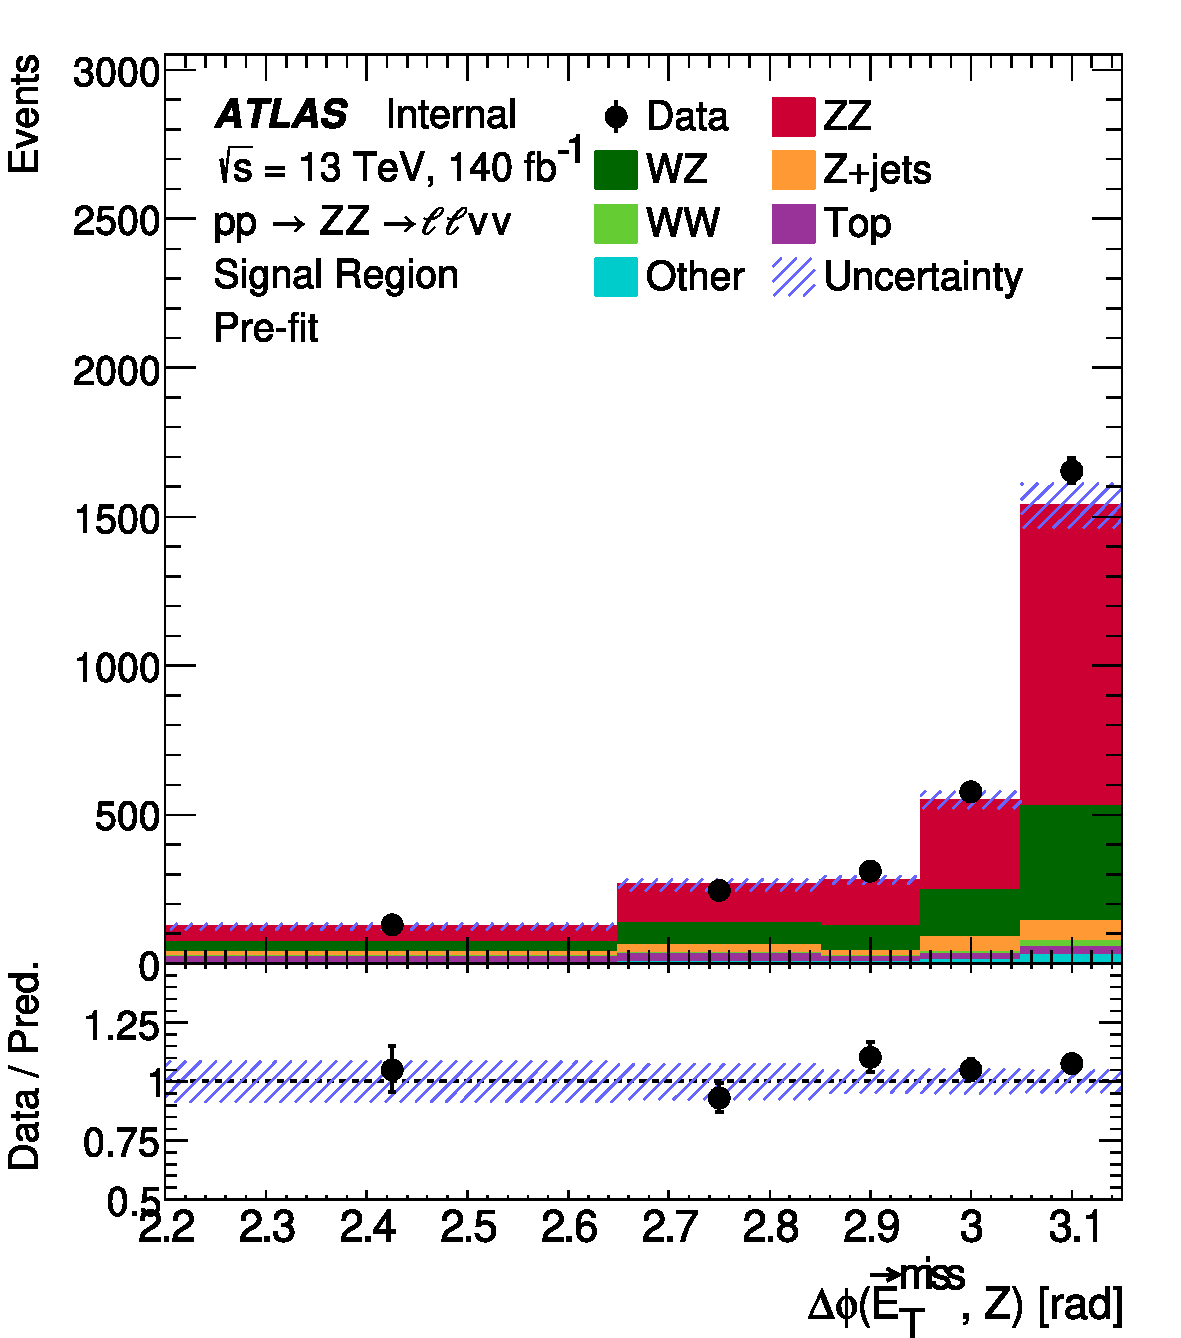
\includegraphics[width=0.45\linewidth]{figures/ch5-llvv/kin-distribution/SignalR-ZZ.pdf}}
    \vspace{0.5cm}
    \subfloat[]{   
    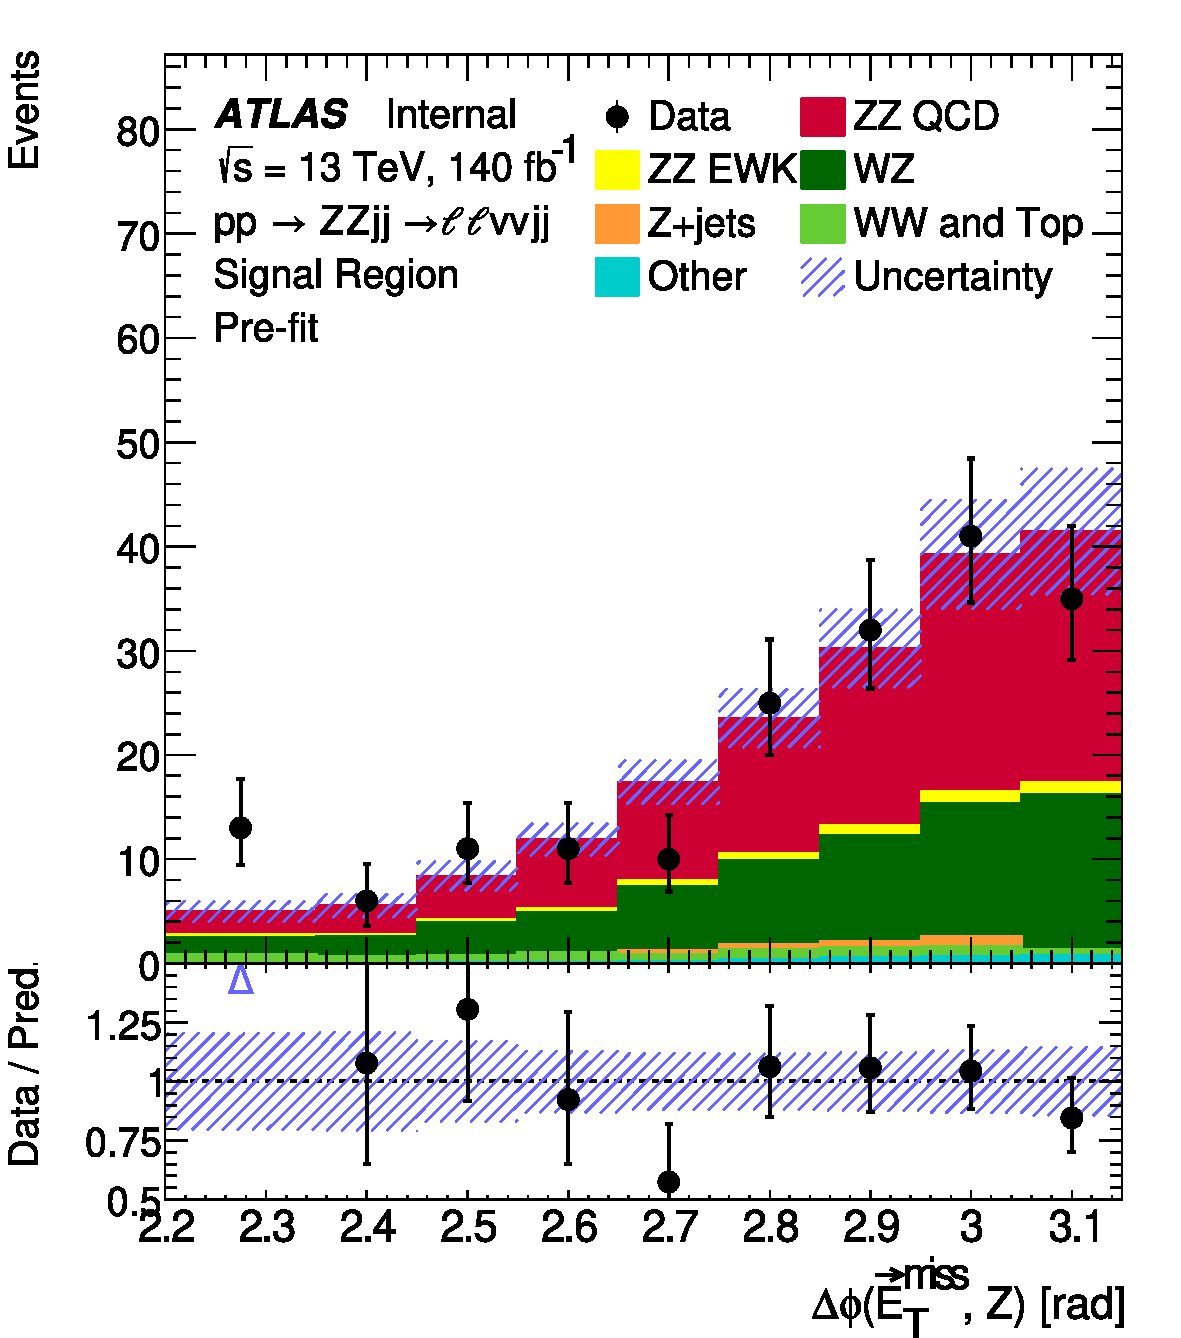
\includegraphics[width=0.45\linewidth]{figures/ch5-llvv/kin-distribution/SignalR-ZZjj.pdf}}
    \caption{Pre-fit comparative analysis between MC predictions and raw data mapping the $\Delta\phi(\vec{E}_{\text{T}}^{\text{miss}}, \text{Z})$ geometry inside the signal regions (SRs): (a) The inclusive $\text{ZZ}$ SR, and (b) The VBS-like $\text{ZZ}jj$ SR.}
    \label{fig:SR-prefit}
\end{figure}

% ======================================================================

%this subsection shall include more comparison and meaning of reco and truth selections. 
\subsubsection{Fiducial Phase Space Definition}
\label{sec:fiducial_definition}

Deriving precise differential and overall cross-sections for $\text{ZZ}$ production represents the core ambition of this analysis. However, raw detector-level observations are inextricably tangled with the acceptance rates of the event filter, which are fundamentally bound by algorithmic efficiencies and the detector's physical geometry. To bypass these hardware biases and deliver data that is directly cross-compatible with pure theoretical frameworks, the entire measurement is locked within a strictly defined \textbf{fiducial phase space}.

Establishing this fiducial boundary serves a dual purpose. Initially, it enforces a model-independent baseline by trapping the measurement strictly within the detector's actual sensory range. This prevents the analysis from heavily leaning on theoretical models to blindly extrapolate data into blind spots, thereby stripping away massive layers of theoretical uncertainty. Concurrently, it sets the necessary mathematical stage for generating the correction factors needed to translate raw detector-level event counts into authentic particle-level collision statistics.

This fiducial territory is mathematically carved out using pure particle-level (``truth'') telemetry sourced from the MC event generators. While these boundaries deliberately shadow the logic of the reconstruction-level filters, they are purposely relaxed. This strategic buffer ensures that the tighter detector-level selection envelope is completely swallowed by the larger fiducial volume. Employing this nested geometry stabilizes the efficiency calculations by virtually eliminating erratic event migrations across the selection borders. Specifically, limits targeting the dilepton invariant mass and missing transverse momentum are notably loosened at the truth level.

\paragraph{\textbf{The MC Truth Object Definitions}}
Prior to mapping the fiducial phase space via particle-level (``truth'') filtering, the underlying MC truth objects are synthesized through the following logic:
\begin{itemize}
    \item \textbf{Dressed Leptons:} To mathematically correct for final-state QED radiation, the four-momenta belonging to any prompt photons located within a tight $\Delta R(\ell, \gamma) < 0.1$ radius of a prompt muon or electron are folded directly into the lepton's baseline four-momentum. This generates ``dressed'' leptons, effectively bridging the gap between theoretical particles and realistic electromagnetic calorimeter measurements.
    \item \textbf{Truth Neutrinos:} The absolute truth missing transverse momentum ($E_{\text{T}}^{\text{miss, truth}}$) is computed by extracting the vector sum magnitude from the combined transverse momenta of every prompt neutrino present in the event.
    \item \textbf{Truth Jets:} Utilizing the anti-$k_t$ algorithm restricted to an $R=0.4$ radius, truth jets are assembled by clustering all stable particles inhabiting the final state (explicitly ignoring all neutrinos and the previously formulated dressed leptons).
\end{itemize}

\paragraph{\textbf{Fiducial Selection for Inclusive Production}}
To map the fiducial volume for the inclusive $\text{ZZ} \to \ell\ell\nu\nu$ cross-section, the truth-level objects must satisfy the following boundaries:
\begin{itemize}
    \item Precisely two dressed leptons of the same-flavour and opposite-sign (SFOS), restricted to $|\eta^\ell| < 2.5$.
    \item Transverse momentum floors demanding $p_{\text{T}}^\ell > 20~\text{GeV}$ for the subleading lepton and $p_{\text{T}}^\ell > 30~\text{GeV}$ for the leading candidate.
    \item A dilepton invariant mass securely positioned within the $76 < m_{\ell\ell} < 106~\text{GeV}$ bracket.
    \item A truth missing transverse momentum vaulting above $E_{\text{T}}^{\text{miss, truth}} > 95~\text{GeV}$.
    \item A strict dilepton angular separation capped at $\Delta R(\ell,\ell) < 1.8$.
    \item A wide azimuthal gap dividing the missing momentum and the dilepton system, requiring $\Delta\Phi(\vec{p}_{\text{T}}^{\,\ell\ell}, \vec{E}_{\text{T}}^{\text{miss, truth}}) > 2.2$.
    \item A scalar ratio dividing the missing momentum by the total transverse momentum exceeding $E_{\text{T}}^{\text{miss, truth}} / H_{\text{T}}^{\text{truth}} > 0.65$.
\end{itemize}

\paragraph{\textbf{Fiducial Selection for VBS-like $\text{ZZ}jj$ Production}}
Targeting the specialized $\text{ZZ}jj \to \ell^+\ell^-\nu\bar{\nu} jj$ cross-section, the fiducial volume imports the inclusive parameters but superimposes strict requirements on hadronic topologies:
\begin{itemize}
    \item Every inclusive fiducial parameter remains active, with the singular exception of the truth missing transverse momentum, which is aggressively raised to $E_{\text{T}}^{\text{miss, truth}} > 130~\text{GeV}$.
    \item The event is mandated to contain a minimum of two truth jets hitting $p_{\text{T}} > 30~\text{GeV}$ within an $|\eta| < 4.5$ envelope.
\end{itemize}

\paragraph{\textbf{Comparison of Detector-Level and Particle-Level Selections}}
To explicitly highlight the geometric relationship separating the ultimate signal regions from their foundational fiducial volumes, Tables~\ref{tab:reco_truth_inclusive} and~\ref{tab:reco_truth_vbs} provide a direct, side-by-side criteria breakdown. The calculated relaxation of the particle-level boundaries—most noticeably across $E_{\text{T}}^{\text{miss}}$ and $m_{\ell\ell}$—is heavily emphasized. This architectural buffer guarantees that standard detector resolution fluctuations cannot artificially bump a large segment of valid signal events outside the fiducial volume, a scenario that would irreparably destabilize the efficiency algorithms.

\begin{table}[!htbp]
    \centering
    \renewcommand{\arraystretch}{1.3}
    \begin{tabular}{l|c|c}
        \hline \hline
        \textbf{Requirement} & \textbf{Detector-Level (Reco)} & \textbf{Particle-Level (Truth)} \\
        \hline
        Leptons & \multicolumn{2}{c}{Exactly 2 SFOS leptons} \\
        Lepton $p_{\text{T}}$ [GeV] & \multicolumn{2}{c}{$> 30$ (lead), $> 20$ (sublead)} \\
        Lepton $|\eta|$ & $< 2.5$ ($\mu$); $< 2.47$ ($e$) & $< 2.5$ ($e, \mu$) \\
        Electron $|\eta|$ Veto & \textbf{Veto $1.37 < |\eta| < 1.52$} & \textbf{Not Applied} \\
        Dilepton Mass ($m_{\ell\ell}$) [GeV] & $80 < m_{\ell\ell} < 100$ & \textbf{$76 < m_{\ell\ell} < 106$} \\
        \hline
        Missing $E_{\text{T}}$ ($E_{\text{T}}^{\text{miss}}$) [GeV] & $> 110$ & \textbf{$> 95$} \\
        Dilepton $\Delta R(\ell,\ell)$ & $< 1.8$ & $< 1.8$ \\
        $\Delta\Phi(\vec{p}_{\text{T}}^{\,\ell\ell}, \vec{E}_{\text{T}}^{\text{miss}})$ & $> 2.2$ & $> 2.2$ \\
        $E_{\text{T}}^{\text{miss}} / H_{\text{T}}$ & $> 0.65$ & $> 0.65$ \\
        \hline
        $b$-Jet Veto & \textbf{Required} & \textbf{Not Applied} \\
        \hline \hline
    \end{tabular}
    \caption{Direct cross-comparison mapping the selection criteria for the \textbf{Inclusive $\text{ZZ}$ Signal Region} at the detector-level (Reco) against its encompassing particle-level (Truth) fiducial volume. Critical deviations are highlighted in \textbf{bold}.}
    \label{tab:reco_truth_inclusive}    
\end{table}

\begin{table}[!htbp]
    \centering
    \renewcommand{\arraystretch}{1.3}
    \begin{tabular}{l|c|c}
        \hline \hline
        \textbf{Requirement} & \textbf{Detector-Level (Reco)} & \textbf{Particle-Level (Truth)} \\
        \hline
        Inclusive Selection Base & Applied & Applied \\
        \hline
        Missing $E_{\text{T}}$ ($E_{\text{T}}^{\text{miss}}$) [GeV] & $> 150$ & \textbf{$> 130$} \\
        Number of Jets ($p_{\text{T}} > 30~\text{GeV}$) & $\geq 2$ & $\geq 2$ \\
        Jet $|\eta|$ &   $< 4.5$ & \textbf{$< 4.5$} \\
        \hline \hline
    \end{tabular}
    \caption{Direct cross-comparison mapping the selection criteria for the \textbf{VBS-like $\text{ZZ}jj$ Signal Region} at the detector-level (Reco) against its encompassing particle-level (Truth) fiducial volume. Structural differences are highlighted in \textbf{bold}.}
    \label{tab:reco_truth_vbs}
\end{table}

The fiducial parameters established here lay the groundwork for extracting the global correction factor, $C$, which mathematically scales the raw detector-level event count into a pure particle-level fiducial yield. Extracted entirely from simulations, this scalar repairs the background-subtracted data by accounting for resolution-driven data migrations and inherent detector blind spots. Mathematically, it is expressed as the ratio comparing the simulated signal events that successfully navigate the rigorous reconstruction-level filter ($N_{\text{Sel}}^{\text{MC}}$) against the volume of simulated signal events that clear the broader particle-level fiducial filter ($N_{\text{fid}}^{\text{MC}}$):
%
\begin{equation}
C = \frac{N_{\text{sel}}^{\text{MC}}}{N_{\text{fid}}^{\text{MC}}} \, .
\end{equation}

Consequently, the definitive fiducial cross-section, $\sigma_{\text{fid}}$, is derived via:
%
\begin{equation}
\sigma_{\text{fid}} = \frac{N_{\text{obs}} - N_{\text{bkg}}}{\mathcal{L}} \cdot \frac{1}{C} \, ,
\end{equation}
%
where $\mathcal{L}$ represents the total integrated luminosity, $N_{\text{bkg}}$ stands for the calculated background noise, and $N_{\text{obs}}$ reflects the sheer number of observed events locked inside the signal region. This structural equation brilliantly isolates the purely hardware-dependent variables ($C$) away from the theory-heavy extrapolations attempting to model the absolute total phase space.

Following this calculation, the correction factor for this specific analysis is anchored at $C = 56.1\%$. This value is synthesized by dividing the final selected MC signal yield by the product of the target integrated luminosity ($140~\text{fb}^{-1}$) and the baseline fiducial cross-section modeled via \textsc{Matrix}.



\section{Background Estimation}
\label{sec:llvv_background}

In the measurement of the $\text{ZZ} \to \ell^+\ell^-\nu\bar{\nu}$ cross-section, several background processes contribute. These can be categorized as follows:

\begin{itemize}

    % --- FIRST TOP-LEVEL ITEM ---
    \item \textbf{Irreducible Backgrounds}
    \begin{itemize}
        \item \textbf{Diboson processes:}
        \begin{itemize}
            \item $\text{WW} \to \ell\nu\ell\nu$: The two neutrinos contribute to the $E_{\text{T}}^{\text{miss}}$ signature, faking the $\text{ZZ} \to \ell\ell\nu\nu$ process.
            \item $\text{WZ} \to \ell\nu\ell\ell$: If one lepton from the $\text{Z}$ is missing in detection, this process could fake the signal.
            \item $\text{ZZ} \to \ell\ell\ell\ell$: If two leptons escape detection, this process contributes as a background.
        \end{itemize}
    \end{itemize}

    % --- SECOND TOP-LEVEL ITEM ---
    \item \textbf{Reducible Backgrounds}
    \begin{itemize}
        \item \textbf{Top-quark backgrounds:}
        \begin{itemize}
            \item $t\bar{t}$: If $b$-jets in the $t\bar{t}$ final states are not tagged properly, it may fake the signal.
            \item Single top ($\text{W}t$): It can contribute similarly to the $t\bar{t}$ background.
        \end{itemize}
        \item \textbf{Drell--Yan + jets} ($\text{Z} \to \ell\ell$ + jets): Jet energy mismeasurement can lead to artificial $E_{\text{T}}^{\text{miss}}$.
        \item \textbf{$\text{W}$ + jets}: A single $\text{W}$ boson decaying leptonically with jets can mimic the signal region due to misidentification of a jet as a faked lepton.
    \end{itemize}

\end{itemize}

To achieve precise cross-section measurements, these backgrounds must be carefully estimated using the background control regions. Considering the final states of the backgrounds, they can be categorized into the following Control Regions (CRs):

\begin{itemize}
    \item \textbf{Non-Resonant Backgrounds} (from $t\bar{t}, \text{W}t, \text{WW}, \tau\tau$):\\
    These processes decay via two $\text{W}$ bosons (or $\tau$ leptons) rather than a $\text{Z}$ boson, resulting in uncorrelated lepton flavors. They are further categorized by $b$-jet multiplicity to separate Top processes from $\text{WW}$ processes:
    \begin{itemize}
        \item \textbf{0 $b$-jet Category ($\text{WW}$ Enriched):}
        \begin{itemize}
            \item $\text{WW} \to \ell\nu\ell\nu$: The dominant contribution in the 0 $b$-tag phase space. The neutrinos create genuine $E_{\text{T}}^{\text{miss}}$.
            \item $t\bar{t}$ / Single Top ($\text{W}t$): Top events contribute to this category only if the $b$-jets fail to be identified (tagging inefficiency) or fall outside detector acceptance.
        \end{itemize}
        \item \textbf{$\ge 1$ $b$-jet Category (Top Enriched):}
        \begin{itemize}
             \item $t\bar{t} \to \text{W}b\text{W}b$ and $\text{W}t$: The dominant contribution when at least one $b$-jet is identified. These events contain real $E_{\text{T}}^{\text{miss}}$ from the $\text{W}$ decays.
        \end{itemize}
    \end{itemize}

    \item \textbf{3-Lepton Backgrounds ($\text{WZ}$)}
    \begin{itemize}
        \item $\text{WZ} \to \ell\nu\ell\ell$: This is an irreducible background if one of the three leptons is lost (fails reconstruction) or falls outside the detector acceptance, mimicking the $2\ell + E_{\text{T}}^{\text{miss}}$ signature.
    \end{itemize}
    
    \item \textbf{$\text{Z}$+Jets Backgrounds (Instrumental $E_{\text{T}}^{\text{miss}}$)}
    \begin{itemize}
        \item \textbf{Drell--Yan + jets} ($\text{Z}/\gamma^* \to \ell\ell$ + jets): The dominant reducible background. It contains real leptons from the $\text{Z}$ boson, but the $E_{\text{T}}^{\text{miss}}$ is artificial (``fake''), caused by jet energy mismeasurement or pile-up interactions.
    \end{itemize}
   
    \item \textbf{Fake Lepton / Instrumental Backgrounds}
    \begin{itemize}
        \item \textbf{$\text{W}$ + jets}: A process with one real lepton from a $\text{W}$ boson and a jet misidentified as a second lepton (fake lepton), creating a fake $2\ell$ signature.
        \item \textbf{Fake $E_{\text{T}}^{\text{miss}}$}: Detector anomalies, cosmic-ray muons, or beam halo effects that produce large artificial missing energy.
    \end{itemize}
\end{itemize}

To accurately estimate background contributions, dedicated control regions (CRs) are defined, each enriched in a specific background process. A simultaneous fit is performed across all CRs and the signal region to constrain both the yields and shapes of these backgrounds consistently. The fit uses event distributions as inputs and derives scale factors that adjust the MC predictions to match the data in the CRs. These scaled MC predictions are then extrapolated to the signal region to provide reliable background estimates, forming the basis for the cross-section measurement.

The following sections describe the estimation strategy for each control region in detail.

\subsection{Non-Resonant Background in $e^\pm\mu^\mp$ CR (With/Without $b$-Jet)}
\label{sec:bkg_emuCR}

Considering the high percentage of the non-resonant backgrounds, it would be better if the control regions are well defined to control the backgrounds from MC estimations. Therefore, 2 Control Regions are defined to further estimate the yields from those processes. 

One is the non-resonant background, which requires different-flavour opposite-sign (DFOS) leptons ($e^\pm\mu^\mp$) in the final state. For example, in the $\text{WW} \to \ell\nu\ell\nu$ process, the observable final state could be either same-flavour opposite-sign (SFOS) leptons, which fakes the true signals, or different-flavour opposite-sign (DFOS) leptons. Considering that there is an equal chance for the $\text{W}$ boson to decay to an electron or muon, the yield ratio between SFOS and DFOS final states would be 1:1 (considering both $ee \ \text{and} \ \mu\mu$ SFOS). Since the DFOS events are well separated from the SFOS, this would be a good approach to estimate the background yields in the Signal Region (SR) using the CR events. 

However, since the final state from top quark pair or single top decay contains 1 or 2 $b$-jets, the observed final state could contain 1 or more $b$-jets. Therefore, define a CR with a 1 $b$-jet to further estimate the yield from top backgrounds. The non-resonant with zero $b$-jet CR definition is the same as the common non-resonant CR, except for the $b$-jet tagging requirement. For the VBS-like $\text{ZZ}jj$ analysis, the non-resonant CR contains both $\text{WW}$ and top background events. 

Since this aims to estimate yields in the SR, the non-resonant background definition is the same as in the SR, except that it requires DFOS events. The detailed definitions of non-resonant with/without 1 $b$-jet are shown in Table~\ref{tab:em_definition}. The pre-fit distributions of $\Delta\phi(\vec{E}_{\text{T}}^{\text{miss}}, \text{Z})$ in the CRs for both data and MC prediction are shown in Figure~\ref{fig:em-CR-prefit}. The purity of the non-resonant background events exceeds 99\% in the CRs.

\begin{table}[!htbp]
\centering
\renewcommand{\arraystretch}{1.2}
\begin{tabular}{|>{\centering\arraybackslash}p{4.5cm}|>{\centering\arraybackslash}p{4.5cm}|}
\hline
\multicolumn{2}{|c|}{Inclusive $\text{ZZ}$ phase space: $t\bar{t}$ / $\text{WW}$ $e\mu$ Control Region cuts} \\
\hline
\multicolumn{2}{|c|}{$80 < m_{\ell\ell} < 100~\text{GeV}$} \\
\hline\multicolumn{2}{|c|}{$E_{\text{T}}^{\text{miss}} > 70~\text{GeV}$} \\
\hline\multicolumn{2}{|c|}{$\Delta R_{\ell\ell} < 2$} \\
\hline\multicolumn{2}{|c|}{$\Delta\phi(\vec{E}_{\text{T}}^{\text{miss}}, \vec{p}_{\text{T}}^{\,e\mu}) > 2.2$} \\
\hline\multicolumn{2}{|c|}{$E_{\text{T}}^{\text{miss}}/H_{\text{T}} > 0.3$} \\
\hline
$b$-jet veto ($\text{WW}$) & $n_{b\text{-jet}} > 0$ (top) \\
\hline
\end{tabular}
\caption{Definition of $t\bar{t}$ / $\text{WW}$ $e\mu$ Control Region in inclusive $\text{ZZ}$ measurement phase-space.}
\label{tab:em_definition}
\end{table}

\begin{figure}[!htbp]
    \centering
    \subfloat[]{
    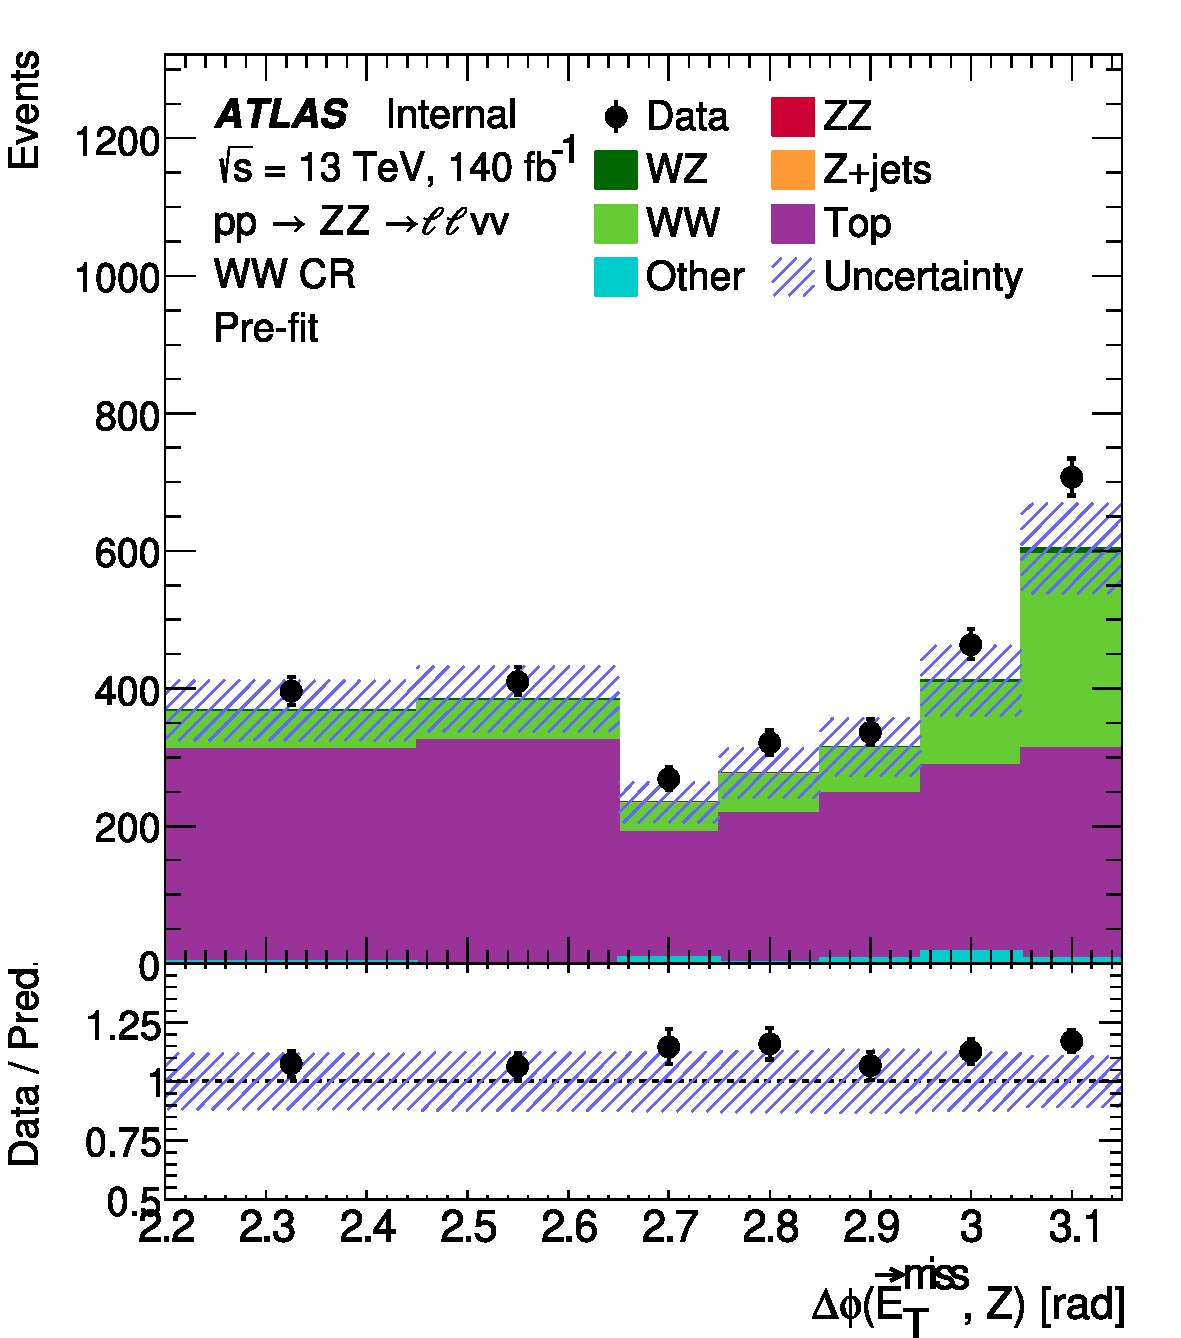
\includegraphics[width=0.32\linewidth]{figures/ch5-llvv/kin-distribution/EMU_A-ZZ.pdf}}
    \subfloat[]{    
    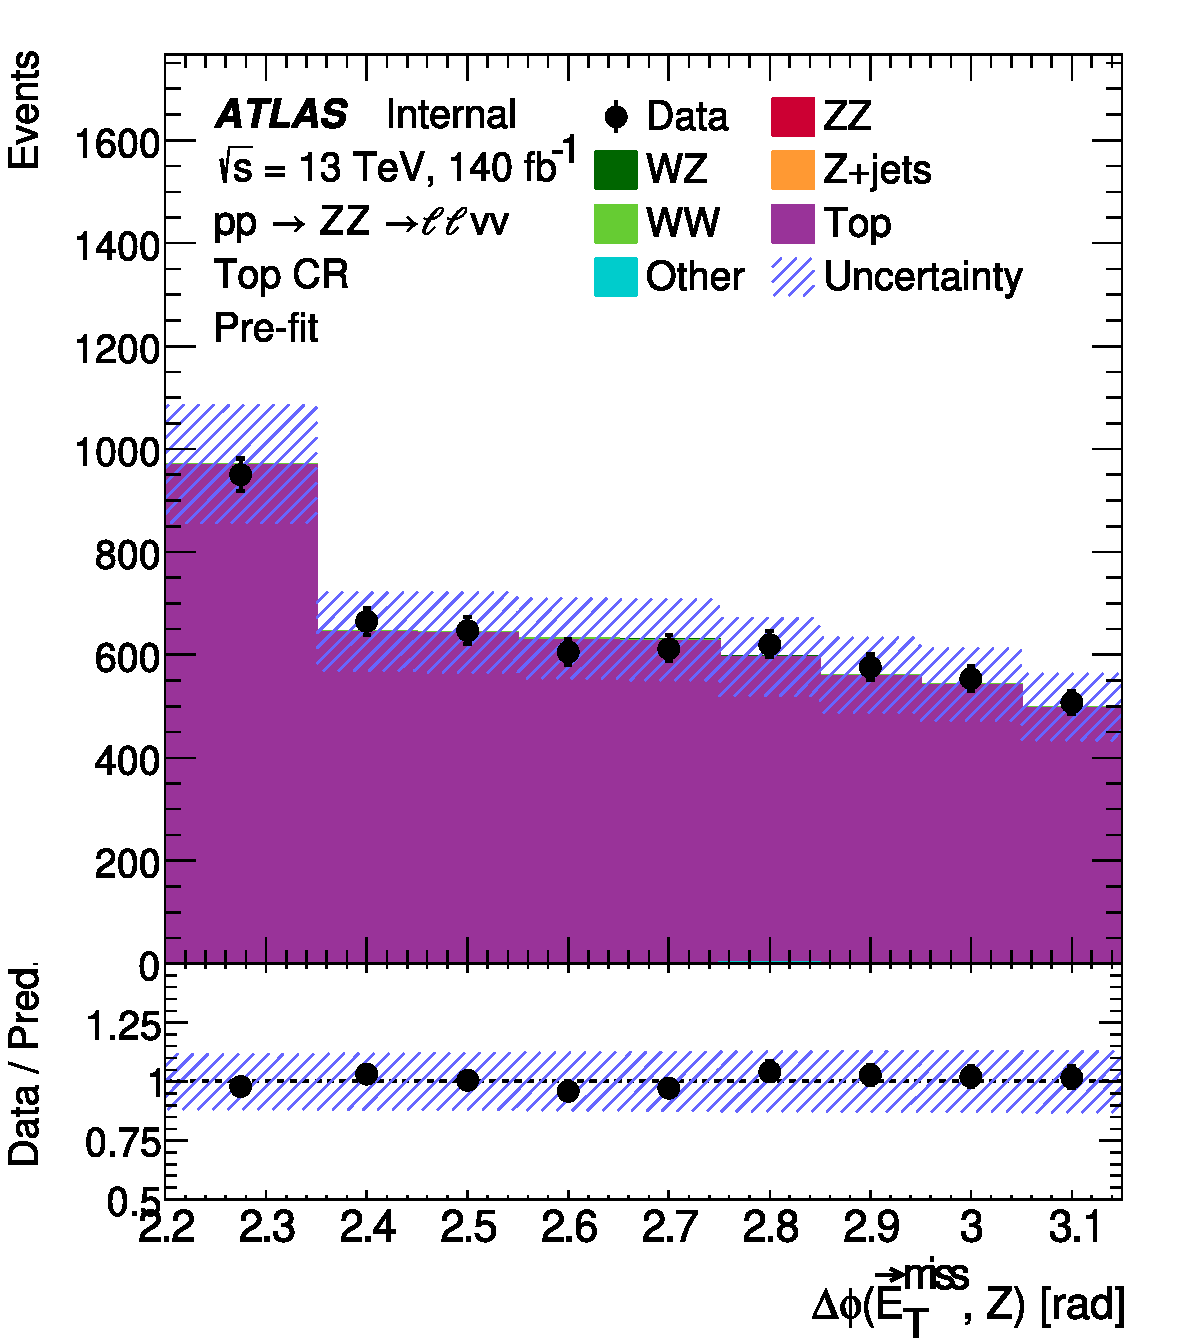
\includegraphics[width=0.32\linewidth]{figures/ch5-llvv/kin-distribution/EMU_B-ZZ.pdf}}
   \subfloat[]{    
    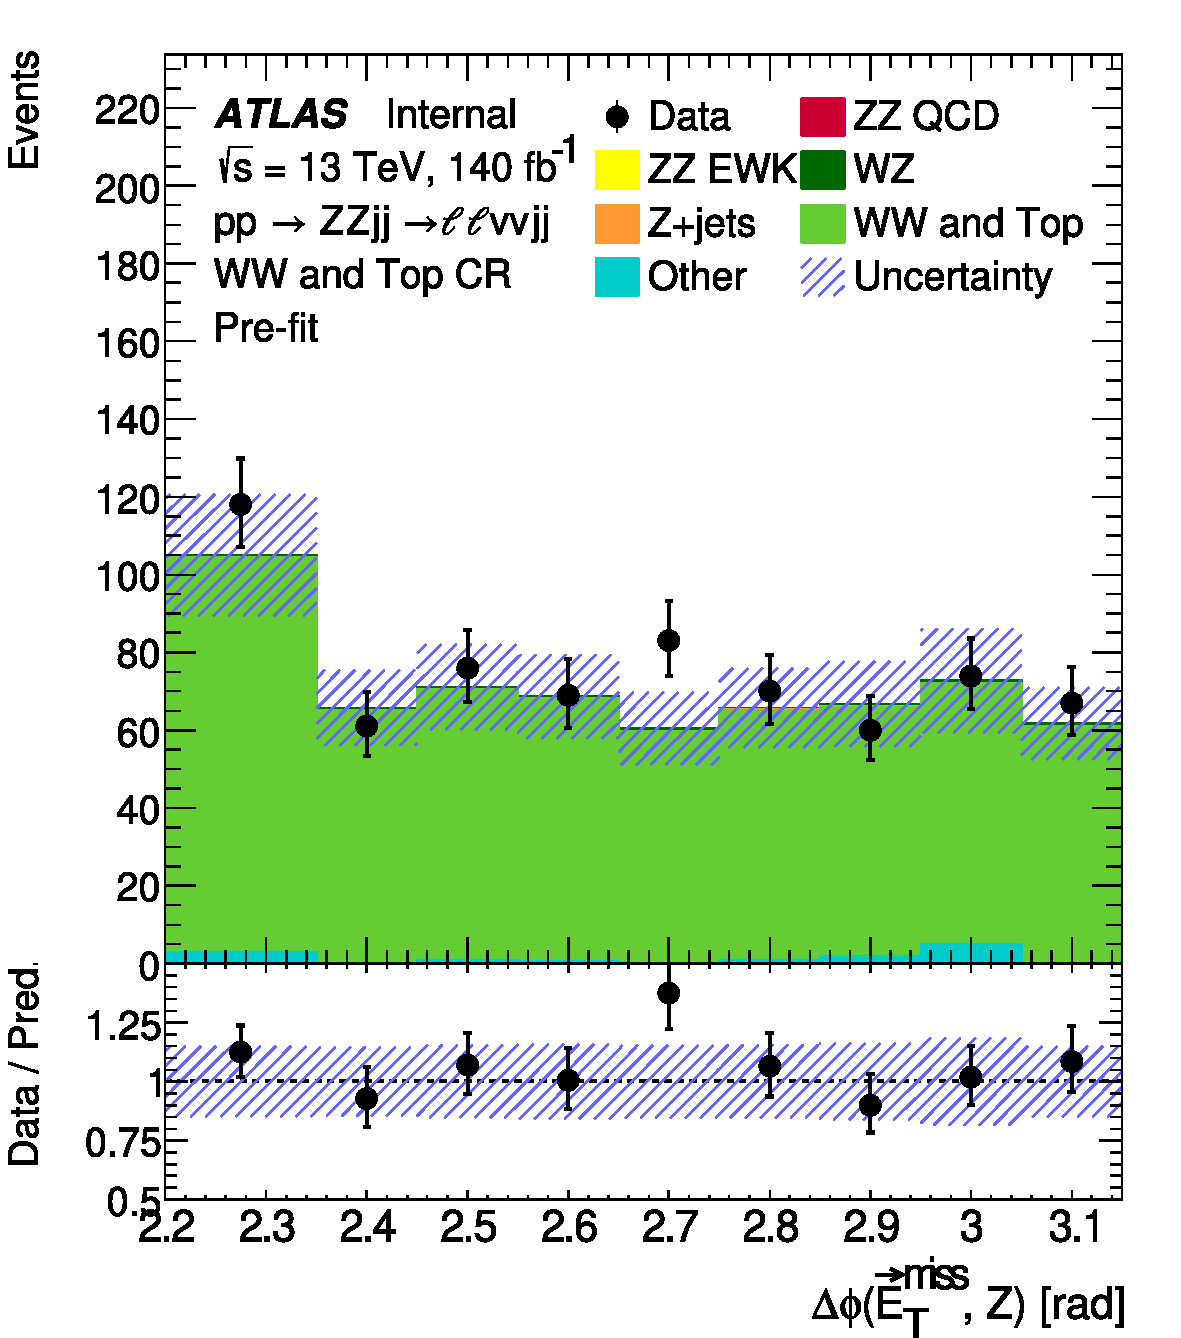
\includegraphics[width=0.32\linewidth]{figures/ch5-llvv/kin-distribution/EMU-ZZjj.pdf}}
    \caption{Data and MC (pre-fit) comparison of the $\Delta\phi(\vec{E}_{\text{T}}^{\text{miss}}, \text{Z})$ in the $e\mu$ CRs for inclusive $\text{ZZ}$ analysis: (a) $\text{WW}$ CR (no $b$-jet), (b) Top CR (with $b$-jets), and (c) for VBS-like $\text{ZZ}jj$ analysis.}
    \label{fig:em-CR-prefit}
\end{figure}

\subsection{3-Lepton Control Region (3$\ell$ CR)}
\label{sec:bkg_3lCR}

The $\text{WZ} \to \ell\nu\ell\ell$ process constitutes a major irreducible background for the $\text{ZZ} \to \ell\ell\nu\nu$ analysis. This process mimics the signal topology if one of the three leptons fails to be reconstructed or falls outside the detector acceptance, resulting in apparent missing transverse energy. To constrain the normalization and modeling of the $\text{WZ}$ background, an inclusive 3-lepton Control Region (3$\ell$ CR) is defined.

\subsubsection{Definition and Event Selection}

The selection criteria for the 3$\ell$ CR are summarized in Table~\ref{table:3lCR_definition_sim}. The primary requirement distinguishing this region from the Signal Region (SR) is the lepton multiplicity; we require the presence of more than two leptons ($n_{\text{leptons}} > 2$). This condition ensures strictly orthogonal phase spaces between the control and signal regions, preventing any event overlap.
\begin{table}[!htbp]
\centering
\begin{tabular}{|l|c|}
\hline
\textbf{Variable} & \textbf{Cut Value} \\ 
\hline 
$n_{\text{leptons}}$ & $> 2$ \\
\hline 
$m_{\ell\ell}$ & $80 < m_{\ell\ell} < 100~\text{GeV}$ \\
\hline 
$E_{\text{T}}^{\text{miss}}$ & $> 70~\text{GeV}$ \\
\hline 
$\Delta R_{\ell\ell}$ & $< 2$ \\ 
\hline 
$\Delta \varphi(E_{\text{T}}^{\text{miss}}, \text{Z})$ & $> 2.2 $ \\
\hline 
$E_{\text{T}}^{\text{miss}} / H_{\text{T}}$ & $> 0.3$ \\
\hline 
Heavy Flavor & $b$-jet veto \\
\hline 
$m_{\text{T, W}}$ & $> 30~\text{GeV}$ \\ 
\hline
\end{tabular}
\caption{Definition of the inclusive 3-lepton Control Region (3$\ell$ CR). The kinematic selections mimic the Signal Region to ensure phase-space compatibility, while the lepton multiplicity ensures orthogonality.}
\label{table:3lCR_definition_sim}
\end{table}

Apart from the lepton multiplicity, the kinematic cuts are chosen to closely mirror those of the Signal Region. This strategy ensures that the control region probes a phase space with similar kinematic characteristics to the signal region, thereby minimizing systematic uncertainties associated with extrapolating the normalization factors (scaling factors) from the CR to the SR. However, certain cuts are kept slightly looser than in the SR to retain higher statistics, reducing the statistical uncertainty on the derived scaling factors.
\begin{figure}[!htbp]
    \centering
    \subfloat[]{
    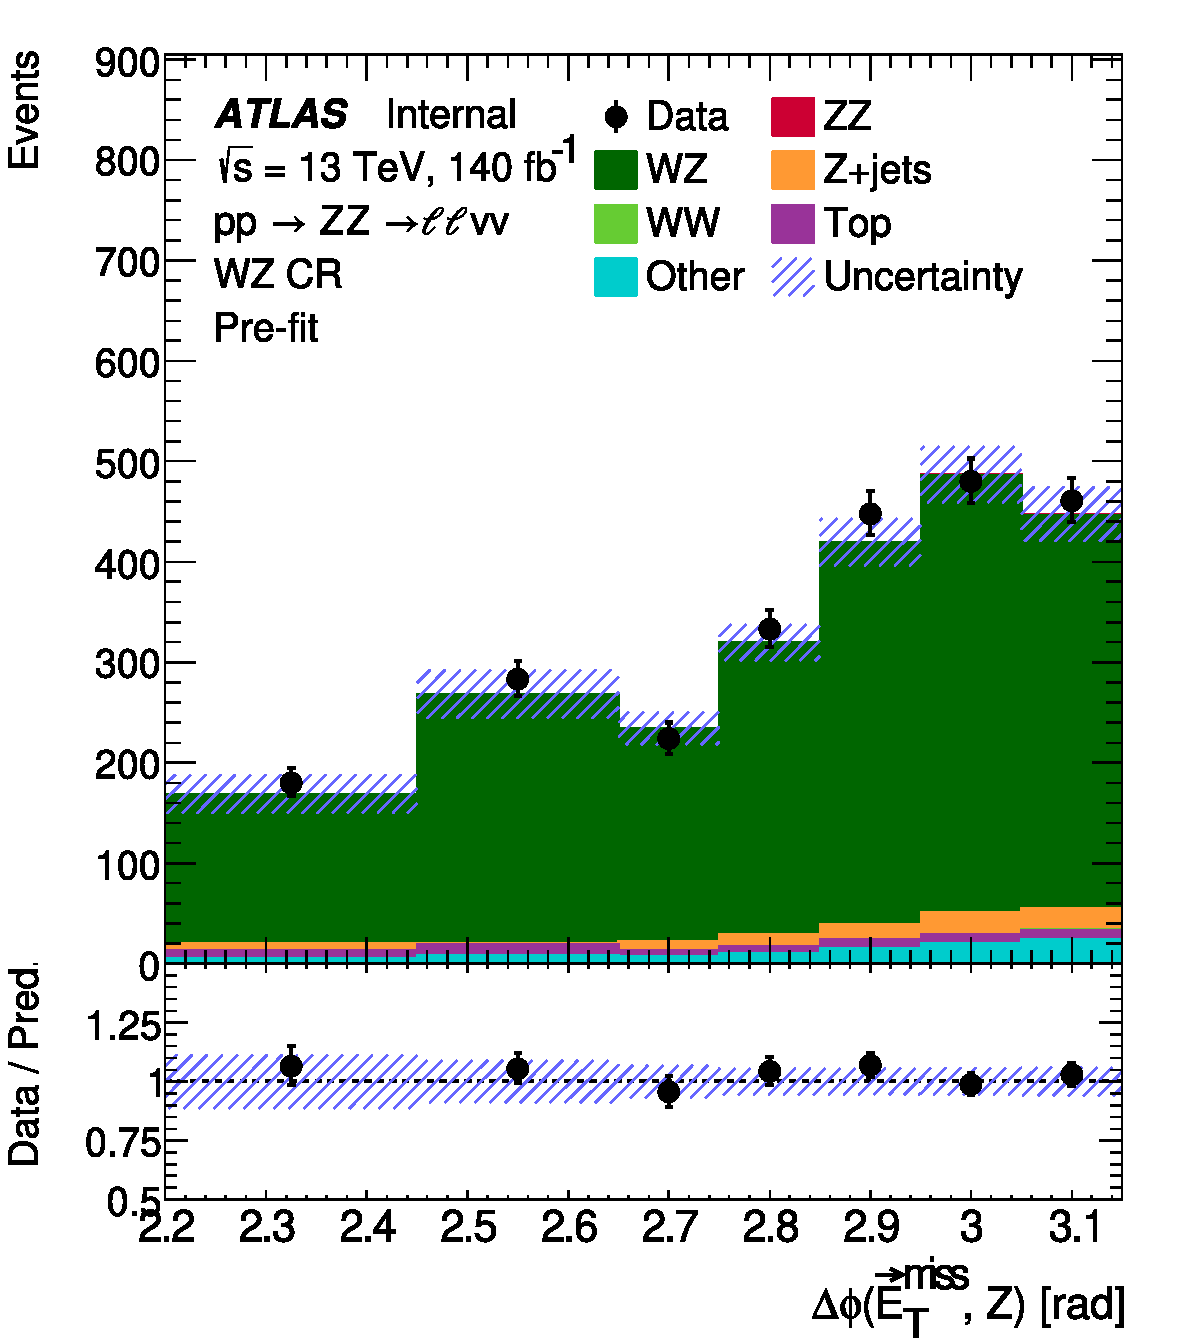
\includegraphics[width=0.45\linewidth]{figures/ch5-llvv/kin-distribution/WZ-ZZ.pdf}}
    \subfloat[]{
    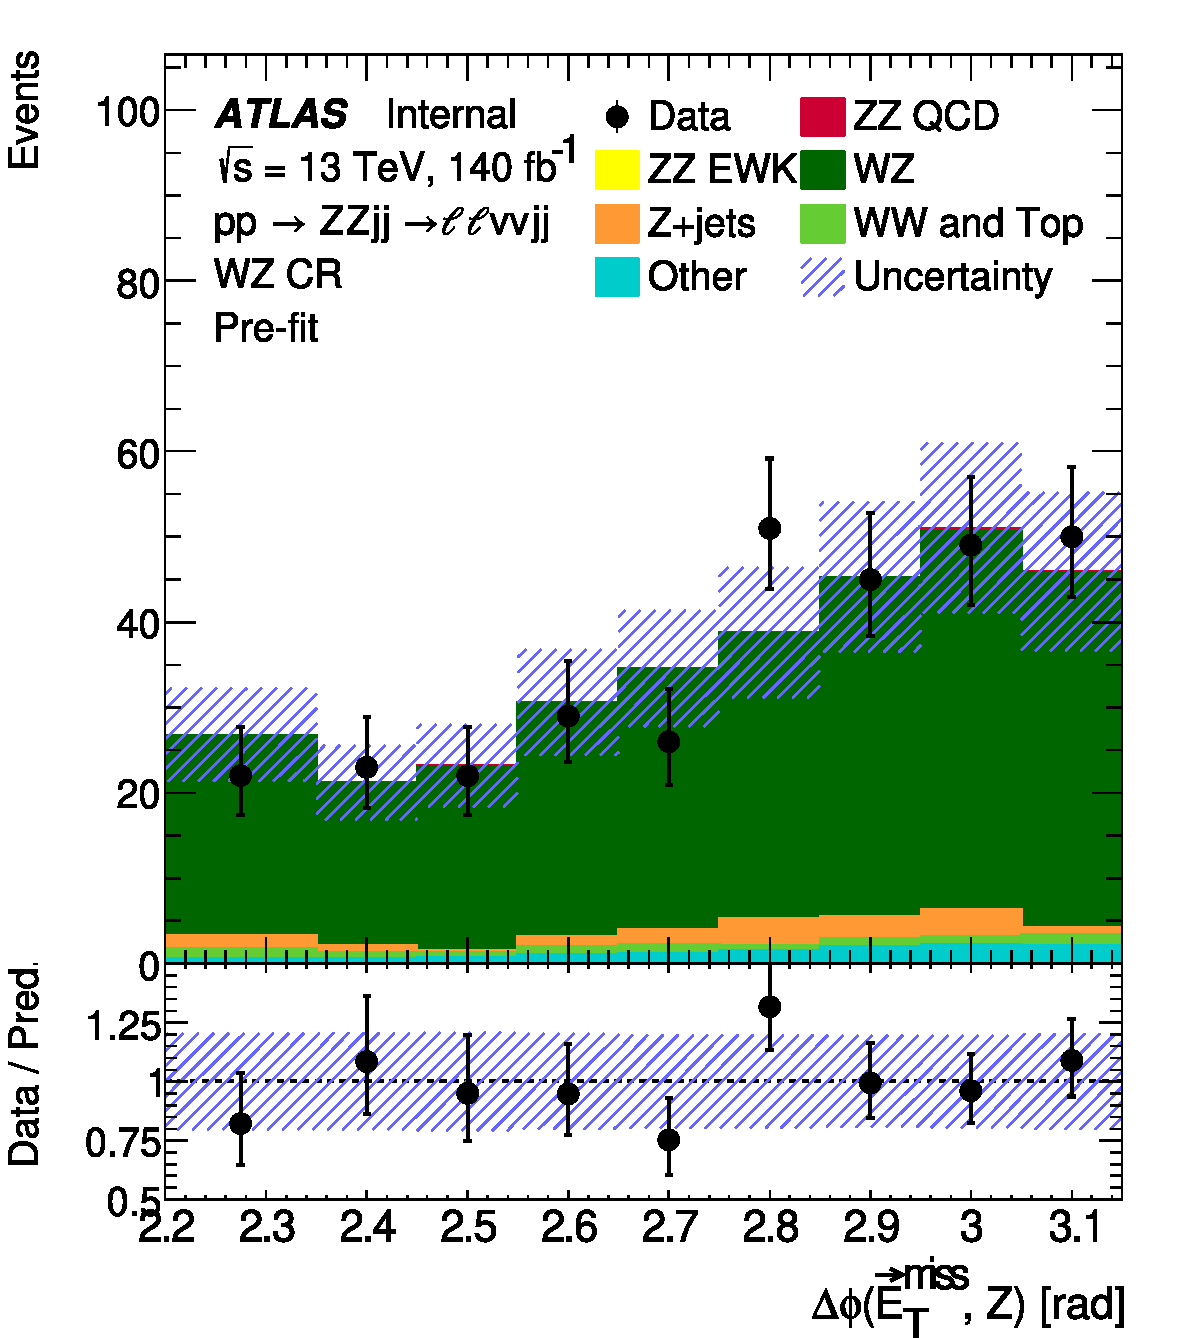
\includegraphics[width=0.45\linewidth]{figures/ch5-llvv/kin-distribution/WZ-ZZjj.pdf}}
    \caption{Data and MC (pre-fit) comparison of the $\Delta\phi(\vec{E}_{\text{T}}^{\text{miss}}, \text{Z})$ in the $\text{WZ}$ 3$\ell$ CR: (a) for the inclusive $\text{ZZ}$ analysis, and (b) for the VBS-like $\text{ZZ}jj$ analysis. }
    \label{fig:3l-CR-prefit}
\end{figure}

Specifically, the selection requires an opposite-sign same-flavour (OSSF) lepton pair consistent with the $\text{Z}$ boson mass ($80 < m_{e\mu} < 100~\text{GeV}$). To select a topology consistent with the high-$p_{\text{T}}$ $\text{Z}$ boson signal, a large missing transverse energy cut ($E_{\text{T}}^{\text{miss}} > 70~\text{GeV}$) and a boost requirement on the leptons ($\Delta R_{\ell\ell} < 2$) are applied.

Furthermore, a transverse mass cut is applied to the third lepton and the $E_{\text{T}}^{\text{miss}}$, denoted as $m_{\text{T, W}} > 30~\text{GeV}$. This cut is introduced specifically to suppress the contribution from $\text{Z}$+jets events where a jet is misidentified as a lepton. By requiring a non-zero $m_{\text{T, W}}$, we reduce the contamination from non-prompt leptons, ensuring high purity of the $\text{WZ}$ process.

The pre-fit distributions of $\Delta\phi(\vec{E}_{\text{T}}^{\text{miss}}, \text{Z})$ for both $\text{ZZ}$ and $\text{ZZ}jj$ analyses in the $\text{WZ}$ 3$\ell$ CR for both data and MC prediction are shown in Figure~\ref{fig:3l-CR-prefit}. The purity of the $\text{WZ}$ background events exceeds 90\% in the CR.

\subsubsection{Composition and Yields}

The pre-fit event yields in the inclusive 3$\ell$ Control Region are presented in Table~\ref{table:3lCR_unscaled}. The region is dominated by the $\text{WZ}$ process, which accounts for approximately 90\% of the total background expectation, confirming the high purity of this control region.
\begin{table}[htbp]
\centering
\resizebox{\textwidth}{!}{%
\begin{tabular}{|l|c|c|c|c|c|}
\hline
\textbf{Process} & \textbf{All Channels} & \textbf{$\mu\mu\mu$} & \textbf{$\mu\mu e$} & \textbf{$\mu ee$} & \textbf{$eee$} \\ \hline
\textbf{Data} & \textbf{2409.0 $\pm$ 49.08} & 639.0 $\pm$ 25.28 & 607.0 $\pm$ 24.64 & 553.0 $\pm$ 23.52 & 610.0 $\pm$ 24.7 \\ \hline
\hline
EWK & 0.1 $\pm$ 0.01 & 0.01 $\pm$ 0.0 & 0.05 $\pm$ 0.01 & 0.04 $\pm$ 0.01 & 0.01 $\pm$ 0.0 \\ \hline
QCD & 2.4 $\pm$ 0.6 & 0.1 $\pm$ 0.13 & 1.47 $\pm$ 0.47 & 0.84 $\pm$ 0.31 & -0.01 $\pm$ 0.17 \\ \hline
\textbf{WZ} & \textbf{2106.3 $\pm$ 11.18} & 582.12 $\pm$ 5.83 & 536.64 $\pm$ 5.71 & 467.68 $\pm$ 5.55 & 519.85 $\pm$ 5.26 \\ \hline
$\text{Z}$+jets & 86.57 $\pm$ 11.0 & 20.56 $\pm$ 5.88 & 20.38 $\pm$ 5.77 & 28.37 $\pm$ 5.1 & 17.25 $\pm$ 5.21 \\ \hline
top, $t\bar{t}\text{V}$, $\text{W}t$ & 57.42 $\pm$ 1.83 & 9.19 $\pm$ 0.68 & 16.2 $\pm$ 0.97 & 18.76 $\pm$ 1.0 & 13.27 $\pm$ 0.97 \\ \hline
$\text{WW}$ & 0.65 $\pm$ 0.14 & 0.03 $\pm$ 0.03 & 0.21 $\pm$ 0.08 & 0.22 $\pm$ 0.08 & 0.2 $\pm$ 0.08 \\ \hline
Rare ($4\ell$, $\text{VVV}$, etc.) & 90.79 $\pm$ 1.35 & 31.86 $\pm$ 1.12 & 15.62 $\pm$ 0.35 & 14.73 $\pm$ 0.35 & 28.58 $\pm$ 0.58 \\ \hline
$\text{ZZ}$ & 2.5 $\pm$ 0.6 & 0.11 $\pm$ 0.0 & 1.52 $\pm$ 0.01 & 0.88 $\pm$ 0.01 & -0.01 $\pm$ 0.0 \\ \hline
\hline
\textbf{Total Bkg} & \textbf{2341.73 $\pm$ 15.85} & 643.85 $\pm$ 8.38 & 590.53 $\pm$ 8.2 & 530.61 $\pm$ 7.62 & 579.14 $\pm$ 7.49 \\ \hline
\hline
Data/MC & 1.03 $\pm$ 0.02 & 0.99 $\pm$ 0.04 & 1.03 $\pm$ 0.04 & 1.04 $\pm$ 0.05 & 1.05 $\pm$ 0.04 \\ \hline
$\frac{\text{Data-nonWZ}}{\text{WZ}}$ & 1.03 $\pm$ 0.03 & 0.99 $\pm$ 0.05 & 1.03 $\pm$ 0.05 & 1.05 $\pm$ 0.06 & 1.06 $\pm$ 0.05 \\ \hline
Signal/$\text{WZ}$ (\%) & 0.12 $\pm$ 0 & 0.02 $\pm$ 0 & 0.28 $\pm$ 0 & 0.19 $\pm$ 0 & -0.0 $\pm$ 0 \\ \hline
\end{tabular}%
}
\caption{Pre-fit event yields in the inclusive 3$\ell$ Control Region. The ``Rare'' category includes $4\ell$, $\ell\ell qq$, $\text{VVV}$, $\text{W}$+jets, and $\text{Z}\tau\tau$. The region is highly pure in $\text{WZ}$ events.}
\label{table:3lCR_unscaled}
\end{table}

The data generally shows good agreement with the Monte Carlo predictions even before the simultaneous fit. The ratio of Data to MC is found to be $1.03 \pm 0.02$ for the inclusive channel. The contamination from the signal process ($\text{ZZ} \to 2\ell2\nu$) in this region is negligible ($\approx 0.12\%$ relative to the $\text{WZ}$ yield), ensuring that the normalization of the background can be constrained without significant bias from the signal.


\subsection{$\text{Z}$+Jets Control Region ($\text{Z}$+Jets CR)}
\label{sec:bkg_ZjetsCR}

The estimation of the $\text{Z}$+jets background presents a unique challenge in the $\text{ZZ} \to \ell\ell\nu\nu$ analysis. Unlike the irreducible diboson backgrounds, the missing transverse energy in $\text{Z}$+jets events is instrumental (``fake''), arising primarily from jet energy mismeasurement, pile-up interactions, and detector resolution effects rather than from genuine neutrinos. Consequently, the modeling of $E_{\text{T}}^{\text{miss}}$ in Monte Carlo simulations is highly sensitive to the accuracy of the detector response, jet energy corrections, and track reconstruction.

\subsubsection{Definition and Event Selection}

To constrain this background using data, a Control Region must be defined that is rich in $\text{Z}$+jets events while maintaining orthogonality to the Signal Region. This creates a tension in the selection logic:
\begin{itemize}
    \item \textbf{Similarity:} The CR should probe high $E_{\text{T}}^{\text{miss}}$ and high $E_{\text{T}}^{\text{miss}}/H_{\text{T}}$ values to resemble the kinematic phase space of the Signal Region.
    \item \textbf{Purity:} The CR must have minimal contamination from true $\text{ZZ} \to 2\ell2\nu$ signal events to ensure independent background estimation.
    \item \textbf{Orthogonality:} The specific cut values must ensure no overlap with the Signal Region.
\end{itemize}

To satisfy these requirements, the $\text{Z}$+jets CR is defined using a two-dimensional selection in the ($E_{\text{T}}^{\text{miss}}$, $E_{\text{T}}^{\text{miss}}/H_{\text{T}}$) plane, selecting events that fall just outside the signal boundaries. The specific selection logic is:
\begin{equation}
\small
\left( 70 < E_{\text{T}}^{\text{miss}} < 80~\text{GeV} \land \frac{E_{\text{T}}^{\text{miss}}}{H_{\text{T}}} > 0.3 \right) 
\lor 
\left( E_{\text{T}}^{\text{miss}} > 80~\text{GeV} \land 0.3 < \frac{E_{\text{T}}^{\text{miss}}}{H_{\text{T}}} < 0.45 \right)
\end{equation}

This definition captures the tail of the $\text{Z}$+jets distribution that is kinematically closest to the signal. The geometric relationship between the Signal Region and the $\text{Z}$+jets Control Region in this phase space is illustrated in Figure~\ref{fig:Zjets_Control_Region}.

\begin{figure}[!htbp]
 \centering
 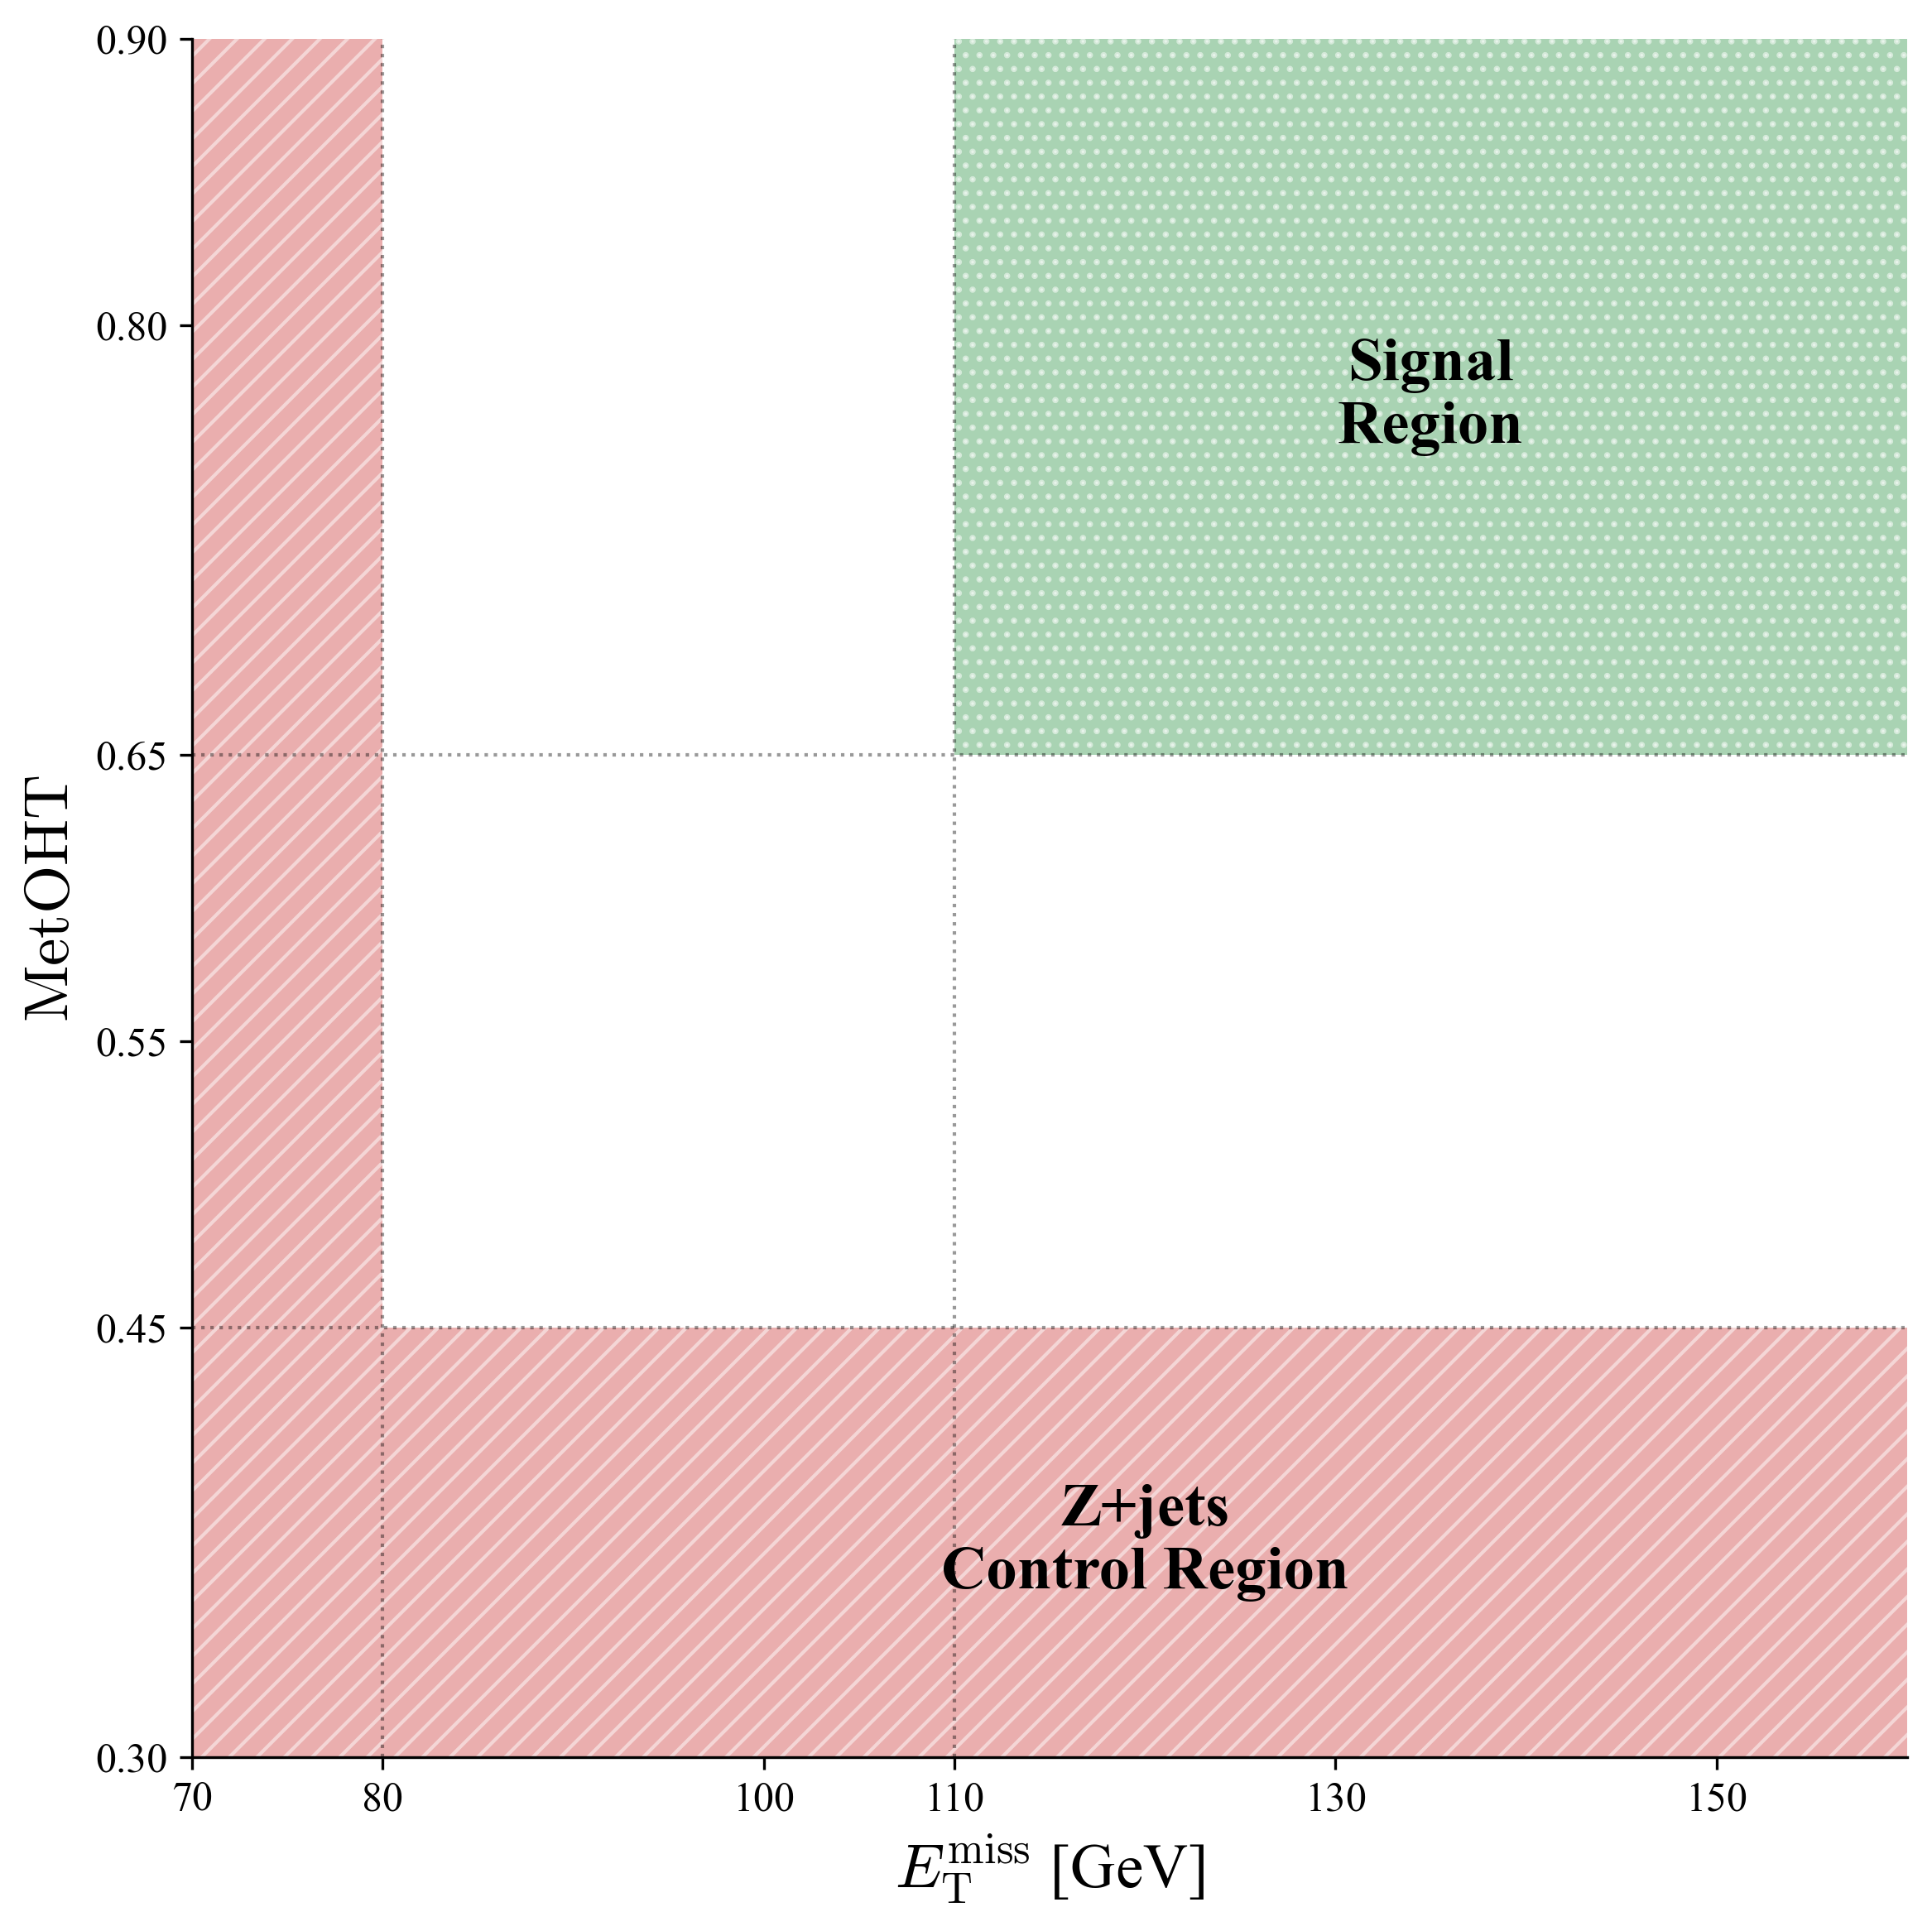
\includegraphics[width=0.6\textwidth]{figures/ch5-llvv/Zjets_Control_Region.png}
 \caption{Illustration of the inclusive phase-space in the ($E_{\text{T}}^{\text{miss}}$, $E_{\text{T}}^{\text{miss}}/H_{\text{T}}$) plane. The $\text{Z}$+jets Control Region is defined to be adjacent to the Signal Region to constrain the fake $E_{\text{T}}^{\text{miss}}$ tail while maintaining orthogonality.}
 \label{fig:Zjets_Control_Region}
\end{figure}

All other kinematic selections, such as the dilepton mass window ($80 < m_{\ell\ell} < 100~\text{GeV}$), lepton separation ($\Delta R_{\ell\ell} < 1.8$), and azimuthal separation ($\Delta \varphi(E_{\text{T}}^{\text{miss}}, \text{Z}) > 2.2$), are kept identical to the Signal Region to minimize extrapolation uncertainties. A summary of the cuts is provided in Table~\ref{table:Zjets_definition}.


\begin{table}[!htbp]
\centering
\begin{tabular}{|l|c|}
\hline
\textbf{Variable} & \textbf{Cut Value} \\ 
\hline 
Dilepton Mass & $80 < m_{\ell\ell} < 100~\text{GeV}$ \\
\hline 
\multirow{2}{*}{$E_{\text{T}}^{\text{miss}}$ / Significance} & ($70 < E_{\text{T}}^{\text{miss}} < 80~\text{GeV}$ \textbf{and} $E_{\text{T}}^{\text{miss}} / H_{\text{T}} > 0.3$) \\
& \textbf{OR} ($E_{\text{T}}^{\text{miss}} > 80~\text{GeV}$ \textbf{and} $0.3 < E_{\text{T}}^{\text{miss}} / H_{\text{T}} < 0.45$) \\
\hline 
Lepton separation & $\Delta R_{\ell\ell} < 1.8$ \\ 
\hline 
Azimuthal separation & $\Delta \varphi(E_{\text{T}}^{\text{miss}}, \text{Z}) > 2.2 $ \\
\hline 
Heavy Flavor & $b$-jet veto \\
\hline
\end{tabular}
\caption{Definition of the inclusive $\text{Z}$+jets Control Region. The region targets the phase space dominated by instrumental $E_{\text{T}}^{\text{miss}}$ while remaining orthogonal to the signal region.}
\label{table:Zjets_definition}
\end{table}

\subsubsection{Categorization by Jet Multiplicity}

Studies of the $\text{Z}$+jets modeling revealed significant shape differences between Data and Monte Carlo in key distributions used for unfolding. Since the fake $E_{\text{T}}^{\text{miss}}$ originates largely from jet mismeasurements, the kinematics of the event are strongly correlated with the number of hadronic jets. 

It was determined that a single global scaling factor was insufficient to correct the $\text{Z}$+jets prediction across the entire phase space. Therefore, the control region is split into three sub-regions based on jet multiplicity ($n_{\text{jets}}$):
\begin{itemize}
    \item $n_{\text{jets}} = 0$
    \item $n_{\text{jets}} = 1$
    \item $n_{\text{jets}} \ge 2$
\end{itemize}
Independent scaling factors are derived for each of these bins during the simultaneous fit. While a finer binning was investigated (separating $n_{\text{jets}}=2$ and $n_{\text{jets}} \ge 3$), results indicated that the scaling behavior was consistent for higher jet multiplicities, justifying the merged $\ge 2$ bin.

The pre-fit distributions of data and MC predictions in the $\text{Z}$+jets control regions (CRs) with three jet multiplicity categories are shown in Figure~\ref{fig:Zjet-CR} for the inclusive $\text{ZZ}$ analysis. The purity of $\text{Z}$+jets background events exceeds 95\% in these CRs. Although the observed data yields are higher than the MC predictions, they remain consistent within the associated uncertainties. In the final cross-section measurement, the normalization of the MC prediction will be determined through a simultaneous fit, which constrains the background contributions to the signal region.
For the VBS-like analysis, the $\text{Z}$+jets background is estimated using MC simulation due to the very limited statistics available in the $\text{ZZ}jj$ phase space. A conservative normalization uncertainty is assigned to this background in the fit to the $\text{ZZ}jj$ cross-section.

\begin{figure}[!htbp]
    \centering
    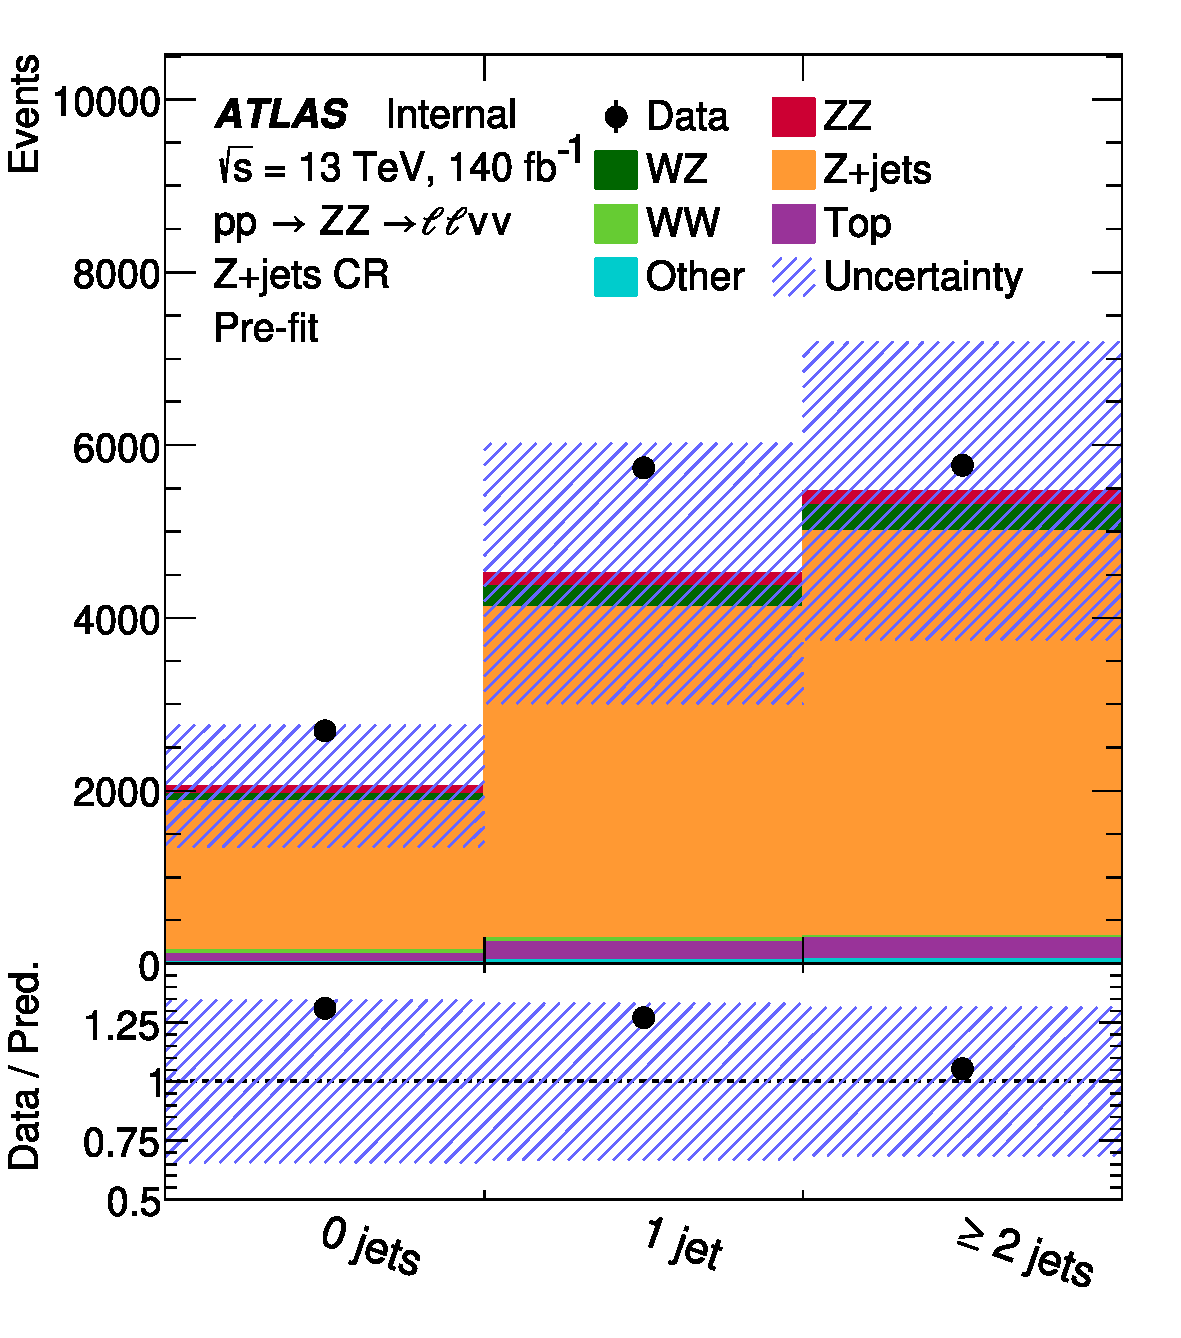
\includegraphics[width=0.5\linewidth]{figures/ch5-llvv/kin-distribution/Zj_VR_nJ-ZZ.pdf}
    \caption{Data and MC (pre-fit) comparison of the $\Delta\phi(\vec{E}_{\text{T}}^{\text{miss}}, \text{Z})$ in the $\text{Z}$+Jets CRs.}
    \label{fig:Zjet-CR}
\end{figure}

\subsubsection{Composition and Yields}

The pre-fit event yields for the inclusive $\text{Z}$+jets Control Region are detailed in Table~\ref{table:Zjets_unscaled}. 
\begin{table}[htbp]
\centering
\resizebox{\textwidth}{!}{%
\begin{tabular}{|l|c|c|c|}
\hline
\textbf{Process} & \textbf{$ee$ and $\mu\mu$} & \textbf{$ee$} & \textbf{$\mu\mu$} \\ \hline
\textbf{Data} & \textbf{14193.0 $\pm$ 119.13} & 6841.0 $\pm$ 82.71 & 7352.0 $\pm$ 85.74 \\ \hline
\hline
EWK & 11.62 $\pm$ 0.1 & 5.7 $\pm$ 0.07 & 5.92 $\pm$ 0.07 \\ \hline
QCD & 397.1 $\pm$ 5.98 & 183.28 $\pm$ 3.99 & 213.82 $\pm$ 4.45 \\ \hline
$\text{WZ}$ & 636.46 $\pm$ 7.49 & 301.33 $\pm$ 3.88 & 335.13 $\pm$ 6.41 \\ \hline
\textbf{$\text{Z}$+jets} & \textbf{10239.25 $\pm$ 176.43} & 4712.74 $\pm$ 120.55 & 5526.52 $\pm$ 128.83 \\ \hline
top, $t\bar{t}\text{V}$, $\text{W}t$ & 535.95 $\pm$ 5.94 & 262.62 $\pm$ 4.16 & 273.33 $\pm$ 4.24 \\ \hline
$\text{WW}$ & 113.04 $\pm$ 1.89 & 51.64 $\pm$ 1.28 & 61.4 $\pm$ 1.39 \\ \hline
Rare ($4\ell$, $\text{VVV}$, etc.) & 104.46 $\pm$ 4.38 & 54.65 $\pm$ 4.22 & 49.81 $\pm$ 1.19 \\ \hline
$\text{ZZ}$ & 408.72 $\pm$ 5.98 & 188.98 $\pm$ 3.99 & 219.74 $\pm$ 3.99 \\ \hline
\hline
\textbf{Total Bkg} & \textbf{11629.16 $\pm$ 176.76} & 5382.98 $\pm$ 120.77 & 6246.19 $\pm$ 129.07 \\ \hline
\hline
Data/MC & 1.18 $\pm$ 0.02 & 1.23 $\pm$ 0.03 & 1.14 $\pm$ 0.03 \\ \hline
$\frac{\text{Data-OtherBkg}}{\text{Zjets}}$ & 1.21 $\pm$ 0.03 & 1.27 $\pm$ 0.05 & 1.16 $\pm$ 0.05 \\ \hline
Signal/$\text{Z}$+jets (\%) & 3.99 $\pm$ 0 & 4.01 $\pm$ 0 & 3.98 $\pm$ 0 \\ \hline
\end{tabular}%
}
\caption{Pre-fit event yields in the inclusive $\text{Z}$+jets Control Region. The last row indicates the ratio of the Signal expectation to the dominant $\text{Z}$+jets background, confirming the region is background-enriched.}
\label{table:Zjets_unscaled}
\end{table}

The control region is dominated by $\text{Z}$+jets events, but shows a significant normalization discrepancy pre-fit, with Data exceeding the MC prediction by approximately 18\% in the inclusive selection. This reinforces the necessity of the data-driven scaling factors derived from this region. The signal contamination is controlled at the level of $\approx 4\%$.

%Validation of the simultaneous fit performance across these regions is detailed in Appendix~\ref{sec:TestScaled_3lCR}, while systematic uncertainties associated with the control region definitions and scaling factors are discussed in Section~\ref{sec:SystScaleFactorsCRvariations}.


\subsection{Minor Backgrounds}
\label{sec:bkg_minor}

Several background processes contribute to the signal region at a subleading level (typically $< 1\%$ of the total yield). Due to their small cross-sections or low acceptance in the analysis phase space, it is not feasible to define statistically significant dedicated control regions for these processes. Instead, their contributions are estimated purely from MC simulations normalized to their theoretical cross-sections.

These minor backgrounds include:

\begin{itemize}
    \item \textbf{$\text{ZZ} \to 4\ell$:} This process can enter the signal region if two leptons are lost (e.g., falling outside detector acceptance or failing identification). While physically similar to the signal, the requirement of large $E_{\text{T}}^{\text{miss}}$ strongly suppresses this contribution.
    
    \item \textbf{Triboson Production ($\text{VVV}$):} Processes such as $\text{WWW}$, $\text{WWZ}$, and $\text{WZZ}$ have very small production cross-sections but can produce high lepton multiplicities and missing energy.
    
    \item \textbf{$t\bar{t}\text{V}$ ($t\bar{t}\text{Z}$, $t\bar{t}\text{W}$):} Associated production of top pairs with a boson. These events are largely rejected by the $b$-jet veto applied in the signal region.
    
    \item \textbf{$\text{W}$ + jets:} Events where a $\text{W}$ boson decays leptonically and a jet is misidentified as a second lepton. Strict lepton identification and isolation criteria employed in this analysis reduce this background to a negligible level.
\end{itemize}

Since these backgrounds are not constrained by data in the simultaneous fit, conservative systematic uncertainties are assigned to their theoretical cross-sections (typically on the order of $20\%$ to $30\%$) to account for potential modeling discrepancies.

\subsection{Summary of the Data and MC Yields from SRs and CRs}
\label{sec:summary-table}

Data and pre-fit MC yields for the inclusive $\text{ZZ}$ phase space are presented in Table~\ref{tab:prefitYieldsInclu}. The predicted signal-to-background ratio in the signal region (SR) is approximately 1.5. The targeted background control regions exhibit high purity: for example, the top-quark purity in the non-resonant CR with a $b$-jet requirement is close to 100\%, while the $\text{WZ}$ purity in the $\text{WZ}$ CR exceeds 90\%.


\begin{table}[htbp]
    \centering
    \renewcommand{\arraystretch}{1.2}
    \resizebox{\textwidth}{!}{%
    \begin{tabular}{lccccccc}
       \hline
\textbf{Process} & \textbf{SR} & \textbf{$\text{WZ}$ CR} & \textbf{$\text{WW}$ CR} & \textbf{Top CR}
& \textbf{$\text{Z}$+0j CR} & \textbf{$\text{Z}$+1j CR} & \textbf{$\text{Z}+\ge 2\text{j}$ CR} \\
       \hline
        $\text{ZZ}$ signal     & 1650 (36)    & 2.6 (0.7)    & 0.58 (0.11)  & 0.005 (0.011) & 100 (12)     & 150 (20)      & 160 (34)      \\
        \hline \hline
        \textbf{Background} &  & & & & & & \\
        \hline
        $\text{WZ}$            & 740 (43)     & 2100 (140)   & 22 (2)       & 0.9 (0.3)    & 80 (12)      & 250 (28)      & 310 (60)      \\
        $\text{Z}$+0j          & 80 (34)      & 40 (17)      & 0.6 (1.0)    & 0            & 1700 (670)   & 0             & 0             \\
        $\text{Z}$+1j          & 80 (40)      & 40 (14)      & 2.2 (0.7)    & 0.12 (0.08)  & 0            & 3800 (1460)   & 0             \\
        $\text{Z}+\ge 2\text{j}$ & 13 (7)       & 20 (12)      & 0.4 (0.6)    & 0.15 (0.16)  & 0            & 0             & 4700 (1700)   \\
        $\text{WW}$            & 36.2 (1.9)   & 0.65 (0.12)  & 672 (41)     & 13.9 (1.6)   & 48 (6)       & 46 (5)        & 18.5 (1.9)    \\
        Top                    & 114 (20)     & 57 (8)       & 1850 (290)   & 5700 (710)   & 92 (25)      & 200 (39)      & 250 (43)      \\
        Other                  & 48 (4)       & 91 (7)       & 46 (13)      & 3.4 (1.3)    & 12 (3)       & 44 (10)       & 48 (10)       \\
       \hline
        Total prediction       & 2760 (120)   & 2340 (150)   & 2590 (310)   & 5720 (710)   & 2050 (700)   & 4510 (1500)   & 5470 (1700)   \\
        \hline \hline
        \textbf{Data}          & \textbf{2917} & \textbf{2409} & \textbf{2903} & \textbf{5736} & \textbf{2691} & \textbf{5733} & \textbf{5769} \\
       \hline
    \end{tabular}}
    \caption{Data and pre-fit MC yields for the inclusive $\text{ZZ}$ phase-space. The ``Other'' category includes events from the processes $\text{ZZ} \to 4\ell, 2\ell 2q$, $\text{VVV}~(\text{V}=\text{W,Z})$, $\text{W}j$, $\text{Z} \to \tau\tau$, and $\text{WH}$. The selected number of data events in the SR and the CRs is also provided. The numbers shown in the parentheses are the MC uncertainties.}
    \label{tab:prefitYieldsInclu}    
\end{table}

Data and pre-fit MC yields for the VBS-like $\text{ZZ}jj$ phase space are presented in Table~\ref{tab:prefitYieldsZZjj}. The predicted signal-to-background ratio in the signal region (SR) is approximately 1.45. The overall Top+$\text{WW}$ purity in the non-resonant CR is 97\%, while the $\text{WZ}$ purity in the $\text{WZ}$ CR is 88\%.


\begin{table}[htbp]
    \centering
    \small
    \renewcommand{\arraystretch}{1.2}
    \begin{tabular}{lccc}
       \hline
\textbf{Process} & \textbf{SR} & \textbf{$\text{WZ}$ CR} & \textbf{$\text{WW}$ and Top CR} \\
       \hline
        $\text{ZZ}$ signal     & 108 (12)   & 1.0 (0.3)  & 0.006 (0.004) \\
        \hline
        \hline
        \textbf{Background} &  & &  \\
        \hline        
        $\text{WZ}$            & 62 (12)    & 280 (60)   & 4.8 (1.0)     \\
        $\text{Z}$+jets        & 2.4 (1.2)  & 15 (8)     & 0.4 (0.2)     \\
        $\text{WW}$ and Top    & 7.2 (1.5)  & 8.2 (1.8)  & 620 (90)      \\
        Other                  & 3.0 (0.7)  & 12 (3)     & 12 (14)       \\
       \hline
        Total prediction       & 183 (21)   & 320 (60)   & 640 (100)     \\
        \hline \hline
       \textbf{Data}           & \textbf{184} & \textbf{317} & \textbf{678} \\
       \hline
    \end{tabular}
    \caption{Data and pre-fit MC yields for the $\text{ZZ}jj$ phase-space. The ``Other'' category includes events from the processes $\text{ZZ} \to 4\ell, 2\ell 2q$, $\text{VVV}~(\text{V}=\text{W,Z})$, $\text{W}j$, $\text{Z} \to \tau\tau$, and $\text{WH}$ production. The selected number of data events in the SR and the CRs is also provided in the table. The numbers shown in the parentheses are the MC uncertainties.}
    \label{tab:prefitYieldsZZjj}
\end{table}



\section{Systematic Uncertainties}
\label{sec:llvv_systematics}

This section summarizes the experimental and theoretical sources of systematic uncertainty affecting the event yields of both the signal and background processes, and their impact on the total and differential cross-section measurements.

The systematic uncertainties are evaluated to account for residual discrepancies between data and simulation in the modelling of trigger efficiencies, lepton reconstruction and identification, jet calibration, $b$-tagging, missing transverse energy ($E_{\text{T}}^{\text{miss}}$), the integrated luminosity, and the average number of proton--proton interactions per bunch crossing (pile-up). In addition, theoretical uncertainties are considered, including those arising from the choice of parton distribution functions, renormalization and factorization scales, higher-order corrections, and the modelling of parton shower and hadronization.

Consistent with previous analyses of the $\text{ZZ}jj$ final state, the measurement of the signal yields and the resulting cross-sections is dominated by statistical uncertainty. Among the systematic sources, the largest contributions arise from jet reconstruction, particularly pile-up suppression and $\eta$-intercalibration, as well as from the unfolding procedure.
%The bias associated with the unfolding method is evaluated through the data-driven closure test discussed in Section~\ref{sec:unfolding_ddclosure}.

\subsection{Experimental Sources}
\label{subsec:exp_syst}

The experimental systematic uncertainties encompass detector effects and reconstruction efficiencies. For each source, the propagation to the final measurement is performed as follows:
\begin{enumerate}
    \item A detector-level SM distribution is constructed using MC predictions where the specific systematic parameter has been varied.
    \item The nominal background is subtracted from this varied distribution.
    \item The resulting background-subtracted distribution is unfolded using the \textit{nominal} response matrix.
    \item The systematic uncertainty is defined as the difference between this unfolded distribution and the nominal MC particle-level (truth) distribution.
\end{enumerate}

To ensure that upward and downward variations are statistically significant and symmetric, bootstrap replicas are utilized. In cases where the variations are symmetric within statistical uncertainties, the final systematic value is smoothed by averaging the absolute values of the variations.

The specific sources considered are listed below:

\begin{itemize}
    \item \textbf{Luminosity:} 
    The total integrated luminosity of the dataset is known to a precision of $0.83\%$. This uncertainty is determined using a combination of van der Meer beam separation scans in dedicated data-taking sessions and calibrated luminosity-sensitive detectors during regular data-taking periods~\cite{DAPR-2021-01}.
    
    \item \textbf{Pile-up Reweighting:} 
    The number of proton--proton interactions per bunch crossing is modelled in simulation by reweighting events to match the distribution observed in data. An uncertainty arises from the limited precision in the ratio of predicted to measured inelastic cross-sections within the ATLAS acceptance region~\cite{STDM-2015-05}. To account for this, a systematic uncertainty \texttt{PRW\_DATASF} is evaluated by varying the scale factor used to reweight the average number of interactions in the simulation by its associated uncertainty.

    \item \textbf{Trigger Efficiency:} 
    Uncertainties in the trigger efficiency scale factors are separated by lepton flavor. For electrons, a single total nuisance parameter is used. For muons, the uncertainty is split into statistical and systematic components.

    \item \textbf{Lepton Efficiency (Reconstruction, Identification, and Isolation):} 
    Efficiencies for lepton reconstruction, identification, and isolation are corrected in simulation using scale factors derived from tag-and-probe control samples in data.
    \begin{itemize}
        \item \textbf{Electrons:} Modeled using a simplified de-correlation model containing 25 nuisance parameters for reconstruction, plus parameters for isolation and identification.
        \item \textbf{Muons:} Involves four uncertainty components covering statistical and systematic terms for both general and low-$p_{\text{T}}$ regimes, plus two parameters for isolation.
    \end{itemize}

    \item \textbf{Lepton Momentum and Scale:} 
    Differences between data and simulation in the lepton momentum scale and resolution are evaluated by applying additional scaling and smearing variations.
    \begin{itemize}
        \item \textbf{Electrons:} Two parameters, \texttt{EG\_RESOLUTION\_ALL} and \texttt{EG\_SCALE\_ALL}, account for electron energy resolution and scale uncertainties derived from $\text{Z} \to \ell^+\ell^-$ samples.
        \item \textbf{Muons:} Independent parameters are used for Inner Detector and Muon Spectrometer measurements, along with Sagitta correction uncertainties and momentum scale parameters.
    \end{itemize}

    \item \textbf{Jet Energy Scale (JES) and Resolution (JER):} 
    Given the hadronic nature of the VBS topology (two forward jets), jet systematics are a dominant source of uncertainty.
    \begin{itemize}
        \item \textbf{JES:} Derived using test-beam data, LHC collision data, and simulation. The \texttt{GlobalReduction} configuration is employed, corresponding to 23 distinct nuisance parameters.
        \item \textbf{JER:} Evaluated by applying additional smearing to the jet energy in simulated samples to match the resolution observed in data. The \texttt{FullJER} configuration (13 parameters) is used.
    \end{itemize}
    
    \item \textbf{Jet Vertex Tagger (JVT):} 
    Scale factor variations for the JVT are applied to account for uncertainties in pile-up jet suppression. Consistent with previous measurements, these variations result in a minor impact ($< 1\%$).

    \item \textbf{Flavor Tagging ($b$-Tagging):}
    The uncertainty in the $b$-tagging efficiency, as well as the corresponding uncertainties in the $c$-jet and light-jet rejection scale factors, are taken into account~\cite{FTAG-2018-01}. These are propagated to the measurement through variations of the flavor-tagging scale factors.

    \item \textbf{Missing Transverse Energy ($E_{\text{T}}^{\text{miss}}$):}
    Uncertainties in $E_{\text{T}}^{\text{miss}}$ are evaluated by varying the soft term (signals not associated with high-$p_{\text{T}}$ objects) and by propagating the lepton and jet energy scale and resolution uncertainties to the $E_{\text{T}}^{\text{miss}}$ calculation.
\end{itemize}

\subsection{Theoretical Sources}
\label{subsec:theo_syst}

Theoretical variations typically induce only minor changes in the shapes of observables but can significantly impact predicted yields. These uncertainties are process-specific.

\begin{itemize}
    \item \textbf{QCD Scale Uncertainties:} 
    These are evaluated using on-the-fly weights corresponding to variations of the renormalization ($\mu_R$) and factorization ($\mu_F$) scales. Seven variations are considered: combinations of $\mu_R$ and $\mu_F$ at factors of 0.5, 1, and 2, excluding the extreme cases where one scale is halved and the other doubled. The envelope of these variations defines the uncertainty. Crucially, for the $\text{ZZ}jj$ signal, the QCD-induced and EW-induced components are treated separately with \textbf{uncorrelated} scale uncertainties.
        
    \item \textbf{PDF and $\alpha_S$:} 
    Uncertainties are evaluated following the PDF4LHC prescription~\cite{Butterworth:2015oua}. This includes the RMS of 100 internal replicas of the NNPDF3.0 set. The effect of the strong coupling constant is assessed separately by varying $\alpha_S$ by $\pm 0.001$ and adding the result in quadrature.

    \item \textbf{MC Generator Modelling:} 
    To assess the uncertainty associated with the MC generator choice for the QCD-induced signal component, the nominal \textsc{Sherpa} sample is compared to an alternative sample generated with \textsc{Powheg}. The relative difference in the unfolded cross-section is taken as a systematic uncertainty.
    
    \item \textbf{Parton Shower:}     
    Uncertainties in the parton showering are calculated within \textsc{Sherpa} by varying the shower recoil scheme. Further details are documented in Ref.~\cite{llvv_partonshower}.

    \item \textbf{$\text{Z}$+Jets Background Normalization:}
    In the $\text{ZZ}jj$ phase space, the $\text{Z}+\text{jets}$ background is estimated using MC simulation. A conservative normalization uncertainty of $50\%$ is assigned to this background to account for potential mismodelling in events with high jet multiplicity. This value is motivated by discrepancies observed in inclusive $\text{Z}+\ge 2$ jets control regions.
\end{itemize}

\subsection{Summary of Impact of the Systematic Uncertainties}

The experimental and theoretical uncertainties are incorporated into the analysis as variations of the corresponding nuisance parameters in a simultaneous fit to the data used to extract the cross-sections. The impact of these uncertainties on the measured fiducial cross-sections for the inclusive ($\text{ZZ} \to \ell\ell\nu\nu$) and VBS-enriched ($\text{ZZ}jj \to \ell\ell\nu\nu jj$) phase spaces is summarized in Table~\ref{tab:uncertainties}.

\begin{table}[htbp]
\centering
%\scriptsize
\renewcommand{\arraystretch}{1.5}
\begin{tabular}{lcc}
\toprule
\textbf{Systematic Source} & \textbf{Impact on $\sigma_{\text{ZZ} \to \ell\ell\nu\nu}$} & \textbf{Impact on $\sigma_{\text{ZZ}jj \to \ell\ell\nu\nu jj}$} \\
\midrule
Scale variation                          & 0.99\%  & 3.5\%   \\
PDF and $\alpha_S$          & 0.15\%  & 0.42\%  \\
Alternative signal generator & 0.38\%  & 0.93\%  \\
$\text{Z}$+jets modelling             & --      & 0.43\%  \\
\midrule
Jet energy scale and resolution & 1.7\%   & 8.7\%   \\
MC statistics                & 1.6\%   & 2.9\%   \\
Pile-up reweighting        & 0.39\%  & 4.1\%   \\
$E_{\text{T}}^{\text{miss}}$  & 1.4\%   & 0.97\%  \\
Electrons     & 0.38\%  & 0.24\%  \\
Muons         & 0.35\%  & 0.42\%  \\
$b$-tagging                 & 0.28\%  & 1.2\%   \\
\midrule
Luminosity                  & 0.87\%  & 0.82\%  \\
\midrule
Total systematics             & 3.1\%   & 11\%   \\
\midrule
Statistics             & 3.6\%   & 14\%   \\
\midrule
\textbf{Total Uncertainty}            &  \textbf{4.8\%}  &  \textbf{18\%}   \\
\bottomrule
\end{tabular}
\caption{The breakdown of systematic uncertainties on the measured fiducial cross-sections $\sigma_{\text{ZZ} \to \ell\ell\nu\nu}$ and $\sigma_{\text{ZZ}jj \to \ell\ell\nu\nu jj}$. The values represent the relative uncertainty on the measured cross-section.}
\label{tab:uncertainties}
\end{table}

%%%%%%%%%%%%%%%%%%%%%%%%%%%%%%%%%%%%%%%%%%%%%%%%%%%%%%%%%
\section{Fiducial and Total Cross-section Measurements}

For each SR, a signal strength $\mu_{\text{S}}^{\text{SR}}$, defined by $\mu_{\text{S}}^{\text{SR}} = \frac{N^{\text{SR}}_{\text{data}}}{N^{\text{SR}}_{\text{MC}}}$ (where MC predictions come from \textsc{Sherpa} and \textsc{MadGraph5}),
and a set of background normalisation factors is obtained by fitting the distributions of $\Delta\phi(\vec{E}_{\text{T}}^{\text{miss}}, \text{Z})$ of the selected events from MC simulations to data in SRs and CRs. The post-fit distributions of the $\Delta\phi(\vec{E}_{\text{T}}^{\text{miss}}, \text{Z})$ in the SRs and CRs are shown in Figure~\ref{fig:postfit_observed_ZZCR}.
%
%The signal strength parameters, denoted as $\mu_\mathrm{s}^{\mathrm{ZZ}}$ and $\mu_\mathrm{s}^{\mathrm{ZZjj}}$, are defined as the ratio of the observed to predicted number of signal events in the \(ZZ\) and \(ZZjj\) SRs, respectively: $\mu_\mathrm{s}^{\mathrm{SR}} = \frac{N^{\mathrm{SR}}_{\mathrm{data}}}{N^{\mathrm{SR}}_{\mathrm{MC}}}$. The predicted number of events comes from the signal simulations by \textsc{SHERPA} and \textsc{MadGraph5}. %described in Section~\ref{sec:dataMC}. For the inclusive $ZZ$ case, the background scale factors are $\mu_\mathrm{WZ}$, $\mu_{\mathrm{top}}$, $\mu_{\mathrm{WW}}$, $\mu_\mathrm{Z+0jets}$, $\mu_\mathrm{Z+1 jet}$ and $\mu_\mathrm{Z+\geq 2 jets}$. For the $ZZjj$ case, the $WW$ and top backgrounds are grouped in the non-resonant category, and the normalisation factors used are $\mu_\mathrm{WZ}$ and $\mu_\mathrm{non-resonant}$. The $Z$+jets background in the $ZZjj$ case and all other minor backgrounds are taken from their MC predictions.
%%%The fitted signal strength in each SR is later used to derive the cross-section in the %%%corresponding fiducial phase space. 
%Theory systematic uncertainties are propagated to the measured cross-section via the ratio of reconstructed to fiducial signal MC number of events, to avoid double counting, as the signal strength $\mu_\mathrm{s}^{\mathrm{SR}}$ is defined relative to the reconstructed prediction.

In the inclusive $\text{ZZ}$ case, the fitted signal strength is $\mu_{\text{S}}^{\text{ZZ}} = 1.05 \pm 0.05$, where the uncertainty includes the statistical uncertainty and the $0.83\%$ uncertainty from the luminosity and the 
various sources of systematic uncertainties as given in Table~\ref{tab:uncertainties}.
The background scale factors were found to be: $1.00^{+0.06}_{-0.05}$ for $\text{WZ}$, $0.98^{+0.13}_{-0.10}$ for top, $1.27^{+0.18}_{-0.17}$ for $\text{WW}$, 
%and $1.14^{+0.44}_{-0.30}$, $1.06^{+0.37}_{-0.28}$, 
%and $1.10^{+0.44}_{-0.31}$ for $Z$+0, 1, and $\geq$2 jet categories, respectively. 
$1.14^{+0.44}_{-0.30}$ for $\text{Z} \mathrm{+0j}$, 
$1.06^{+0.37}_{-0.28}$ for $\text{Z} \mathrm{+1j}$, 
and $1.10^{+0.44}_{-0.31}$ for $\text{Z} \mathrm{+\ge 2j}$.

In the $\text{ZZ}jj$ case, the fitted signal strength is $\mu_{\text{S}}^{\text{ZZ}jj} = 1.02^{+0.19}_{-0.17}$, where the uncertainty includes the statistical uncertainty, the uncertainty from the luminosity, and those from the 
various sources of systematic uncertainty, as given in Table~\ref{tab:uncertainties}.
The background normalisation factors are found to be $0.97^{+0.24}_{-0.20}$ for $\text{WZ}$ and $1.08^{+0.19}_{-0.15}$ for the non-resonant backgrounds.
The $\text{Z}$+jets background in the $\text{ZZ}jj$ case and all other minor backgrounds are taken from their MC predictions.
%%%%%%%%%%%%%%%%%%%%% plots %%%%%%%%%%%%%%%%%%%%%%%%%%%%%%%%%%%%%%%%%%%%%
\begin{figure}[!htbp]
\minipage{1\textwidth}
\centering
    \subfloat[]{
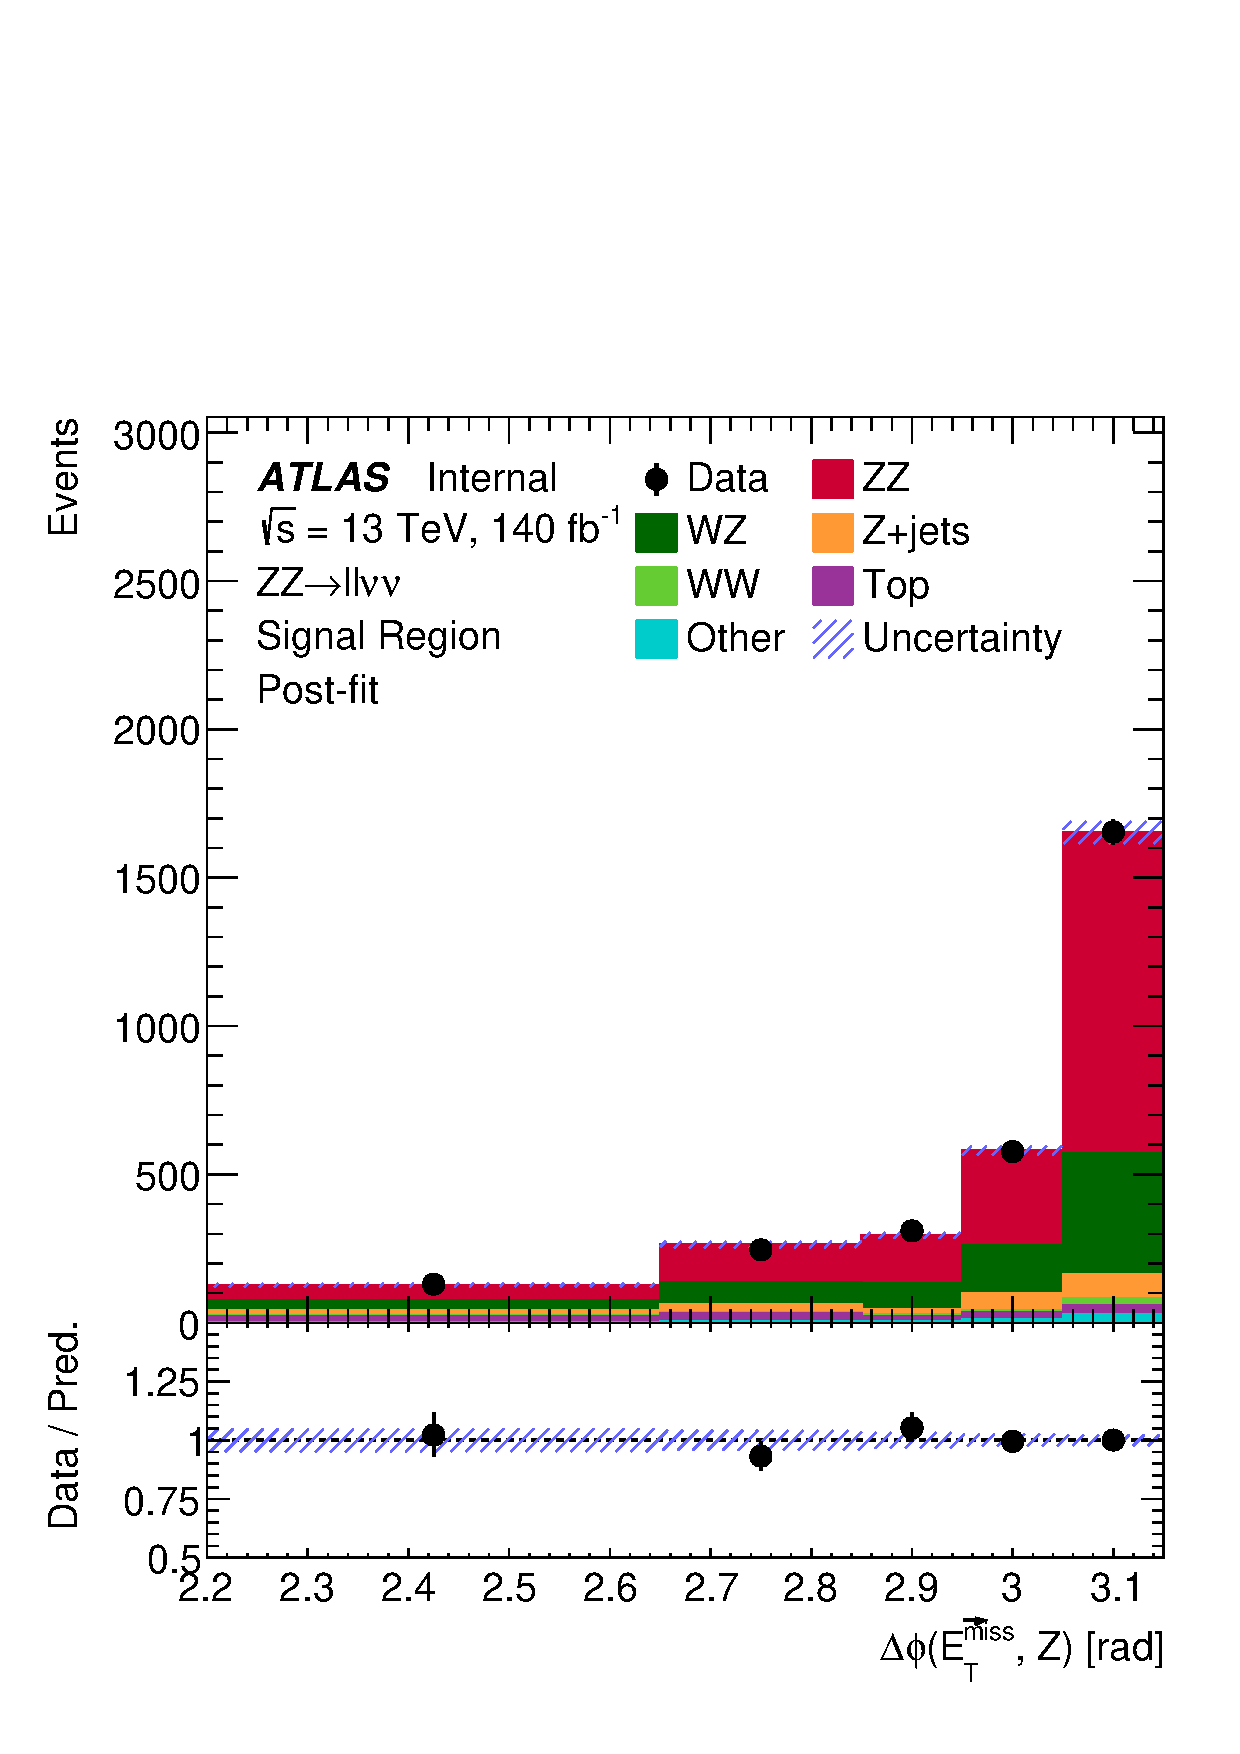
\includegraphics[width=0.32\linewidth]{figures/ch5-llvv/kin-distribution/SignalR_postFit-ZZ.pdf}
} 
    \subfloat[]{
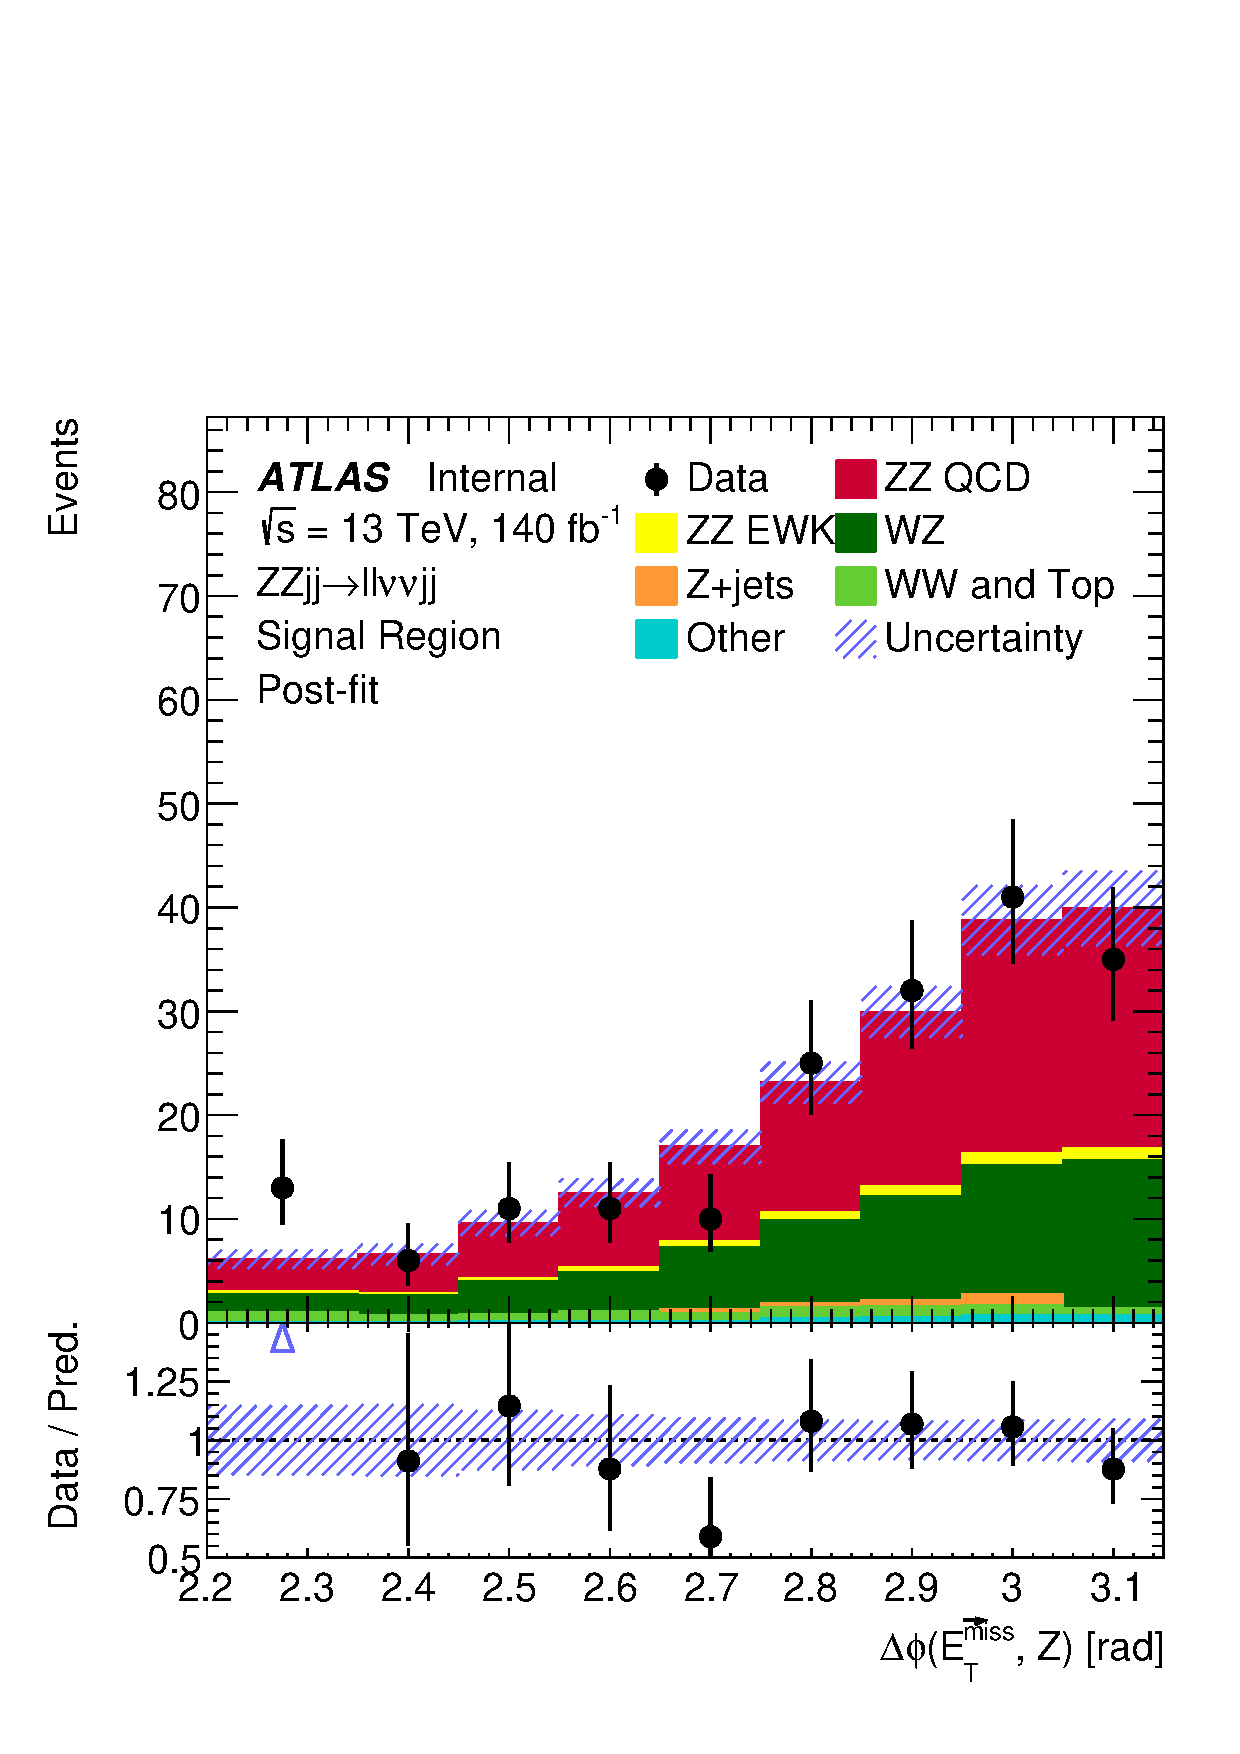
\includegraphics[width=0.32\linewidth]{figures/ch5-llvv/kin-distribution/SignalR_postFit-ZZjj.pdf}
}\\
    \subfloat[]{
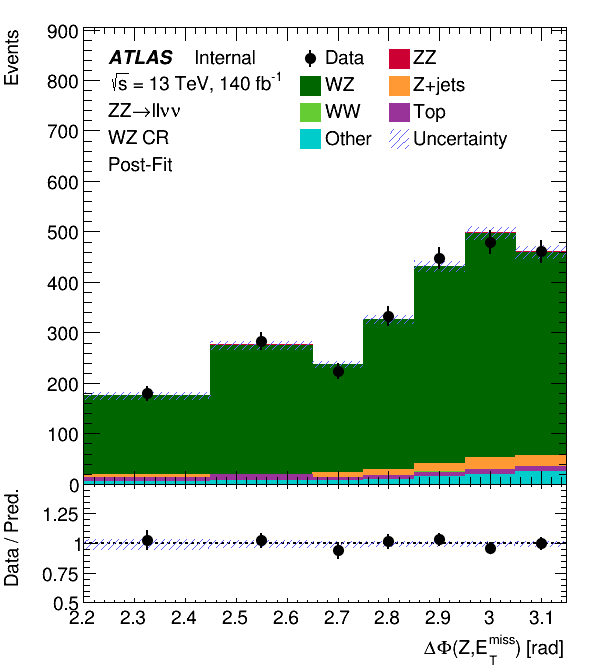
\includegraphics[width=0.325\linewidth]{figures/ch5-llvv/kin-distribution/WZ_postFit-ZZ.png}
}
    \subfloat[]{
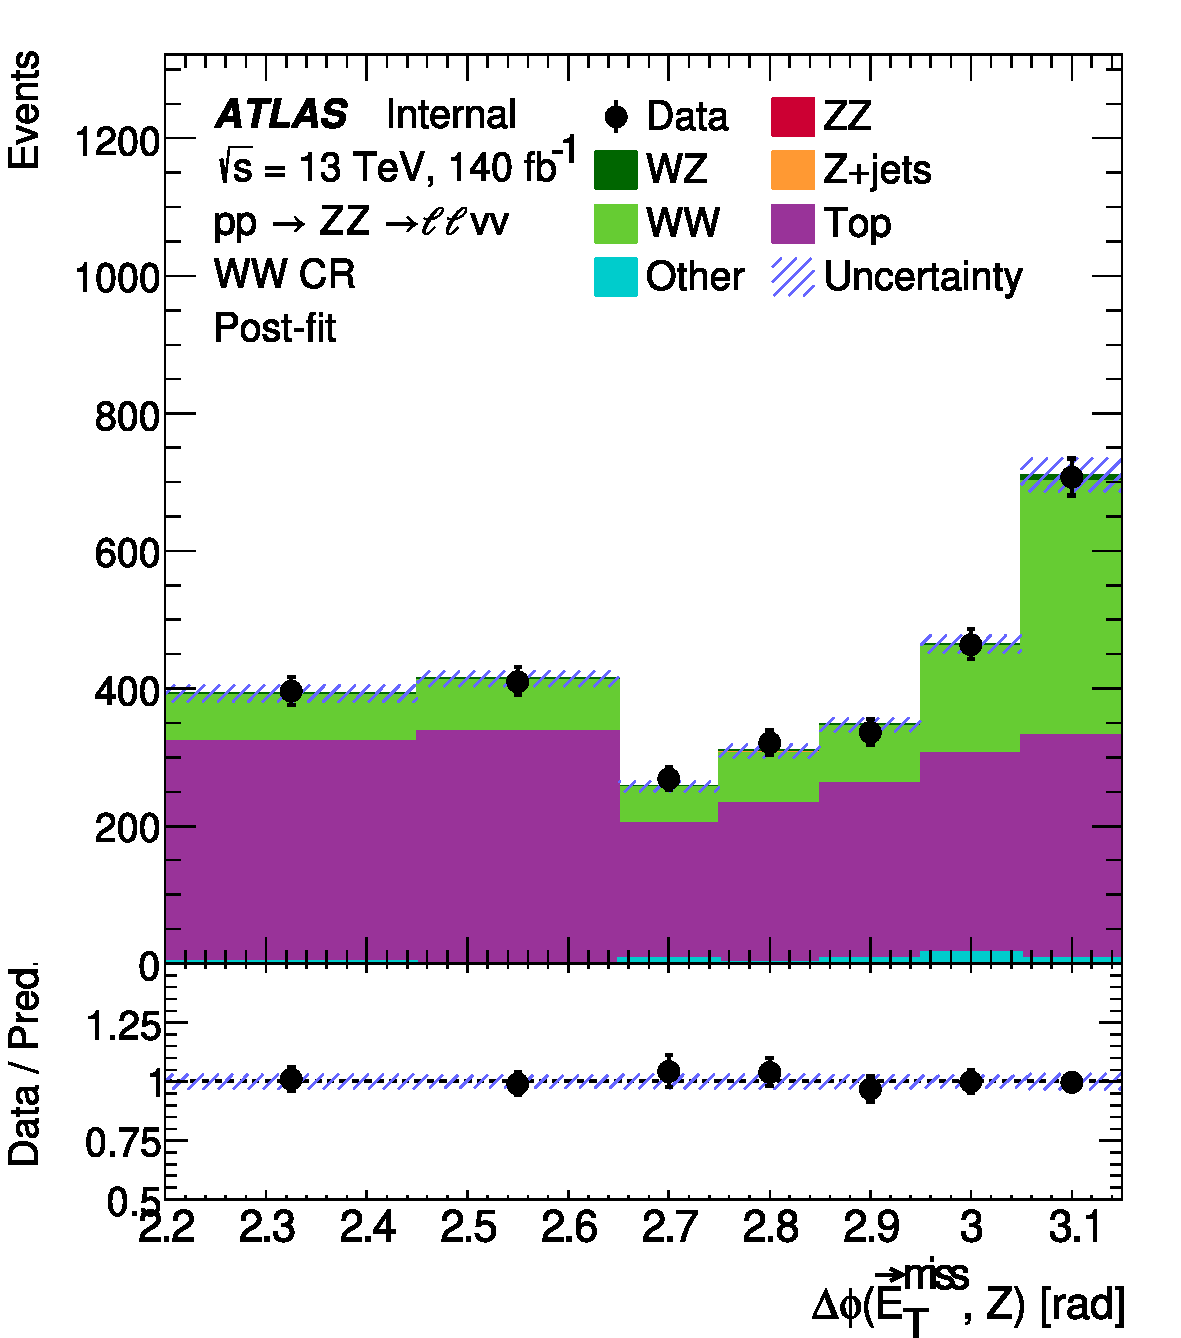
\includegraphics[width=0.32\linewidth]{figures/ch5-llvv/kin-distribution/EMU_A_postFit-ZZ.pdf}
}
    \subfloat[]{
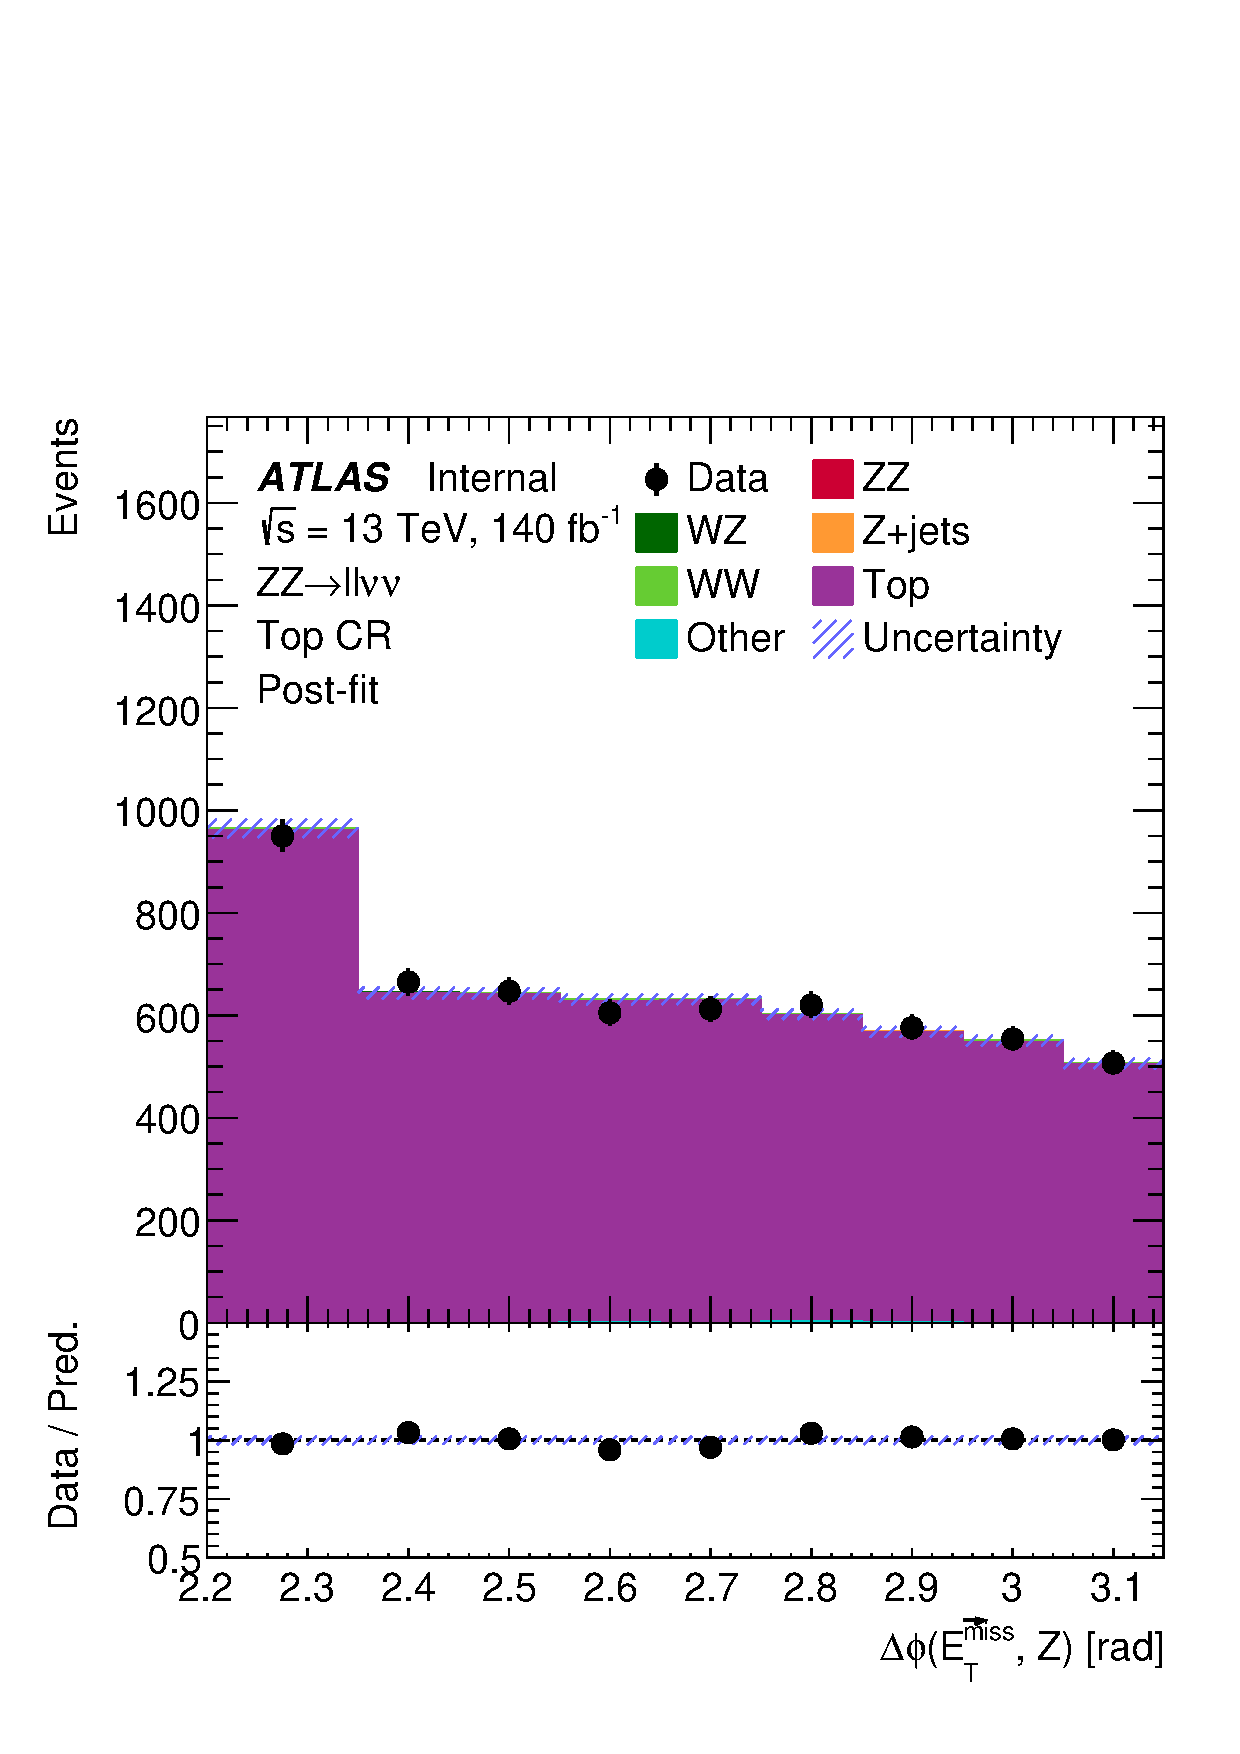
\includegraphics[width=0.32\linewidth]{figures/ch5-llvv/kin-distribution/EMU_B_postFit-ZZ.pdf}
}\\
    \subfloat[]{
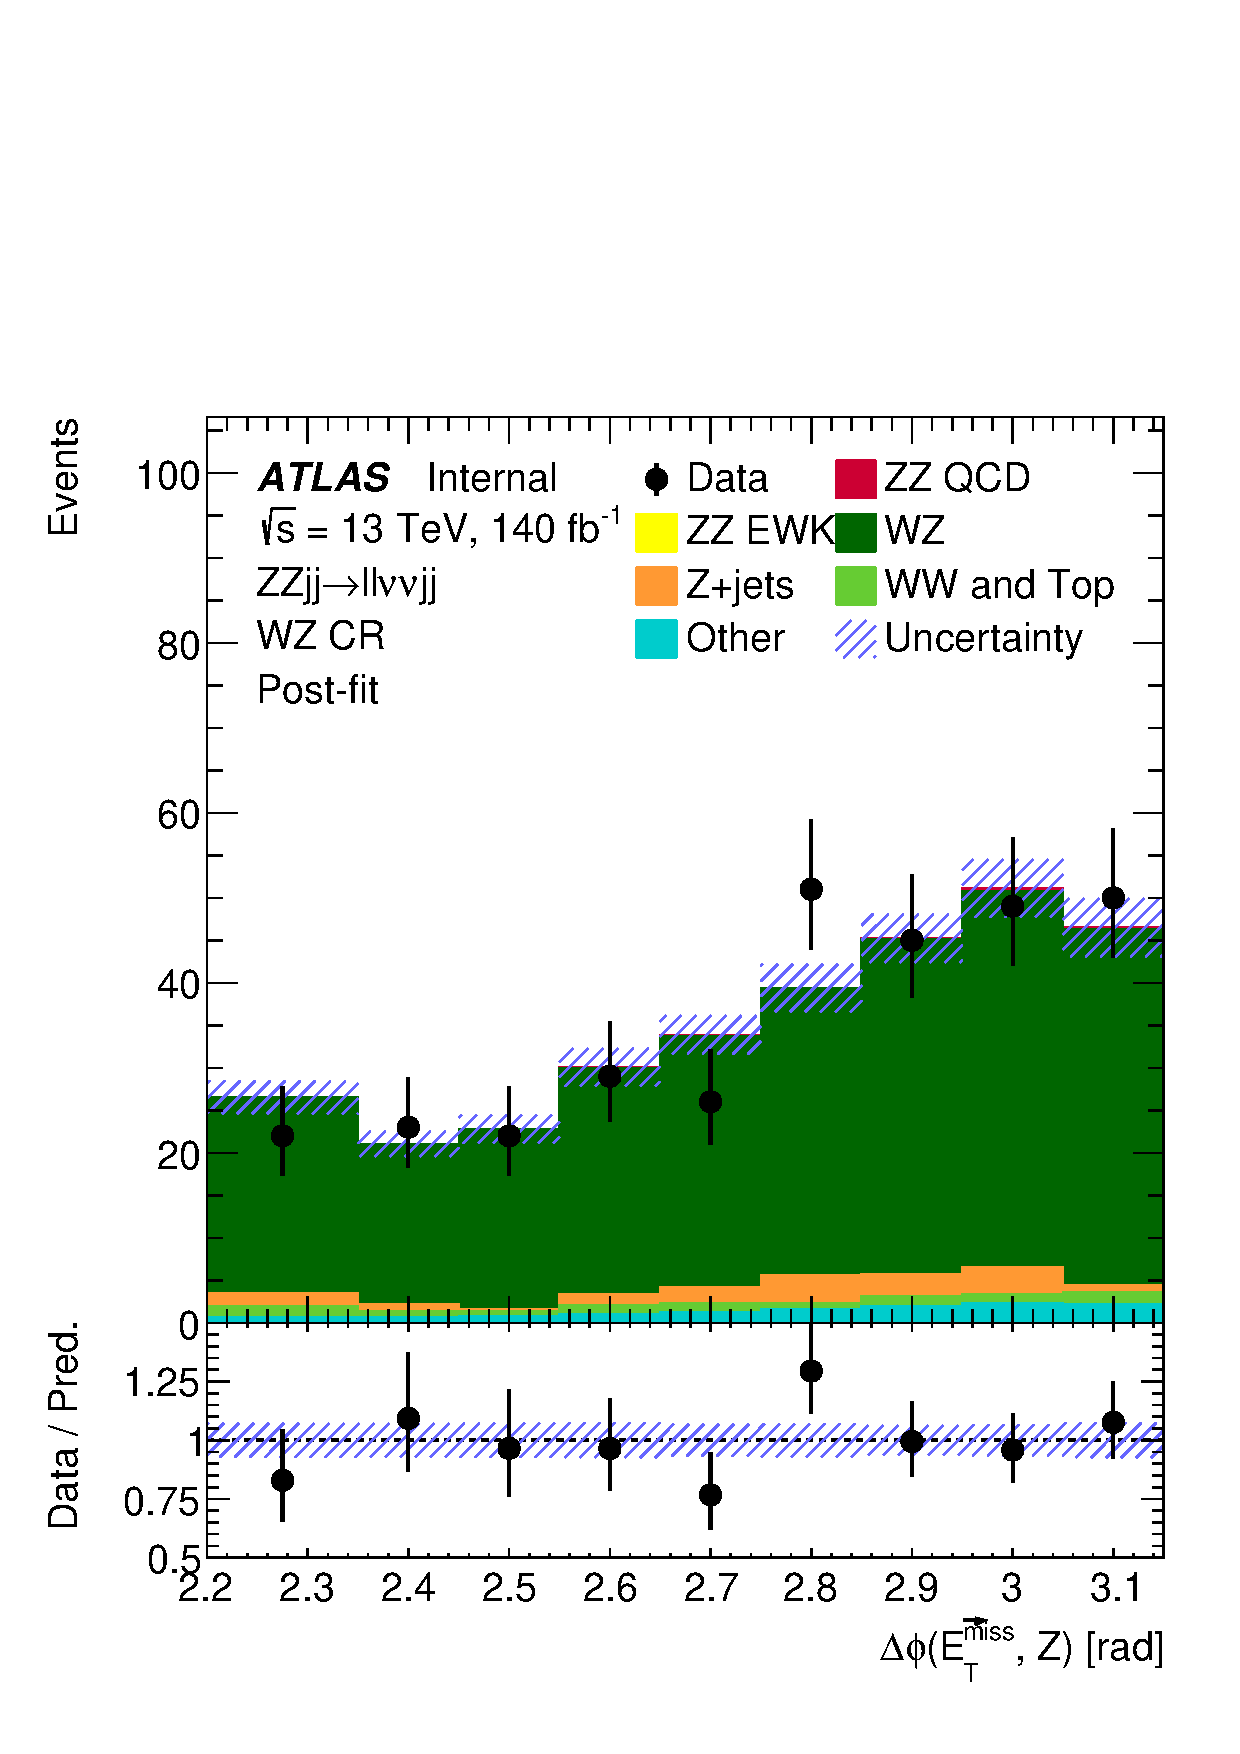
\includegraphics[width=0.325\linewidth]{figures/ch5-llvv/kin-distribution/WZ_postFit-ZZjj.pdf}
}
    \subfloat[]{
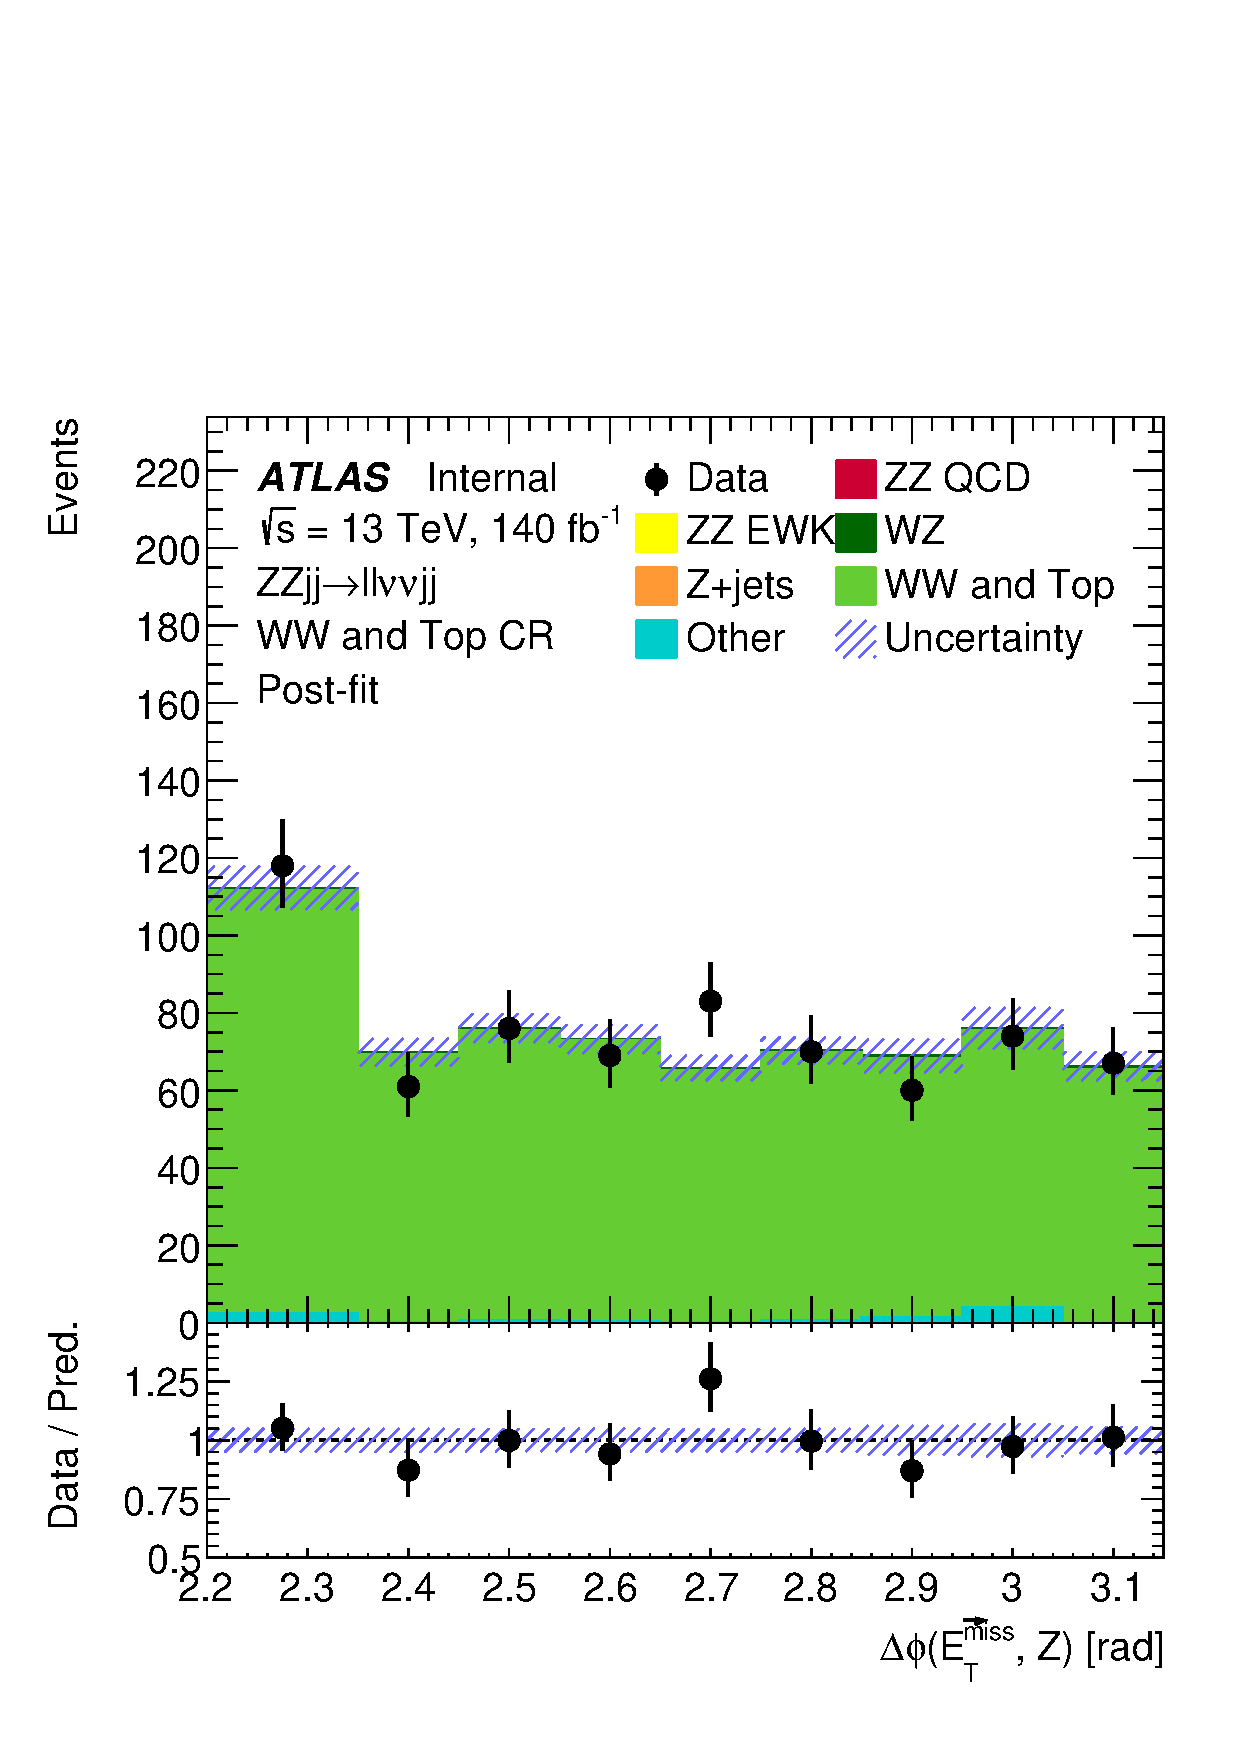
\includegraphics[width=0.325\linewidth]{figures/ch5-llvv/kin-distribution/EMU_postFit-ZZjj.pdf}
}
    \subfloat[]{
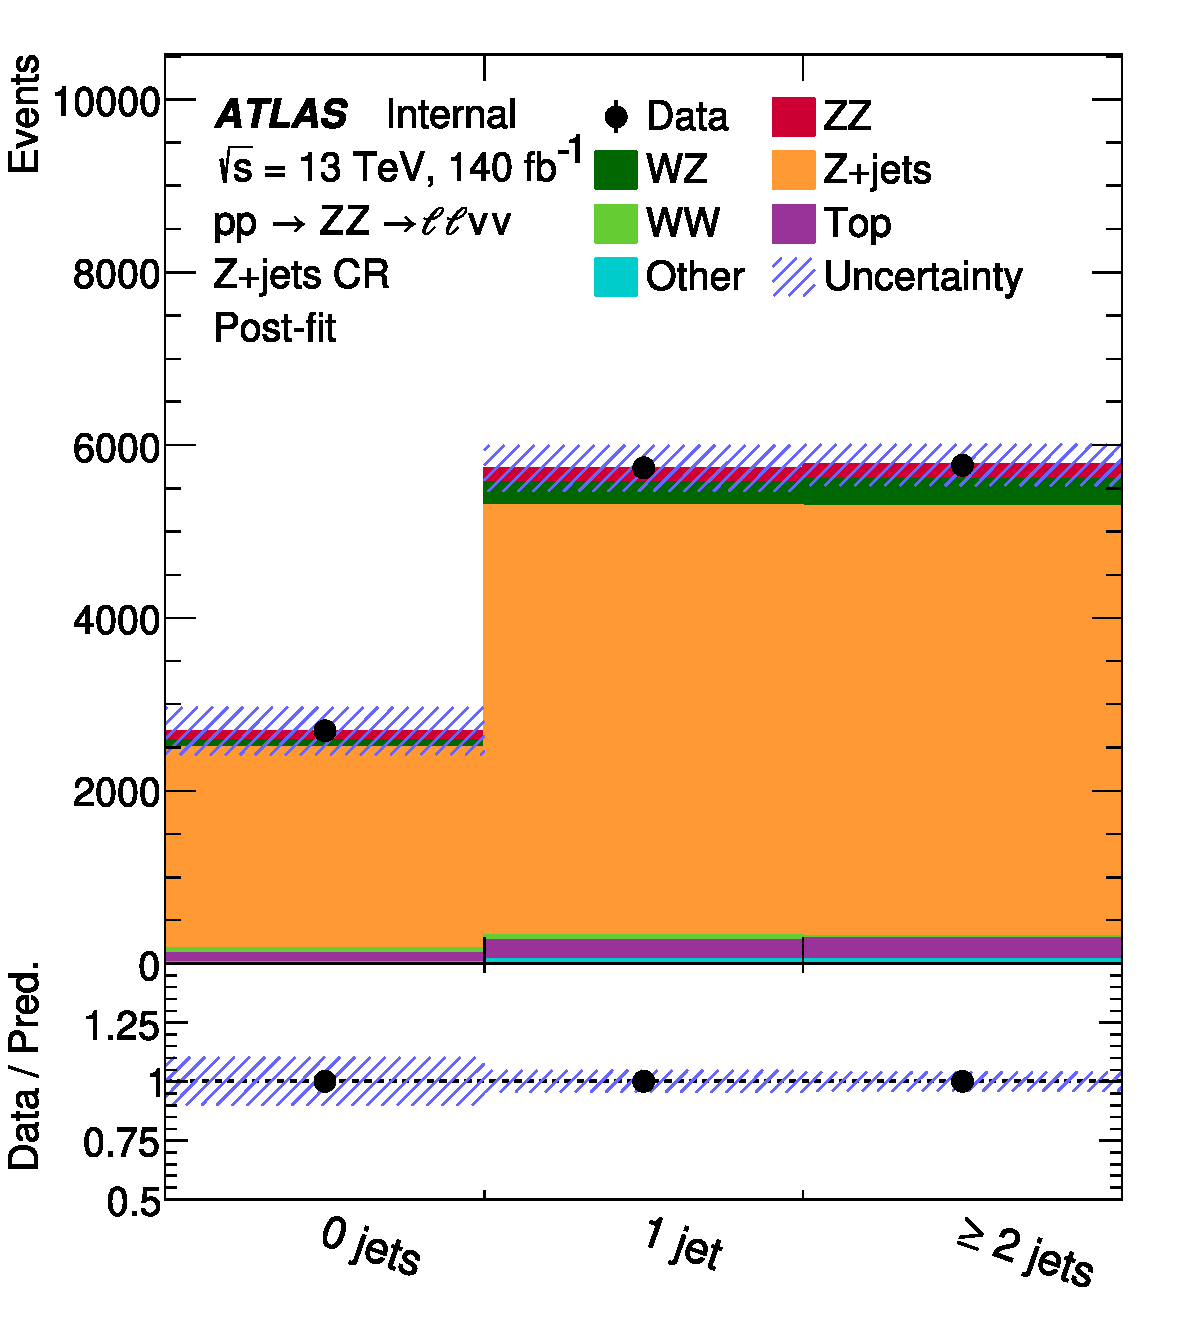
\includegraphics[width=0.325\linewidth]{figures/ch5-llvv/kin-distribution/Zj_VR_nJ_postFit-ZZ.pdf}
}
  \caption{The post-fit distributions of $\Delta\phi(\vec{E}_{\text{T}}^{\text{miss}}, \text{Z})$. Panels (a) and (b) show the signal regions for the inclusive $\text{ZZ}$ and $\text{ZZ}jj$ production, respectively. The ``Other'' category counts events from processes of $\text{ZZ} \to 4\ell, 2\ell 2q$, $\text{VVV}~(\text{V}=\text{W,Z})$, $\text{W}j$, $\text{Z} \to \tau\tau$, and $\text{WH}$. Figures (c), (d), and (e) illustrate the background CRs for inclusive $\text{ZZ}$ production, while panels (f) and (g) display the $\text{ZZ}jj$ CRs. Figure (h) presents the post-fit event yields for background events in the $\text{Z}$+0, 1, and $\ge 2$ jets CRs for the inclusive $\text{ZZ}$ analysis. Data points are shown with statistical error bars, while the shaded band represents the total post-fit uncertainty on the prediction, with combined statistical and systematic uncertainties.}
  \label{fig:postfit_observed_ZZCR}
\endminipage\hfill
\end{figure}

Additional post-fit kinematic distributions for the inclusive $\text{ZZ}$ SR are shown in the top row of Figure~\ref{fig:postfit_observed}: 
(a) the transverse momentum of the leading lepton, $p_{\text{T}}^{\text{leading-lepton}}$, 
(b) the missing transverse energy, $E_{\text{T}}^{\text{miss}}$, and 
(c) the azimuthal angle separation between the two charged leptons, $\Delta\phi(\ell, \ell)$. 
For the $\text{ZZ}jj$ SR, the bottom row shows: 
(d) the transverse momentum of the leading jet, $p_{\text{T}}^{\text{leading-jet}}$, 
(e) the invariant mass of the dijet system, $m_{jj}$, and 
(f) the transverse mass of the $\text{ZZ}$ system, $m_{\text{T}}^{\text{ZZ}}$. 

The data points are shown with statistical uncertainties, while the shaded band represents the total post-fit uncertainty in the prediction, including both statistical and systematic components. 
Overall, good agreement between data and MC predictions is observed across all distributions.


\begin{figure}[!htbp]
\minipage{1\textwidth}
\centering
   \subfloat[]{
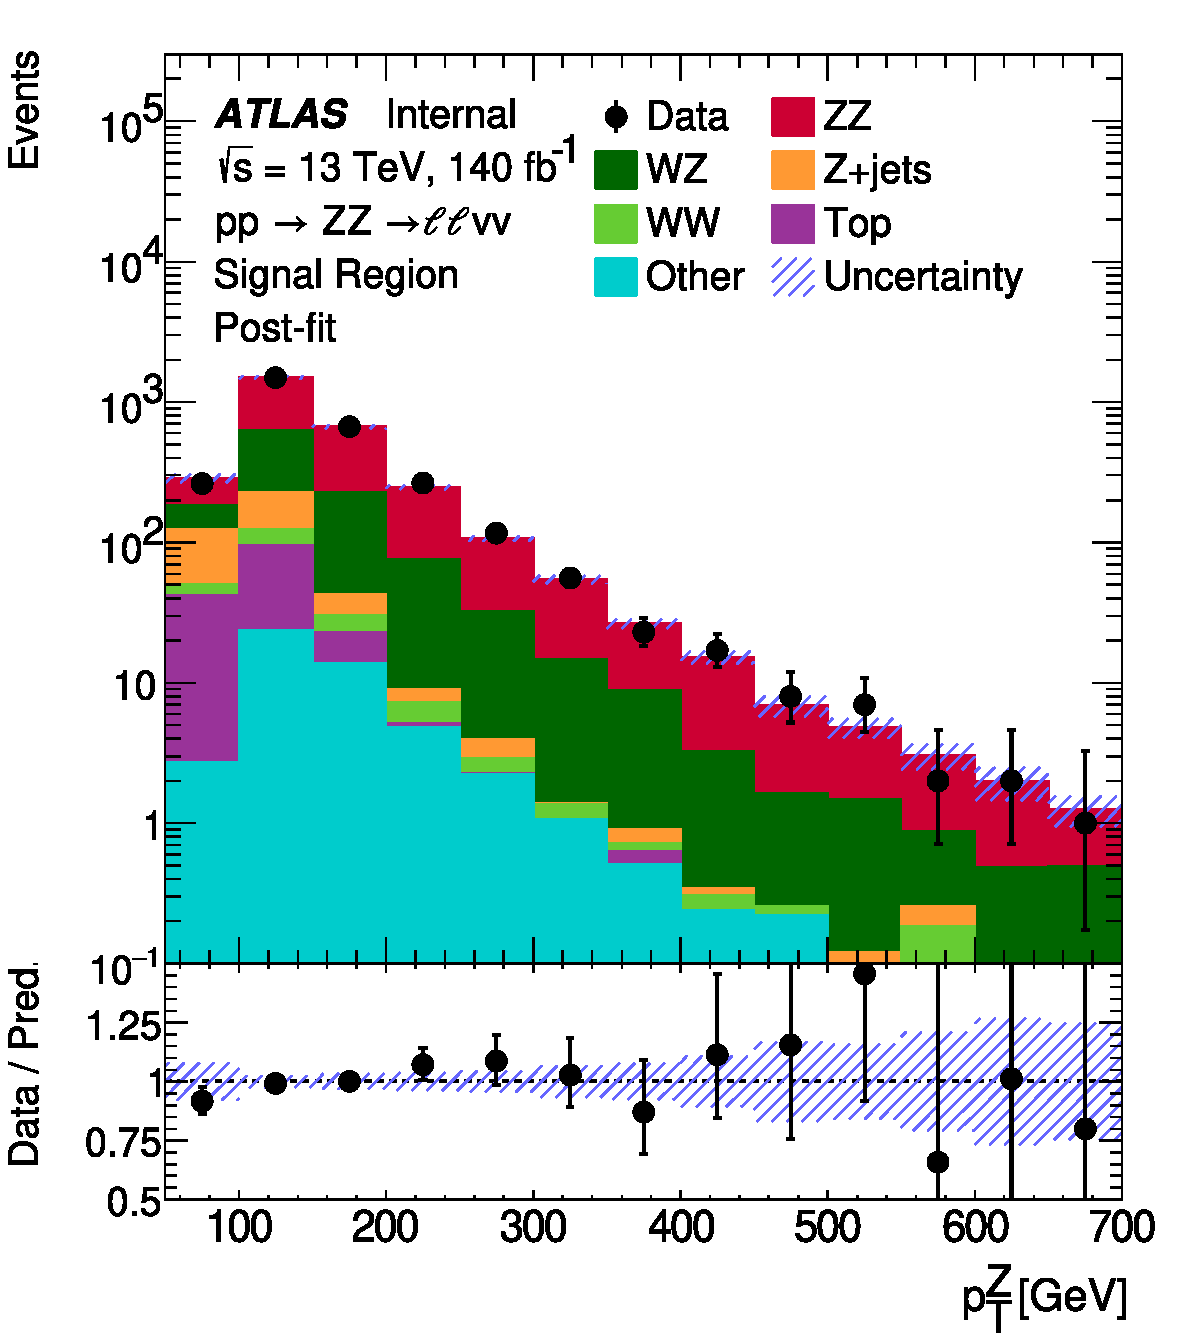
\includegraphics[width=0.32\linewidth]{figures/ch5-llvv/kin-distribution/Val_green_ptZ50_postFit-ZZ.pdf}
}
    \subfloat[]{
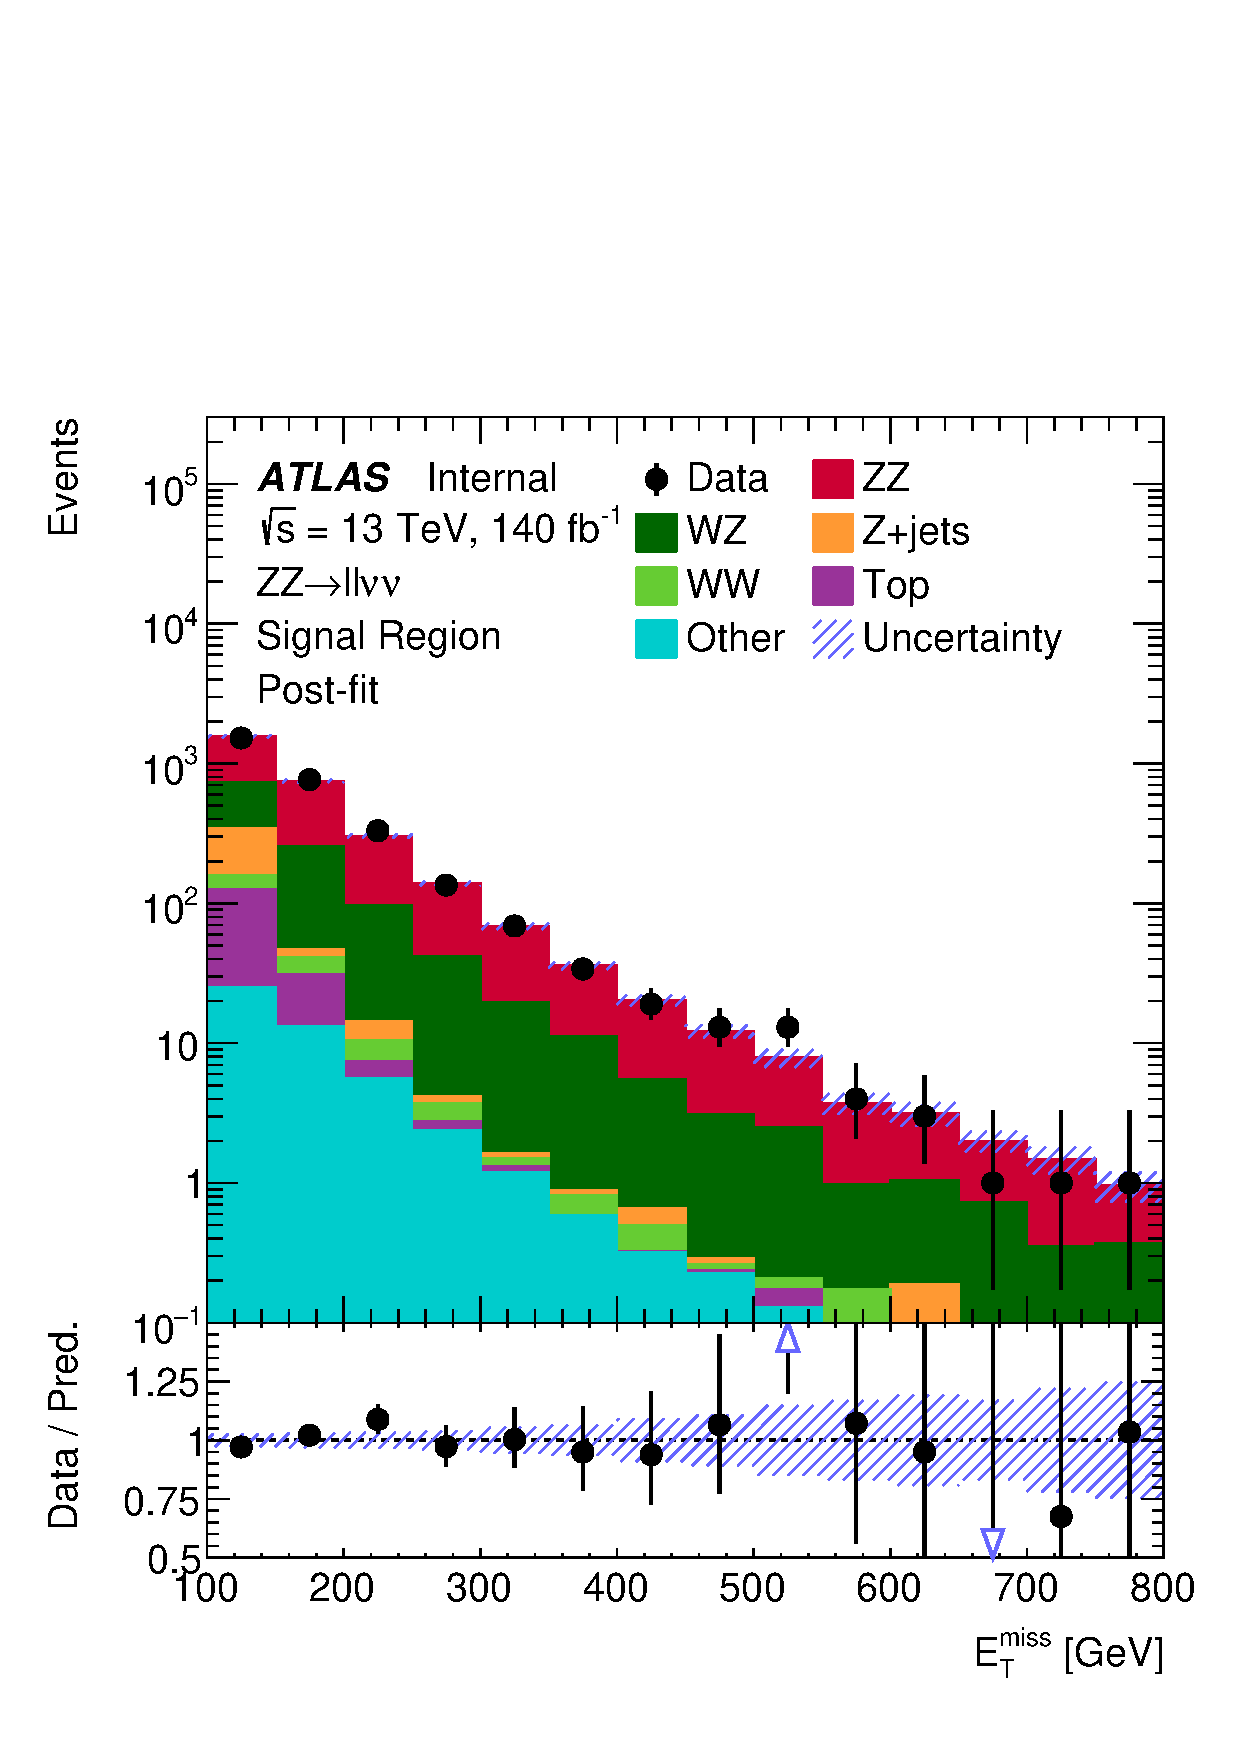
\includegraphics[width=0.32\linewidth]{figures/ch5-llvv/kin-distribution/Val_green_met50_postFit-ZZ.pdf}
}
    \subfloat[]{
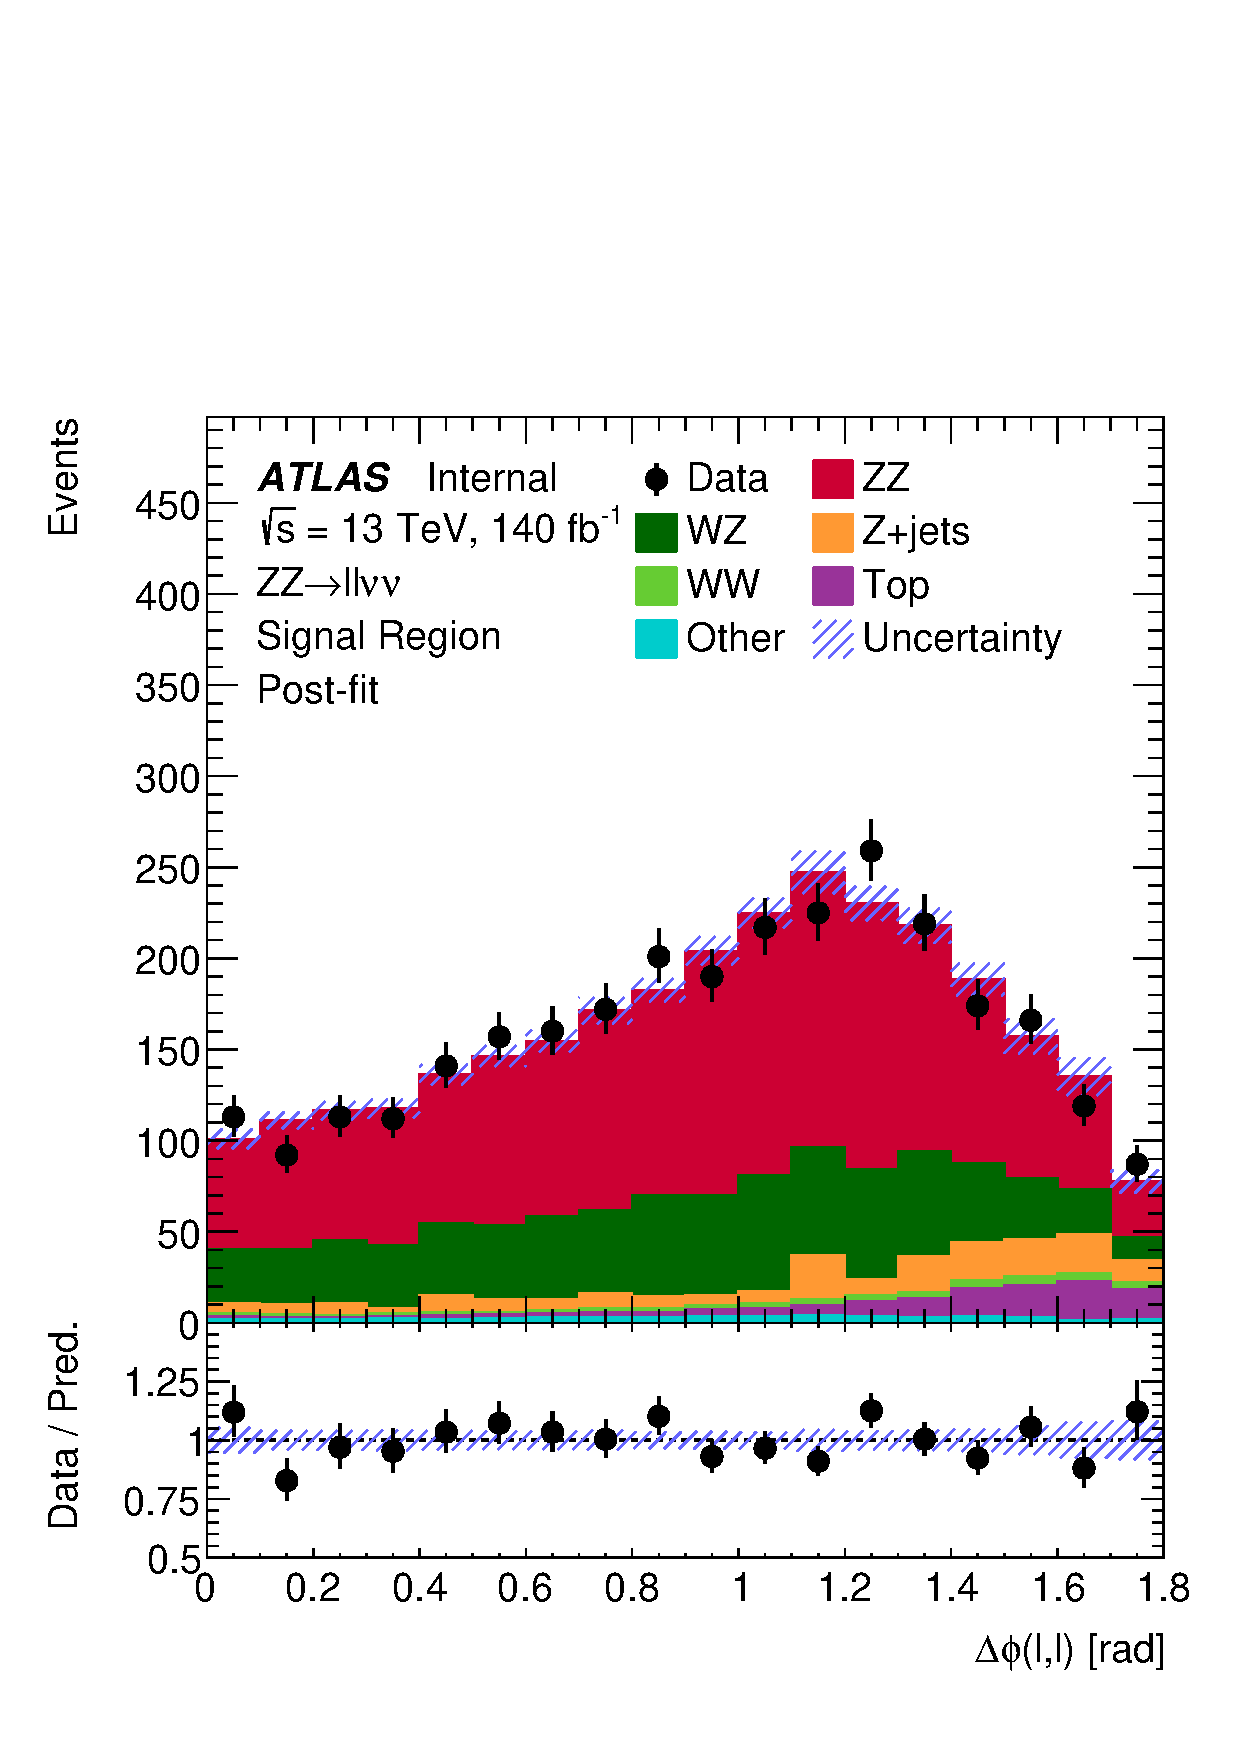
\includegraphics[width=0.32\linewidth]{figures/ch5-llvv/kin-distribution/Val_green_dPhill50_postFit-ZZ.pdf}
}\\
    \subfloat[]{
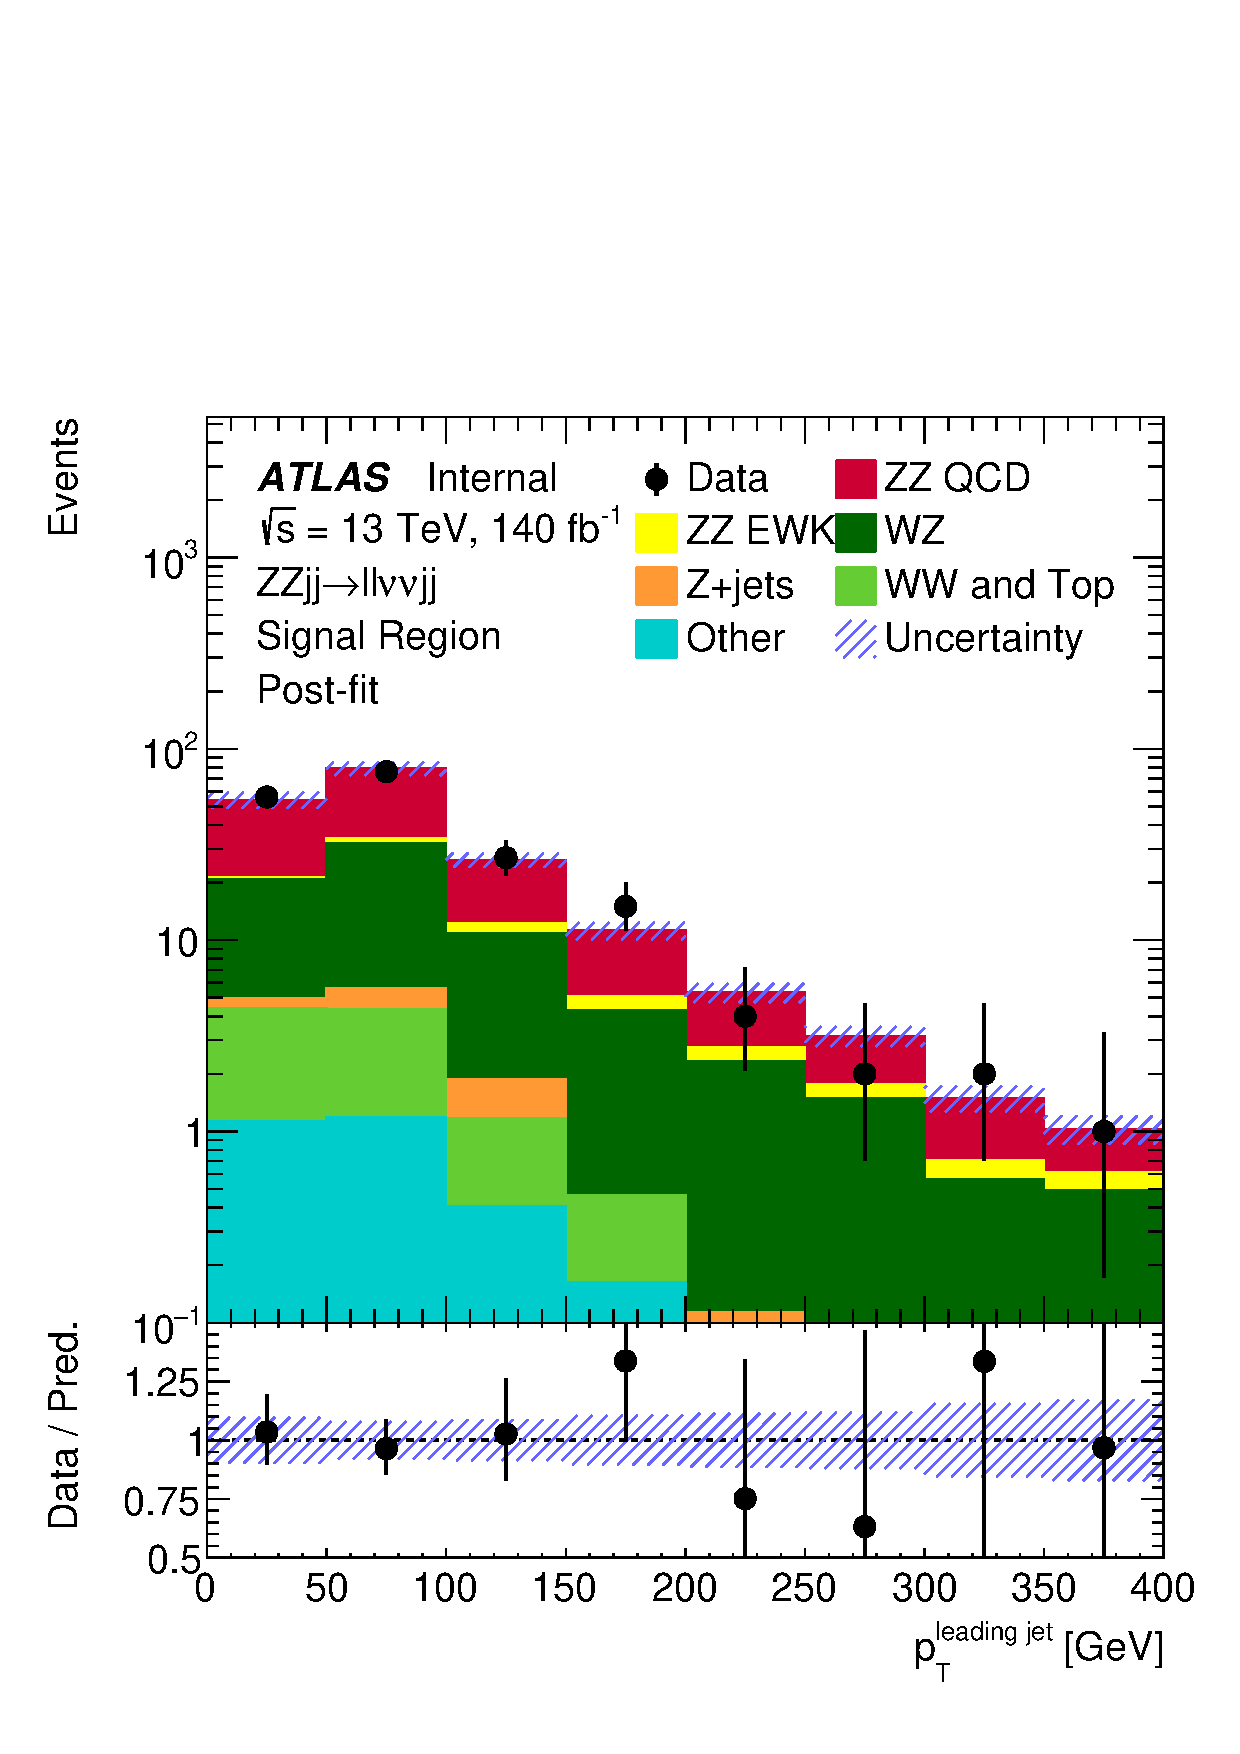
\includegraphics[width=0.32\linewidth]{figures/ch5-llvv/kin-distribution/SignalR_Jpt50_postFit-ZZjj.pdf}
}
    \subfloat[]{
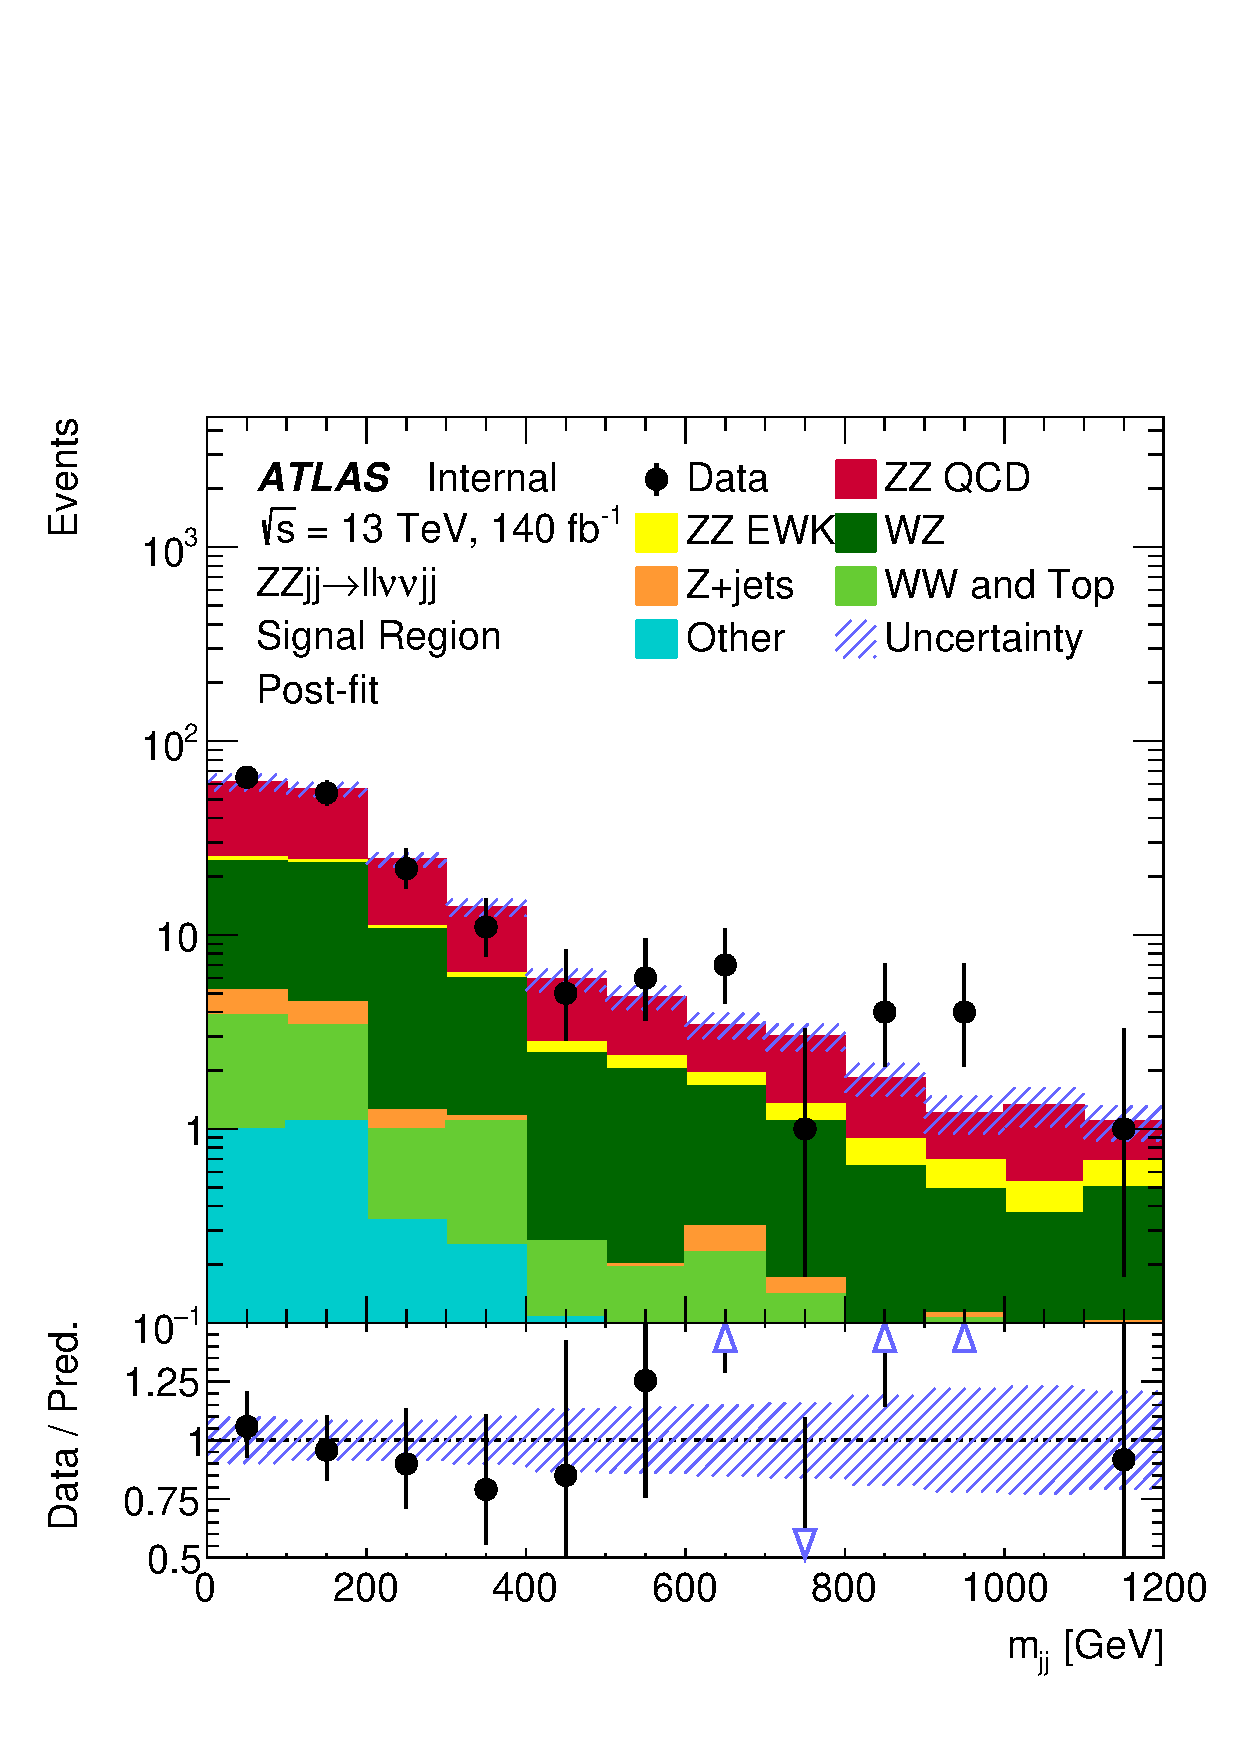
\includegraphics[width=0.32\linewidth]{figures/ch5-llvv/kin-distribution/SignalR_mjj100_postFit-ZZjj.pdf}
}
    \subfloat[]{
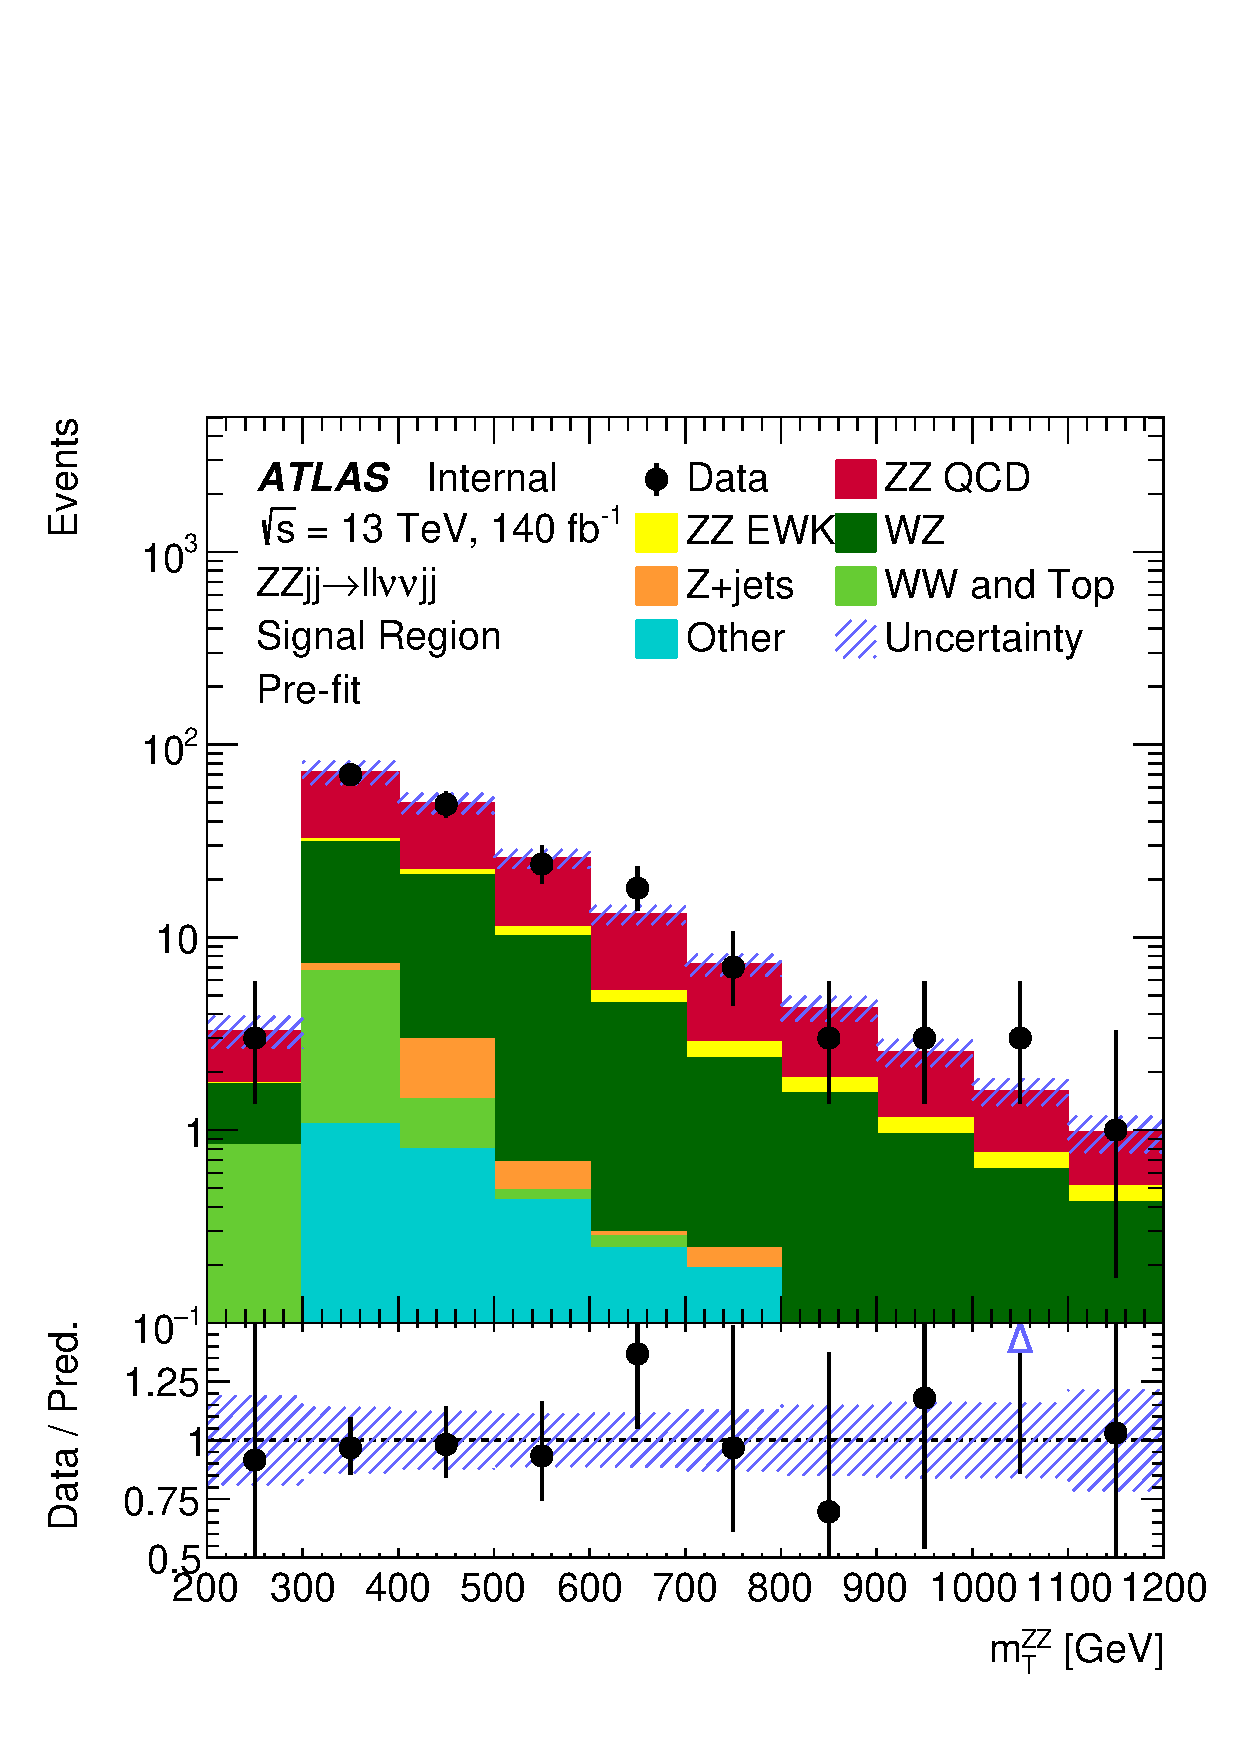
\includegraphics[width=0.32\linewidth]{figures/ch5-llvv/kin-distribution/SignalR_mtzz100_log-ZZjj.pdf}
}
  %\caption{Post-fit kinematic distributions for the inclusive $ZZ$ SR are shown in the top row: (a) the transverse momentum of the leading lepton $p_\text{T}^\text{leading-lepton}$, (b) the missing transverse energy $E_\text{T}^\text{miss}$ and (c) the azimuthal angle separation between two charged leptons $\Delta\phi(\ell, \ell)$. For the $ZZjj$ SR, the bottom row shows: (d) the leading jet $p_\text{T}^\text{leading-jet}$, (e) the invariant mass of the dijet system $m_\text{jj}$, 
  \caption{Post-fit kinematic distributions for the inclusive $\text{ZZ}$ SR are shown in the top row: (a) the transverse momentum of the lepton pair, (b) the missing transverse energy $E_{\text{T}}^{\text{miss}}$, and (c) the azimuthal angle separation between two charged leptons $\Delta\phi(\ell, \ell)$. For the $\text{ZZ}jj$ SR, the bottom row shows: (d) the leading jet $p_{\text{T}}^{\text{leading-jet}}$, (e) the invariant mass of the dijet system $m_{jj}$, 
  and (f) the transverse mass of the $\text{ZZ}$ system $m_{\text{T}}^{\text{ZZ}}$. The data points are shown with statistical error bars, while the shaded band represents the total post-fit uncertainty in the prediction, with combined statistical and systematic uncertainties.}
  \label{fig:postfit_observed}
\endminipage\hfill
\end{figure}


The fiducial cross-sections for the processes $\text{ZZ} \to \ell\ell\nu\nu$ and $\text{ZZ}jj \to \ell\ell\nu\nu jj$ in their respective fiducial phase spaces are calculated by multiplying the measured signal strengths ($\mu_{\text{S}}^{\text{ZZ}}$ and $\mu_{\text{S}}^{\text{ZZ}jj}$) by the SM cross-section predictions as shown in Table~\ref{tab:sherpa-xs}.

The measured fiducial cross-section for the inclusive $\text{ZZ} \to \ell\ell\nu\nu$ production process is found to be
\begin{equation*}
\sigma_{\text{ZZ}}^{\text{fid}} = 21.03 \pm 0.73_{\text{stat}} \pm 0.57_{\text{exp}} \pm 0.18_{\text{theory}} \pm 0.18_{\text{lumi}}~\text{fb},
\end{equation*} 
where the uncertainty is separated into the data statistical uncertainty (stat), the uncertainty from experimental systematic uncertainties (exp), the uncertainty from theory systematic uncertainties (theory), and the luminosity uncertainty (lumi). 
The measured cross-section is in agreement with the SM prediction of $20.1 \pm 1.1~\text{fb}$ from \textsc{Sherpa}+\textsc{MadGraph5} and $21.03 \pm 0.30~\text{fb}$ from \textsc{Matrix}. 

For the $\text{ZZ}jj \to \ell\ell\nu\nu jj$ production process, the measured fiducial cross-section is 
\begin{equation*}
\sigma_{\text{ZZ}jj}^{\text{fid}} = 0.96^{+0.15}_{-0.11\text{ (stat)}} \pm 0.10_{\text{exp}} \pm 0.04_{\text{theory}} \pm 0.01_{\text{lumi}}~\text{fb}.
\end{equation*}
This is compatible with the theoretical prediction of $0.94 \pm 0.20~\text{fb}$ from \textsc{Sherpa}+\textsc{MadGraph5}. 

The $\text{ZZ} \to \ell\ell\nu\nu$ fiducial production cross-section is extrapolated to the total phase space, using the fiducial acceptance reported in Table~\ref{tab:zz-xs} and the branching ratio~\cite{Zyla:2020zbs} of the $\text{ZZ}$ decay mode $\text{ZZ} \to 2\ell 2\nu$. 

The total $pp \to \text{ZZ}$ production is found to be:
\begin{equation*}
\sigma^{\text{total}}_{\text{measured}}(pp \to \text{ZZ}) = 15.38 \pm 0.81~\text{pb}.
\end{equation*}
This measurement is in agreement with the SM prediction calculated using \textsc{Matrix}: $\sigma^{\text{total}}_{\text{SM}}(pp \to \text{ZZ}) = 15.40 \pm 0.38~\text{pb}$.


  %include text of cross-section measurement
\input{chapters/Ch5-ZZxs/5_5_unfolding}
\subsection{Measured Differential Cross-sections}
\label{diff-xs}

Differential cross-sections are measured in the fiducial phase spaces by counting data events in each bin of the relevant observables, subtracting the expected background contributions, and correcting for detector effects. Detector-level distributions are unfolded to stable-particle level using an iterative Bayesian method~\cite{DAgostini1995}, which accounts for resolution effects, reconstruction inefficiencies, and bin migrations. Response matrices derived from simulated signal samples encode the probability of an event generated in a given particle-level bin being reconstructed in a corresponding detector-level bin. 

The number of iterations, typically between two and five depending on the observable, is optimised to balance statistical uncertainty and unfolding stability. The binning is defined using purity and efficiency criteria to ensure reliable unfolding and preserve the distribution shapes. The final bin of each observable is open-ended and extends to the kinematic limit, with no separate overflow bin. Validation studies using nominal and alternative samples show no significant bias. 
The kinematic variables used for the differential cross-section measurements are summarised in Table~\ref{tab:diff-var}.
\begin{table}[!hbtp]
    \centering
    \scriptsize
    \renewcommand{\arraystretch}{1.5}
    \begin{tabular}{l c c}
    \hline
  \textbf{Observable description} &  \textbf{Observable} &  \textbf{SR} \\
     \hline 
      Azimuthal angular separation of the two leptons & $\Delta\phi(\ell, \ell)$  & $ZZ$ and $ZZjj$ \\
      Transverse momentum of the leading lepton  &  $p_\text{T}^{\text{leading lepton}}$ & $ZZ$ only \\  
      Transverse momentum of the Z boson  & $p_\text{T}^Z$ & $ZZ$ and $ZZjj$ \\  
      Rapidity of the visible $Z \rightarrow \ell\ell$  &    $|y^Z|$ & $ZZ$ and $ZZjj$ \\ 
      Transverse momentum of the $ZZ$ system  &  $p_\text{T}^{ZZ}$ & $ZZ$ and $ZZjj$ \\ 
       Transverse mass of the $ZZ$ system 
       &  $m_\text{T}^{ZZ}$ & $ZZ$ and $ZZjj$\\
     Number of jets                   &   $N_{jets}$ & $ZZ$ only\\  
 %   CP-sensitive angular variable (scenario 1)  & $sin(\phi_1)cos(\theta_1)$ & $ZZ$ only \\  \hline 
    CP-sensitive angular variable   &  $\sin(\varphi)\cos(\theta)$ & $ZZ$ only\\
    Invariant mass of the dijet system & $m_{jj}$ & $ZZjj$ only \\ 
    Transverse momentum of the leading jet & $p_\text{T}^{\text{leading jet}}$ & $ZZjj$ only \\ 
    \hline
    \end{tabular}
    \caption{\rm Kinematic variables for the differential cross-section measurements.} %through the unfolding procedure.}
    \label{tab:diff-var}
\end{table} 

A CP-sensitive angular variable, $\sin\varphi \cos\theta$, is constructed in the $ZZ$ signal region following Refs.~\cite{Chang:1994cs, STDM-2021-05, Semushin:2025uts}. The polar angle $\theta$ and azimuthal angle $\varphi$ are defined for the negatively charged lepton in the dilepton rest frame, with the $z$-axis aligned with the dilepton momentum in the $ZZ$ rest frame and the remaining axes forming a right-handed coordinate system. Since neutrinos from $Z\to\nu\bar{\nu}$ decays are not directly detected, the dineutrino momentum is approximated as $\vec{p}^{\,\nu\nu}=-\vec{p}^{\,\ell\ell}$, corresponding to the assumption that the $ZZ$ system is at rest in the laboratory frame. The differential cross-section for this observable is unfolded to particle level in the fiducial phase space.

Figures~\ref{fig:diff-xs-ZZ} and~\ref{fig:diff-xs-ZZjj} present the measured differential cross-sections. The quoted uncertainties include both statistical and systematic contributions propagated through the unfolding procedure. Statistical uncertainties dominate most bins, while systematic uncertainties become significant in specific kinematic regions.

The measured differential cross-sections in the $ZZ$ fiducial phase space show good agreement with SM predictions from the nominal \textsc{Sherpa}+\textsc{MadGraph5} simulation (denoted as \textsc{Sherpa+MG5}) and from the \textsc{Matrix} calculation. The \textsc{Matrix} predictions show slightly improved agreement with the data, consistent with the inclusion of NNLO QCD corrections.

In the $ZZjj$ fiducial phase space, the results are compared with SM predictions obtained using \textsc{Sherpa} for strong production and \textsc{MadGraph5} for electroweak production. The total uncertainties in the $ZZjj$ measurements are larger than those in the inclusive $ZZ$ phase space due to reduced event statistics and additional jet-related uncertainties. The \textsc{Sherpa} prediction describes the data well within uncertainties.


%%% differential cross-section Plots
\begin{figure}[!hbtp]
    \centering
    \subfloat[]{
    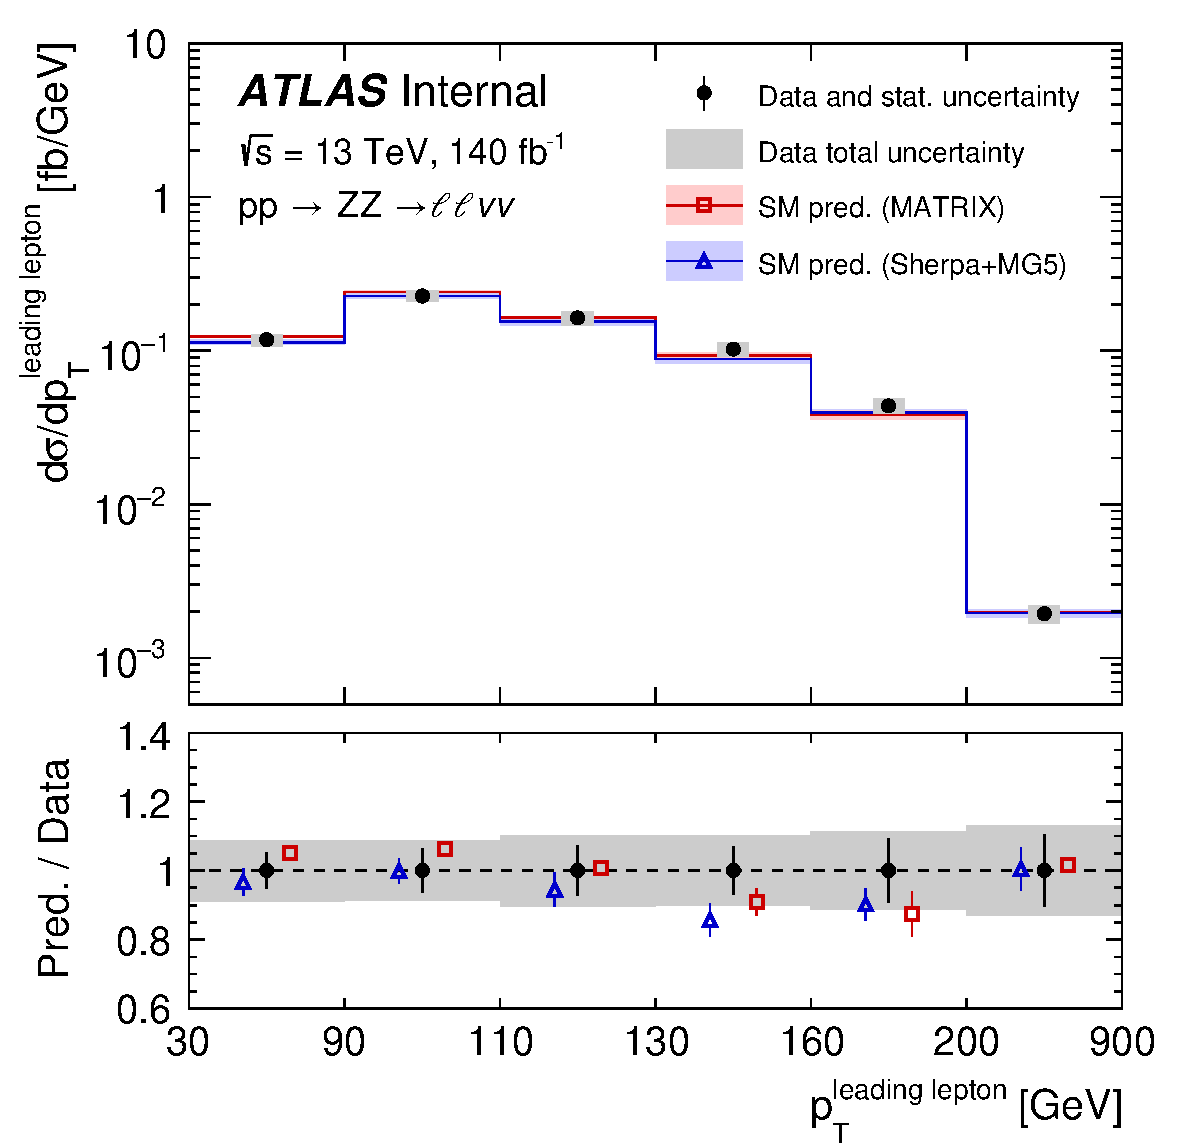
\includegraphics[width=0.32\linewidth]{figures/ch5-llvv/diff-xs/ZZ-pT_l1.pdf}
    }
    \subfloat[]{
    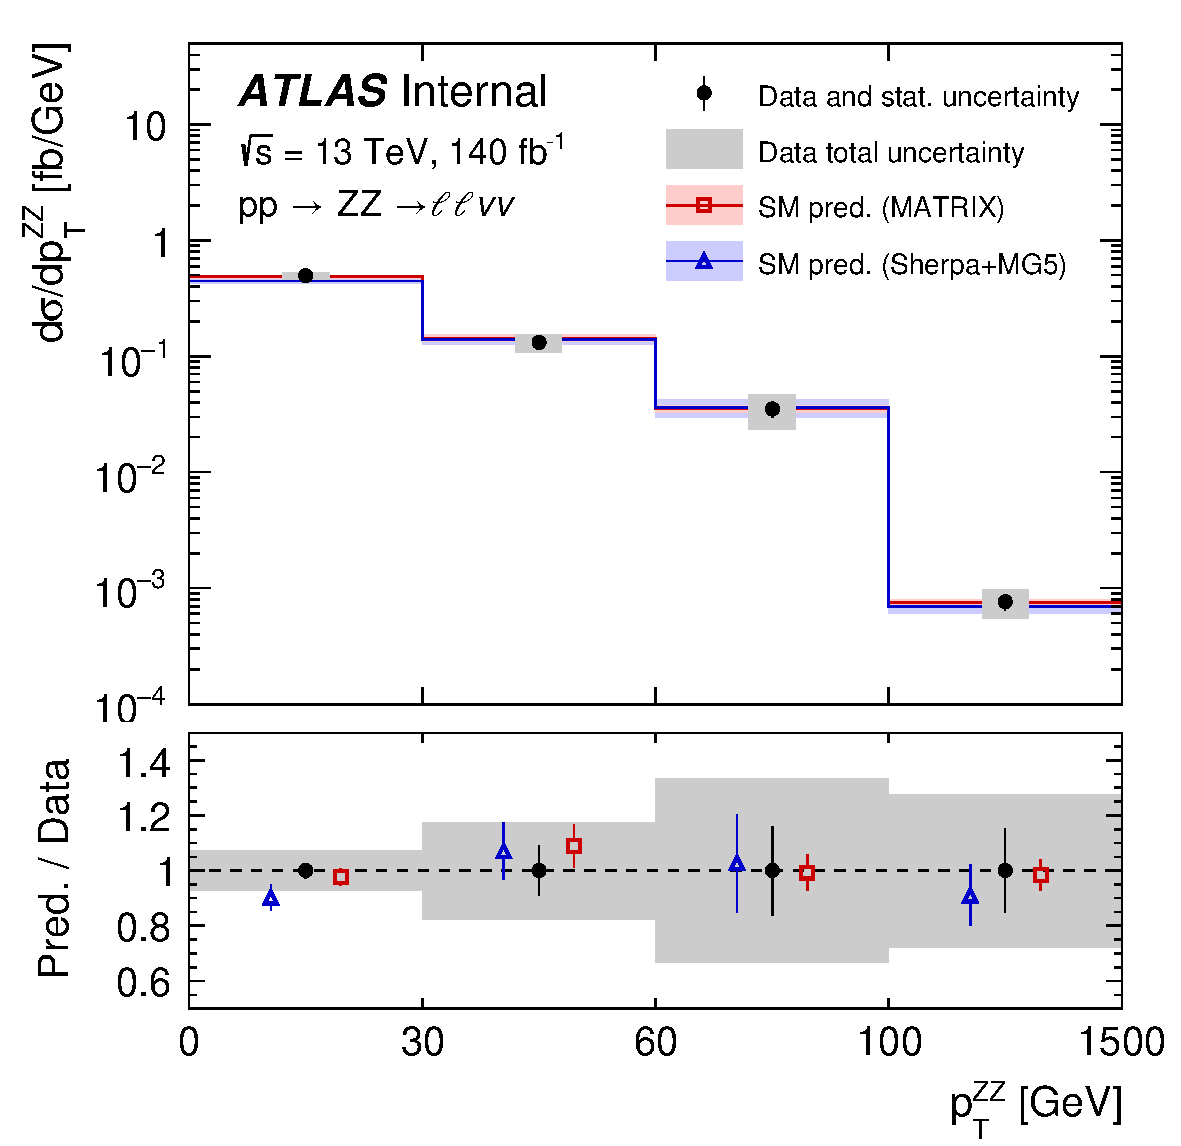
\includegraphics[width=0.32\linewidth]{figures/ch5-llvv/diff-xs/ZZ-pT_ZZ.pdf}
    }
    \subfloat[]{    
    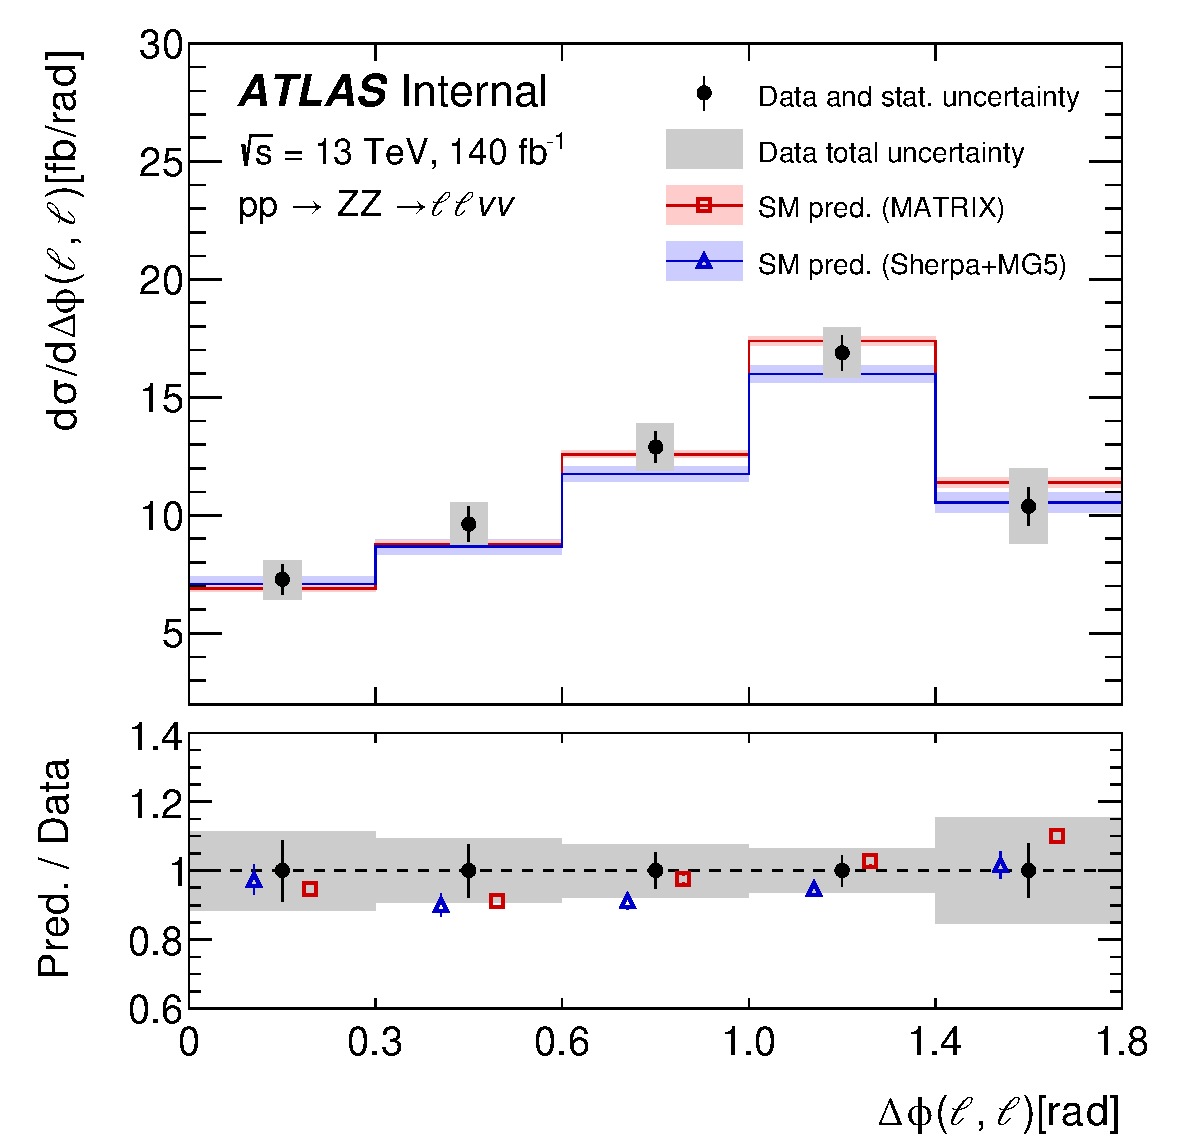
\includegraphics[width=0.32\linewidth]{figures/ch5-llvv/diff-xs/ZZ-dphi_ll.pdf}
    }\\
    \subfloat[]{    
    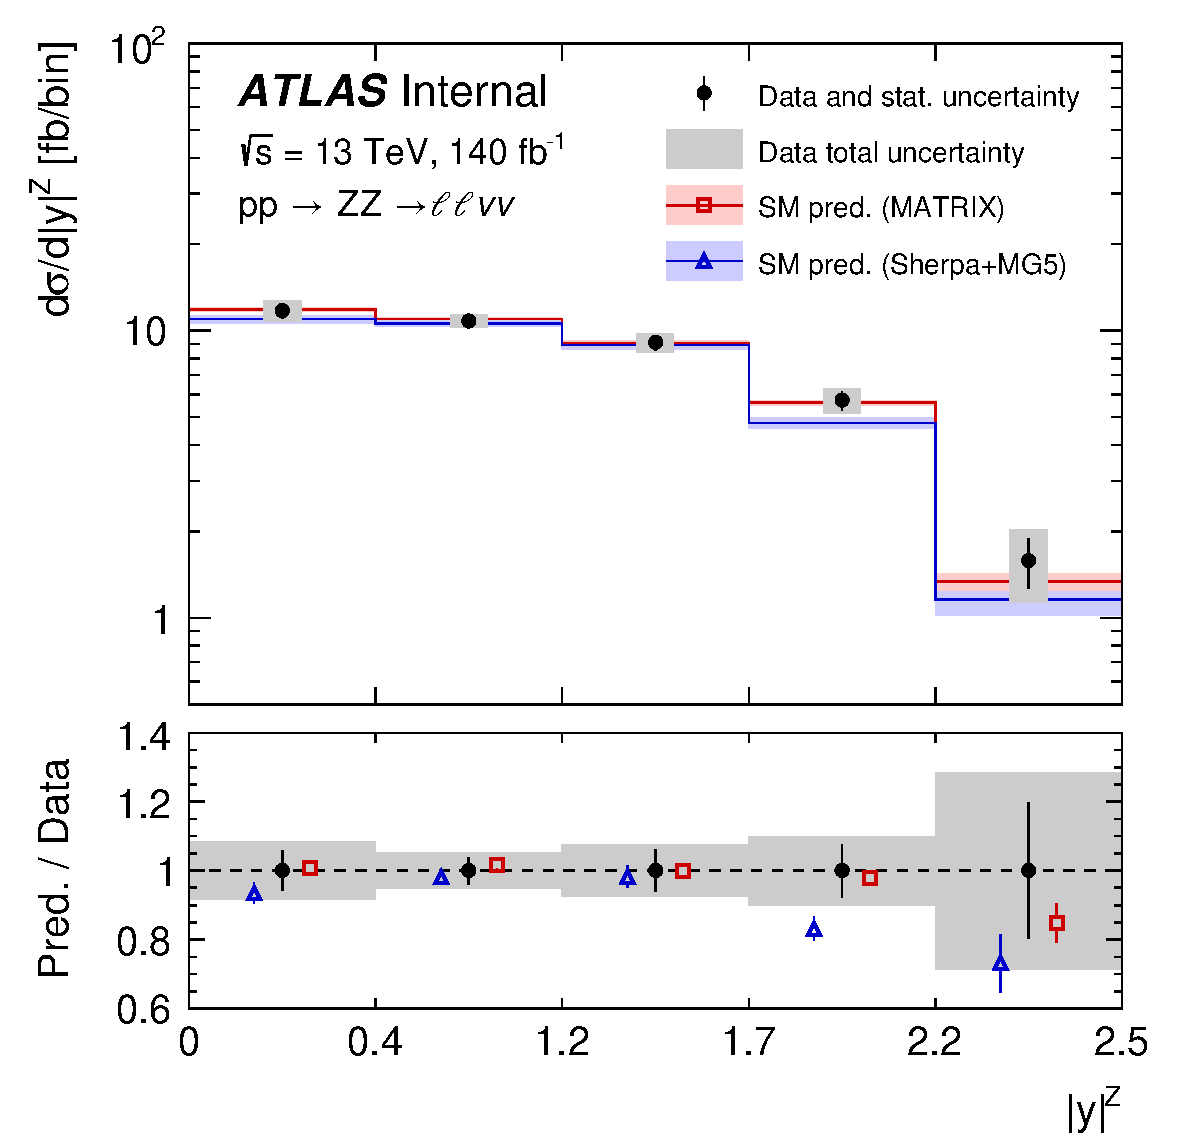
\includegraphics[width=0.32\linewidth]{figures/ch5-llvv/diff-xs/ZZ-y_Z.pdf}
    }
    \subfloat[]{    
    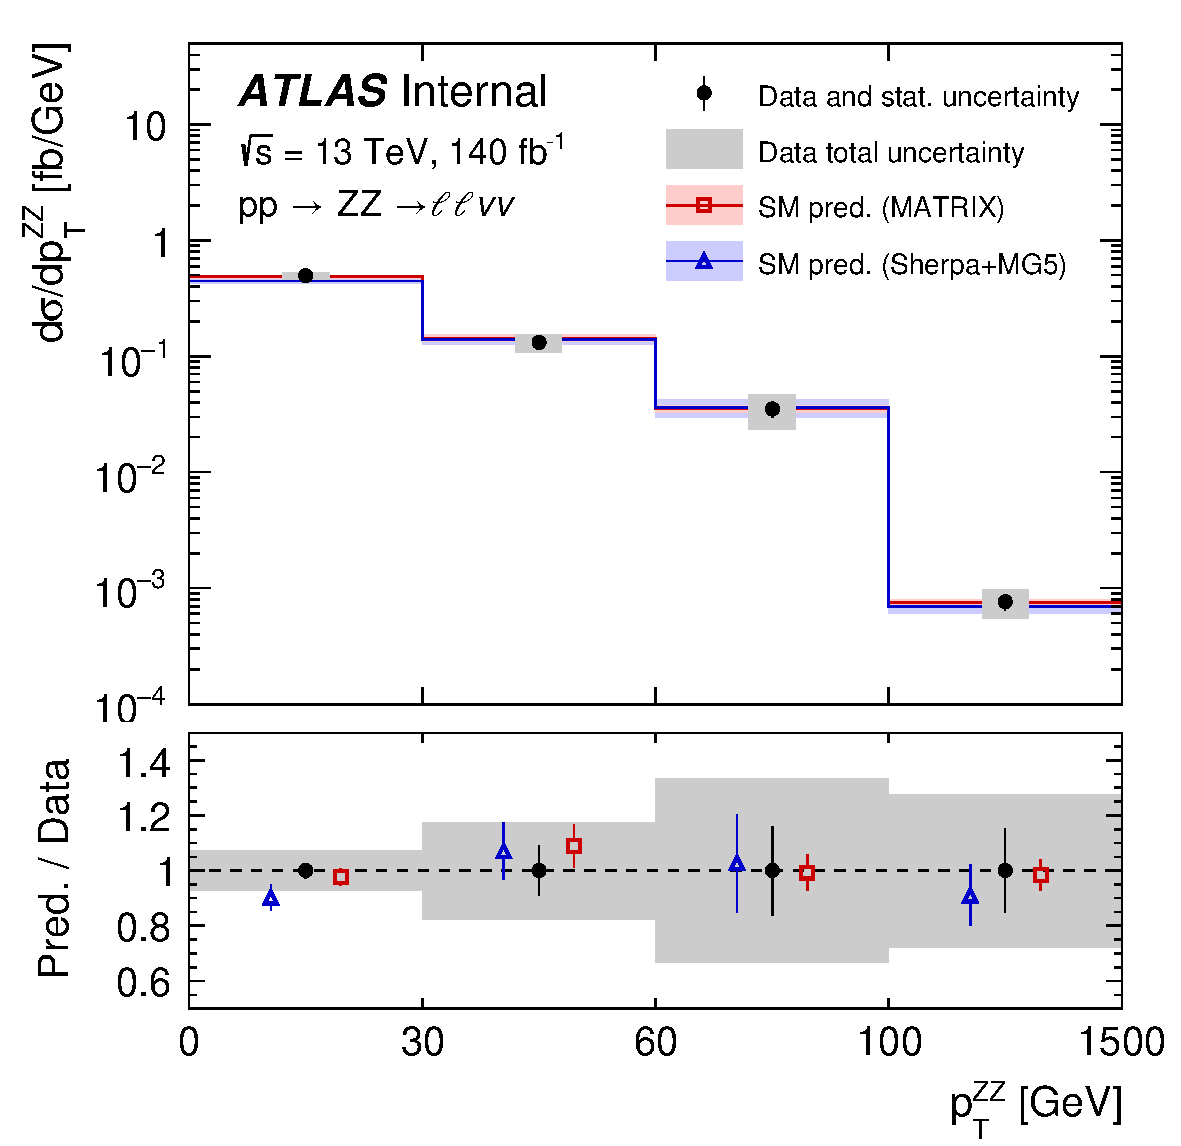
\includegraphics[width=0.32\linewidth]{figures/ch5-llvv/diff-xs/ZZ-pT_ZZ.pdf}
    }
    \subfloat[]{    
    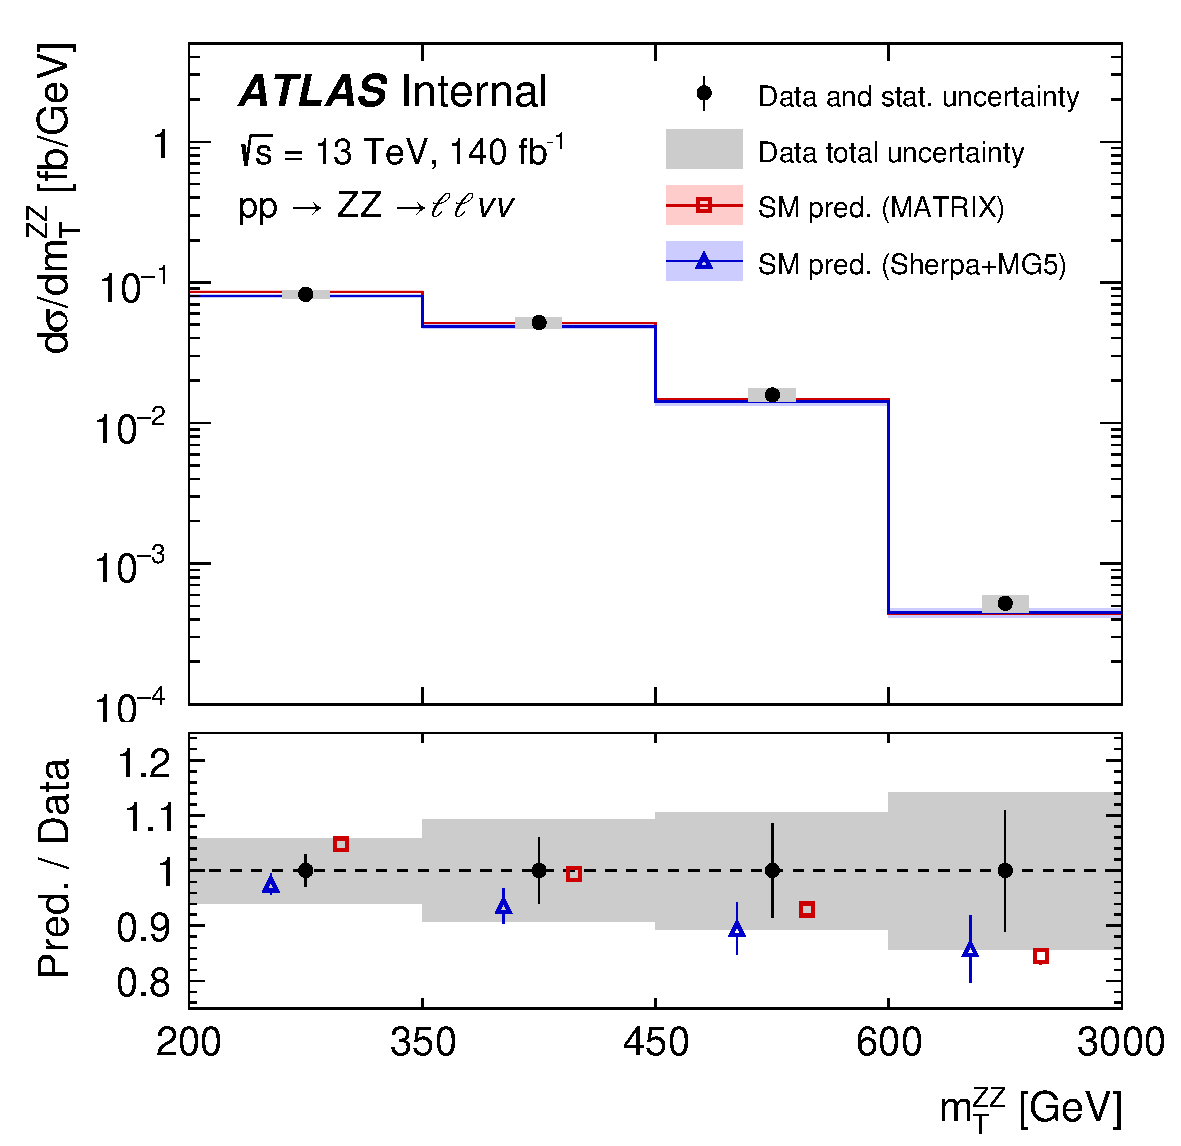
\includegraphics[width=0.32\linewidth]{figures/ch5-llvv/diff-xs/ZZ-mT_ZZ.pdf}
    }\\
    \subfloat[]{    
    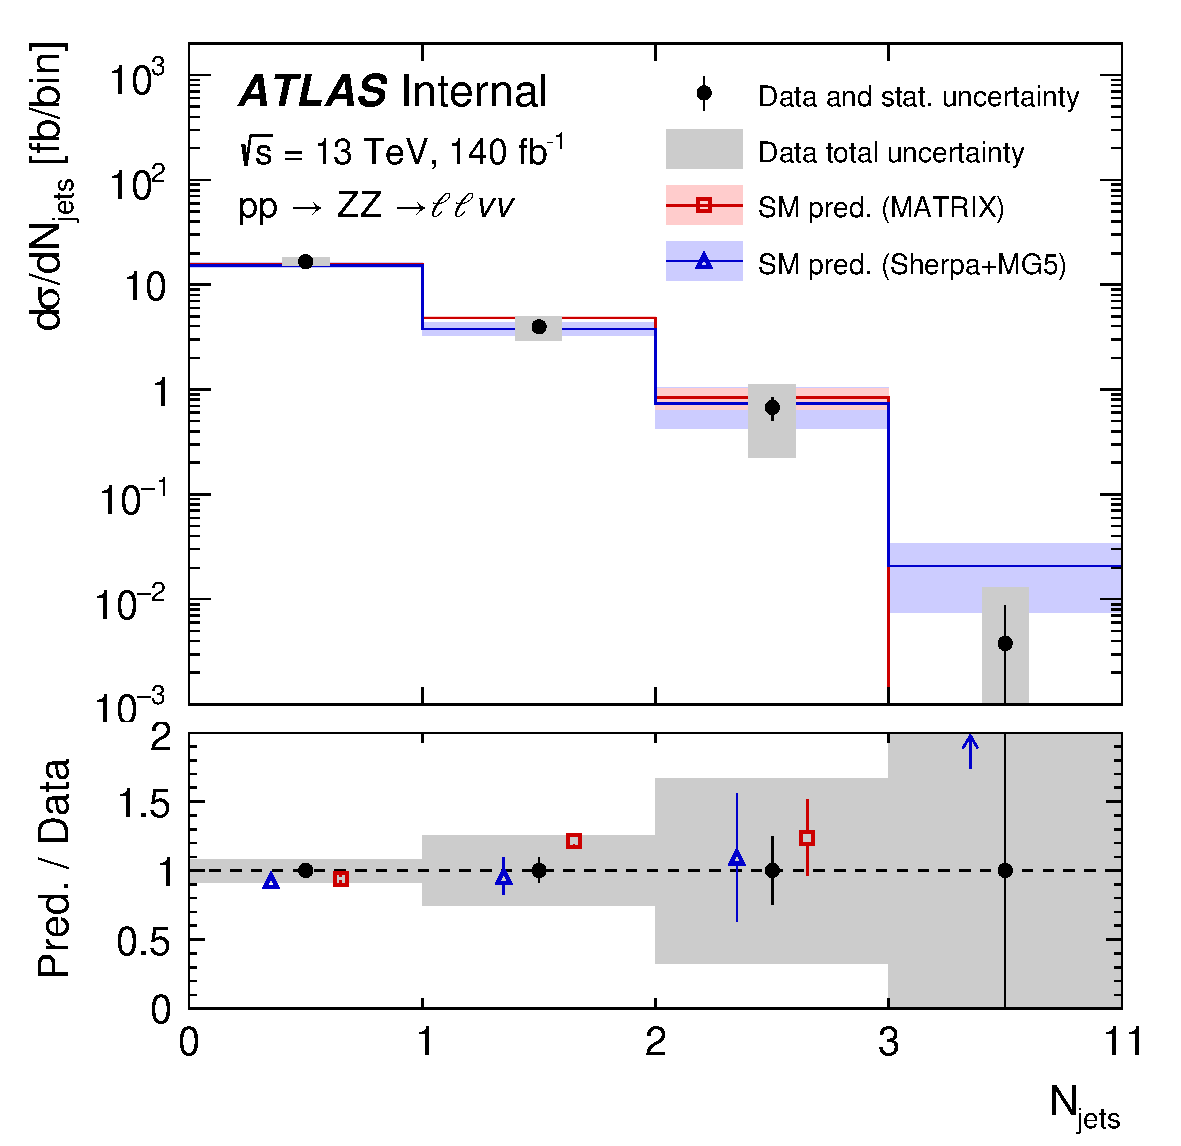
\includegraphics[width=0.32\linewidth]{figures/ch5-llvv/diff-xs/ZZ-njets.pdf} 
    }
    \subfloat[]{    
    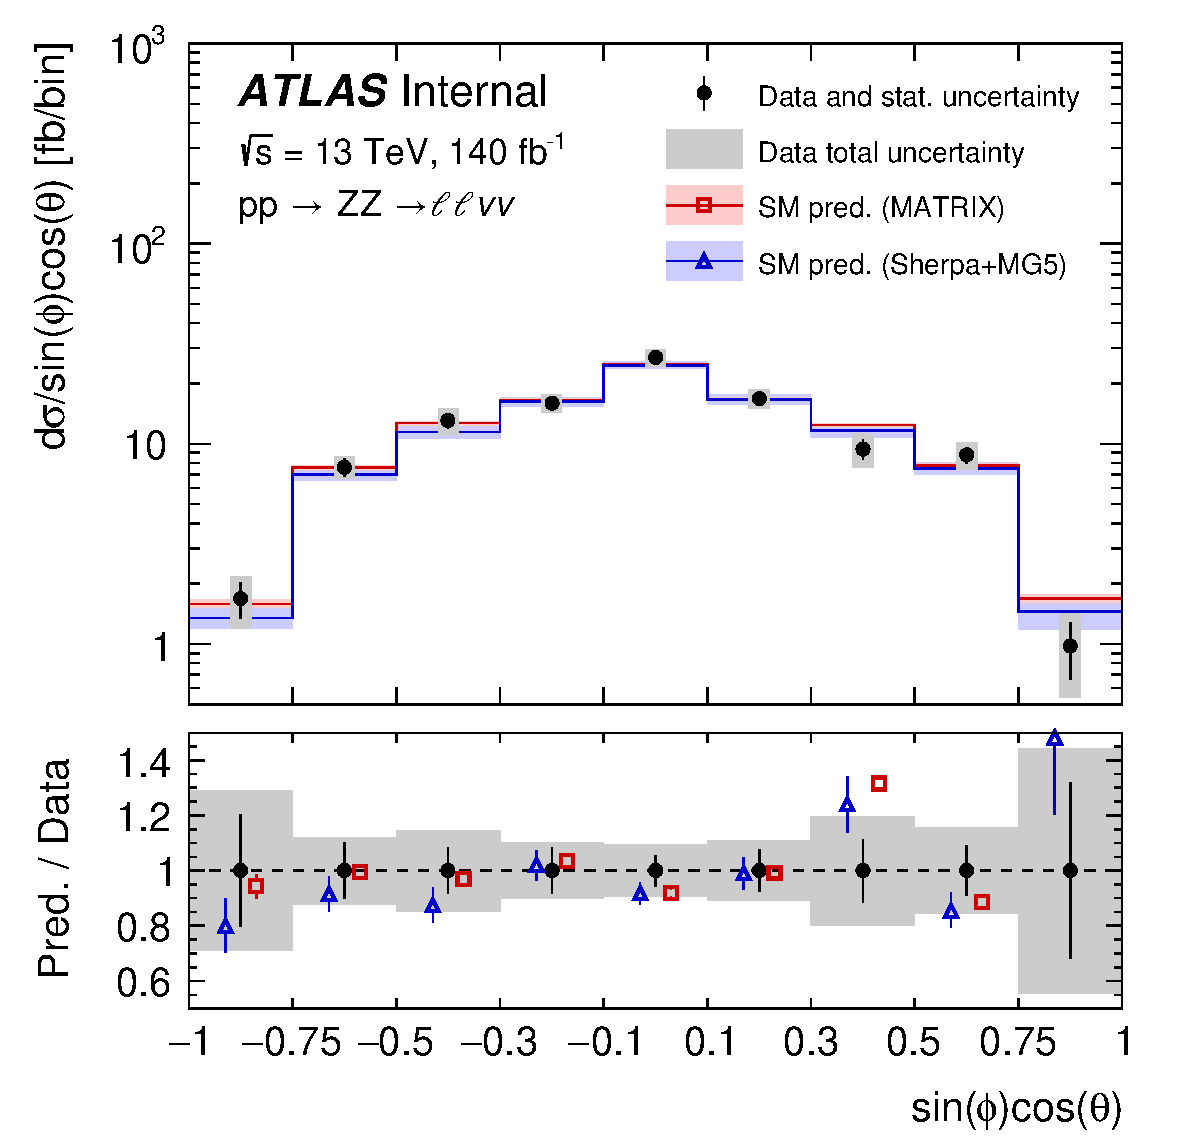
\includegraphics[width=0.32\linewidth]{figures/ch5-llvv/diff-xs/ZZ-sincos_2.pdf}
    }
    \caption{Differential cross-section measurements in the inclusive $ZZ\rightarrow \ell\ell\nu\nu$ fiducial phase space, compared with MC predictions calculated by the nominal \textsc{Sherpa} simulation %(denoted as \textsc{Sherpa})
    and by \textsc{Matrix} for a set of kinematic variables:
(a) $p_\text{T}^\text{leading lepton}~,
\text{(b)}~ p_\text{T}^\text{Z}~,
\text{(c)}~\Delta\phi(\ell, \ell),~
\text{(d)}~|y^Z|,~
\text{(e)}~ p_\text{T}^\text{ZZ},~
\text{(f)}~ m_\text{T}^\text{ZZ},~
\text{(g)}~ N_\text{jets}$,
and (h) a CP-sensitive angular variable, $\sin(\varphi)\cos(\theta)$.
The statistical and total uncertainties on the data points are displayed in both the differential cross-sections and the corresponding ratios. The total theoretical uncertainties for the \textsc{Sherpa} and \textsc{Matrix} predictions are represented as shaded bands in the cross-section panels and as error bars in the ratio panels.
}
\label{fig:diff-xs-ZZ}
\end{figure}


\begin{figure}[!hbtp]
    \centering
    \subfloat[]{  
    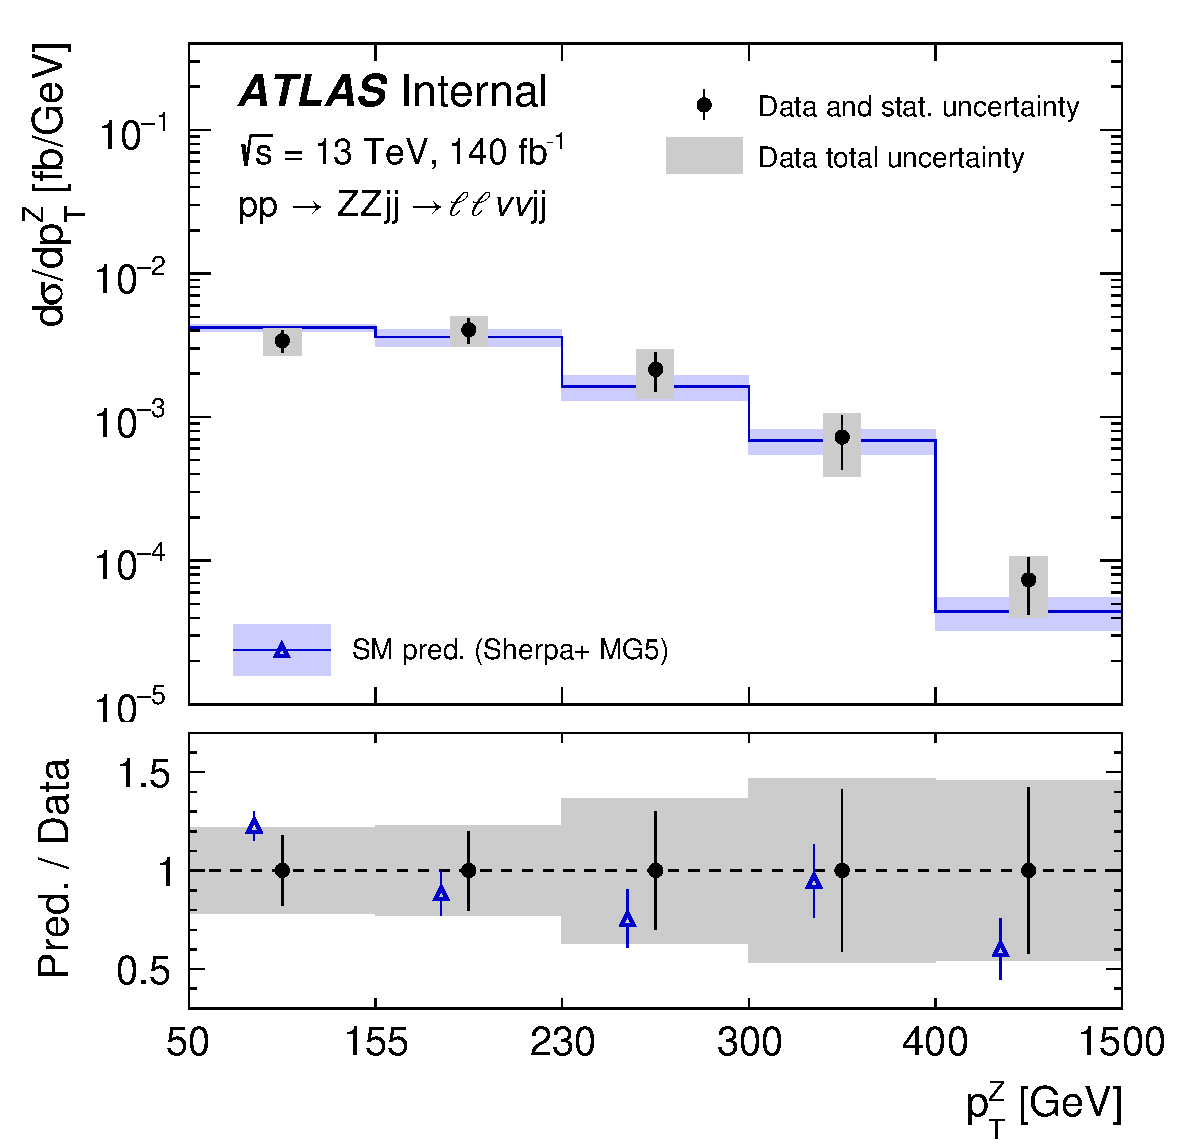
\includegraphics[width=0.32\linewidth]{figures/ch5-llvv/diff-xs/ZZjj-pT-Z.pdf}
    }
    \subfloat[]{  
    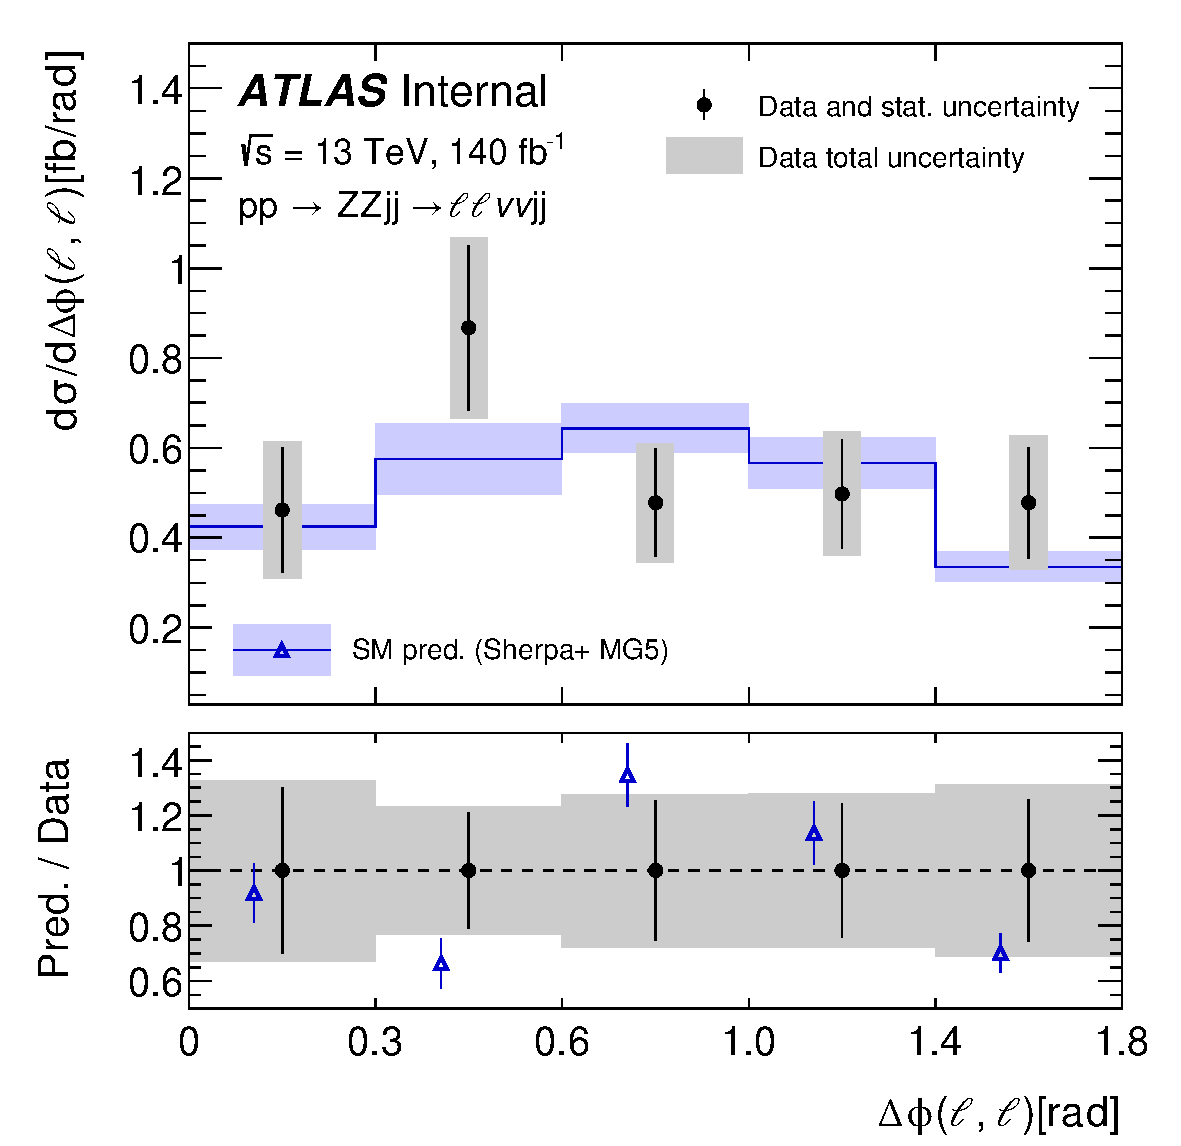
\includegraphics[width=0.32\linewidth]{figures/ch5-llvv/diff-xs/ZZjj-Dphi-ll.pdf}
    }
    \subfloat[]{  
    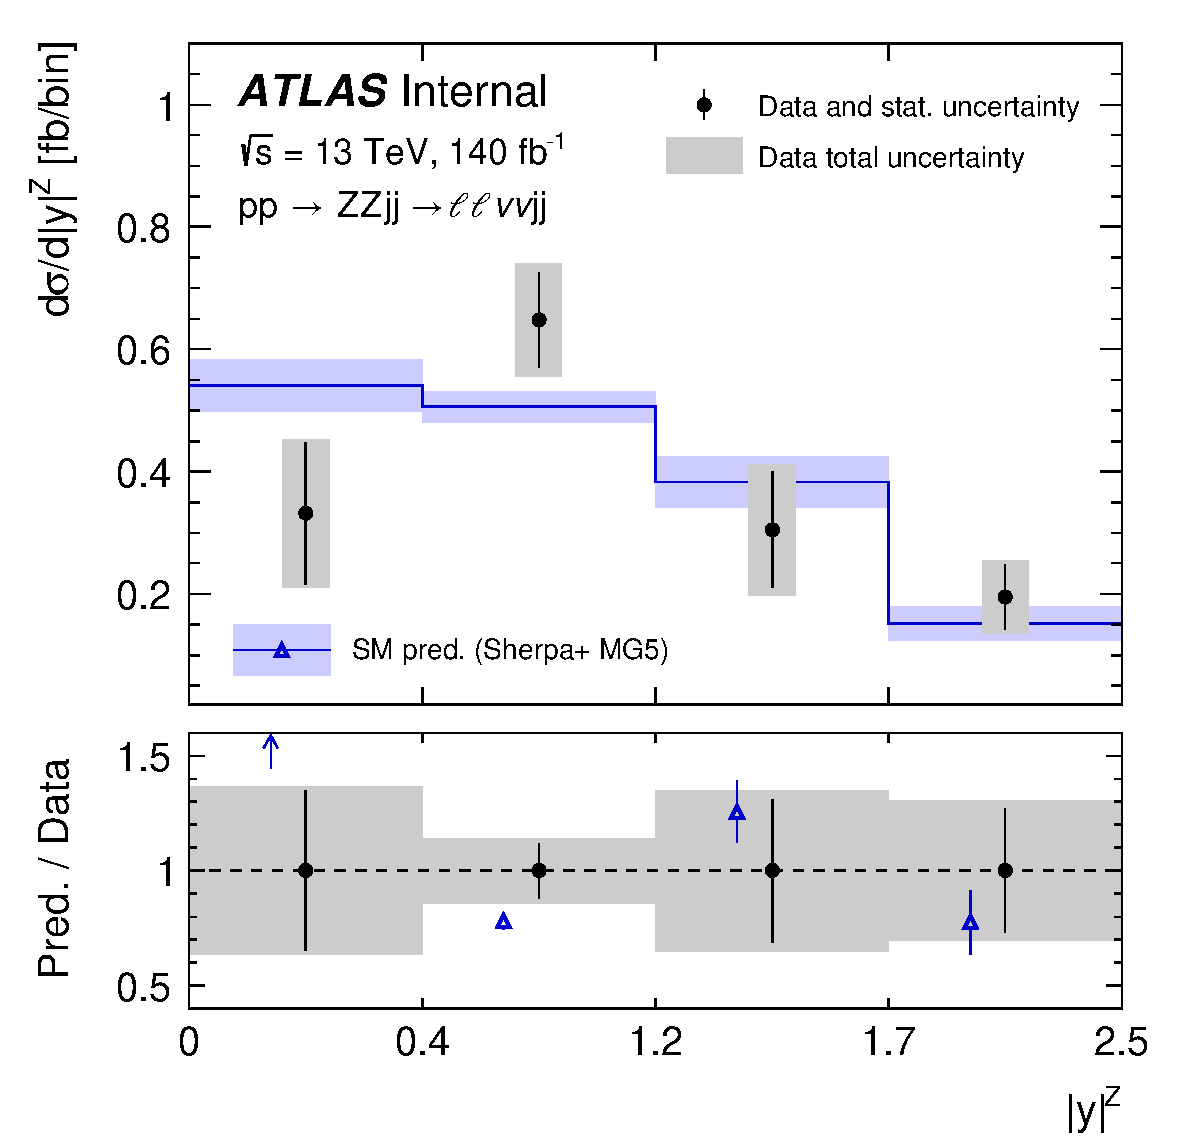
\includegraphics[width=0.32\linewidth]{figures/ch5-llvv/diff-xs/ZZjj-Y-Z.pdf}
    }\\
    \subfloat[]{      
    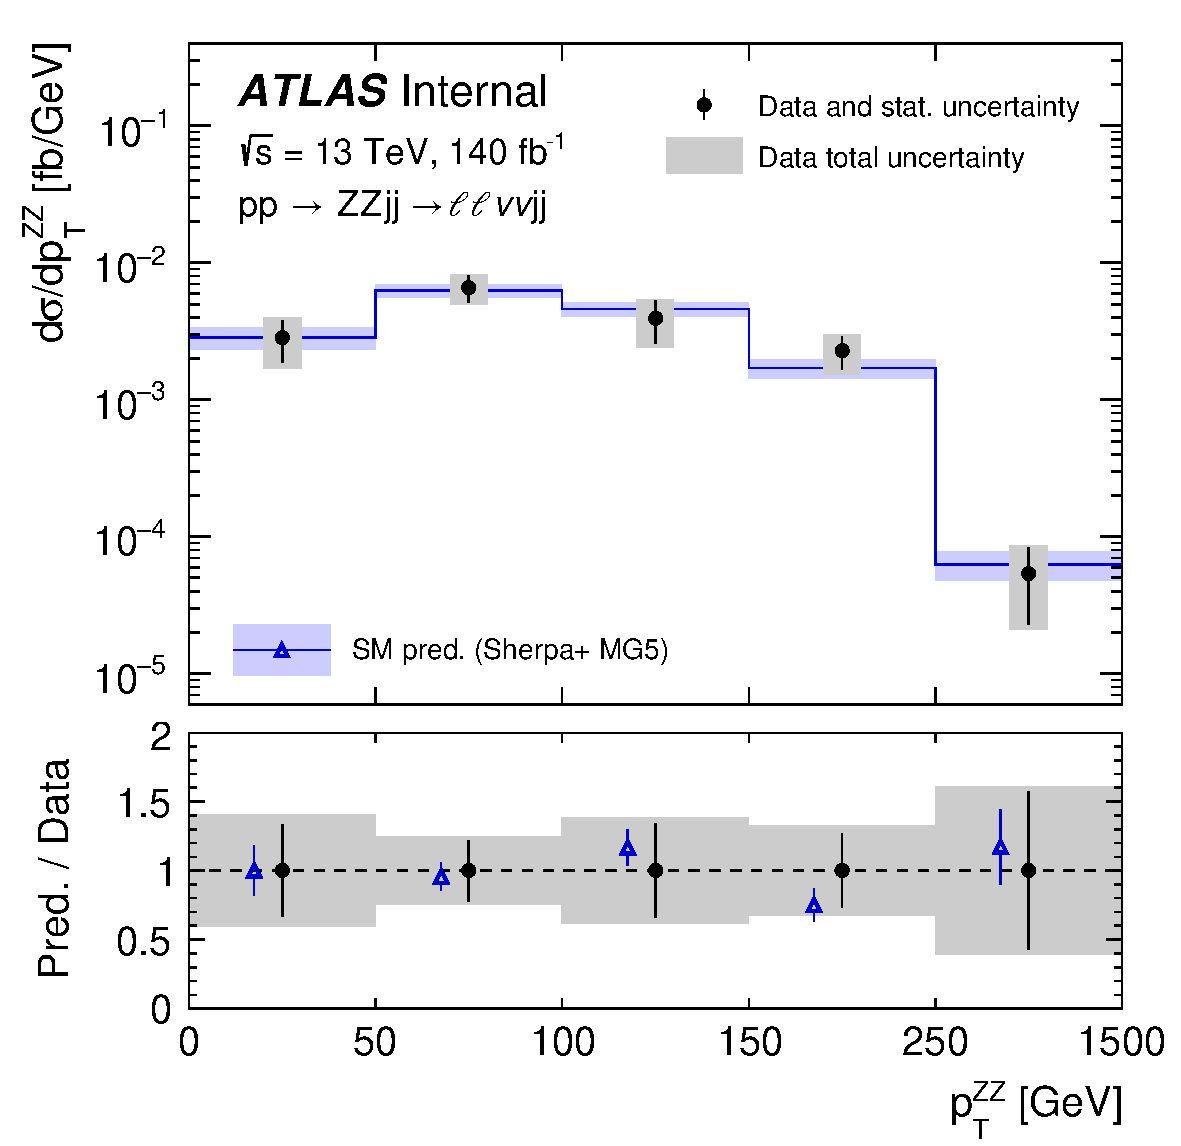
\includegraphics[width=0.35\linewidth]{figures/ch5-llvv/diff-xs/ZZjj-pT-ZZ.pdf}
    }
    \subfloat[]{      
    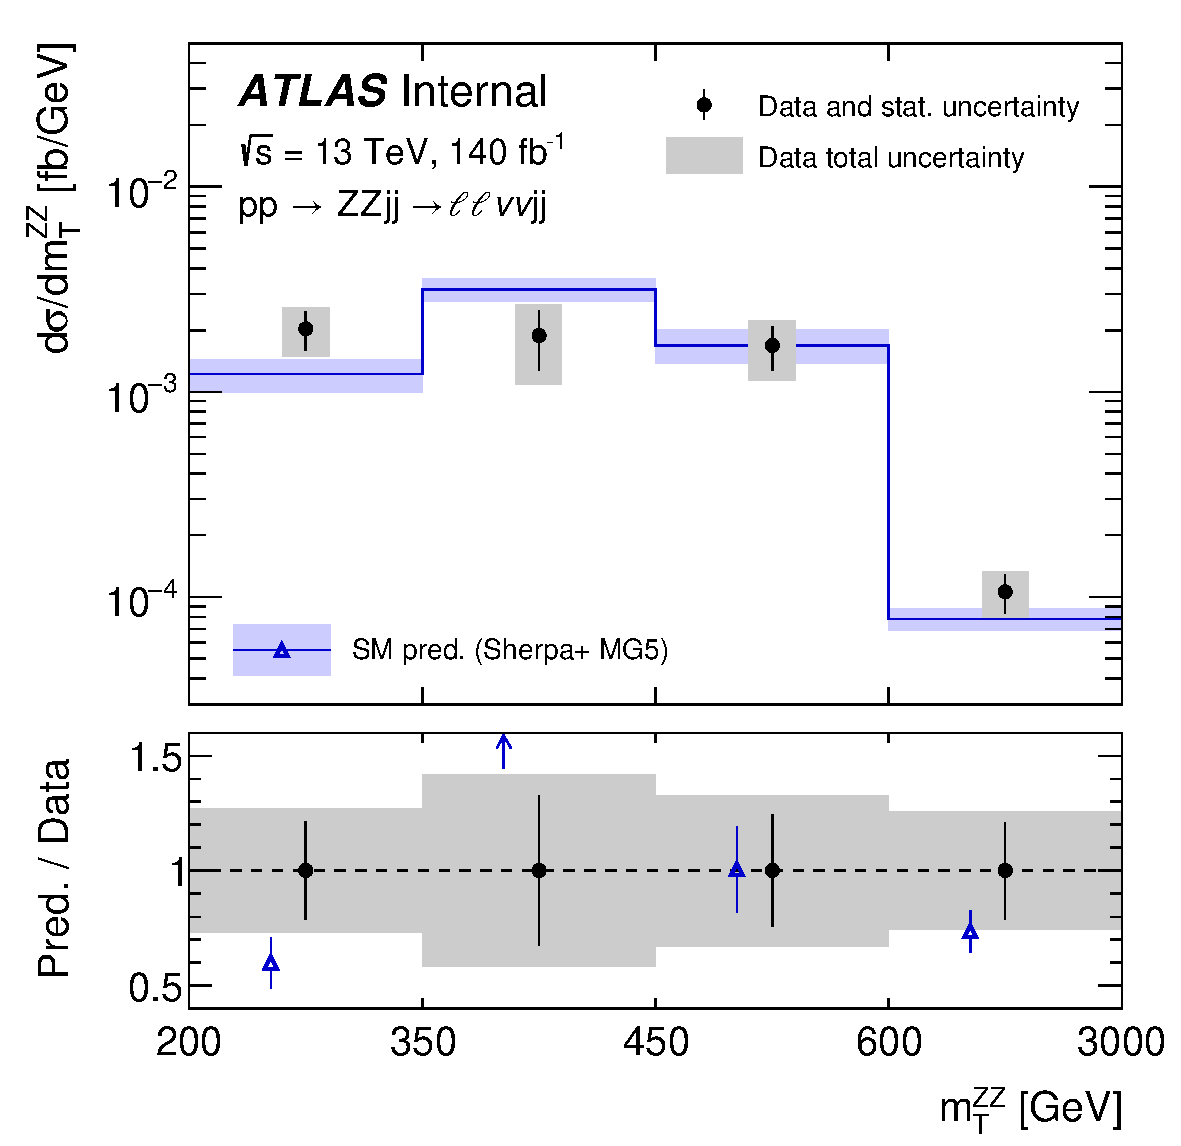
\includegraphics[width=0.35\linewidth]{figures/ch5-llvv/diff-xs/ZZjj-mT-ZZ.pdf}
    }\\
            \subfloat[]{  
    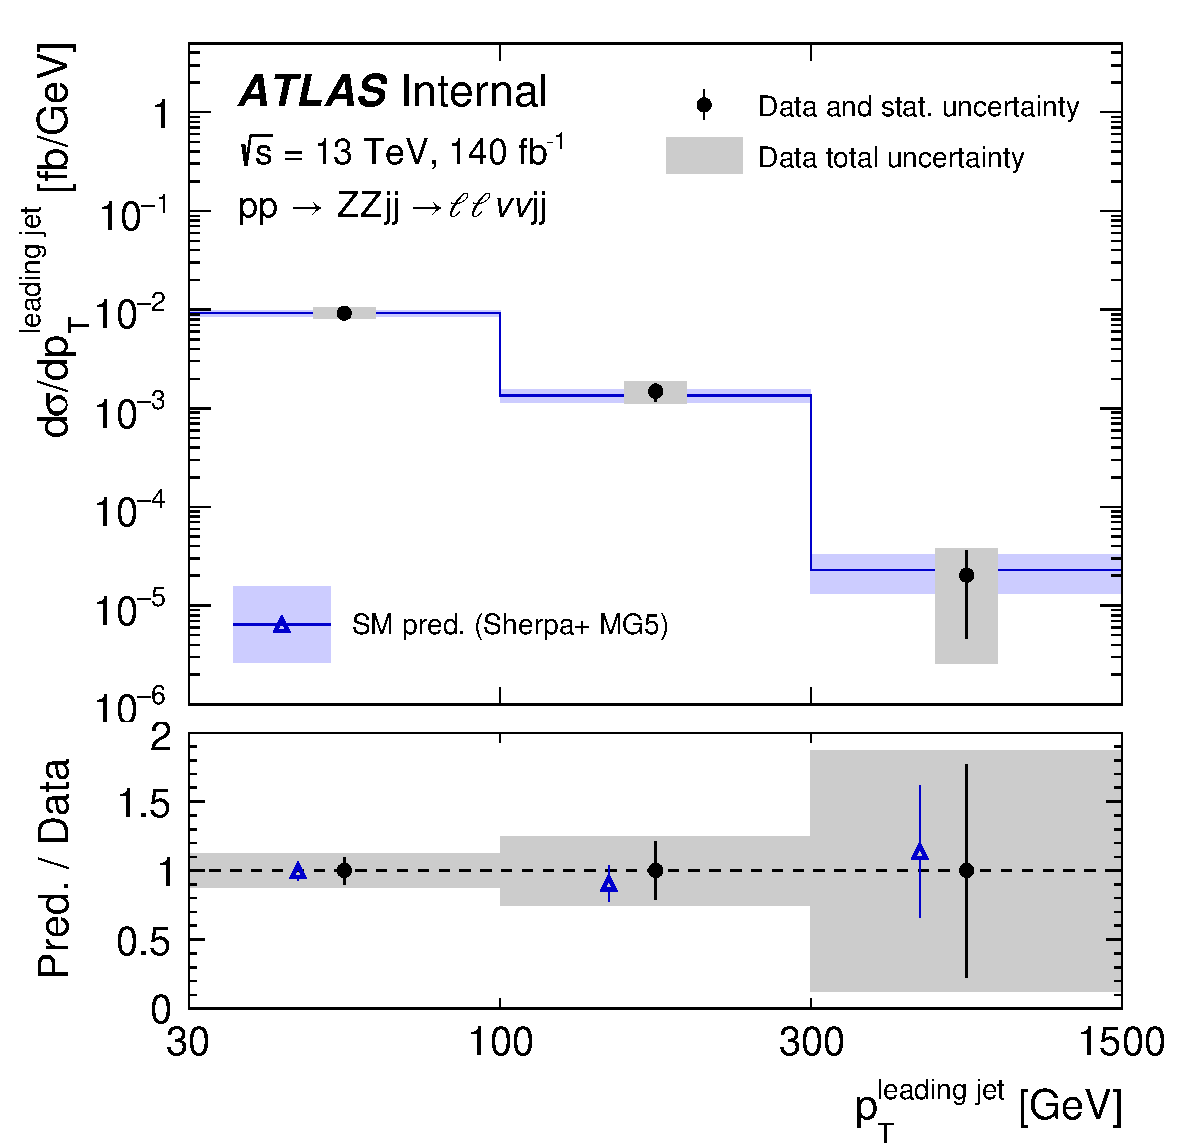
\includegraphics[width=0.35\linewidth]{figures/ch5-llvv/diff-xs/ZZjj-pT-j1.pdf}
    }
            \subfloat[]{  
    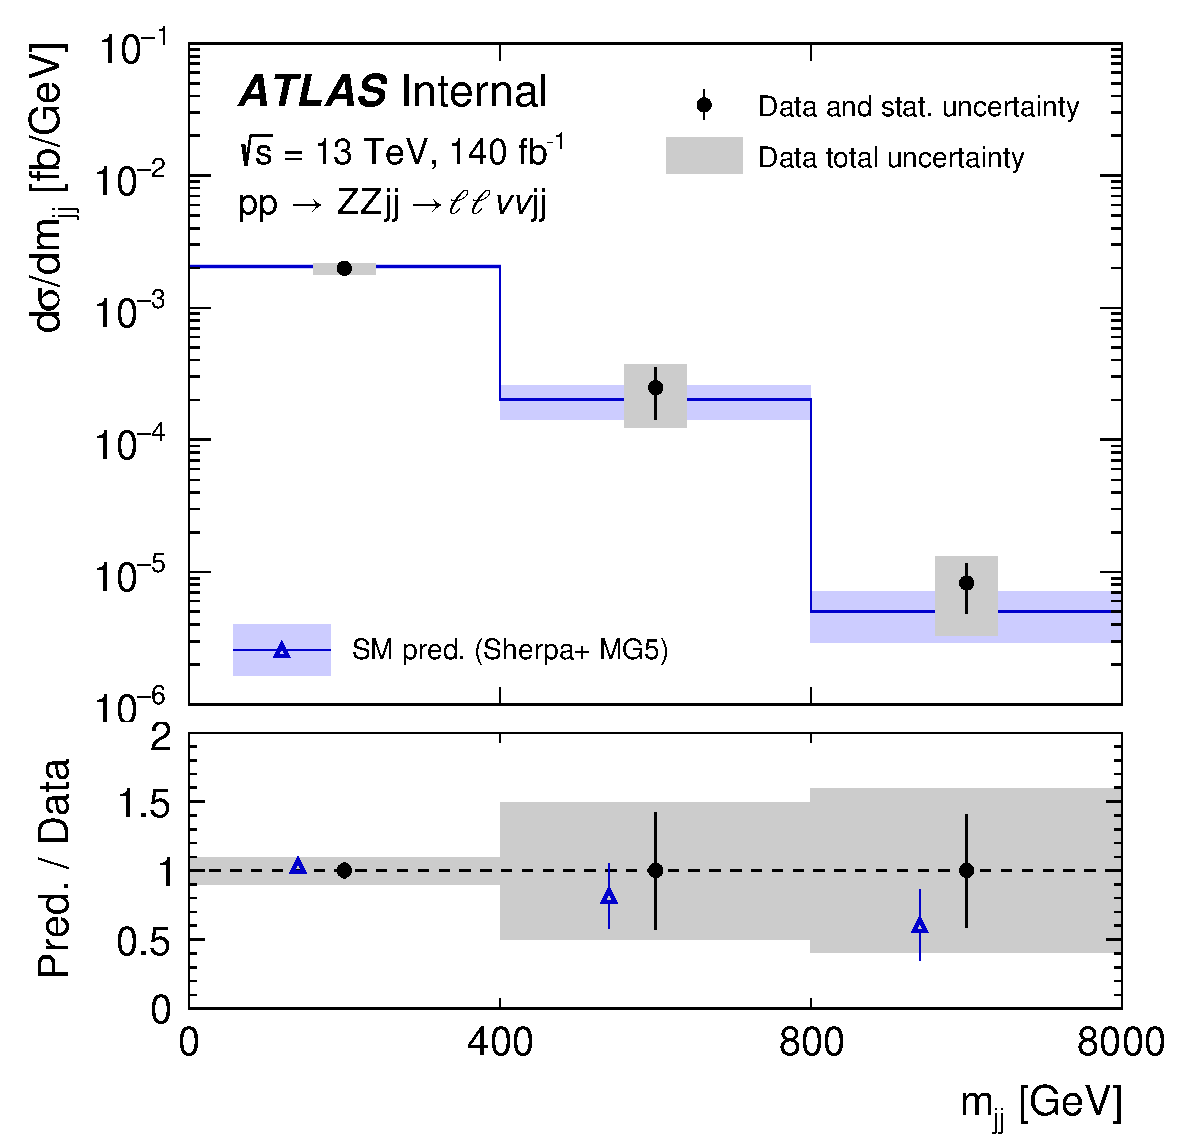
\includegraphics[width=0.35\linewidth]{figures/ch5-llvv/diff-xs/ZZjj-mjj.pdf}
    }
    \caption{Differential cross-section measurements in the $ZZjj \rightarrow \ell\ell\nu\nu jj$ fiducial phase space, compared with SM predictions for a set of kinematic variables:
     $ \text{(a)}~p_\text{T}^\text{Z},~
       \text{(b)}~\Delta\phi(\ell, \ell),~
       \text{(c)}~|y^Z|,~
       \text{(d)}~p_\text{T}^\text{ZZ},~
       \text{(e)}~m_\text{T}^\text{ZZ},~
       \text{(f)}~p_\text{T}^\text{leading-jet},~
       \text{and} ~\text{(g)}~m_\text{jj}.   
    $ 
     The SM predictions are obtained using \textsc{Sherpa} for strong production and \textsc{MadGraph5} for electroweak production. 
     The statistical and total uncertainties on the data points are displayed in both the differential cross-sections and the corresponding ratios. The total theoretical uncertainties for the  MC predictions are represented as shaded bands in the cross-section panels and as error bars in the ratio panels.
    }
\label{fig:diff-xs-ZZjj}
\end{figure}



%%%%%%%%%%%%%%%%%%%%%%%%%%%%%%%%%%%%%%%%%%%%%%%%%%
%\section{Results}
%\label{sec:llvv_results}

%This section presents the results of the inclusive $ZZ \to \ell\ell\nu\nu$ analysis performed on the full Run 2 dataset, corresponding to an integrated luminosity of $140~\text{fb}^{-1}$. The measurements include the extraction of signal strengths via a profile-likelihood fit, the determination of fiducial and total integrated cross-sections, and the measurement of differential cross-sections unfolded to particle level. Finally, limits are placed on anomalous neutral triple gauge couplings (aTGCs) within the Effective Field Theory (EFT) framework.

%\subsection{Signal Extraction and Fit Results}
%\label{subsec:signal_extraction}

%The signal yield is extracted using a binned profile-likelihood fit to the discriminative observable $\Delta\phi(\ell\ell, E_{\mathrm{T}}^{\text{miss}})$. This fit is performed simultaneously across the Signal Region (SR) and the dedicated Control Regions (CRs) described in Section~\ref{sec:llvv_event_selection}. 

%The observed signal strength parameter, defined as the ratio of the observed signal yield to the Standard Model (SM) prediction ($\mu = \sigma_{\text{obs}}/\sigma_{\text{exp}}$), is measured to be:
%\begin{equation}
%    \mu_{ZZ} = 1.05 \pm 0.05,
%\end{equation}
%indicating excellent agreement with the SM expectation. The dominant background normalization factors constrained by the fit are found to be close to unity, with $\mu_{WZ} = 1.00^{+0.06}_{-0.05}$ and $\mu_{\text{top}} = 0.98^{+0.13}_{-0.10}$. The normalization for the $Z+\text{jets}$ background varies by jet multiplicity, ranging from $1.14$ in the 0-jet region to $1.10$ in the $\geq 2$-jet region.

%The post-fit distribution of $\Delta\phi(\ell\ell, E_{\mathrm{T}}^{\text{miss}})$ in the signal region is shown in Figure~\ref{fig:postfit_observed}. The data is well-described by the post-fit predictions within the assigned uncertainties. Representative kinematic distributions, such as the transverse mass of the $ZZ$ system ($m_{\mathrm{T}}^{ZZ}$) and the transverse momentum of the leading lepton, are shown in Figure~\ref{fig:postfit_observed}.

%\begin{figure}[!htbp]
%    \centering
%    \subfloat[]{
%        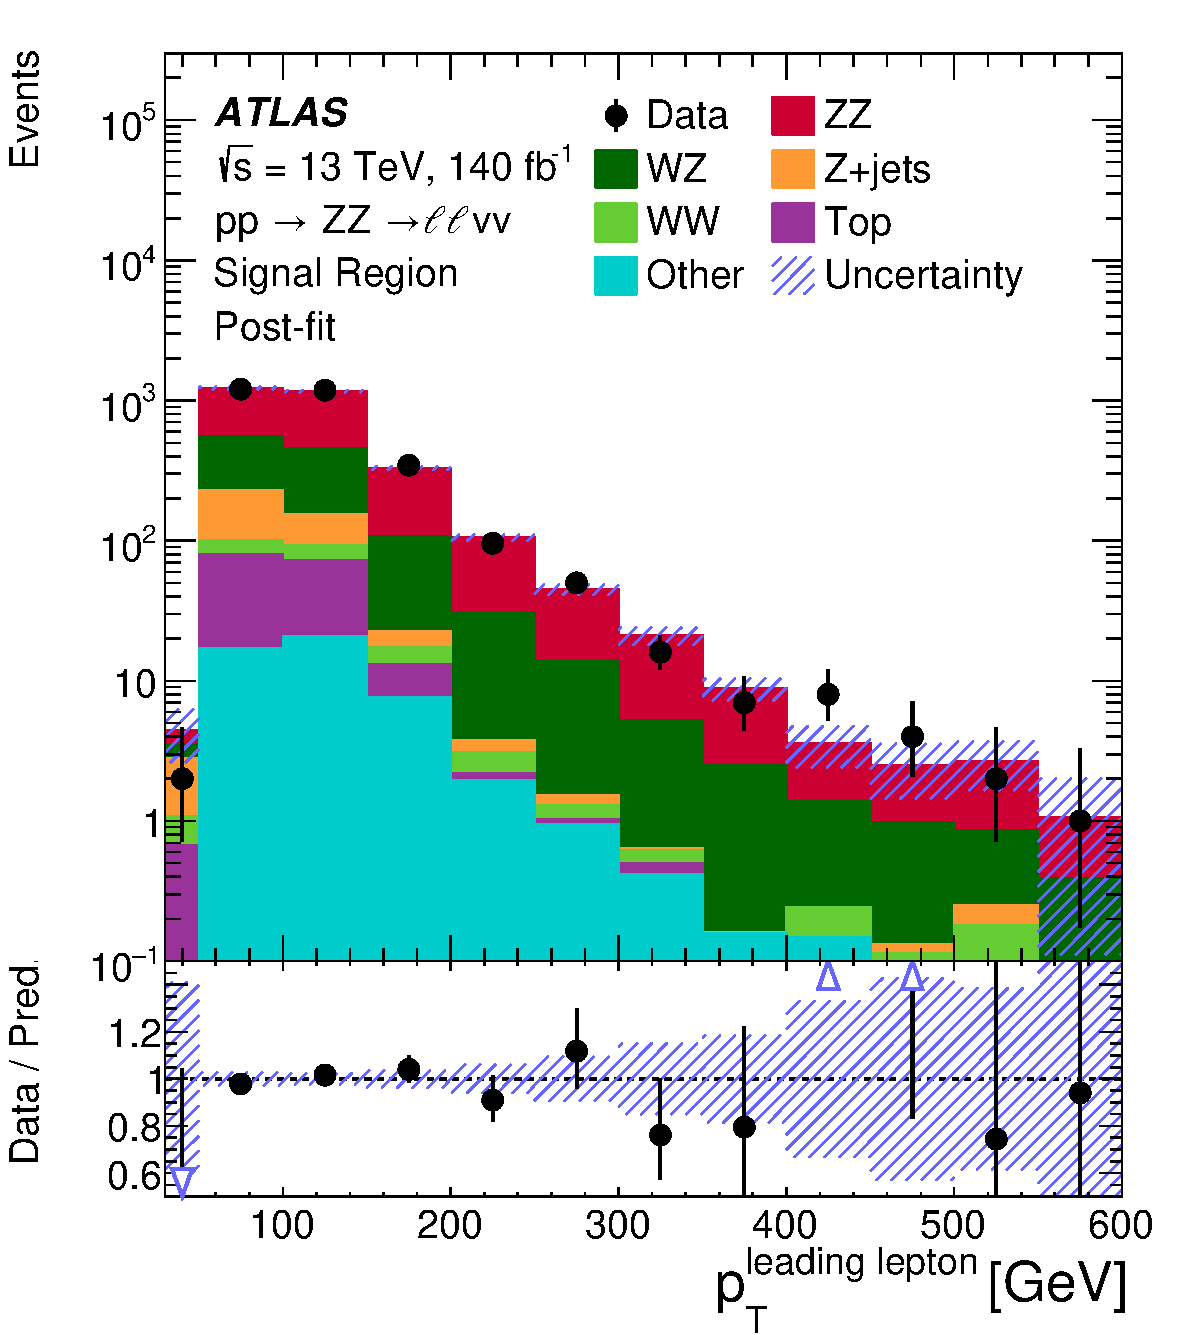
\includegraphics[width=0.3\linewidth]{figures/ch5-llvv/fig_postfit_a.pdf}
%        \label{fig:postfit_leading_lep_pt}
%    }
%    \hfill
%    \subfloat[]{
%        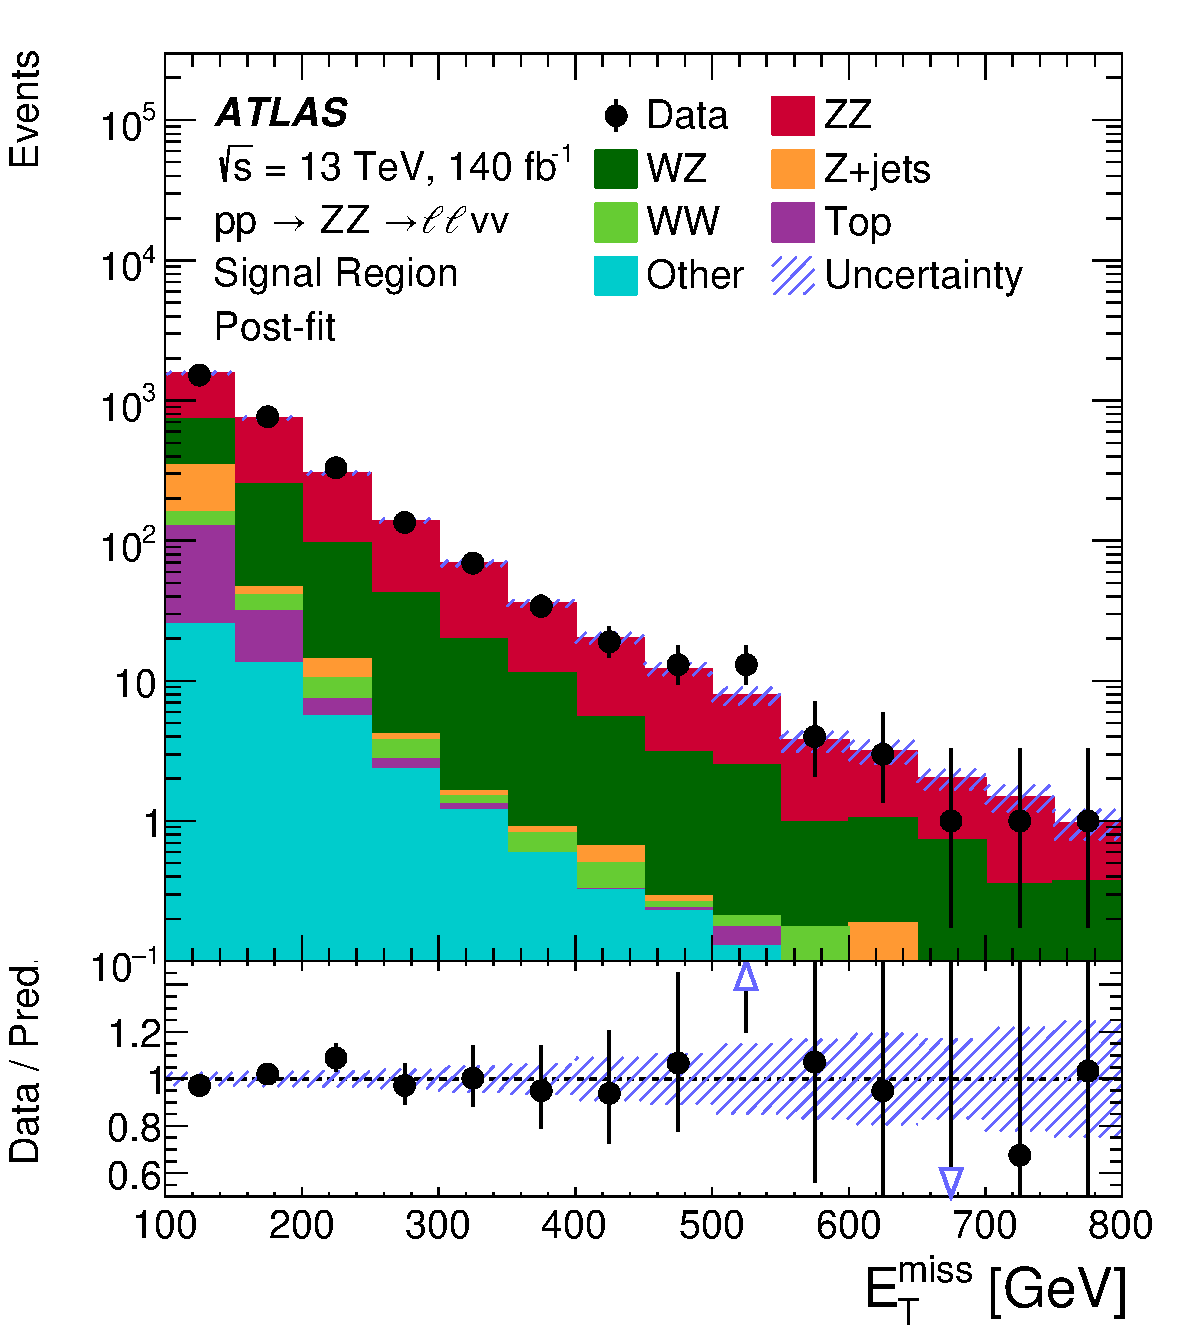
\includegraphics[width=0.3\linewidth]{figures/ch5-llvv/fig_postfit_b.pdf}
%        \label{fig:postfit_met}
%    }
%    \hfill
%    \subfloat[]{
%        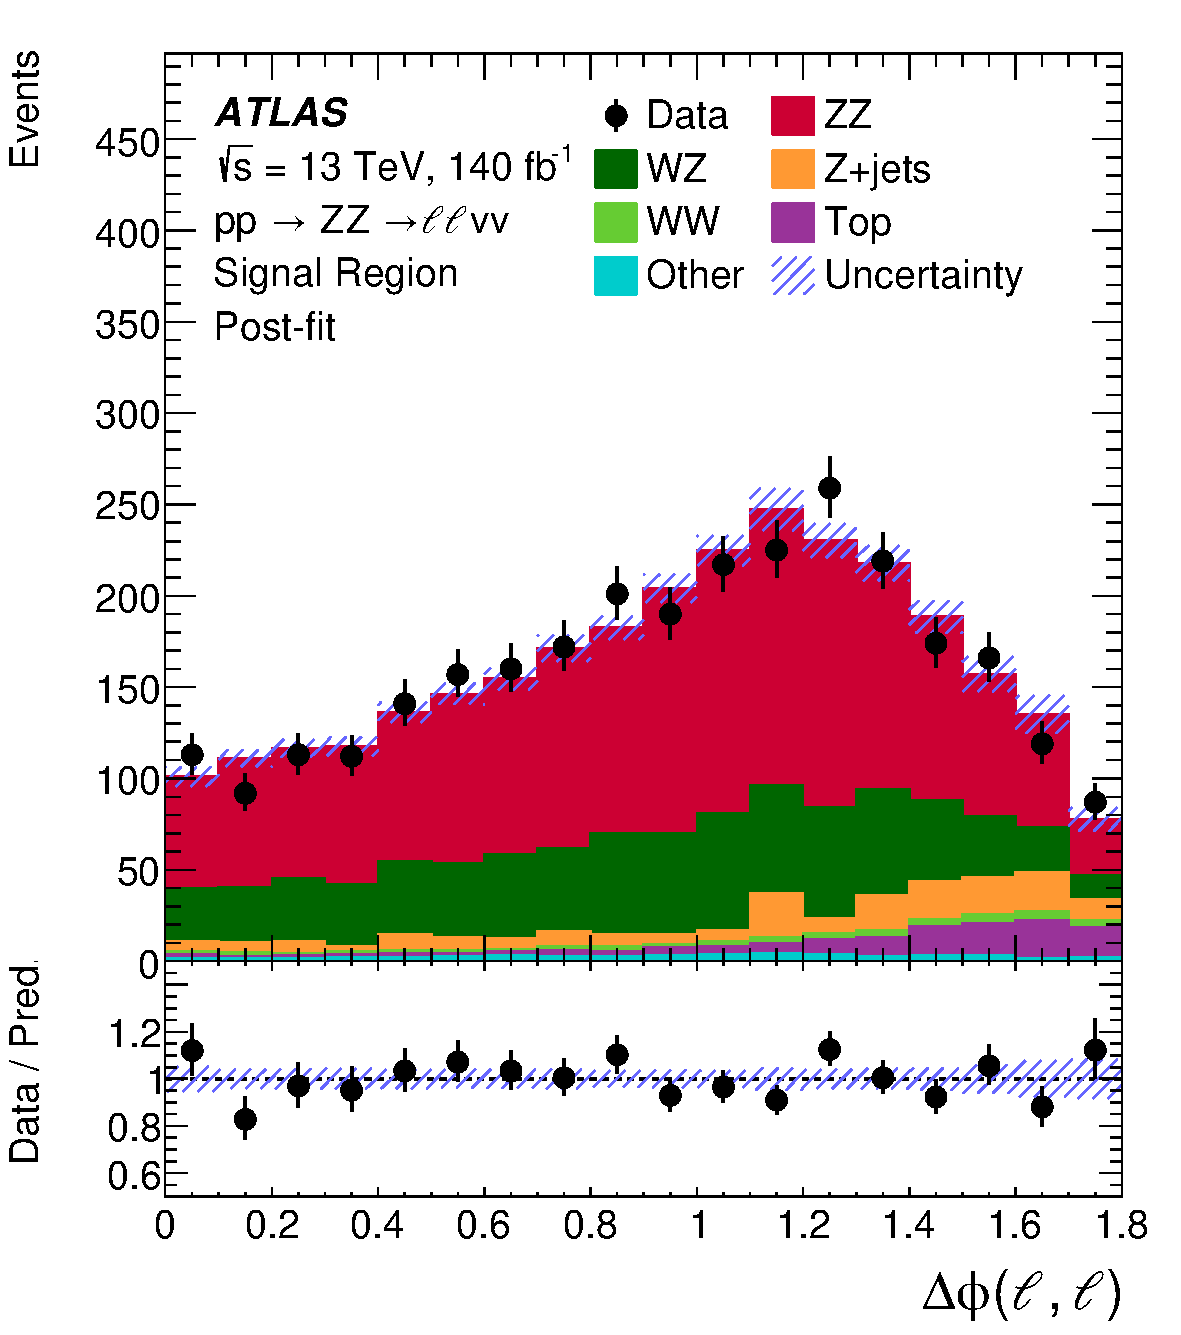
\includegraphics[width=0.3\linewidth]{figures/ch5-llvv/fig_postfit_c.pdf}
%        \label{fig:postfit_dphi_ll}
%    }    
%    \caption{Post-fit kinematic distributions for the inclusive $ZZ$ SR
%    (a) the transverse momentum of the leading lepton $p_\text{T}^\text{leading lepton}$, 
%    (b) $E_\text{T}^\text{miss}$, and 
%    (c) the azimuthal angle separation between two charged leptons $\Delta\phi(\ell, \ell)$. 
%    The data points are shown with statistical error bars, while the shaded band represents the total post-fit uncertainty in the prediction, combining statistical and systematic uncertainties. Open markers indicate data points lying outside the vertical range of the plot.}
%    \label{fig:postfit_observed}
%\end{figure}

%\subsection{Integrated Cross-Section Measurements}
%\label{subsec:integrated_xsec}

%The measured signal strength is converted into a fiducial cross-section using the SM predictions from \textsc{Sherpa} and \textsc{MadGraph5}. 

%The measured fiducial cross-section for the inclusive $ZZ \to \ell\ell\nu\nu$ process is:
%%    \sigma_{ZZ \to \ell\ell\nu\nu}^{\text{fid}} = 21.0 \pm 1.0~\text{fb}.
%\end{equation}
%The total uncertainty is composed of $\pm 0.73$ (stat), $\pm 0.57$ (exp), $\pm 0.18$ (theory), and $\pm 0.18$ (lumi) fb. This result represents a significant improvement in precision compared to previous ATLAS measurements using partial Run 2 data, with the total uncertainty reduced from 7.0\% to approximately 4.8\%. 

%The measurement is consistent with the state-of-the-art SM prediction calculated using \textsc{Matrix} at NNLO in QCD and NLO in EW corrections, which yields $21.03 \pm 0.30$ fb.

%Using the fiducial acceptance factor $A_{ZZ}$ and the branching ratio for $ZZ \to 2\ell 2\nu$, the result is extrapolated to the full phase space for $Z$ boson masses between 66 and 116 GeV. The total $pp \to ZZ$ cross-section is determined to be:
%\begin{equation}
%    \sigma_{pp \to ZZ}^{\text{total}} = 15.38 \pm 0.81~\text{pb},
%\end{equation}
%which agrees well with the \textsc{Matrix} prediction of $15.40 \pm 0.38$ pb.


\section{Constraints on Anomalous Gauge Boson Self-interaction Couplings}
\label{subsec:anom_couplings}

As presented in the sections above, the measured fiducial and total cross-sections are in good agreement with the SM predictions within the measurement uncertainties. These results enable constraints to be placed on anomalous gauge boson self-interaction couplings.

Inclusive $ZZ$ production (particularly see diagram in Figure~\ref{fig:zz-prod} (c)) provides a key channel for probing anomalous neutral triple gauge couplings (aNTGCs). In the SM, the $s$-channel diagram involving the neutral $ZZZ$ or $ZZ\gamma$ vertex is absent, making this process particularly sensitive to possible deviations from SM expectations.

The $ZZjj$ production in $pp$ collisions (see Figure~\ref{fig:zzjj-prod}) includes electroweak vector boson scattering (VBS) processes that involve the triple gauge boson ($WWZ$) and quartic gauge boson ($WWZZ$) couplings. These processes are directly linked to two fundamental aspects of the SM electroweak theory, the non-Abelian gauge structure and spontaneous electroweak symmetry breaking, and therefore provide sensitivity to both anomalous triple gauge couplings (aTGCs) and anomalous quartic gauge couplings (aQGCs).

Since no unified framework simultaneously describing aTGCs and aQGCs is currently available, the inclusive $ZZ$ measurement is used to constrain aTGCs, while the $ZZjj$ process is used to search for aQGCs.

Simulation samples for aTGC and aQGC interpretations are generated using the decomposition method, in which the matrix element is expressed as
\begin{equation}
\small
    |A_{\text{SM}} + \sum_i c_i A_i|^2
    = |A_{\text{SM}}|^2
    + \sum_i c_i\, 2\, \mathrm{Re}(A_{\text{SM}} A_i^*)
    + \sum_i c_i^2 |A_i|^2
    + \sum_{i \ne j} c_i c_j\, 2\, \mathrm{Re}(A_i A_j^*),
\end{equation}\label{eq:BSM}
where $A_{\text{SM}}$ denotes the SM amplitude, $A_i$ the beyond-the-SM (BSM) contributions, and $c_i$ the corresponding coupling coefficients. 
The first term represents the pure SM contribution. The second term corresponds to the interference between the SM and each BSM amplitude (linear term), while the third term represents the pure BSM contribution from each operator (quadratic term). The final term describes the interference between different BSM amplitudes. For both the aTGC and aQGC interpretations, all BSM contributions in Eq.~\ref{eq:BSM} are included, namely the linear interference terms ($c_i$), the quadratic terms ($c_i^2$), and the cross-interference terms ($c_i c_j$).

Limits are derived under the linear+quadratic assumption, in which both the interference between SM and BSM operators and the quadratic contributions of the BSM operators are retained in the cross-section prediction. For both the aTGC and aQGC interpretations, detector-level distributions are used as inputs to the fit, enabling optimised binning in the most sensitive regions while avoiding additional uncertainties associated with unfolding.

%%%%%%%%%%%%%%%
\subsection{Constraints on Anomalous Neutral Triple Gauge Couplings}
\label{sec:aTGC}

Inclusive $ZZ$ production is sensitive to anomalous $ZZZ$ and $ZZ\gamma$ couplings (aTGCs). Constraints are derived by fitting the reconstructed transverse momentum distribution of the dilepton system, $p_{\mathrm{T}}^{Z}$, shown in Figure~\ref{fig:ptll-aTGC}. No significant deviations from the SM prediction are observed in the high-$p_{\mathrm{T}}$ tails, where sensitivity to aTGC effects is enhanced.

\begin{figure}
    \centering
    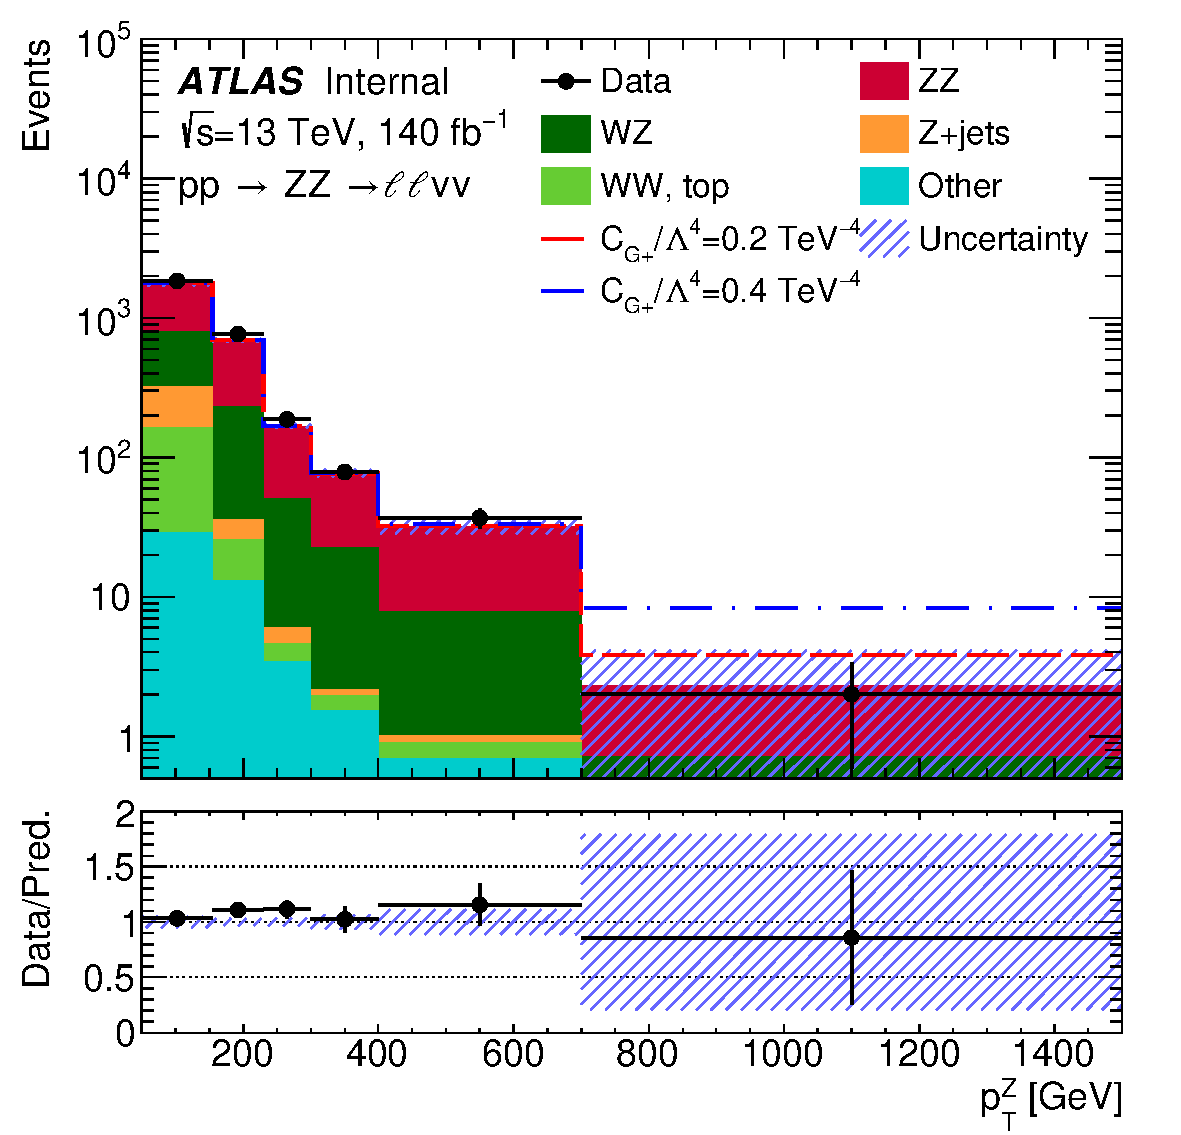
\includegraphics[width=0.6\linewidth]{figures/ch5-llvv/aTGC-aQGC/ptll_atgc.pdf}
    \caption{Distribution of the transverse momentum of the dilepton system, $p_\text{T}^{Z}$, including data and SM predictions.
    The dashed band represents the total systematic uncertainty in the SM prediction. The expected effects of an aTGC induced by the operator $O_{G+}$, for two representative values of the Wilson coefficient, are also shown.}
    \label{fig:ptll-aTGC}
\end{figure}

Limits on aTGC parameters are derived using two complementary frameworks: the vertex-function (VF) formalism~\cite{Baur2000,Biekotter2021} and the Standard Model Effective Field Theory (SMEFT)~\cite{Degrande:2013,Degrande2014,Ellis2023}. 

The most general anomalous $ZZV$ ($V=Z,\gamma$) vertex function for on-shell $Z$ bosons is given by~\cite{Hagiwara:1986vm}:
\begin{equation}
g_{ZZV}\Gamma_{ZZV}^{\alpha\beta\mu}
= e\frac{P^2-m_V^2}{m_Z^2}
\left[
if_4^V(P^{\alpha}g^{\mu\beta}+P^{\beta}g^{\mu\alpha})
+ if_5^V\epsilon^{\mu\alpha\beta\rho}(q_1-q_2)_\rho
\right],
\label{eqn:vtx_func}
\end{equation}
where $P$, $q_1$, and $q_2$ denote the momenta of the $V$ boson and the two on-shell $Z$ bosons, respectively. The anomalous couplings $f_4^V$ and $f_5^V$ correspond to CP-violating and CP-conserving interactions.

In the SMEFT framework, the Lagrangian is extended by dimension-eight operators:
\begin{equation}
\mathcal{L}_\text{SMEFT}
= \mathcal{L}_\text{SM}
+ \sum_i \frac{C_i}{\Lambda^4}\mathcal{O}_i^{(8)},
\label{eqn:eft}
\end{equation}
where $\mathcal{O}_i^{(8)}$ are dimension-eight operators and $C_i$ their Wilson coefficients. This analysis includes the operators 
$\mathcal{O}_{G+}$, $\mathcal{O}_{G-}$, $\mathcal{O}_{\widetilde{B}W}$, 
$\mathcal{O}_{BB}$, $\mathcal{O}_{BW}$, and $\mathcal{O}_{WW}$ with corresponding coefficients $C_i/\Lambda^4$~\cite{Degrande2014,Ellis2023}. 
The new-physics scale is fixed to $\Lambda = 1$~TeV.

The 95\% confidence level (CL) intervals for the VF parameters $f_4^{\gamma/Z}$ (CP-violating) and $f_5^{\gamma/Z}$ (CP-conserving), as well as for the SMEFT higher-dimensional operator coefficients, are presented in Table~\ref{tab:atgc_limits}. The results from the VF framework improve upon the previous ATLAS $ZZ \to \ell\ell\nu\nu$ measurement by approximately a factor of 1.7. The limits of the SMEFT coefficients are derived for the first time in this channel.

\begin{table}[htbp]
\centering
\scriptsize
\renewcommand{\arraystretch}{1.5}
\begin{tabular}{lccc}
\hline
\textbf{Model} & \textbf{Coefficient} & \textbf{Expected} & \textbf{Observed} \\
\hline
VF & $f_{4}^{\gamma}$ & $[-7.7,\ 7.7] \times 10^{-4}$ & $[-6.4,\ 6.4] \times 10^{-4}$ \\
VF & $f_{4}^{Z}$      & $[-6.8,\ 6.8] \times 10^{-4}$ & $[-5.7,\ 5.7] \times 10^{-4}$ \\
VF & $f_{5}^{\gamma}$ & $[-7.8,\ 7.7] \times 10^{-4}$ & $[-6.4,\ 6.5] \times 10^{-4}$ \\
VF & $f_{5}^{Z}$      & $[-6.9,\ 6.9] \times 10^{-4}$ & $[-5.8,\ 5.8] \times 10^{-4}$ \\
\hline
SMEFT &  $C_{G+}/\Lambda^4$         & $[-0.36,\ 0.36]$ & $[-0.29,\ 0.30]$ \\
SMEFT &  $C_{G-}/\Lambda^4$         & $[-1.1,\ 1.2]$   & $[-0.95,\ 0.95]$ \\
SMEFT & $C_{\tilde{B}W}/\Lambda^4$ & $[-1.3,\ 1.3]$   & $[-1.1,\ 1.1]$ \\
SMEFT &  $C_{BB}/\Lambda^4$         & $[-1.6,\ 1.6]$   & $[-1.3,\ 1.3]$ \\
SMEFT &  $C_{BW}/\Lambda^4$         & $[-2.9,\ 2.9]$   & $[-2.4,\ 2.4]$ \\
SMEFT & $C_{WW}/\Lambda^4$         & $[-2.4,\ 2.4]$   & $[-2.0,\ 2.0]$ \\
\hline
\end{tabular}
\caption{\rm Expected and observed 95\% CL intervals for the parameters of the VF and SMEFT formalisms derived from inclusive $ZZ$ production, obtained without applying any unitarization procedure. The limits are derived by varying one parameter at a time while setting all other aTGC parameters to zero.}
\label{tab:atgc_limits}
\end{table}







%\section{Electroweak $\text{ZZ}jj$ Production and Search for aQGCs}
%\label{sec:llvvjj}

\subsection{Constraints on Anomalous Quartic Gauge Couplings}
\label{subsec:aqgc_limits}

The measurement of $\text{ZZ}jj$ production is sensitive to the VBS processes, which offer a unique probe of quartic electroweak gauge boson interactions. In the context of the SMEFT framework, such effects are parameterised by extending the SM Lagrangian with higher-dimensional operators as follows: 
\begin{equation}
\mathcal{L}_\text{SMEFT} = \mathcal{L}_\text{SM} + \sum_i \frac{f_{\text{T}i}}{\Lambda^4} \mathcal{O}_{\text{T}i}^{(8)}.
\label{eqn:eft}
\end{equation}
Dimension-8 operators are considered here, as they directly contribute to quartic gauge couplings, which do not arise at lower dimensions~\cite{Eboli2016}.

As in Equation~\eqref{eqn:eft}, the SMEFT Lagrangian includes dimension-eight operators $\mathcal{O}_{\text{T}i}$, each associated with a Wilson coefficient $f_{\text{T}i}/ \Lambda^4$, where $i = 0, 1, \ldots, 9$, to distinguish them from the $C_i$ coefficients used for aTGCs in Section~\ref{sec:aTGC}.

%%%%%%%%%%%%%
$\text{ZZ}jj$ production provides direct sensitivity to the $\text{ZZWW}$ and $\text{ZZZZ}$ quartic vertices. In the SM, the cross-section contribution from these vertices is small. However, physics beyond the SM (BSM) could manifest as Anomalous Quartic Gauge Couplings (aQGCs), leading to a significant enhancement of the cross-section at high energy scales.

The aQGCs are parameterised using the Standard Model Effective Field Theory (SMEFT) framework. This analysis considers dimension-8 operators, specifically the transversal operators $\text{T}0$ through $\text{T}9$, which induce quartic couplings without modifying triple gauge couplings.

The most sensitive observable for detecting aQGCs is the transverse mass of the $\text{ZZ}$ system (see the distribution in Figure~\ref{fig:mTZZ-aQGC}), defined as:
\begin{equation}
    m_{\text{T}}^{\text{ZZ}} = \sqrt{ \left( \sqrt{m_{\text{Z}}^2 + (p_{\text{T}}^{\ell\ell})^2} + \sqrt{m_{\text{Z}}^2 + (E_{\text{T}}^{\text{miss}})^2} \right)^2 - \left| \vec{p}_{\text{T}}^{\ell\ell} + \vec{E}_{\text{T}}^{\text{miss}} \right|^2 }.
\end{equation}
The presence of aQGCs would appear as an excess of events in the high-$m_{\text{T}}^{\text{ZZ}}$ tail.

\begin{figure}
    \centering
    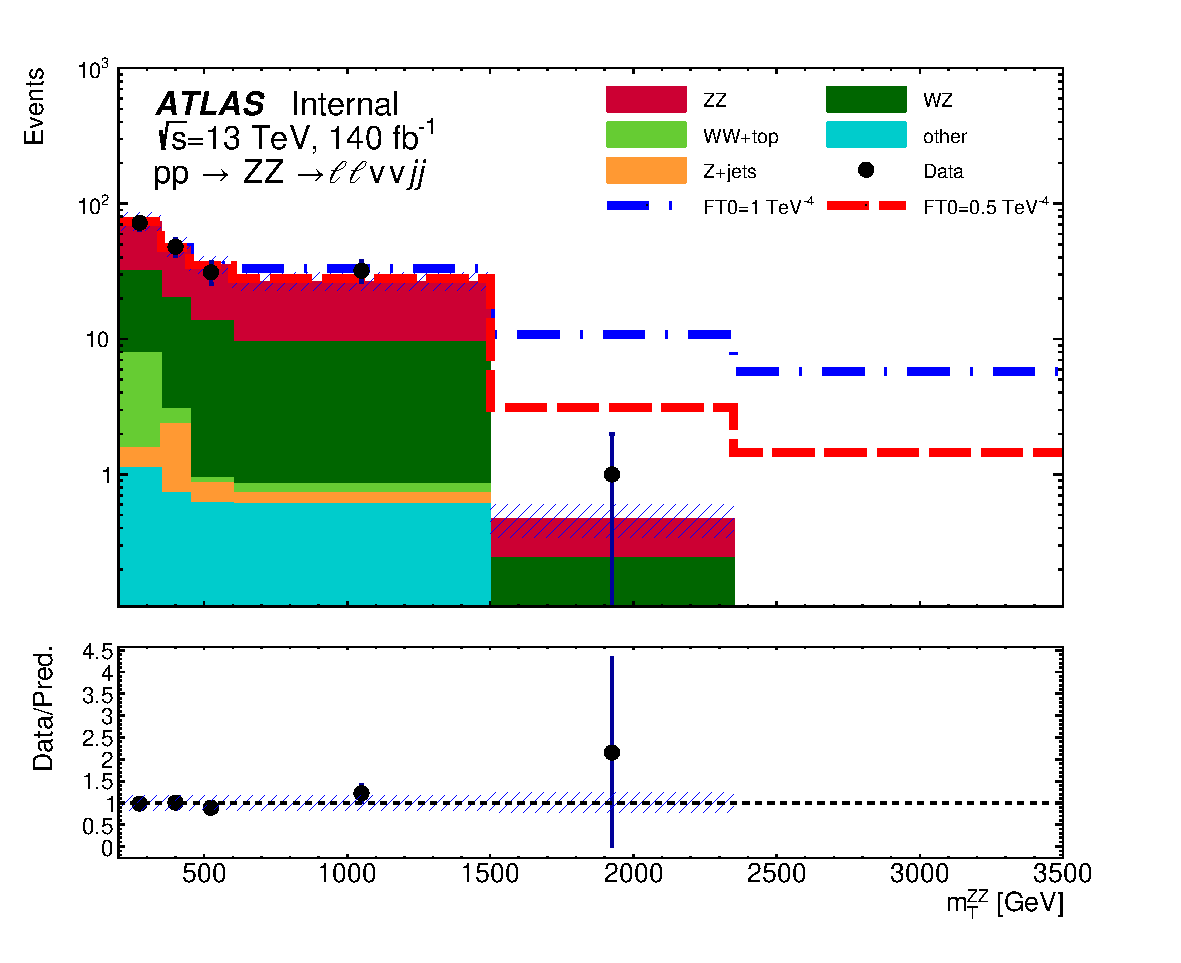
\includegraphics[width=0.6\linewidth]{figures/ch5-llvv/aTGC-aQGC/FT0_mTZZ_events.pdf}
    \caption{Comparison between data and MC predictions for the transverse mass of the $\text{ZZ}$ system, $m_{\text{T}}^{\text{ZZ}}$, at detector level. Predictions in the SMEFT framework for the $f_{\text{T}0}$ operator and two values of the Wilson coefficient are also shown.}
    \label{fig:mTZZ-aQGC}
\end{figure}

%\subsubsection{Limits on Wilson Coefficients}
The reconstructed transverse mass of the $\text{ZZ}$ system, $m_{\text{T}}^{\text{ZZ}}$, shown in Figure~\ref{fig:mTZZ-aQGC}, is used to extract limits on dimension-8 SMEFT operators. A binned likelihood fit to the $m_{\text{T}}^{\text{ZZ}}$ spectrum in the $\text{ZZ}jj$ signal region (SR) is performed to derive 95\% confidence level (CL) intervals for the Wilson coefficients $f_{\text{T}i}/\Lambda^4$ ($i = 0$--$9$). Systematic uncertainties are incorporated as nuisance parameters in the fit. The resulting limits are summarised in Table~\ref{tab:combined_run2_ZZjj_eft_intervals}, where each coefficient is varied individually while all others are set to zero.

To ensure the validity of the SMEFT expansion, unitarity-preserving cut-offs are applied to the BSM contributions by restricting $m_{\text{ZZ}} < E_{\text{c}}$, where $E_{\text{c}}$ denotes the energy cut-off scale.

\begin{table}[!htbp]
\centering
\scriptsize
\renewcommand{\arraystretch}{1.5}
\begin{tabular}{l c c c c c c}
\hline
\textbf{Wilson Coefficient} & 
\multicolumn{2}{c}{\textbf{No cut-off}} & 
\multicolumn{2}{c}{\textbf{$E_{\text{c}} = 1~\text{TeV}$}} & 
\multicolumn{2}{c}{\textbf{$E_{\text{c}} = 1.5~\text{TeV}$}} \\
\cline{2-7}
& \textbf{Expected} & \textbf{Observed} & 
  \textbf{Expected} & \textbf{Observed} & 
  \textbf{Expected} & \textbf{Observed} \\
\hline
$f_{\text{T}0}/\Lambda^4$ & $[-0.42,\ 0.40]$ & $[-0.50,\ 0.49]$ & $[-3.9,\ 3.8]$ & $[-4.9,\ 4.9]$ & $[-2.8,\ 2.6]$ & $[-4.0,\ 3.4]$ \\
$f_{\text{T}1}/\Lambda^4$ & $[-0.46,\ 0.46]$ & $[-0.56,\ 0.56]$ & $[-3.7,\ 3.6]$ & $[-4.6,\ 4.6]$ & $[-2.9,\ 2.8]$ & $[-3.8,\ 3.8]$ \\
$f_{\text{T}2}/\Lambda^4$ & $[-0.95,\ 0.93]$ & $[-1.1,\ 1.1]$ & $[-7.7,\ 7.6]$ & $[-9.8,\ 9.7]$ & $[-5.9,\ 5.6]$ & $[-7.7,\ 7.4]$ \\
$f_{\text{T}3}/\Lambda^4$ & $[-1.3,\ 1.3]$ & $[-1.6,\ 1.6]$ & $[-9.9,\ 9.9]$ & $[-13,\ 13]$ & $[-7.7,\ 7.4]$ & $[-10.0,\ 9.7]$ \\
$f_{\text{T}4}/\Lambda^4$ & $[-8.8,\ 8.5]$ & $[-11,\ 11]$ & $[-55,\ 54]$ & $[-69,\ 69]$ & $[-43,\ 41]$ & $[-56,\ 53]$ \\
$f_{\text{T}5}/\Lambda^4$ & $[-0.75,\ 0.71]$ & $[-0.89,\ 0.87]$ & $[-6.9,\ 6.7]$ & $[-8.7,\ 8.6]$ & $[-4.8,\ 4.4]$ & $[-6.2,\ 5.8]$ \\
$f_{\text{T}6}/\Lambda^4$ & $[-1.1,\ 1.1]$ & $[-1.4,\ 1.4]$ & $[-6.9,\ 6.9]$ & $[-8.9,\ 8.9]$ & $[-5.4,\ 5.3]$ & $[-7.1,\ 7.0]$ \\
$f_{\text{T}7}/\Lambda^4$ & $[-2.5,\ 2.4]$ & $[-3.0,\ 3.0]$ & $[-14,\ 14]$ & $[-18,\ 18]$ & $[-18,\ 18]$ & $[-22,\ 21]$ \\
$f_{\text{T}8}/\Lambda^4$ & $[-0.60,\ 0.60]$ & $[-0.74,\ 0.74]$ & $[-6.7,\ 6.7]$ & $[-8.7,\ 8.7]$ & $[-3.8,\ 3.8]$ & $[-4.9,\ 4.9]$ \\
$f_{\text{T}9}/\Lambda^4$ & $[-1.3,\ 1.3]$ & $[-1.6,\ 1.6]$ & $[-14,\ 14]$ & $[-18,\ 18]$ & $[-7.9,\ 7.9]$ & $[-10.0,\ 10.0]$ \\
\hline
\end{tabular}
\caption{\rm Expected and observed 95\% CL intervals for the dimension-8 Wilson coefficients in the 
$\text{ZZ}jj \to \ell\ell\nu\nu jj$ phase space, derived from a one-dimensional fit to the $m_{\text{T}}^{\text{ZZ}}$ spectrum. Results are shown for three EFT validity scenarios: without unitarisation, and with energy cut-offs at $1~\text{TeV}$ and $1.5~\text{TeV}$.}
\label{tab:combined_run2_ZZjj_eft_intervals}
\end{table}

The observed limits are consistent with zero for all operators. To further assess the validity of the EFT expansion, unitarity bounds are evaluated as a function of the energy cut-off scale $E_{\text{c}}$.

Figures~\ref{fig:fT0-fT1_zzjj_EFT} and~\ref{fig:fT2-fT9_zzjj_EFT} show the evolution of the limits on the Wilson coefficients $f_{\text{T}i}$ ($i = 0$--$9$) as a function of $E_{\text{c}}$. The unitarity bounds shown in these figures indicate the parameter values above which the SMEFT description becomes invalid due to violation of perturbative unitarity. They are computed following the prescription in Ref.~\cite{Almeida:2020ylr}, based on the energy scale at which the partonic scattering amplitude exceeds the unitarity limit.

Notably, the constraints obtained in this $\ell\ell\nu\nu jj$ analysis are significantly tighter than those from the fully leptonic $\text{ZZ} \to 4\ell jj$ channel, improving the sensitivity by more than a factor of two. This improvement is driven primarily by the larger branching ratio of the $\text{Z} \to \nu\nu$ decay compared to $\text{Z} \to \ell\ell$, which preserves statistics in the high-$m_{\text{T}}^{\text{ZZ}}$ tail where the aQGC sensitivity is highest.

\begin{figure}[htbp]
    \centering
    % Top Row: fT0 and fT1
    \subfloat[]{
        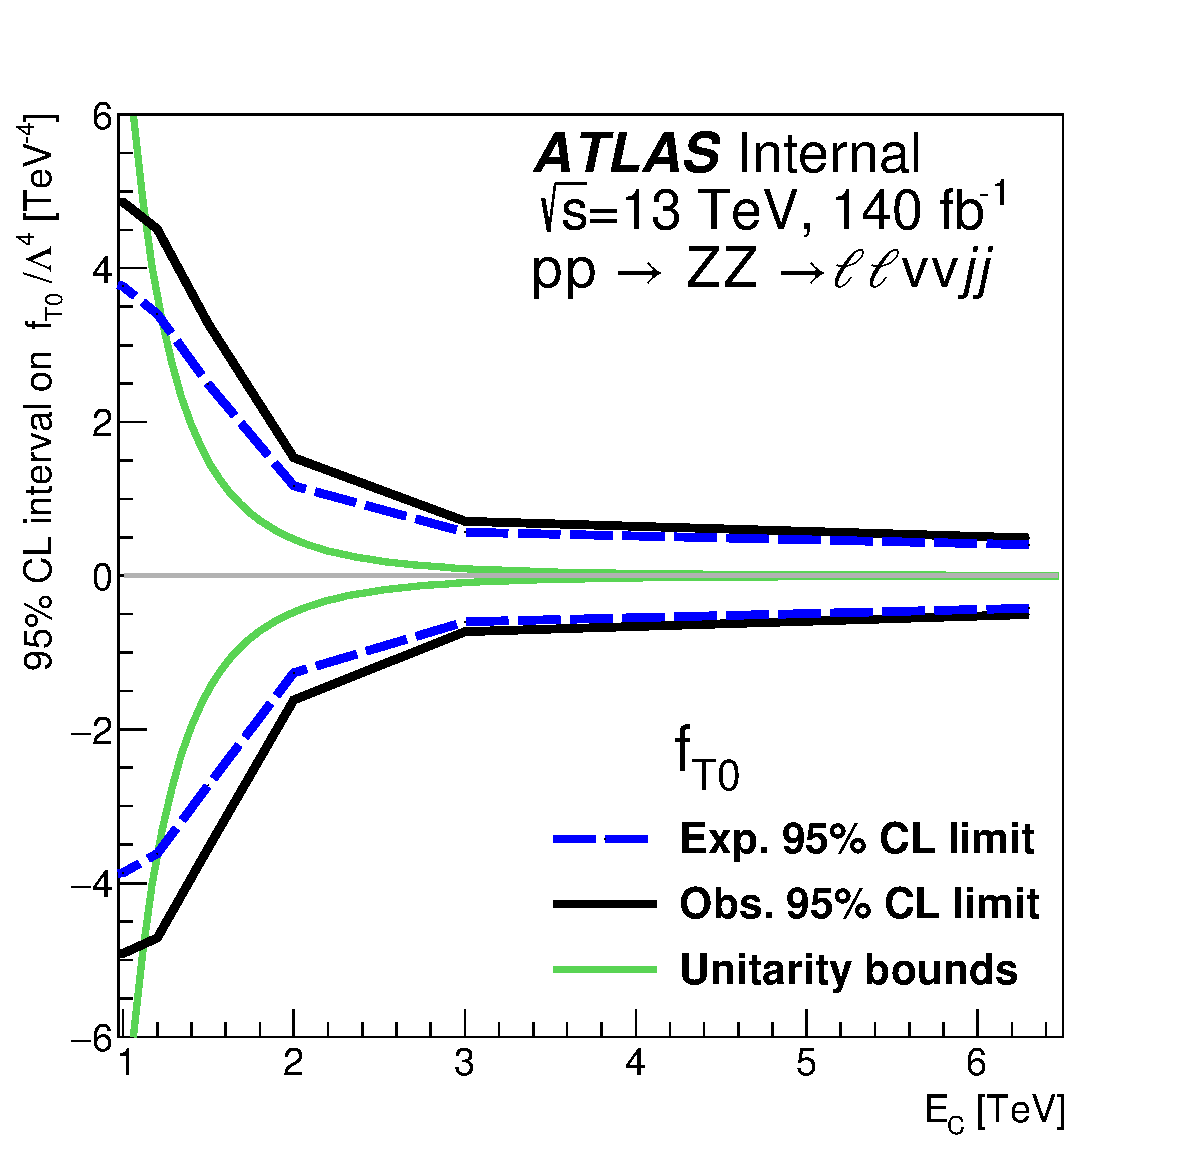
\includegraphics[width=0.45\linewidth]{figures/ch5-llvv/aTGC-aQGC/FT0.pdf}
        \label{fig:aqgc_fT0}
    }
    \hfill
    \subfloat[]{
        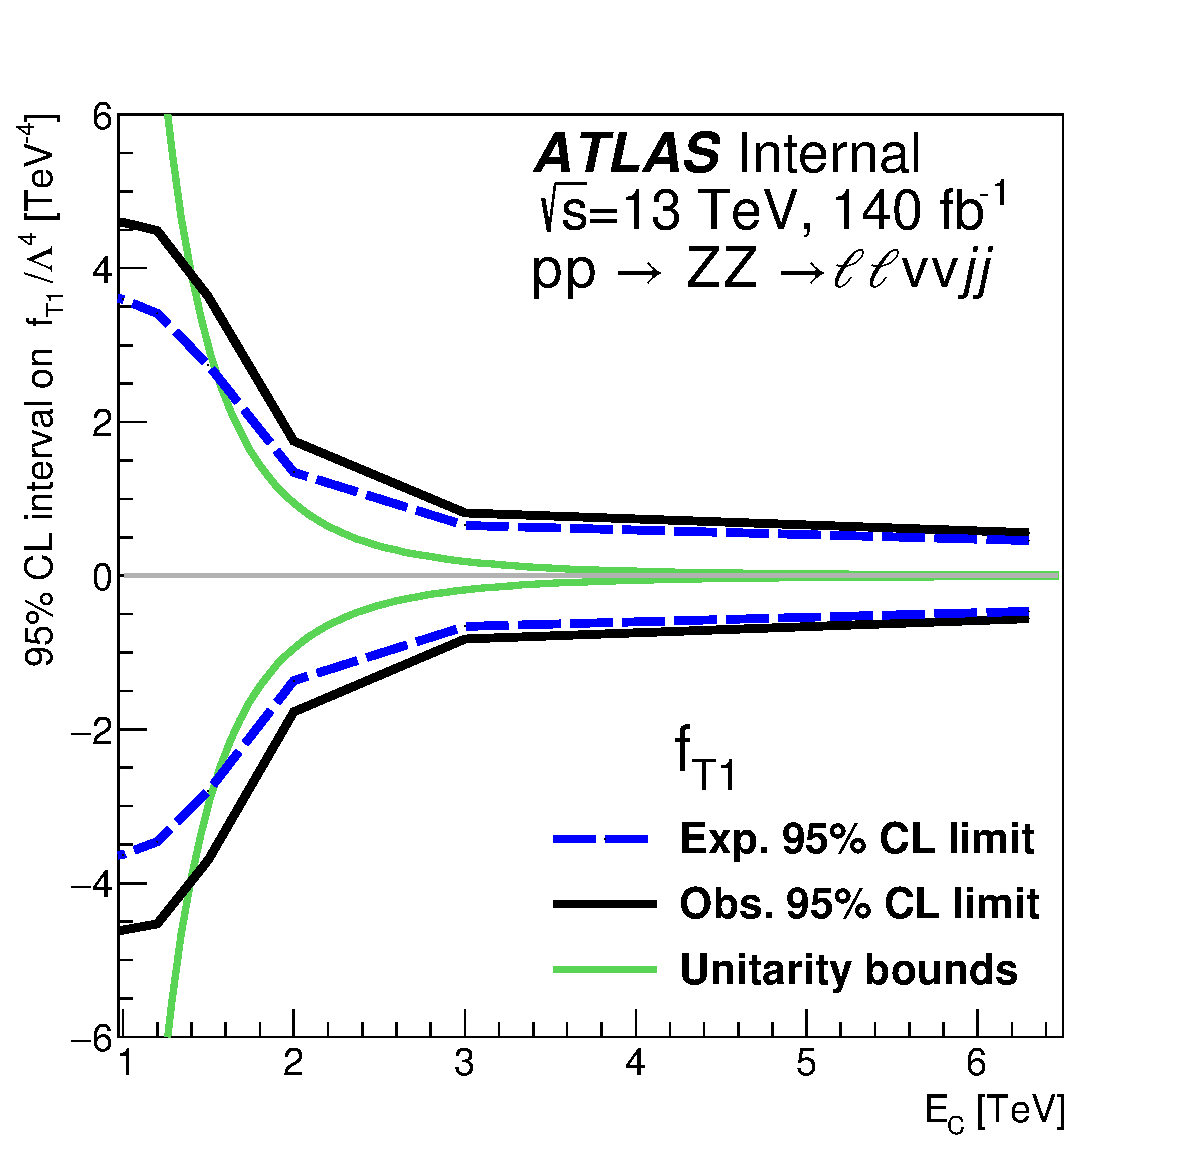
\includegraphics[width=0.45\linewidth]{figures/ch5-llvv/aTGC-aQGC/FT1.pdf}
        \label{fig:aqgc_fT1}
    }
    \\ % Line break for Bottom Row
    % Bottom Row: fT2 and fT3
    \subfloat[]{
        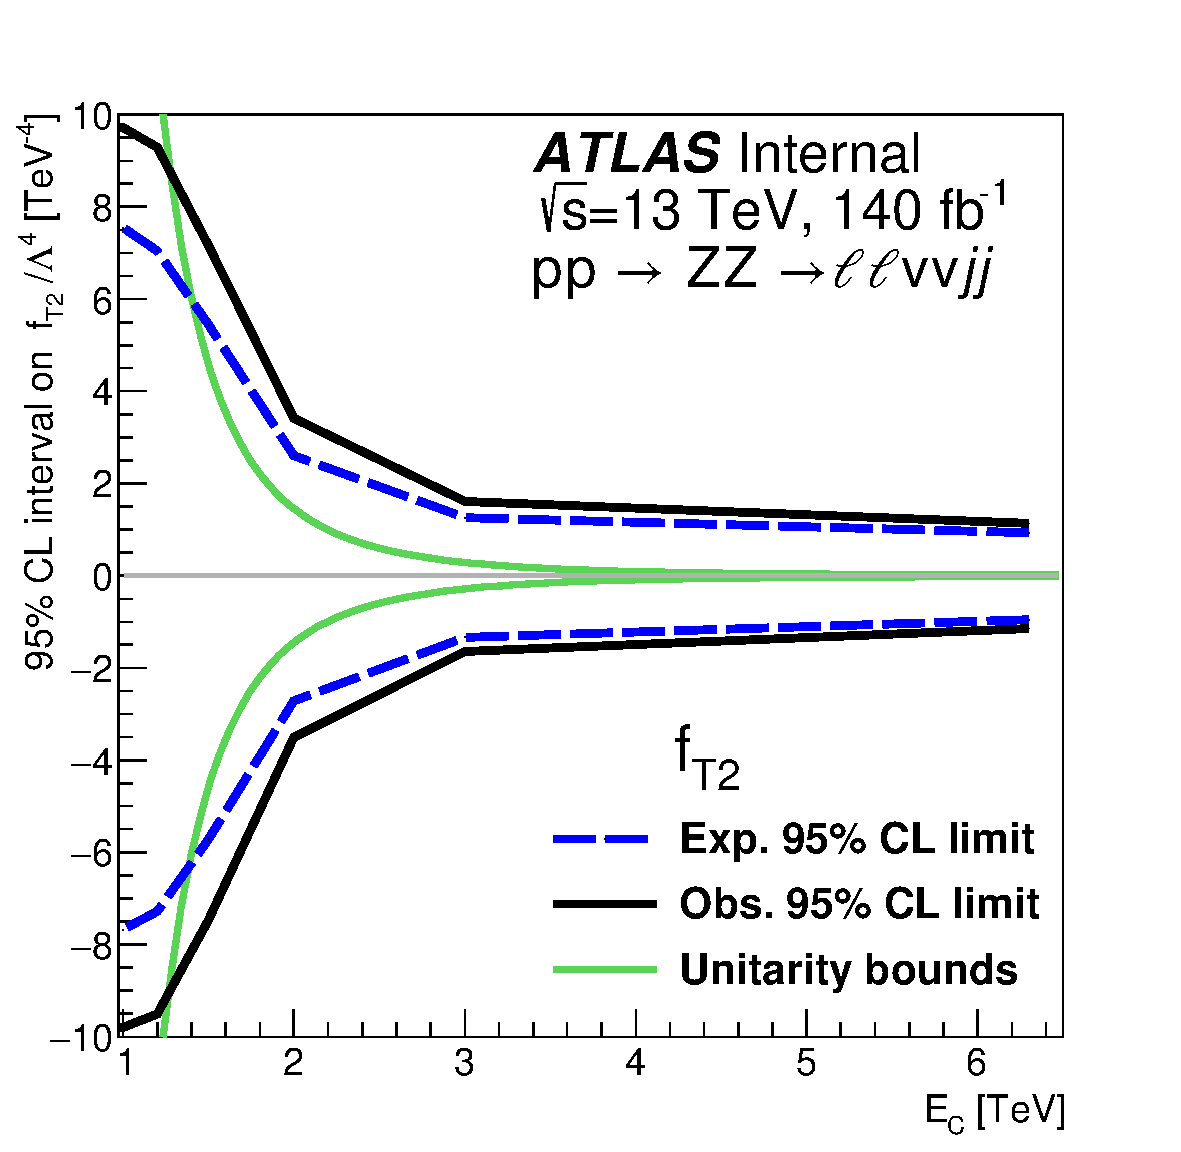
\includegraphics[width=0.45\linewidth]{figures/ch5-llvv/aTGC-aQGC/FT2.pdf}
        \label{fig:aqgc_fT2}
    }
    \hfill
    \subfloat[]{
        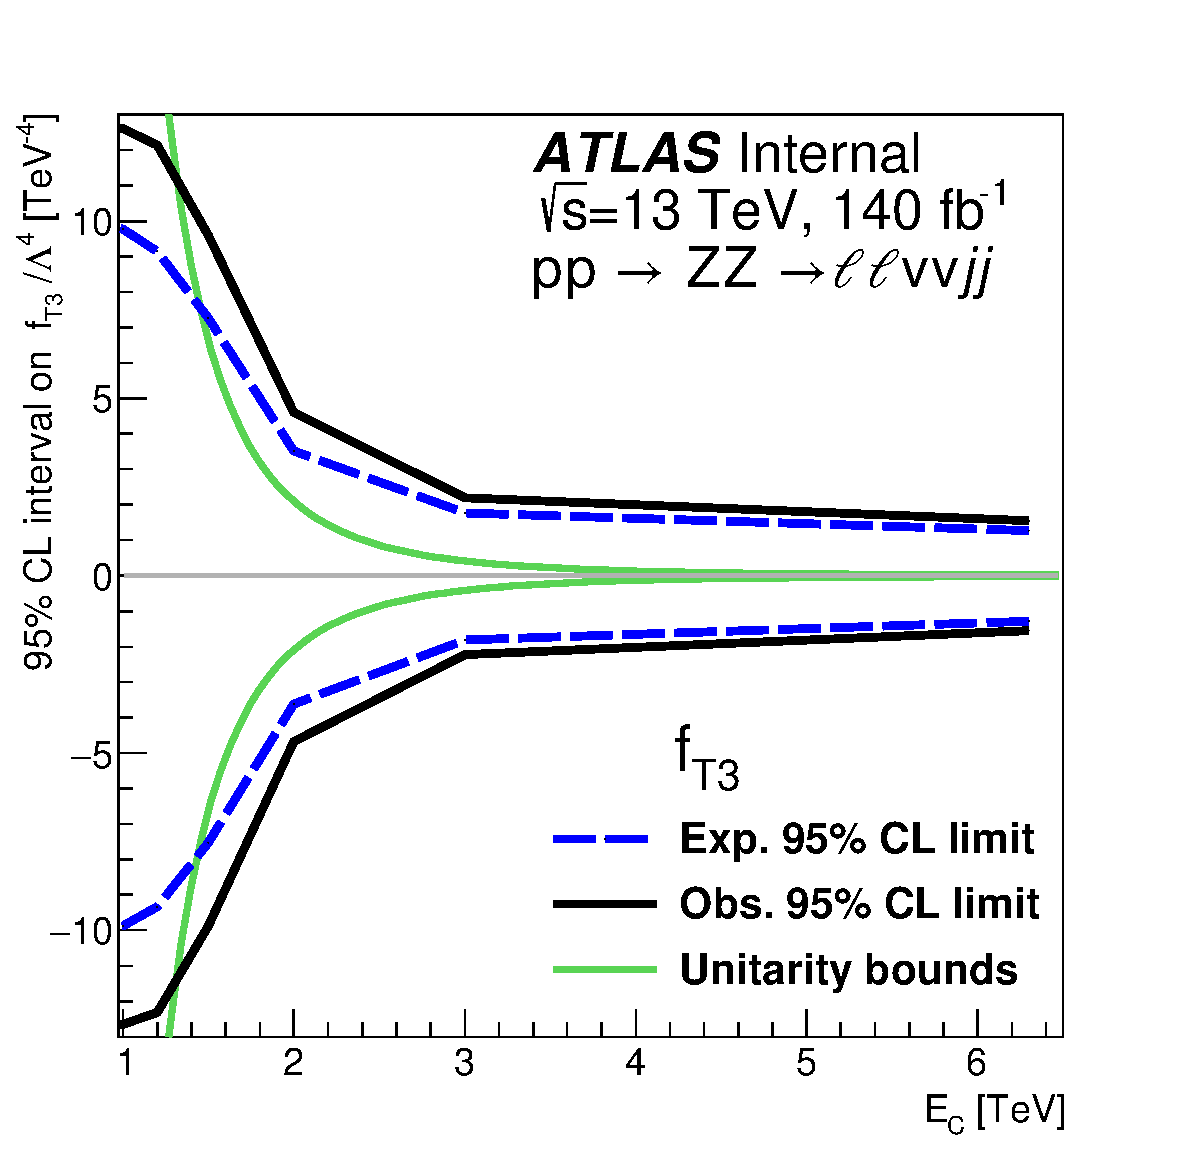
\includegraphics[width=0.45\linewidth]{figures/ch5-llvv/aTGC-aQGC/FT3.pdf}
        \label{fig:fT0-fT1_zzjj_EFT}
    }
    
    \caption{Expected and observed 95\% CL intervals for the Wilson coefficients (a) $f_{\text{T}0}$, (b) $f_{\text{T}1}$, (c) $f_{\text{T}2}$, and (d) $f_{\text{T}3}$ as a function of the EFT cut-off scale $E_{\text{c}}$. 
    The cut-off scale imposes a restriction such that the BSM amplitudes are set to zero when $m_{\text{ZZ}} > E_{\text{c}}$. 
    The dashed (solid) lines show the expected (observed) limits, and the solid green curve corresponds to the unitarity bounds.}
    \label{fig:aqgc_limits_fT0_fT3}
\end{figure}

\begin{figure}[!htbp]
    \centering
    \subfloat[]{
    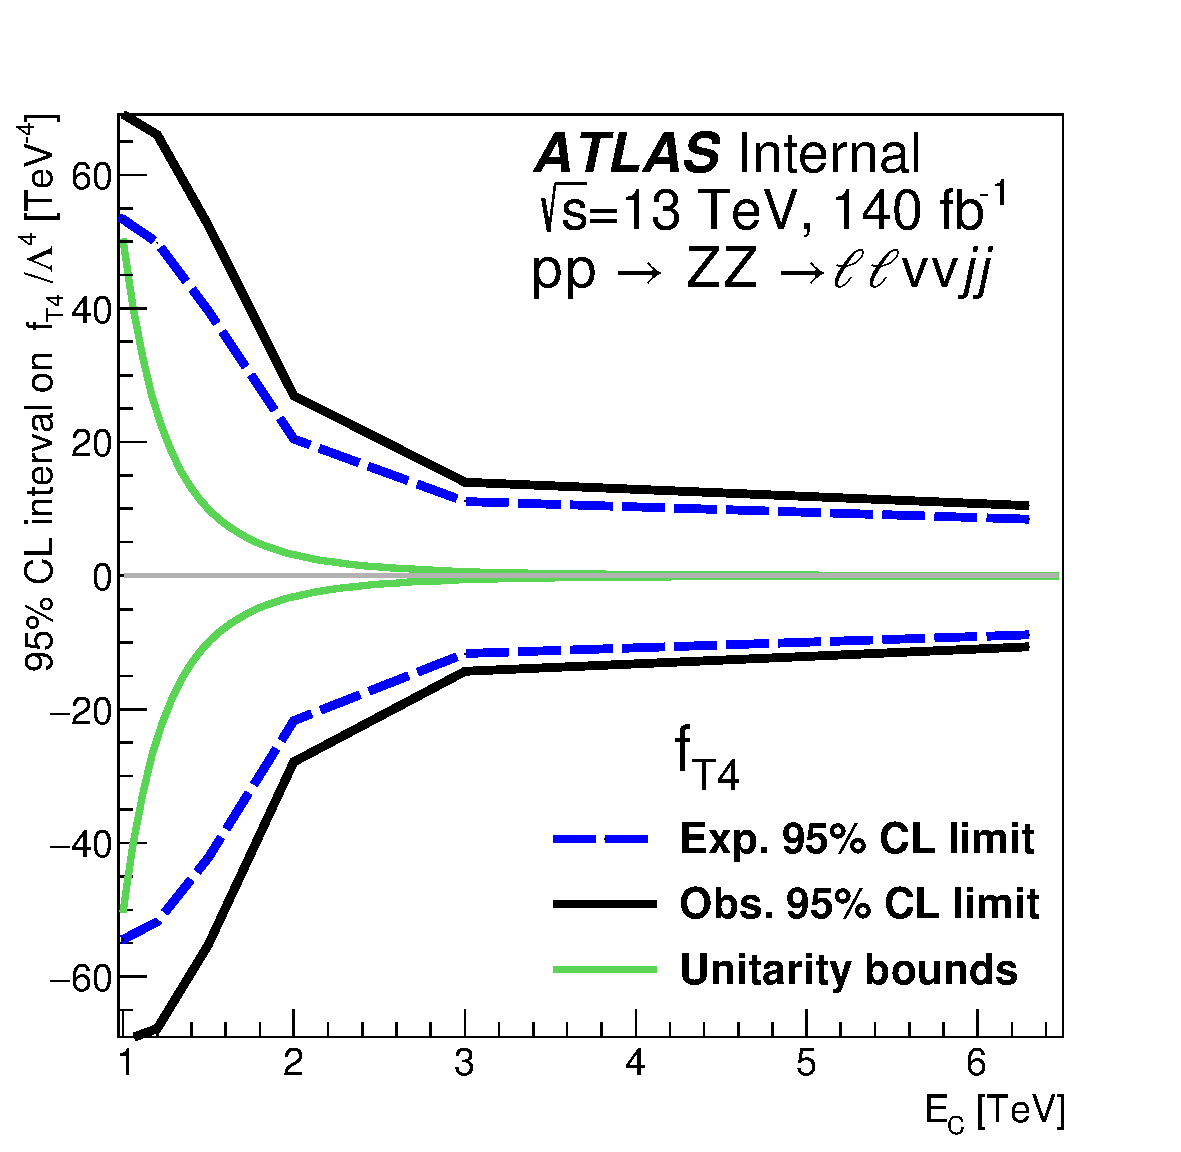
\includegraphics[width=0.45\linewidth]{figures/ch5-llvv/aTGC-aQGC/FT4.pdf}}
    \subfloat[]{
    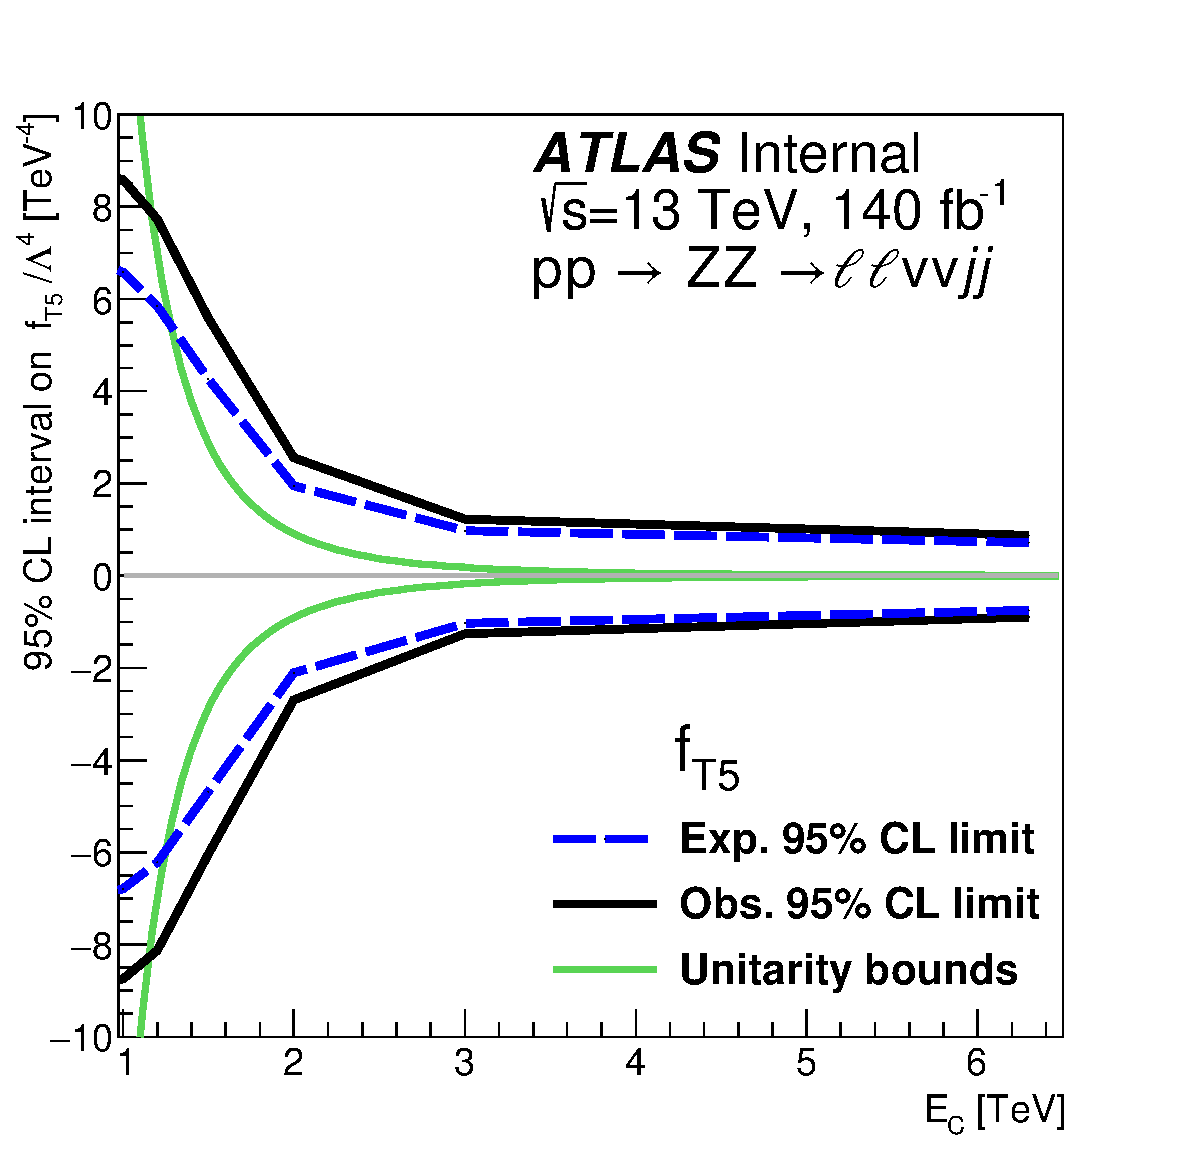
\includegraphics[width=0.45\linewidth]{figures/ch5-llvv/aTGC-aQGC/FT5.pdf}}
    \\
    \subfloat[]{
    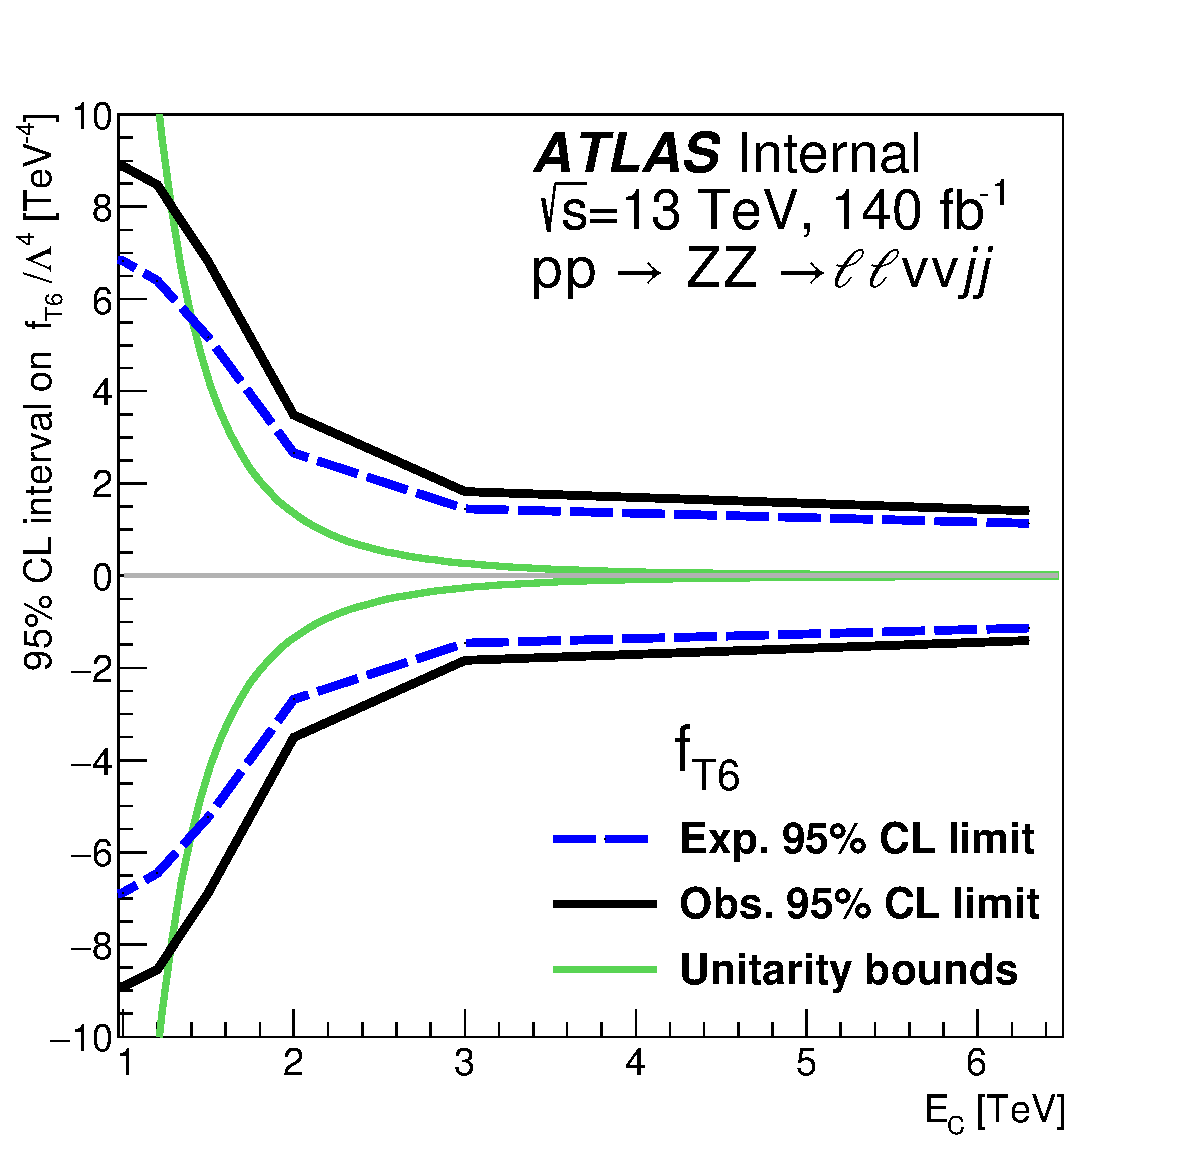
\includegraphics[width=0.45\linewidth]{figures/ch5-llvv/aTGC-aQGC/FT6.pdf}}
    \subfloat[]{
    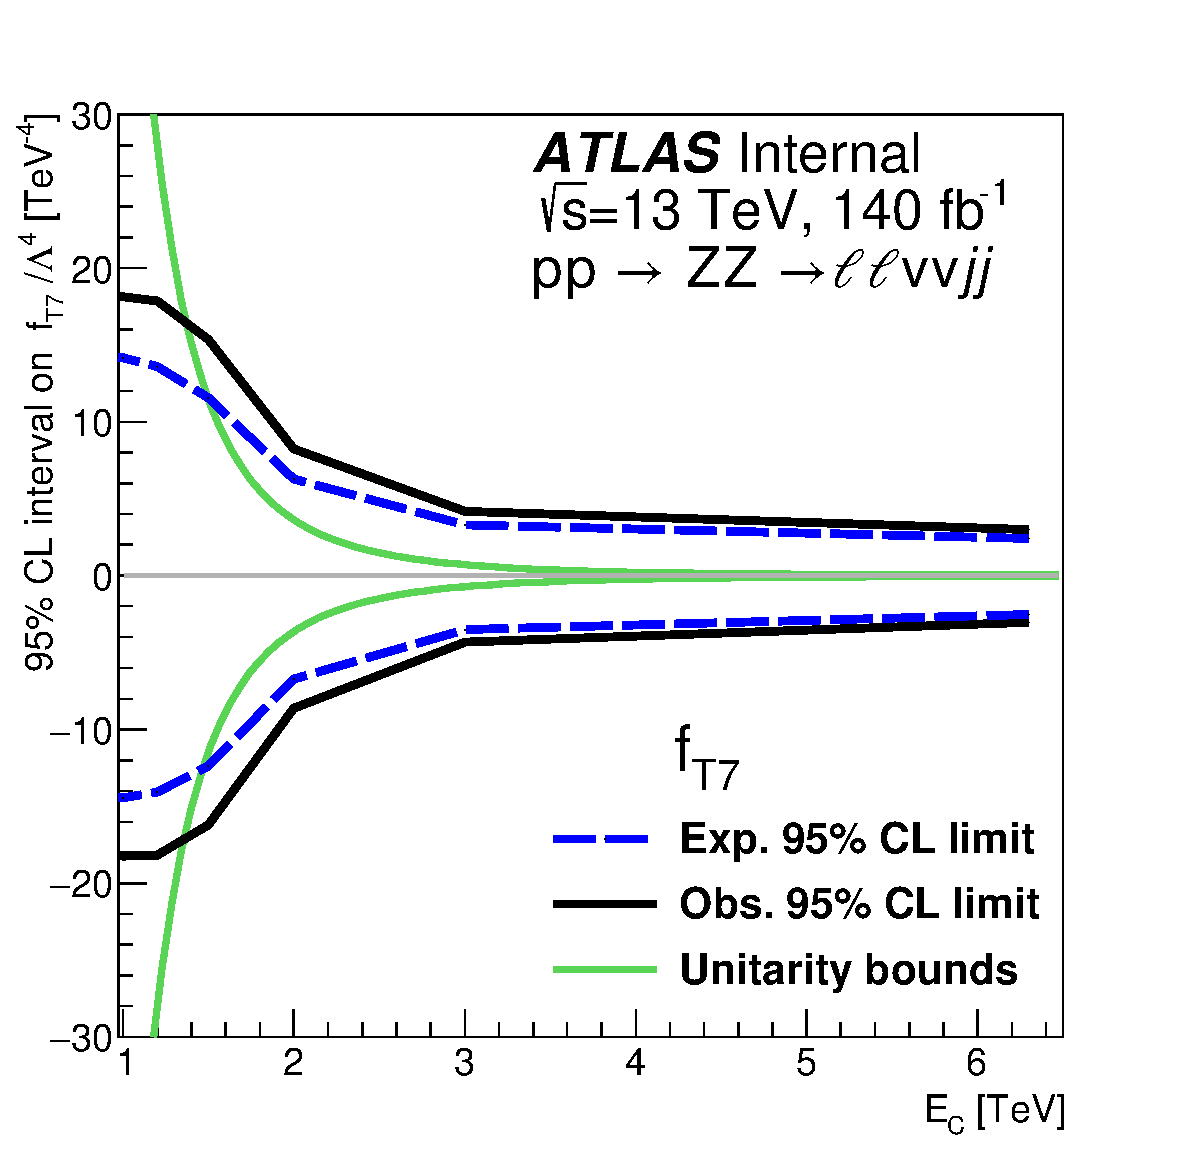
\includegraphics[width=0.45\linewidth]{figures/ch5-llvv/aTGC-aQGC/FT7.pdf}} 
    \\
    \subfloat[]{
    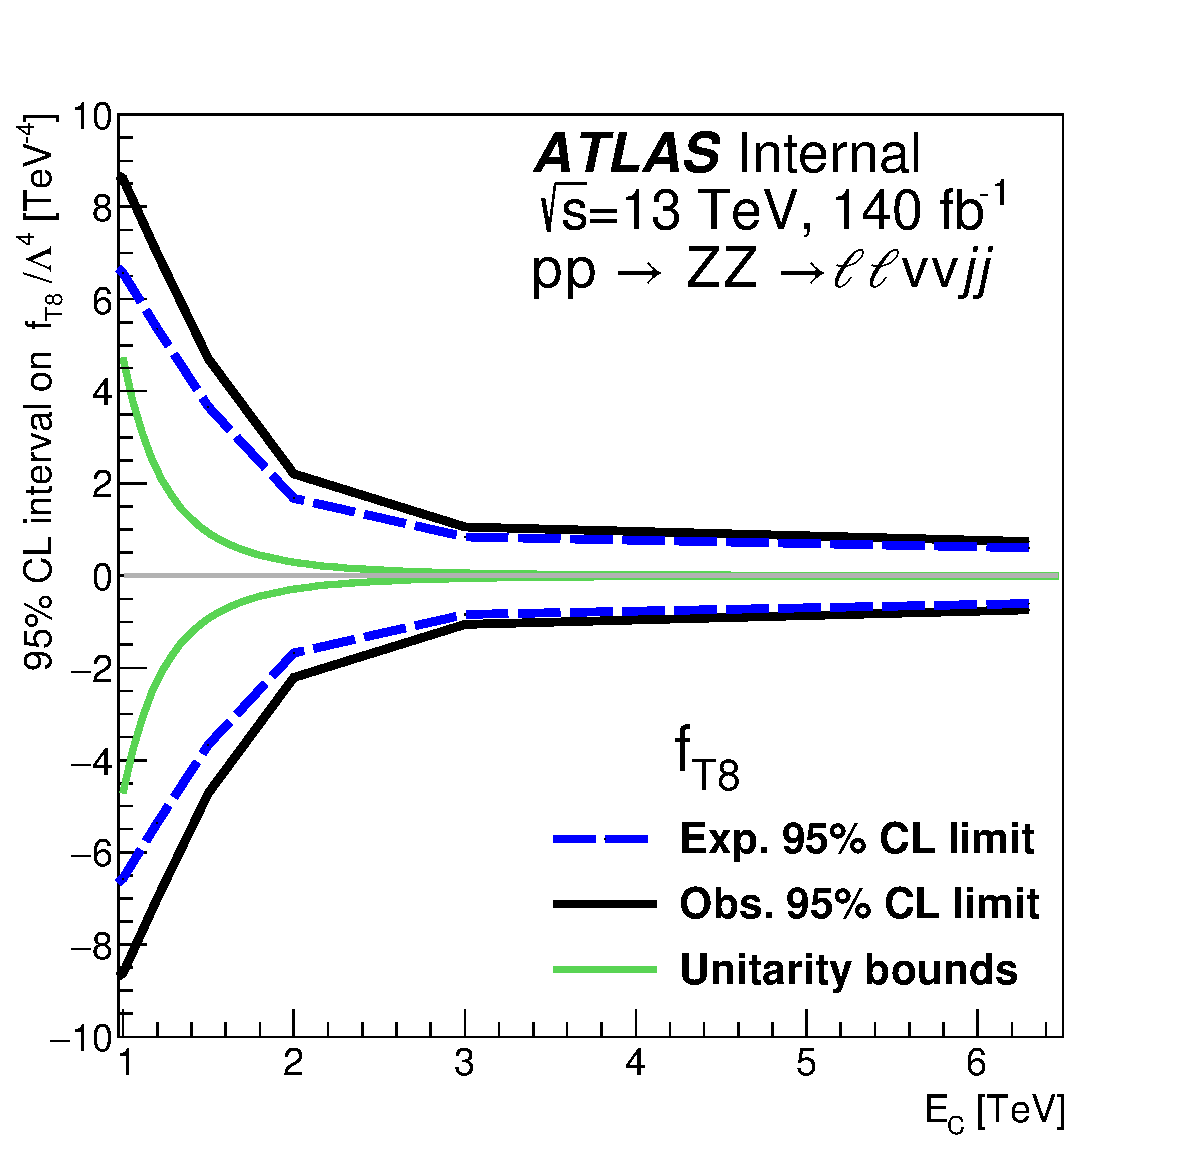
\includegraphics[width=0.45\linewidth]{figures/ch5-llvv/aTGC-aQGC/FT8.pdf}} 
    \subfloat[]{
    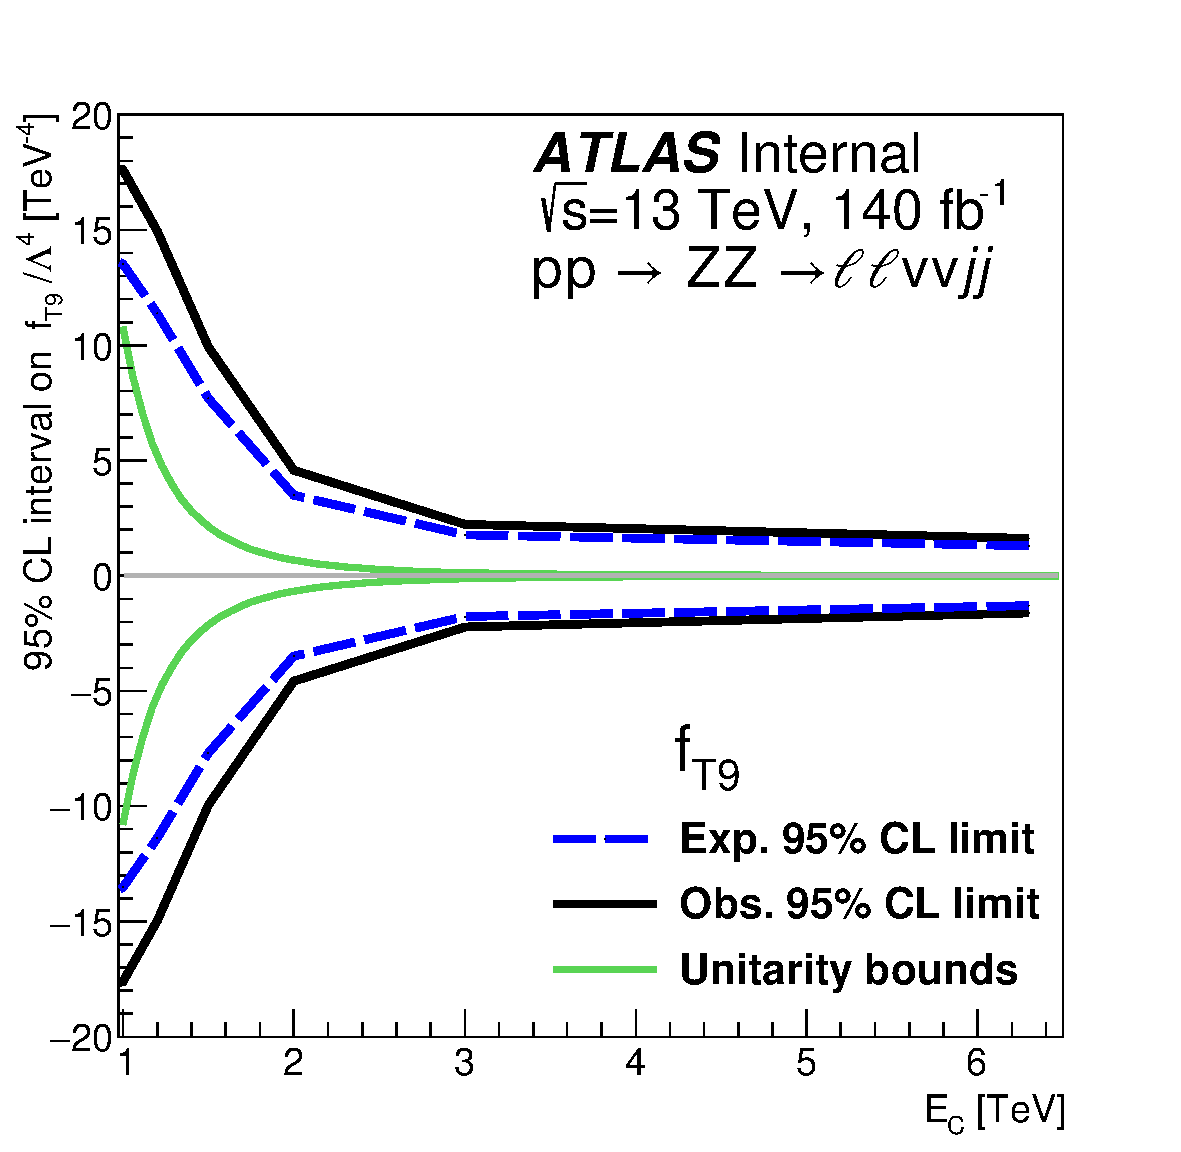
\includegraphics[width=0.45\linewidth]{figures/ch5-llvv/aTGC-aQGC/FT9.pdf}}
    \\
    \caption{The expected and observed 95\% CL for the $f_{\text{T}4}$ (a), $f_{\text{T}5}$ (b), $f_{\text{T}6}$ (c), $f_{\text{T}7}$ (d), $f_{\text{T}8}$ (e) and $f_{\text{T}9}$ (f) Wilson coefficients are derived as a function of the cut-off scale, $E_{\text{c}}$, which imposes a restriction such that the BSM amplitudes of interference and pure dimension-eight are set to zero when $m_{\text{ZZ}} > E_{\text{c}}$. 
These constraints are determined by performing a one-dimensional fit to the $m_{\text{T}}^{\text{ZZ}}$ distribution in the $\ell\ell\nu\nu jj$ signal region. 
The dashed (solid) lines show the expected (observed) 95\% CL limits, and the solid curve corresponds to the unitarity bounds~\cite{Almeida:2020ylr}.
 }
    \label{fig:fT2-fT9_zzjj_EFT}
\end{figure}


% \begin{figure}[htbp]
%     \centering
%     % Row 1
%     \subfloat[]{
%         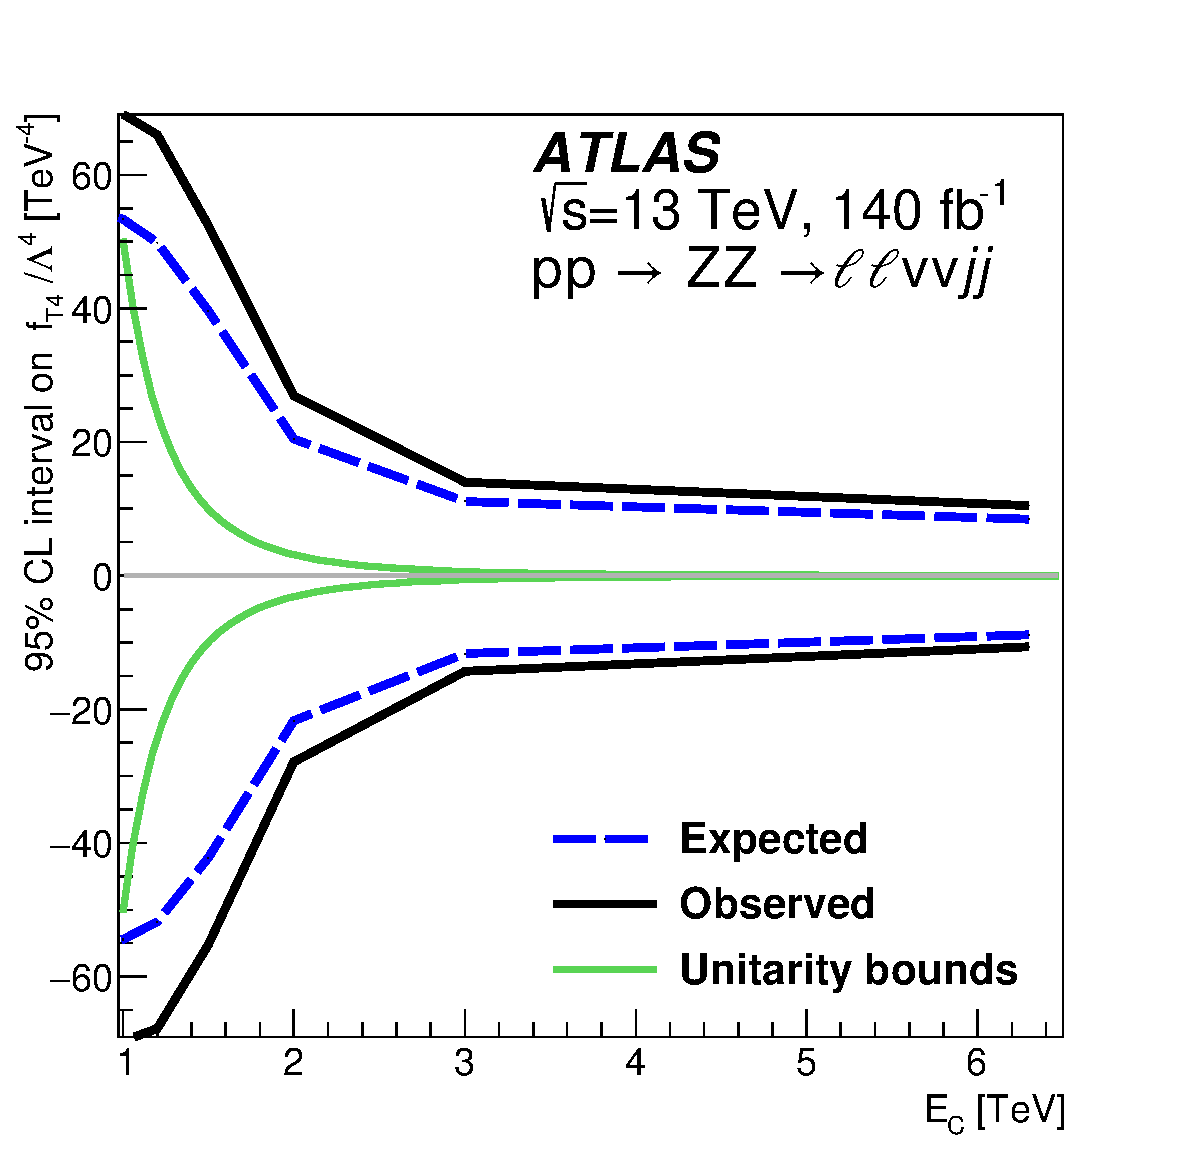
\includegraphics[width=0.32\textwidth]{figures/ch5-llvv/fig_aqgc_limit_fT4.pdf}
%         \label{fig:aqgc_fT4}
%     }
%     \hfill
%     \subfloat[]{
%         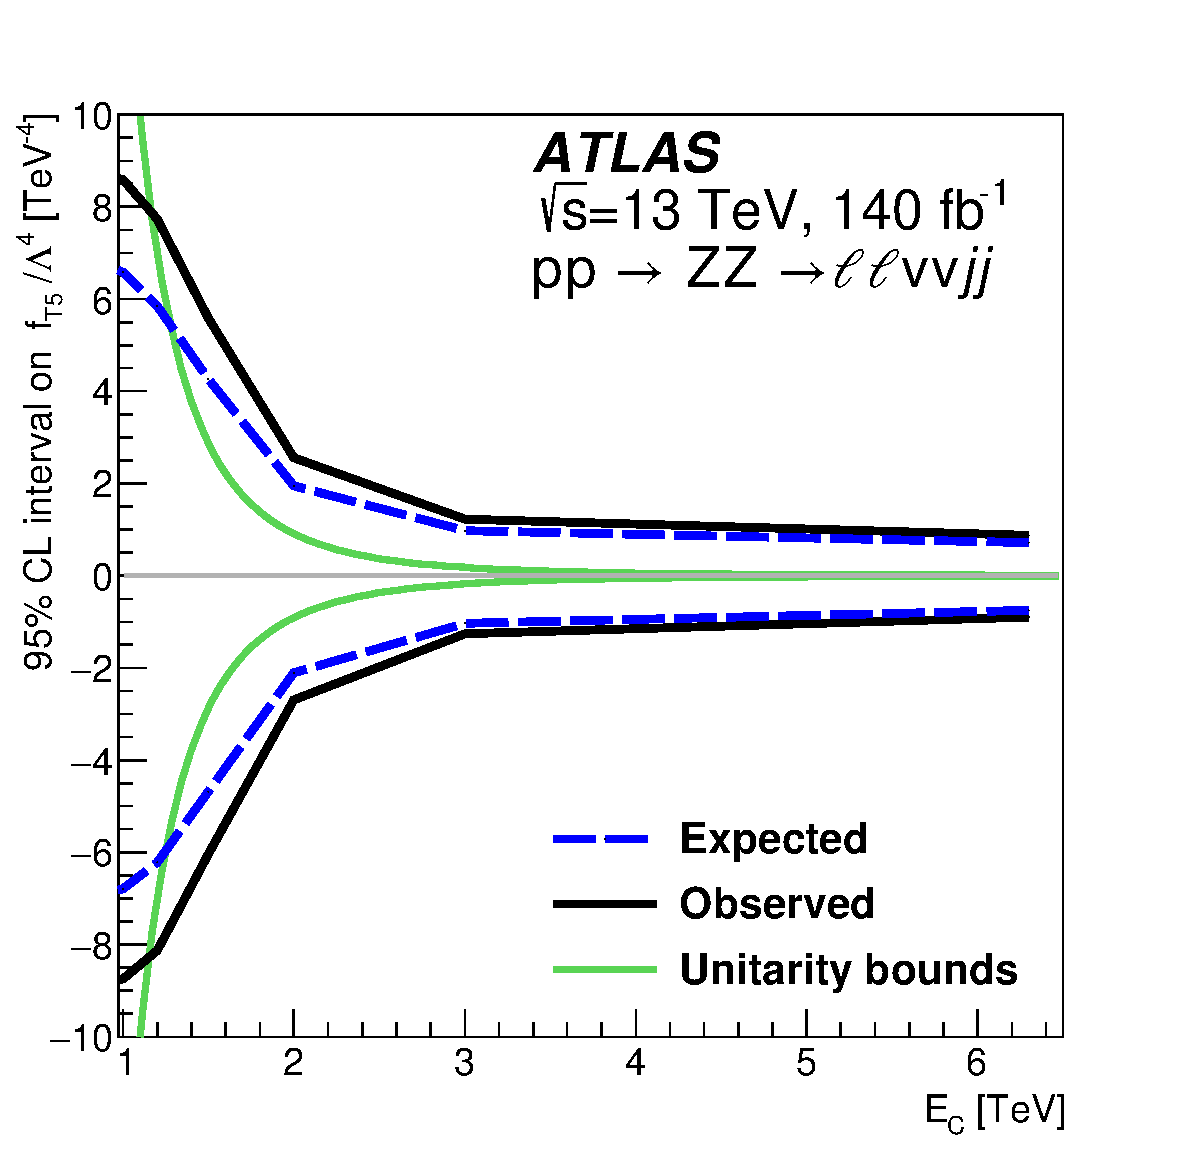
\includegraphics[width=0.32\textwidth]{figures/ch5-llvv/fig_aqgc_limit_fT5.pdf}
%         \label{fig:aqgc_fT5}
%     }
%     \hfill
%     \subfloat[]{
%         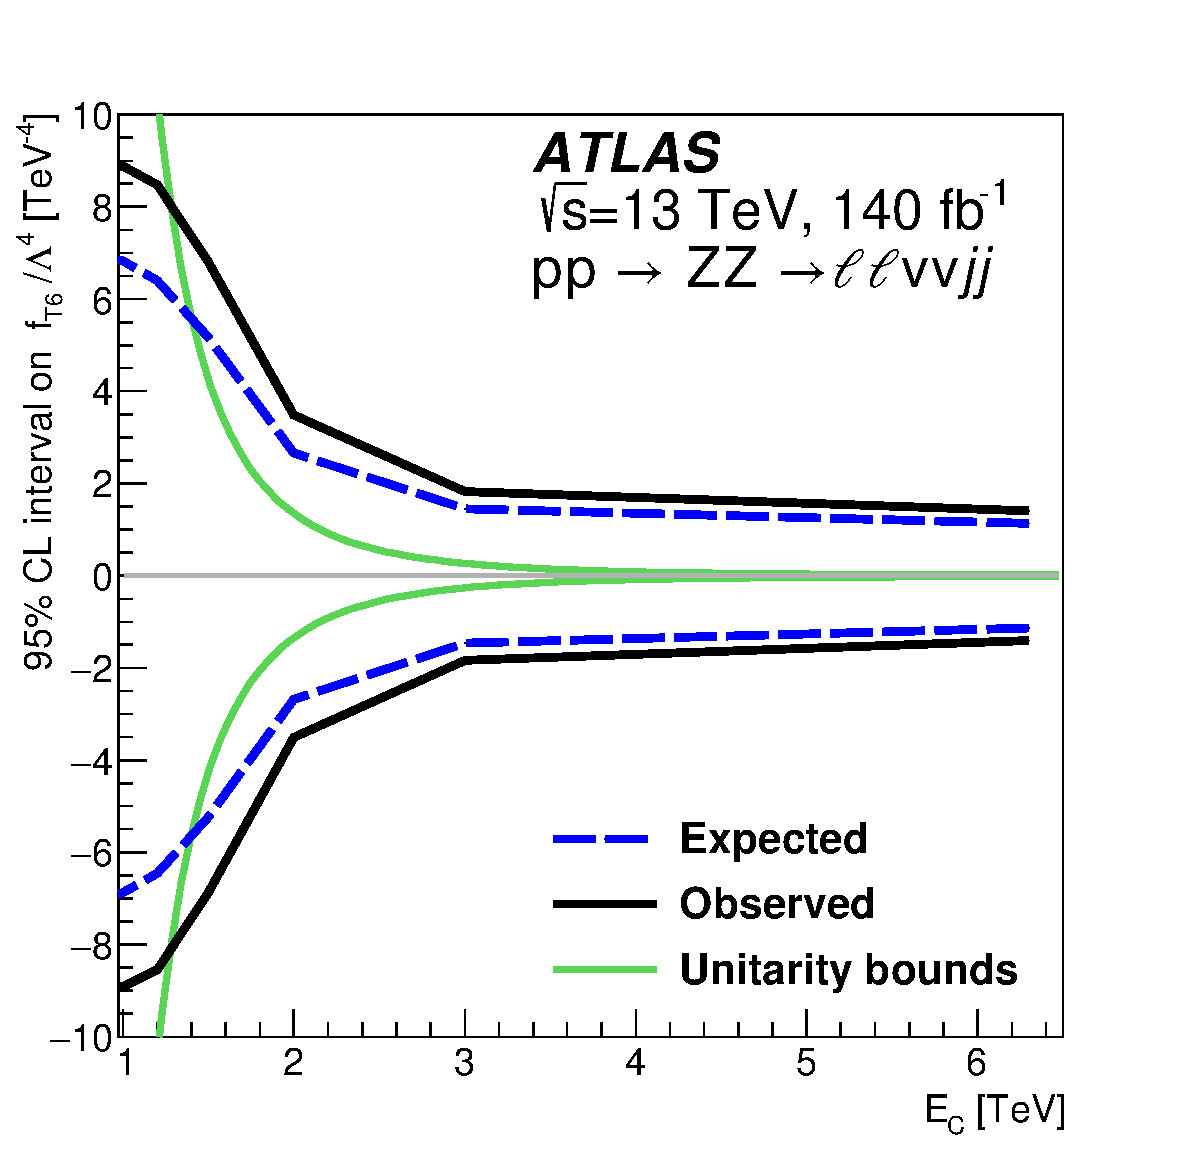
\includegraphics[width=0.32\textwidth]{figures/ch5-llvv/fig_aqgc_limit_fT6.pdf}
%         \label{fig:aqgc_fT6}
%     }
%     \\ % Line break
%     % Row 2
%     \subfloat[]{
%         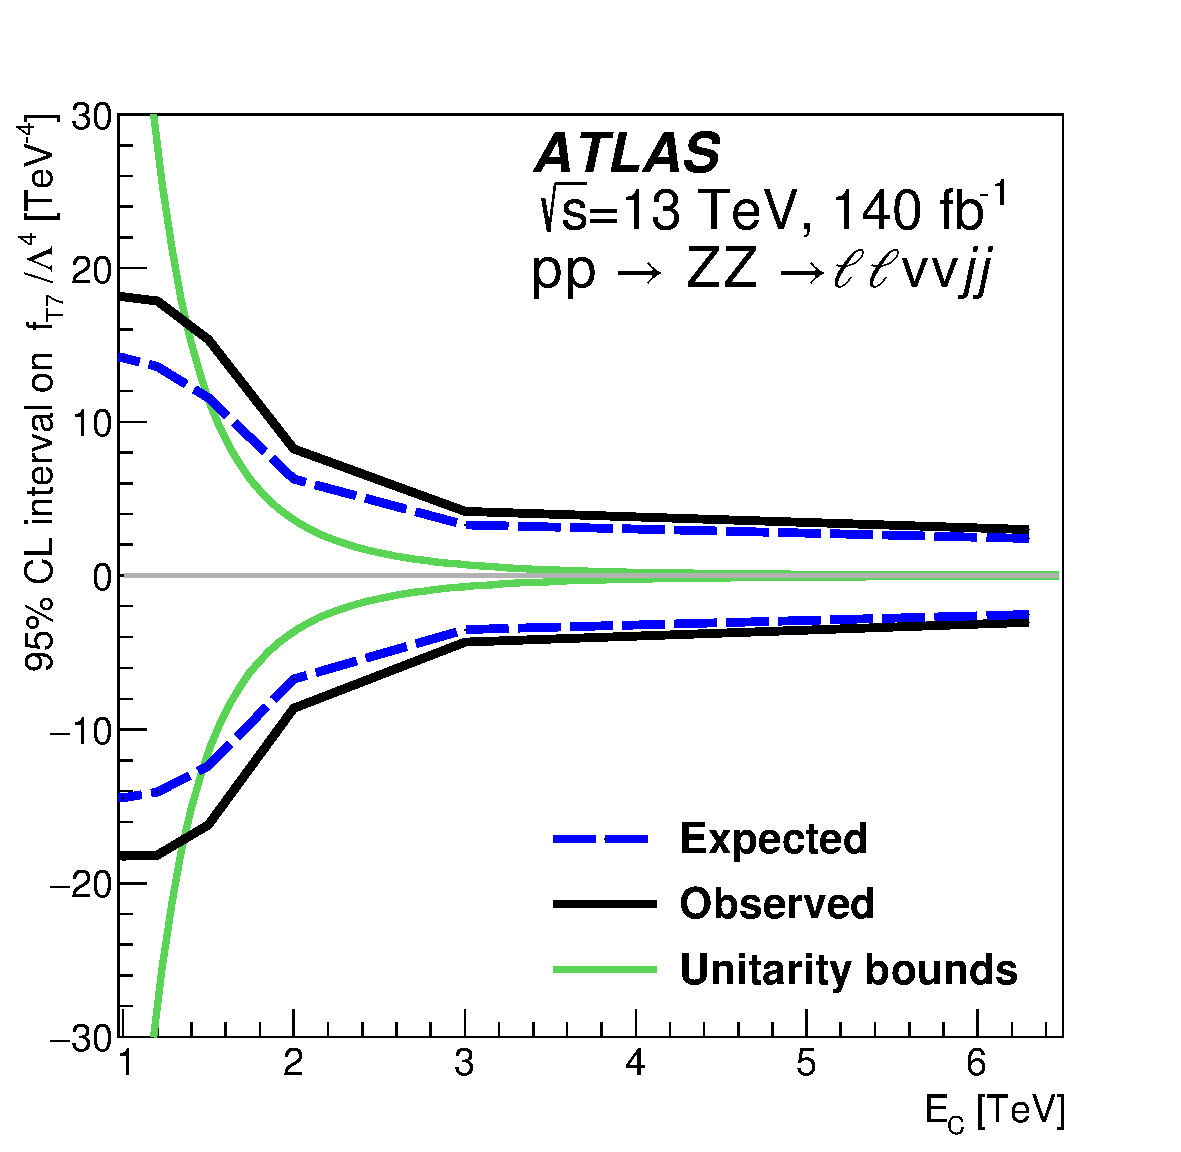
\includegraphics[width=0.32\textwidth]{figures/ch5-llvv/fig_aqgc_limit_fT7.pdf}
%         \label{fig:aqgc_fT7}
%     }
%     \hfill
%     \subfloat[]{
%         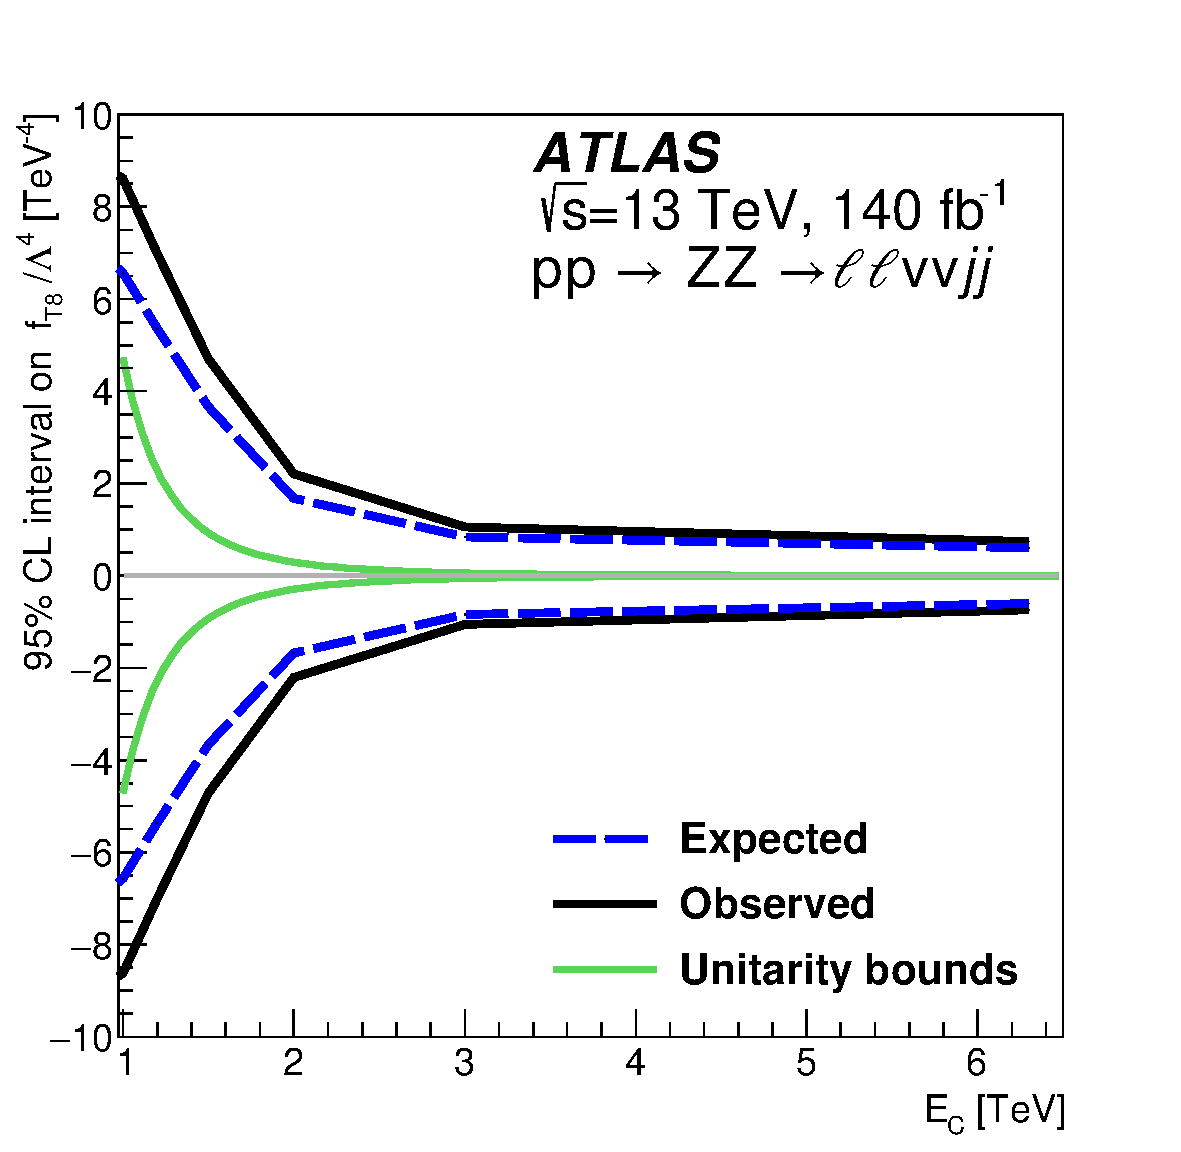
\includegraphics[width=0.32\textwidth]{figures/ch5-llvv/fig_aqgc_limit_fT8.pdf}
%         \label{fig:aqgc_fT8}
%     }
%     \hfill
%     \subfloat[]{
%         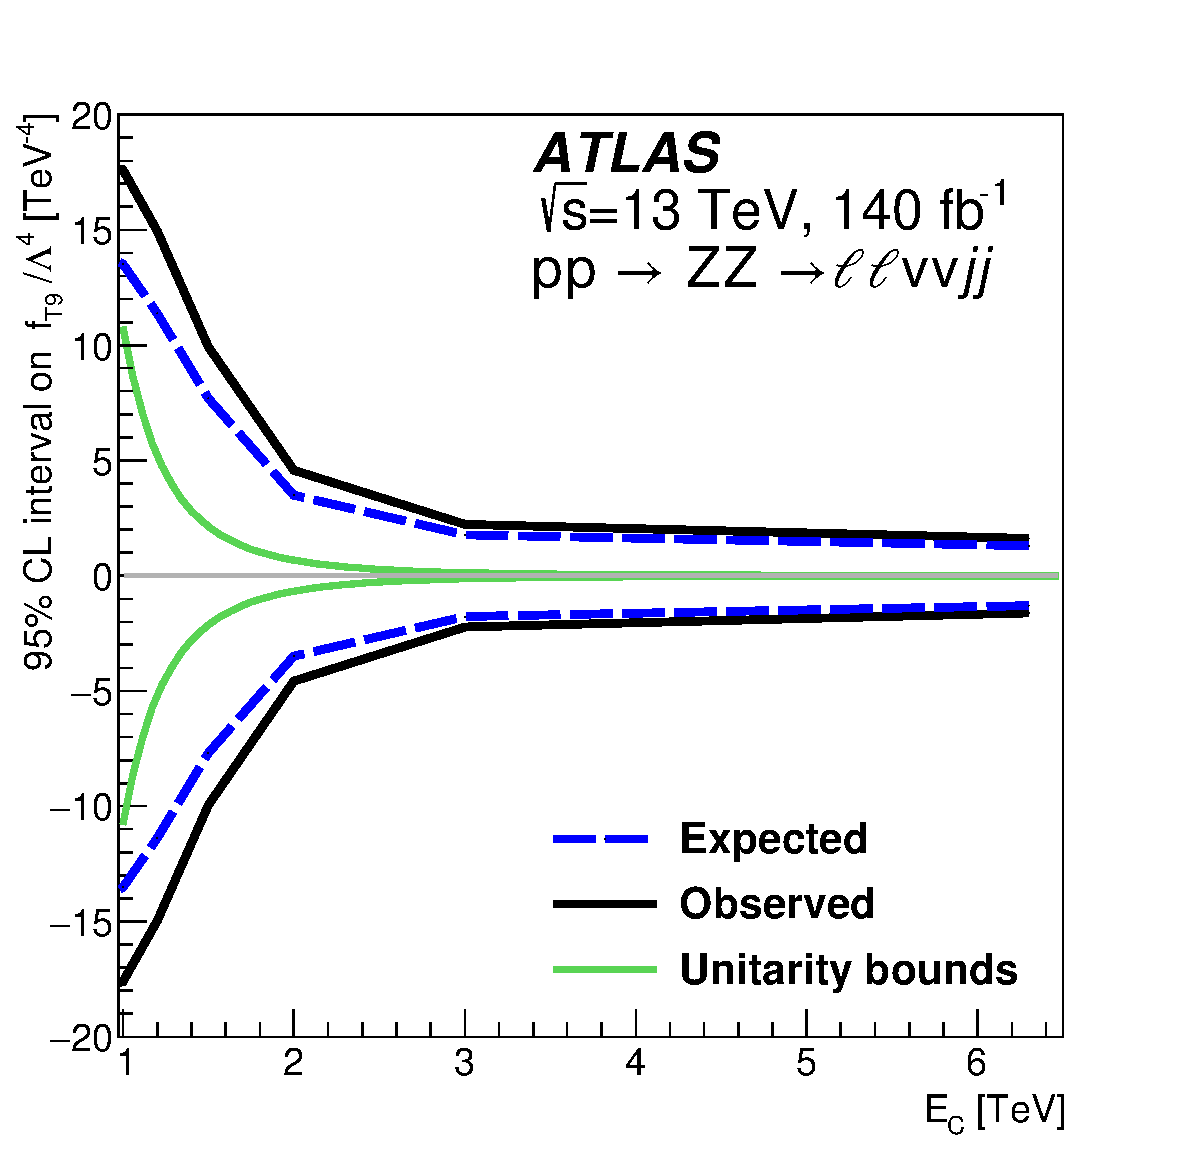
\includegraphics[width=0.32\textwidth]{figures/ch5-llvv/fig_aqgc_limit_fT9.pdf}
%         \label{fig:aqgc_fT9}
%     }
%     \caption{Expected and observed 95\% CL intervals for the Wilson coefficients $f_{\text{T}4}$ through $f_{\text{T}9}$ as a function of the EFT cut-off scale $E_{\text{c}}$. The dashed (solid) lines show the expected (observed) limits, and the solid green curve corresponds to the unitarity bounds.}
%     \label{fig:aqgc_limits_fT4_fT9}
% \end{figure}

\section{Summary of Results}

Integrated and differential cross-sections for $\text{Z}$ boson pair production in the 
$\text{ZZ} \to \ell^+\ell^- \nu\bar{\nu}$ final state are measured in both inclusive $\text{ZZ}$ and VBS-like $\text{ZZ}jj$ production modes at $\sqrt{s}=13~\text{TeV}$ using $140~\text{fb}^{-1}$ of ATLAS data. Stringent constraints are placed on neutral anomalous triple gauge couplings (aTGCs) and anomalous quartic gauge couplings (aQGCs) based on this analysis. 

The fiducial cross-sections for inclusive $\text{ZZ} \to \ell\ell\nu\nu$ and $\text{ZZ}jj \to \ell\ell\nu\nu jj$ production are measured to be $21 \pm 1~\text{fb}$ and $0.96^{+0.18}_{-0.16}~\text{fb}$, respectively, in agreement with the SM predictions of $20.1 \pm 1.1~\text{fb}$ and $0.94 \pm 0.20~\text{fb}$ from \textsc{Sherpa}+\textsc{MadGraph5} calculations. Compared with earlier measurements using a partial Run~2 dataset, the total uncertainty in the inclusive $\text{ZZ}$ fiducial cross-section is reduced from 7.0\% to 4.6\% and is now dominated by statistical uncertainty. The \textsc{Matrix} prediction for the inclusive fiducial cross-section is $21.03 \pm 0.30~\text{fb}$, reflecting improved theoretical precision from calculations including NNLO QCD and NLO electroweak corrections. The inclusive $\text{ZZ} \to \ell\ell\nu\nu$ cross-section extrapolated to the total phase space is measured to be $15.38 \pm 0.81~\text{pb}$, consistent with the SM prediction of $15.40 \pm 0.38~\text{pb}$ from \textsc{Matrix}.

Differential cross-sections for both $\text{ZZ}$ and $\text{ZZ}jj$ production are measured as functions of key kinematic observables, providing stringent tests of the SM and valuable inputs for modelling studies. The transverse momentum of the dilepton system is used to constrain anomalous neutral triple gauge couplings using both the vertex-function and SMEFT frameworks. In the vertex-function formalism, limits are set on $f_{4}^{\text{Z}}$, $f_{4}^{\gamma}$, $f_{5}^{\gamma}$, and $f_{5}^{\text{Z}}$, improving previous results in this final state by approximately a factor of 1.7. In the SMEFT interpretation, performed for the first time for this channel, limits are derived on Wilson coefficients associated with neutral aTGCs.

In the $\text{ZZ}jj$ channel, the transverse mass of the $\text{ZZ}$ system is used to constrain dimension-eight operators contributing to anomalous quartic gauge couplings. These results improve sensitivity by a factor of approximately 2--3 relative to the $4\ell jj$ channel, owing to the larger branching ratio of the $\ell\ell\nu\nu$ final state. Overall, the measurements show excellent agreement with SM predictions and significantly enhance sensitivity to physics beyond the SM in the electroweak sector.

%The fiducial and differential cross-sections for the inclusive $\text{ZZ} \to \ell\ell\nu\nu$ process have been measured with high precision using the full ATLAS Run 2 dataset. The inclusive fiducial cross-section is measured with a precision of 4.8\%, limited by statistics. All measurements show excellent agreement with SM predictions. 

%Stringent limits have been placed on anomalous triple gauge couplings, significantly constraining the phase space for new physics in the electroweak sector.
%\input{chapters/Ch5-ZZxs/5_8_dnn}

